\documentclass{cmspaper}
\usepackage{graphicx}
\usepackage{rotate}
\usepackage{relsize}
\usepackage{lineno}
\usepackage{slashed}
\usepackage{slashbox}
\usepackage{url}
\newcommand{\ptll} {\ensuremath{P_T(\ell\ell)}}
\newcommand{\ptllres} {\ensuremath{P^{\rm res}_T(\ell\ell)}}
\def\ack{\section*{Acknowledgments}}

\linenumbers

%%%
\def\mrm{\mathrm}
\def\ra{\rightarrow}

%units
\newcommand{\eV}{\ensuremath{\mathrm{e\kern -0.1em V}}}
\newcommand{\TeV}{\ensuremath{\mathrm{Te\kern -0.1em V}}}
\newcommand{\GeV}{\ensuremath{\mathrm{Ge\kern -0.1em V}}}
\newcommand{\MeV}{\ensuremath{\mathrm{Me\kern -0.1em V}}}
\newcommand{\keV}{\ensuremath{\mathrm{ke\kern -0.1em V}}}
\newcommand{\GeVc}{\ensuremath{\GeV/c}}
\newcommand{\GeVcc}{\ensuremath{\GeV/{c^2}}}
\newcommand{\MeVcc}{\ensuremath{\MeV/{c^2}}}
\newcommand{\Tesla}{\ensuremath{\mathrm{T}}}
\newcommand{\m}{\ensuremath{\mathrm{m}}}
\newcommand{\cm}{\ensuremath{\mathrm{cm}}}
\newcommand{\um}{\ensuremath{\mu \mathrm{m}}}
\newcommand{\fm}{\ensuremath{\mathrm{fm}}}
\newcommand{\mm}{\ensuremath{\mathrm{mm}}}
\newcommand{\us}{\ensuremath{\mu\mathrm{s}}}
\newcommand{\ms}{\ensuremath{\mathrm{ms}}}
\newcommand{\ns}{\ensuremath{\mathrm{ns}}}
\newcommand{\ps}{\ensuremath{\mathrm{ps}}}
\newcommand{\nb}{\ensuremath{\mathrm{nb}}}
\newcommand{\pb}{\ensuremath{\mathrm{pb}}}
\newcommand{\fb}{\ensuremath{\mathrm{fb}}}
\newcommand{\ub}{\ensuremath{\mathrm{\mu b}}}
\newcommand{\nbin}{\ensuremath{\mathrm{nb}^{-1}}}
\newcommand{\pbin}{\ensuremath{\mathrm{pb}^{-1}}}
\newcommand{\fbin}{\ensuremath{\mathrm{fb}^{-1}}}
\newcommand{\ubin}{\ensuremath{\mathrm{\mu b}^{-1}}}
\newcommand{\instlumU}{\ensuremath{\cm^{-2}\mathrm{s}^{-1}}}
%%%%%%%%%%%%%
%spec symbols
\newcommand{\at}{\symbol{64}}
\newcommand{\sye}[1]{\ensuremath{~\pm #1}}
\newcommand{\ase}[2]{\ensuremath{^{~+ #1}_{~- #2}}}
\newcommand{\asi}[2]{\ensuremath{^{~- #1}_{~+ #2}}}

%particles and decay chains
\newcommand{\jp}{\ensuremath{J/\psi}}
\newcommand{\eepm}{\ensuremath{e^+ e^-}}
\newcommand{\mmpm}{\ensuremath{\mu^+ \mu^-}}
\newcommand{\ttpm}{\ensuremath{\tau^+ \tau^-}}
\newcommand{\empm}{\ensuremath{e^\pm \mu^\mp}}
\newcommand{\dy}{\ensuremath{Z/\gamma^\star}}
\newcommand{\dyee}{\ensuremath{\dy\to\eepm}}
\newcommand{\dymm}{\ensuremath{\dy\to\mmpm}}
\newcommand{\dytt}{\ensuremath{\dy\to\ttpm}}
\newcommand{\wen}{\ensuremath{W\to e\nu_{e}}}
\newcommand{\wmn}{\ensuremath{W\to\mu\nu_{\mu}}}
\newcommand{\wtn}{\ensuremath{W\to\tau\nu_{\tau}}}

\newcommand{\roots}{\ensuremath{\sqrt{s}}}
\newcommand{\lhcE}[1]{\ensuremath{\roots ={#1}~\TeV}}

\newcommand{\EE}[1]{\ensuremath{\times 10^{#1}}}
%acronyms and such
\newcommand{\pbar}{\ensuremath{\overline{p}}}
\newcommand{\ppbar}{\ensuremath{p\overline{p}}}
\newcommand{\ttbar}{\ensuremath{t\overline{t}}}
\newcommand{\bbbar}{\ensuremath{b\overline{b}}}
\newcommand{\ccbar}{\ensuremath{c\overline{c}}}
\newcommand{\qqbar}{\ensuremath{q\overline{q}}}
\newcommand{\pp}{\ensuremath{pp}}

\newcommand{\sign}{\ensuremath{\mathrm{sign}}}
\newcommand{\rphi}{\text{$r$-$\phi$}}
\newcommand{\etaphi}{\text{$\eta$-$\phi$}}
\newcommand{\rz}{\text{$r$-$z$}}
\newcommand{\pt}{\ensuremath{p_T}}
\newcommand{\Ht}{\ensuremath{H_T}}
\newcommand{\met} {\ensuremath{E\!\!\!\!/_T}}
%%\newcommand{\tcmet}{\ensuremath{\met^\mrm{tc}}}
\newcommand{\tcmet}{\ensuremath{\mrm{tcMET}}}
\newcommand{\jets}{\ensuremath{\mrm{jets}}}
\newcommand{\isotk}{\ensuremath{I_\mrm{trk}}}
\newcommand{\isocal}{\ensuremath{I_\mrm{cal}}}
\newcommand{\mll}{\ensuremath{M_{\ell\ell}}}

\newcommand{\intLumi}{\ensuremath{4.98~\fbin}}


\begin{document}

%==============================================================================
% title page for many authors
%
\begin{titlepage}
\title{Search for New Physics in the Same Sign Dilepton final state with b Jets and Missing Energy at the LHC}

  \begin{Authlist}
    D.~ Barge, C.~Campagnari, D.~Kovalskyi, V.~Krutelyov
    \Instfoot{ucsb}{University of California, Santa Barbara}
    W.~Andrews, G.~Cerati, D.~Evans, F.~Golf, I.~MacNeill, S.~Padhi, Y.~Tu, F.~W\"urthwein, A.~Yagil, J.~Yoo
    \Instfoot{ucsd}{University of California, San Diego}
    L.~Bauerdick, K.~Burkett, I.~Fisk, Y.~Gao, O.~Gutsche, B.~Hooberman, S.~Jindariani, J.~Linacre,
    V.~Martinez~Outschoorn
    \Instfoot{fnal}{Fermi National Accelerator Laboratory, Batavia, Illinois}
  \end{Authlist}

\begin{abstract}
A search for New Physics in the same sign dilepton final state with at least two $b$-jets 
and \met~ is performed. 
This analysis uses a data sample collected with the CMS detector
of pp collisions at a centre-of-mass energy of 7 TeV, corresponding to an integrated
luminosity of \intLumi. 
% For these searches, the dominant background is from \ttbar\ events. 
No excess above the standard model background expectation is observed.
Upper limits at 95\% confidence level are set on the number of observed events.
Information on acceptance and efficiencies are provided so that our 
results can be used to confront additional models in an approximate way.
These limits are also 
used to constrain a number of new physics models.
%pMSSM as well as the simplified models 
%involving stop and sbottom productions.
\end{abstract}
\end{titlepage}

\section{Introduction}
\label{sec:intro}

After the successful operation of the Large Hadron Collider (LHC) and the CMS detector
in 2010 and 2011, and with good prospects for the future, the LHC is now ready to shed light on a number 
of open questions in Particle Physics 
such as the mechanism of electroweak (EW) symmetry breaking, or the 
new physics, Beyond the Standard Model (BSM), that stabilizes the EW scale. 

A wealth of theories that extend the Standard Model have been put forth during the past decades. Supersymmetry (SUSY) is
arguably the best motivated BSM theory --- and certainly the most 
thoroughly studied. 
Indeed, searches for SUSY are among the primary objectives of the 
CMS experiment. SUSY is exceedingly popular not 
only for its theoretical beauty but also because SUSY phenomenology 
is extremely rich, 
%in fact is can mimic almost any other new physics scenario. 
leading to a large variety of possible new signals at the LHC. 
In spite of this, the majority of SUSY studies focus on a very special 
setup: the so-called Constrained Minimal Supersymmetric Standard Model (CMSSM). 
This was justified in the preparation for discoveries as the CMSSM, 
having just a handful of new parameters, is very predicive. However, 
the simplifying assumption of universality at the GUT scale lacks a sound 
theoretical motivation. Consequently, the CMSSM should be regarded as a showcase 
model. When it comes to interpreting experimental results, it is reasonable and interesting to do this within the CMSSM because it 
provides (to some degree) an easy way to show performances, 
compare limits or reaches, etc. However, the interpretation of experimental results in the 
$(m_0,m_{1/2})$ plane risks imposing unwarranted constraints on SUSY, as many 
mass patterns and signatures that are possible a priori are not covered in the CMSSM. 
The same problem arises in any analysis that assumes a particular 
SUSY breaking scheme. 

In this document, we therefore introduce a different approach, which uses only 
minimal assumptions on the underlying SUSY parameters. In particular, given the absence of experimental guidance, we choose
not to rely on a particular SUSY breaking scheme.
Instead, we use a 19-dimensional 
parametrization of the MSSM, called the \emph{phenomenological MSSM} (pMSSM),
with parameters defined not at the GUT scale but instead at the SUSY scale 
(by convention the geometric mean of the two stop masses).
We demonstrate the feasibility of our approach by applying it to 
the 2011 CMS data-set corresponding to 1~fb$^{-1}$ of integrated luminosity.  
Using profile likelihoods, we combine 
the dijet $\alpha_T$ analysis, the opposite-sign dilepton 
analysis and the same-sign dilepton analysis and derive constraints 
on the SUSY particles with as few simplifying assumptions as possible.
Results from other SUSY analyses in CMS will be added as soon as they become available.

We first give the motivation to go beyond the CMSSM and work in 
a generic MSSM setup. After this, the pMSSM and its parametrization is defined. 
We then outline our analysis, giving details on the pMSSM points we have used, 
the detector simulation and the CMS analyses, and describe the statistical method based on 
profile likelihoods used for coping with the 19-dimensional model. Finally, we discuss our results and summarize our conclusions.


%\section{Simulated Event samples}
\label{sec:mcsignal}

In the MSSM, the scalar partners of the left- and right-handed squarks, $\tilde{q_L}$
and $\tilde{q_R}$, can mix to form mass eigenstates. These mixing effects thus leads to different fermion
masses and therefore becomes important for the third generation. The large mixing can yield sbottom ($\tilde{b_1}$)
and stop ($\tilde{t_1}$) eigenstates which are significantly lighter than other squarks. This also implies  $\tilde{b_1}$
and $\tilde{t_1}$ could be produced with larger cross sections then the light flavour squarks at the LHC. Consequently, 
the subsequent decays of $\tilde{b_1}$ and $\tilde{t_1}$ can lead to same sign dileptons in association with b quarks.
Furthermore, the $\tilde{g}\tilde{g}$ productions via $\tilde{\chi}^\pm_1$ such as $\tilde{g} \rightarrow \tilde{\chi}^{+}_{1} b \bar{t}$
can also give rise to same sign dileptons with b jets.

%\section{Search for same-sign dileptons with $b$ jets}
\label{sec:searchbtag}

This analysis is based on the same-sign dilepton search documented in AN-2011/258~\cite{ssnote2011} and corresponds to an
integrated luminosity of \intLumi. In that study we searched for events with two isolated same-sign leptons
in association with 2 additional jets and \met. Here we re-use most of the baseline event selection~\footnote{The additional 
$Z$ veto is not applied in this study} as summarized in Section~\ref{sec:eventsel} below. 
In addition, we require at least 2 b-tagged jets using Track Counting High Efficiency 
Medium (TCHEM) working point tagger~\cite{BTVPAS2011}. We refer to TCHEM with the requirement that three of the tracks have $IP$ 
significance $ > 3.3$. For this tagger the expected b-tagging efficiency is 62\% with a roughly 20\% systematic uncertainty.
The acceptance of light flavor jets is $\sim 2$\%~\cite{BTVPAS2011}.

\subsection{Event Selection}
\label{sec:eventsel}

As mentioned previously, this search is a refinement of~\cite{ssnote2011}, and we thus discuss here only differences and briefly summarize the basic kinematics and triggers.
For more details, we refer to~\cite{ssnote2011}.

\begin{itemize}
\item At least two isolated same-sign leptons ($ee$, $e\mu$, and $\mu\mu$) with $|\eta| < 2.4$.
\item We require both leptons to have $p_T>$20 GeV.
\item We tighten the isolation cut on the leptons to 0.1.
\item At least two particle flow jets tagged using SSVHEM tagger with $p_T > 40$ GeV and $|\eta| < 2.4$
%{\it why not 3.0 ??} 
corrected with L1FastL2L3 corrections.
\item The selected jets must be separated from the leptons by $\Delta R > 0.4$.
\item \met $> 30$ GeV.
\item We remove dilepton events with invariant mass $M_{ll} < 8$ GeV.
%{\it switched to tighter mll cut because we can.}
\end{itemize}

More details are found in Reference~\cite{ssnote2011}.

\subsection{Event Yields and Background Estimation}
\label{eventsel}

The results of this search in the above-mentioned kinematical region are summerized in Table~\ref{tab:ssyields1}.
As mentioned in the introduction, and quantified by this table, SM background is expected to be dominated by $t\bar{t}$ production
with one real and one fake lepton.
We estimate this background from the data itself using the ``Tight-To-Loose ratio'' (Fake Rate) method~\cite{frmethod}.
Electron charge mis-reconstruction is estimated by weighting opposite-sign dilepton events that pass all our cuts
by a charge flip rate obtained form single electron Monte Carlo as described in detail in~\cite{ssnote2011}.
The probability for muons to be reconstructed with the wrong sign in the relevant momemtum range is negligible.
Both of these techniques are described in more detail in~\cite{ssnote2011}.
Systematic errors on these two estimates are 50\% and 25\% respectively.

In addition, we use MC to estimate contributions from the following additional SM production processes.
All of these are quite small.

\begin{itemize}
\item $qqW^\pm W^\pm, WWW, t\bar{t}W$, and double parton $W^\pm W^\pm$ with two real leptons in the final state.
\item $WZ$ and $ZZ$ with two real leptons in the final state.
\item $W\gamma$ with one real lepton and a photon conversion. This background is a priori not estimated by the fake rate method
because the photon is generally isolated. In practice, this background is completely negligible.
\end{itemize}

{\it Need to update the tables to include the remaining MC bkg as the MC becomes available !!!}

\newcommand{\ttdilS}{\ensuremath{\ttbar\to\ell\ell X}}
\newcommand{\ttslbS}{\ensuremath{\ttbar\to\ell(b\to\ell) X}}
\newcommand{\ttsloS}{\ensuremath{\ttbar\to\ell(b\!\!\!/\to\ell) X}}
\newcommand{\SFnn}{\ensuremath{N^{\rm Wj,raw}_{nn}}}

\begin{table}[h]
\begin{center}
\begin{tabular}{l | l l l l}
\hline\hline
 Source  &  ee  &  $\mu\mu$  &  e$\mu$  &  all \\
\hline
$t\overline{t}\rightarrow \ell\ell X$ &  0.469 $\pm$  0.305 &  0.000 $\pm$  0.199 &  1.133 $\pm$  0.580 &  1.603 $\pm$  0.656\\
$t\overline{t}$ other &  0.000 $\pm$  0.199 &  0.000 $\pm$  0.199 &  0.000 $\pm$  0.199 &  0.000 $\pm$  0.199\\
$t\overline{t}\rightarrow \ell(b\rightarrow \ell)X$ &  0.000 $\pm$  0.199 &  0.193 $\pm$  0.143 &  0.000 $\pm$  0.199 &  0.193 $\pm$  0.143\\
$t\overline{t}\rightarrow \ell(\slashed{b}\rightarrow \ell)X$ &  0.563 $\pm$  0.399 &  0.000 $\pm$  0.199 &  0.143 $\pm$  0.131 &  0.706 $\pm$  0.420\\
\hline
$t$, s-channel &  0.000 $\pm$  0.057 &  0.000 $\pm$  0.057 &  0.000 $\pm$  0.057 &  0.000 $\pm$  0.057\\
$t$, t-channel &  0.077 $\pm$  0.077 &  0.000 $\pm$  0.055 &  0.000 $\pm$  0.055 &  0.077 $\pm$  0.077\\
$tW$ &  0.000 $\pm$  0.045 &  0.000 $\pm$  0.045 &  0.016 $\pm$  0.045 &  0.016 $\pm$  0.045\\
\hline
$Z\rightarrow ee$ &  0.000 $\pm$  0.429 &  0.000 $\pm$  0.429 &  0.000 $\pm$  0.429 &  0.000 $\pm$  0.429\\
$Z\rightarrow\mu\mu$ &  0.000 $\pm$  0.429 &  0.000 $\pm$  0.429 &  0.000 $\pm$  0.429 &  0.000 $\pm$  0.429\\
$Z\rightarrow\tau\tau$ &  0.000 $\pm$  0.429 &  0.000 $\pm$  0.429 &  0.000 $\pm$  0.429 &  0.000 $\pm$  0.429\\
$W$+jets &  0.000 $\pm$  1.808 &  0.000 $\pm$  1.808 &  0.000 $\pm$  1.808 &  0.000 $\pm$  1.808\\
$WW$ &  0.000 $\pm$  0.019 &  0.000 $\pm$  0.019 &  0.000 $\pm$  0.019 &  0.000 $\pm$  0.019\\
\hline
V$\gamma$ &  0.000 $\pm$  0.248 &  0.000 $\pm$  0.248 &  0.000 $\pm$  0.248 &  0.000 $\pm$  0.248\\
$W\gamma^{*}\rightarrow\ell\nu e e$ &  0.000 $\pm$  0.097 &  0.000 $\pm$  0.097 &  0.000 $\pm$  0.097 &  0.000 $\pm$  0.097\\
$W\gamma^{*}\rightarrow\ell\nu\mu\mu$ &  0.000 $\pm$  0.075 &  0.000 $\pm$  0.075 &  0.000 $\pm$  0.075 &  0.000 $\pm$  0.075\\
$W\gamma^{*}\rightarrow\ell\nu\tau\tau$ &  0.000 $\pm$  0.028 &  0.000 $\pm$  0.028 &  0.000 $\pm$  0.028 &  0.000 $\pm$  0.028\\
$WZ$ &  0.034 $\pm$  0.012 &  0.017 $\pm$  0.008 &  0.031 $\pm$  0.012 &  0.082 $\pm$  0.019\\
$ZZ$ &   0.000 $\pm$   0.000 &  0.001 $\pm$  0.001 &  0.002 $\pm$  0.001 &  0.003 $\pm$  0.001\\
\hline
dp$W^{\pm}W^{\pm}$ &  0.000 $\pm$  0.004 &  0.000 $\pm$  0.004 &  0.000 $\pm$  0.004 &  0.000 $\pm$  0.004\\
sp$W^{-}W^{-}$ &  0.000 $\pm$  0.001 &  0.000 $\pm$  0.001 &  0.003 $\pm$  0.002 &  0.003 $\pm$  0.002\\
sp$W^{+}W^{+}$ &  0.000 $\pm$  0.006 &  0.000 $\pm$  0.006 &  0.000 $\pm$  0.006 &  0.000 $\pm$  0.006\\
$t\overline{t}\gamma$ &  0.000 $\pm$  0.059 &  0.000 $\pm$  0.059 &  0.000 $\pm$  0.059 &  0.000 $\pm$  0.059\\
$t\overline{t}W$ &  0.572 $\pm$  0.025 &  0.733 $\pm$  0.028 &  1.286 $\pm$  0.038 &  2.591 $\pm$  0.053\\
$t\overline{t}Z$ &  0.118 $\pm$  0.009 &  0.158 $\pm$  0.010 &  0.268 $\pm$  0.013 &  0.544 $\pm$  0.019\\
$WW\gamma$ &  0.000 $\pm$  0.015 &  0.000 $\pm$  0.015 &  0.000 $\pm$  0.015 &  0.000 $\pm$  0.015\\
$WWW$ &  0.001 $\pm$   0.000 &  0.001 $\pm$   0.000 &  0.001 $\pm$  0.001 &  0.003 $\pm$  0.001\\
$WWZ$ &   0.000 $\pm$   0.000 &   0.000 $\pm$   0.000 &  0.001 $\pm$  0.001 &  0.001 $\pm$  0.001\\
$WZZ$ &   0.000 $\pm$   0.000 &  0.001 $\pm$   0.000 &  0.001 $\pm$   0.000 &  0.002 $\pm$  0.001\\
$ZZZ$ &   0.000 $\pm$   0.000 &   0.000 $\pm$   0.000 &   0.000 $\pm$   0.000 &   0.000 $\pm$   0.000\\
\hline
Total MC &  1.834 $\pm$  0.509 &  1.103 $\pm$  0.146 &  2.885 $\pm$  0.597 &  5.822 $\pm$  0.797\\
\hline\hline
\hline
LM6 &  0.000 $\pm$  0.000 &  0.186 $\pm$  0.186 &  0.383 $\pm$  0.275 &  0.569 $\pm$  0.332\\
\hline\hline
\hline\hline
 SF  & 1.13 $\pm$ 0.67 & 0.30 $\pm$ 0.20 & 1.92 $\pm$ 0.74 & 3.36 $\pm$ 1.02\\
 DF  & 0.04 $\pm$ 0.12 & 0.02 $\pm$ 0.02 & 0.02 $\pm$ 0.09 & 0.08 $\pm$ 0.16\\
\hline
 SF + DF  & 1.17 $\pm$ 0.63 $\pm$ 0.58 & 0.32 $\pm$ 0.20 $\pm$ 0.16 & 1.95 $\pm$ 0.72 $\pm$ 0.97 & 3.43 $\pm$ 0.98 $\pm$ 1.72\\
\hline\hline
Charge Flips & 0.390 $\pm$ 0.032 $\pm$ 0.078 & - $\pm$ - & 0.544 $\pm$ 0.032 $\pm$ 0.109 & 0.934 $\pm$ 0.045 $\pm$ 0.187\\
\hline\hline
\hline
MC Pred &  0.725 $\pm$  0.029 $\pm$  0.362 &  0.912 $\pm$  0.031 $\pm$  0.456 &  1.595 $\pm$  0.042 $\pm$  0.797 &  3.231 $\pm$  0.059 $\pm$  1.616\\
\hline\hline
Total Pred &  2.281 $\pm$  0.633 $\pm$  0.691 &  1.232 $\pm$  0.199 $\pm$  0.483 &  4.086 $\pm$  0.725 $\pm$  1.263 &  7.600 $\pm$  0.983 $\pm$  2.365\\
\hline\hline
data & 2 & 2 & 3 & 7\\
\hline\hline
\end{tabular}

\end{center}
\caption{\label{tab:yieldBase_hpt}Observed event yields in baseline 
(\met $>$ 30 GeV, and at least 2 jets with pT $>$ 40 GeV) high-\pt\ (pT $>$ 20/10) dileptons
compared to expectations from simulation alone, and from the data-driven methods.
The {\em simulated backgrounds} contribution includes contributions from genuine  same-sign lepton
pairs (WZ, ZZ, leptons from same-sign W from single-parton, double-parton, and $t\bar{t}W$ production, etc.), 
as well as electrons from converted photons in $V\gamma$ production.
Entries with zero contributing events are reported with an uncertainty corresponding to one event.
This uncertainty is not added to the total MC contribution.
Systematic uncertainties (the second uncertainty if present)
 are displayed only for the final combined type of background, no systematic
uncertainty is added for estimates with zero entries.
Systematic uncertainties are 100\% correlated among the channels.
}
\end{table}

\clearpage

\begin{table}[hbt]
\begin{center}
\begin{tabular}{l | l l l l}
\hline\hline
 Source  &  ee  &  $\mu\mu$  &  e$\mu$  &  all \\
\hline
$t\overline{t}\rightarrow \ell\ell X$ &  0.069 $\pm$  0.199 &  0.000 $\pm$  0.199 &  0.000 $\pm$  0.199 &  0.069 $\pm$  0.199\\
$t\overline{t}$ other &  0.000 $\pm$  0.199 &  0.000 $\pm$  0.199 &  0.000 $\pm$  0.199 &  0.000 $\pm$  0.199\\
$t\overline{t}\rightarrow \ell(b\rightarrow \ell)X$ &  0.000 $\pm$  0.199 &  0.000 $\pm$  0.199 &  0.000 $\pm$  0.199 &  0.000 $\pm$  0.199\\
$t\overline{t}\rightarrow \ell(\slashed{b}\rightarrow \ell)X$ &  0.266 $\pm$  0.266 &  0.000 $\pm$  0.199 &  0.128 $\pm$  0.128 &  0.394 $\pm$  0.295\\
\hline
$t$, s-channel &  0.000 $\pm$  0.057 &  0.000 $\pm$  0.057 &  0.000 $\pm$  0.057 &  0.000 $\pm$  0.057\\
$t$, t-channel &  0.000 $\pm$  0.055 &  0.000 $\pm$  0.055 &  0.000 $\pm$  0.055 &  0.000 $\pm$  0.055\\
$tW$ &  0.000 $\pm$  0.045 &  0.000 $\pm$  0.045 &  0.000 $\pm$  0.045 &  0.000 $\pm$  0.045\\
\hline
$Z\rightarrow ee$ &  0.000 $\pm$  0.429 &  0.000 $\pm$  0.429 &  0.000 $\pm$  0.429 &  0.000 $\pm$  0.429\\
$Z\rightarrow\mu\mu$ &  0.000 $\pm$  0.429 &  0.000 $\pm$  0.429 &  0.000 $\pm$  0.429 &  0.000 $\pm$  0.429\\
$Z\rightarrow\tau\tau$ &  0.000 $\pm$  0.429 &  0.000 $\pm$  0.429 &  0.000 $\pm$  0.429 &  0.000 $\pm$  0.429\\
$W$+jets &  0.000 $\pm$  1.808 &  0.000 $\pm$  1.808 &  0.000 $\pm$  1.808 &  0.000 $\pm$  1.808\\
$WW$ &  0.000 $\pm$  0.019 &  0.000 $\pm$  0.019 &  0.000 $\pm$  0.019 &  0.000 $\pm$  0.019\\
\hline
V$\gamma$ &  0.000 $\pm$  0.248 &  0.000 $\pm$  0.248 &  0.000 $\pm$  0.248 &  0.000 $\pm$  0.248\\
$W\gamma^{*}\rightarrow\ell\nu e e$ &  0.000 $\pm$  0.097 &  0.000 $\pm$  0.097 &  0.000 $\pm$  0.097 &  0.000 $\pm$  0.097\\
$W\gamma^{*}\rightarrow\ell\nu\mu\mu$ &  0.000 $\pm$  0.075 &  0.000 $\pm$  0.075 &  0.000 $\pm$  0.075 &  0.000 $\pm$  0.075\\
$W\gamma^{*}\rightarrow\ell\nu\tau\tau$ &  0.000 $\pm$  0.028 &  0.000 $\pm$  0.028 &  0.000 $\pm$  0.028 &  0.000 $\pm$  0.028\\
$WZ$ &  0.009 $\pm$  0.006 &  0.001 $\pm$  0.003 &  0.006 $\pm$  0.004 &  0.016 $\pm$  0.008\\
$ZZ$ &  0.000 $\pm$   0.000 &  0.000 $\pm$   0.000 &   0.000 $\pm$   0.000 &   0.000 $\pm$   0.000\\
\hline
dp$W^{\pm}W^{\pm}$ &  0.000 $\pm$  0.004 &  0.000 $\pm$  0.004 &  0.000 $\pm$  0.004 &  0.000 $\pm$  0.004\\
sp$W^{-}W^{-}$ &  0.000 $\pm$  0.001 &  0.000 $\pm$  0.001 &  0.001 $\pm$  0.001 &  0.001 $\pm$  0.001\\
sp$W^{+}W^{+}$ &  0.000 $\pm$  0.006 &  0.000 $\pm$  0.006 &  0.000 $\pm$  0.006 &  0.000 $\pm$  0.006\\
$t\overline{t}\gamma$ &  0.000 $\pm$  0.059 &  0.000 $\pm$  0.059 &  0.000 $\pm$  0.059 &  0.000 $\pm$  0.059\\
$t\overline{t}W$ &  0.315 $\pm$  0.020 &  0.363 $\pm$  0.021 &  0.643 $\pm$  0.028 &  1.321 $\pm$  0.040\\
$t\overline{t}Z$ &  0.061 $\pm$  0.007 &  0.086 $\pm$  0.008 &  0.167 $\pm$  0.012 &  0.314 $\pm$  0.016\\
$WW\gamma$ &  0.000 $\pm$  0.015 &  0.000 $\pm$  0.015 &  0.000 $\pm$  0.015 &  0.000 $\pm$  0.015\\
$WWW$ &   0.000 $\pm$   0.000 &   0.000 $\pm$   0.000 &  0.001 $\pm$  0.001 &  0.002 $\pm$  0.001\\
$WWZ$ &  0.000 $\pm$   0.000 &  0.000 $\pm$   0.000 &  0.000 $\pm$   0.000 &  0.000 $\pm$   0.000\\
$WZZ$ &   0.000 $\pm$   0.000 &  0.000 $\pm$   0.000 &   0.000 $\pm$   0.000 &   0.000 $\pm$   0.000\\
$ZZZ$ &  0.000 $\pm$   0.000 &   0.000 $\pm$   0.000 &   0.000 $\pm$   0.000 &   0.000 $\pm$   0.000\\
\hline
Total MC &  0.721 $\pm$  0.276 &  0.451 $\pm$  0.022 &  0.946 $\pm$  0.131 &  2.118 $\pm$  0.306\\
\hline\hline
\hline
LM6 &  0.000 $\pm$  0.000 &  0.000 $\pm$  0.000 &  0.000 $\pm$  0.000 &  0.000 $\pm$  0.000\\
\hline\hline
\hline\hline
 SF  & 0.27 $\pm$ 0.54 & 0.00 $\pm$ 0.37 & 0.54 $\pm$ 0.59 & 0.81 $\pm$ 0.74\\
 DF  & 0.00 $\pm$ 0.14 & 0.00 $\pm$ 0.10 & 0.00 $\pm$ 0.16 & 0.00 $\pm$ 0.16\\
\hline
 SF + DF  & 0.27 $\pm$ 0.45 $\pm$ 0.14 & 0.00 $\pm$ 0.31 $\pm$ 0.00 & 0.54 $\pm$ 0.50 $\pm$ 0.27 & 0.81 $\pm$ 0.67 $\pm$ 0.40\\
\hline\hline
Charge Flips & 0.036 $\pm$ 0.010 $\pm$ 0.007 & - $\pm$ - & 0.069 $\pm$ 0.012 $\pm$ 0.014 & 0.104 $\pm$ 0.015 $\pm$ 0.021\\
\hline\hline
\hline
MC Pred &  0.386 $\pm$  0.022 $\pm$  0.193 &  0.451 $\pm$  0.022 $\pm$  0.225 &  0.818 $\pm$  0.031 $\pm$  0.409 &  1.655 $\pm$  0.044 $\pm$  0.827\\
\hline\hline
Total Pred &  0.695 $\pm$  0.453 $\pm$  0.236 &  0.451 $\pm$  0.315 $\pm$  0.225 &  1.422 $\pm$  0.496 $\pm$  0.489 &  2.568 $\pm$  0.672 $\pm$  0.921\\
\hline\hline
data & 1 & 1 & 0 & 2\\
\hline\hline
\end{tabular}

\end{center}
\caption{\label{tab:yieldlom0_hpt}Observed event yields in high-\pt\ (pT $>$ 20/10) dileptons
passing the {\em low-$m_0$} signal selections ($H_T > $ 320 GeV, \met $>$ 50 GeV)
compared to expectations from simulation alone, and from the data-driven methods.
The {\em simulated backgrounds} contribution includes contributions from genuine  same-sign lepton
pairs (WZ, ZZ, leptons from same-sign W from single-, double-parton, and $t\bar{t}W$ production, etc.), 
as well as electrons from converted photons in $V\gamma$ production.
Entries with zero contributing events are reported with an uncertainty corresponding to one event.
This uncertainty is not added to the total MC contribution.
Systematic uncertainties (the second uncertainty if present)
 are displayed only for the final combined type of background, no systematic
uncertainty is added for estimates with zero entries.
Systematic uncertainties are 100\% correlated among the channels.
}
\end{table}
\clearpage

\begin{table}[hbt]
\begin{center}
\begin{tabular}{l | l l l l}
\hline\hline
 Source  &  ee  &  $\mu\mu$  &  e$\mu$  &  all \\
\hline
$t\overline{t}\rightarrow \ell\ell X$ &  0.000 $\pm$  0.199 &  0.000 $\pm$  0.199 &  0.000 $\pm$  0.199 &  0.000 $\pm$  0.199\\
$t\overline{t}$ other &  0.000 $\pm$  0.199 &  0.000 $\pm$  0.199 &  0.000 $\pm$  0.199 &  0.000 $\pm$  0.199\\
$t\overline{t}\rightarrow \ell(b\rightarrow \ell)X$ &  0.000 $\pm$  0.199 &  0.000 $\pm$  0.199 &  0.000 $\pm$  0.199 &  0.000 $\pm$  0.199\\
$t\overline{t}\rightarrow \ell(\slashed{b}\rightarrow \ell)X$ &  0.266 $\pm$  0.266 &  0.000 $\pm$  0.199 &  0.000 $\pm$  0.199 &  0.266 $\pm$  0.266\\
\hline
$t$, s-channel &  0.000 $\pm$  0.057 &  0.000 $\pm$  0.057 &  0.000 $\pm$  0.057 &  0.000 $\pm$  0.057\\
$t$, t-channel &  0.000 $\pm$  0.055 &  0.000 $\pm$  0.055 &  0.000 $\pm$  0.055 &  0.000 $\pm$  0.055\\
$tW$ &  0.000 $\pm$  0.045 &  0.000 $\pm$  0.045 &  0.000 $\pm$  0.045 &  0.000 $\pm$  0.045\\
\hline
$Z\rightarrow ee$ &  0.000 $\pm$  0.429 &  0.000 $\pm$  0.429 &  0.000 $\pm$  0.429 &  0.000 $\pm$  0.429\\
$Z\rightarrow\mu\mu$ &  0.000 $\pm$  0.429 &  0.000 $\pm$  0.429 &  0.000 $\pm$  0.429 &  0.000 $\pm$  0.429\\
$Z\rightarrow\tau\tau$ &  0.000 $\pm$  0.429 &  0.000 $\pm$  0.429 &  0.000 $\pm$  0.429 &  0.000 $\pm$  0.429\\
$W$+jets &  0.000 $\pm$  1.808 &  0.000 $\pm$  1.808 &  0.000 $\pm$  1.808 &  0.000 $\pm$  1.808\\
$WW$ &  0.000 $\pm$  0.019 &  0.000 $\pm$  0.019 &  0.000 $\pm$  0.019 &  0.000 $\pm$  0.019\\
\hline
V$\gamma$ &  0.000 $\pm$  0.248 &  0.000 $\pm$  0.248 &  0.000 $\pm$  0.248 &  0.000 $\pm$  0.248\\
$W\gamma^{*}\rightarrow\ell\nu e e$ &  0.000 $\pm$  0.097 &  0.000 $\pm$  0.097 &  0.000 $\pm$  0.097 &  0.000 $\pm$  0.097\\
$W\gamma^{*}\rightarrow\ell\nu\mu\mu$ &  0.000 $\pm$  0.075 &  0.000 $\pm$  0.075 &  0.000 $\pm$  0.075 &  0.000 $\pm$  0.075\\
$W\gamma^{*}\rightarrow\ell\nu\tau\tau$ &  0.000 $\pm$  0.028 &  0.000 $\pm$  0.028 &  0.000 $\pm$  0.028 &  0.000 $\pm$  0.028\\
$WZ$ &  0.000 $\pm$  0.003 &  0.001 $\pm$  0.003 &  0.004 $\pm$  0.004 &  0.005 $\pm$  0.004\\
$ZZ$ &  0.000 $\pm$   0.000 &  0.000 $\pm$   0.000 &  0.000 $\pm$   0.000 &  0.000 $\pm$   0.000\\
\hline
dp$W^{\pm}W^{\pm}$ &  0.000 $\pm$  0.004 &  0.000 $\pm$  0.004 &  0.000 $\pm$  0.004 &  0.000 $\pm$  0.004\\
sp$W^{-}W^{-}$ &  0.000 $\pm$  0.001 &  0.000 $\pm$  0.001 &  0.001 $\pm$  0.001 &  0.001 $\pm$  0.001\\
sp$W^{+}W^{+}$ &  0.000 $\pm$  0.006 &  0.000 $\pm$  0.006 &  0.000 $\pm$  0.006 &  0.000 $\pm$  0.006\\
$t\overline{t}\gamma$ &  0.000 $\pm$  0.059 &  0.000 $\pm$  0.059 &  0.000 $\pm$  0.059 &  0.000 $\pm$  0.059\\
$t\overline{t}W$ &  0.143 $\pm$  0.013 &  0.168 $\pm$  0.014 &  0.302 $\pm$  0.019 &  0.614 $\pm$  0.027\\
$t\overline{t}Z$ &  0.031 $\pm$  0.005 &  0.046 $\pm$  0.006 &  0.091 $\pm$  0.008 &  0.168 $\pm$  0.011\\
$WW\gamma$ &  0.000 $\pm$  0.015 &  0.000 $\pm$  0.015 &  0.000 $\pm$  0.015 &  0.000 $\pm$  0.015\\
$WWW$ &   0.000 $\pm$   0.000 &   0.000 $\pm$   0.000 &  0.001 $\pm$   0.000 &  0.001 $\pm$  0.001\\
$WWZ$ &  0.000 $\pm$   0.000 &  0.000 $\pm$   0.000 &  0.000 $\pm$   0.000 &  0.000 $\pm$   0.000\\
$WZZ$ &  0.000 $\pm$   0.000 &  0.000 $\pm$   0.000 &  0.000 $\pm$   0.000 &  0.000 $\pm$   0.000\\
$ZZZ$ &  0.000 $\pm$   0.000 &  0.000 $\pm$   0.000 &  0.000 $\pm$   0.000 &  0.000 $\pm$   0.000\\
\hline
Total MC &  0.441 $\pm$  0.267 &  0.216 $\pm$  0.015 &  0.400 $\pm$  0.021 &  1.056 $\pm$  0.268\\
\hline\hline
\hline
LM6 &  0.000 $\pm$  0.000 &  0.000 $\pm$  0.000 &  0.000 $\pm$  0.000 &  0.000 $\pm$  0.000\\
\hline\hline
\hline\hline
 SF  & 0.00 $\pm$ 0.58 & 0.00 $\pm$ 0.37 & 0.15 $\pm$ 0.54 & 0.15 $\pm$ 0.54\\
 DF  & 0.00 $\pm$ 0.14 & 0.00 $\pm$ 0.10 & 0.00 $\pm$ 0.16 & 0.00 $\pm$ 0.16\\
\hline
 SF + DF  & 0.00 $\pm$ 0.50 $\pm$ 0.00 & 0.00 $\pm$ 0.31 $\pm$ 0.00 & 0.15 $\pm$ 0.44 $\pm$ 0.07 & 0.15 $\pm$ 0.44 $\pm$ 0.07\\
\hline\hline
Charge Flips & 0.011 $\pm$ 0.004 $\pm$ 0.002 & - $\pm$ - & 0.016 $\pm$ 0.005 $\pm$ 0.003 & 0.027 $\pm$ 0.006 $\pm$ 0.005\\
\hline\hline
\hline
MC Pred &  0.175 $\pm$  0.014 $\pm$  0.087 &  0.216 $\pm$  0.015 $\pm$  0.108 &  0.400 $\pm$  0.021 $\pm$  0.200 &  0.790 $\pm$  0.030 $\pm$  0.395\\
\hline\hline
Total Pred &  0.186 $\pm$  0.501 $\pm$  0.087 &  0.216 $\pm$  0.315 $\pm$  0.108 &  0.565 $\pm$  0.438 $\pm$  0.213 &  0.966 $\pm$  0.439 $\pm$  0.402\\
\hline\hline
data & 1 & 0 & 0 & 1\\
\hline\hline
\end{tabular}

\end{center}
\caption{\label{tab:yieldhim0_hpt}Observed event yields in high-\pt\ (pT $>$ 20/10) dileptons
passing the {\em high-$m_0$} signal selections ($H_T > 440$ GeV, \met $>$ 50 GeV)
compared to expectations from simulation alone, and from the data-driven methods.
The {\em simulated backgrounds} contribution includes contributions from genuine  same-sign lepton
pairs (WZ, ZZ, leptons from same-sign W from single-, double-parton, and $t\bar{t}W$ production, etc.), 
as well as electrons from converted photons in $V\gamma$ production.
Entries with zero contributing events are reported with an uncertainty corresponding to one event.
This uncertainty is not added to the total MC contribution.
Systematic uncertainties (the second uncertainty if present)
 are displayed only for the final combined type of background, no systematic
uncertainty is added for estimates with zero entries.
Systematic uncertainties are 100\% correlated among the channels.
}
\end{table}
\clearpage

\begin{table}[hbt]
\begin{center}
\begin{tabular}{l | l l l l}
\hline\hline
 Source  &  ee  &  $\mu\mu$  &  e$\mu$  &  all \\
\hline
$t\overline{t}\rightarrow \ell\ell X$ &  0.000 $\pm$  0.199 &  0.000 $\pm$  0.199 &  0.000 $\pm$  0.199 &  0.000 $\pm$  0.199\\
$t\overline{t}$ other &  0.000 $\pm$  0.199 &  0.000 $\pm$  0.199 &  0.000 $\pm$  0.199 &  0.000 $\pm$  0.199\\
$t\overline{t}\rightarrow \ell(b\rightarrow \ell)X$ &  0.000 $\pm$  0.199 &  0.000 $\pm$  0.199 &  0.000 $\pm$  0.199 &  0.000 $\pm$  0.199\\
$t\overline{t}\rightarrow \ell(\slashed{b}\rightarrow \ell)X$ &  0.000 $\pm$  0.199 &  0.000 $\pm$  0.199 &  0.000 $\pm$  0.199 &  0.000 $\pm$  0.199\\
\hline
$t$, s-channel &  0.000 $\pm$  0.057 &  0.000 $\pm$  0.057 &  0.000 $\pm$  0.057 &  0.000 $\pm$  0.057\\
$t$, t-channel &  0.000 $\pm$  0.055 &  0.000 $\pm$  0.055 &  0.000 $\pm$  0.055 &  0.000 $\pm$  0.055\\
$tW$ &  0.000 $\pm$  0.045 &  0.000 $\pm$  0.045 &  0.000 $\pm$  0.045 &  0.000 $\pm$  0.045\\
\hline
$Z\rightarrow ee$ &  0.000 $\pm$  0.429 &  0.000 $\pm$  0.429 &  0.000 $\pm$  0.429 &  0.000 $\pm$  0.429\\
$Z\rightarrow\mu\mu$ &  0.000 $\pm$  0.429 &  0.000 $\pm$  0.429 &  0.000 $\pm$  0.429 &  0.000 $\pm$  0.429\\
$Z\rightarrow\tau\tau$ &  0.000 $\pm$  0.429 &  0.000 $\pm$  0.429 &  0.000 $\pm$  0.429 &  0.000 $\pm$  0.429\\
$W$+jets &  0.000 $\pm$  1.808 &  0.000 $\pm$  1.808 &  0.000 $\pm$  1.808 &  0.000 $\pm$  1.808\\
$WW$ &  0.000 $\pm$  0.019 &  0.000 $\pm$  0.019 &  0.000 $\pm$  0.019 &  0.000 $\pm$  0.019\\
\hline
V$\gamma$ &  0.000 $\pm$  0.248 &  0.000 $\pm$  0.248 &  0.000 $\pm$  0.248 &  0.000 $\pm$  0.248\\
$W\gamma^{*}\rightarrow\ell\nu e e$ &  0.000 $\pm$  0.097 &  0.000 $\pm$  0.097 &  0.000 $\pm$  0.097 &  0.000 $\pm$  0.097\\
$W\gamma^{*}\rightarrow\ell\nu\mu\mu$ &  0.000 $\pm$  0.075 &  0.000 $\pm$  0.075 &  0.000 $\pm$  0.075 &  0.000 $\pm$  0.075\\
$W\gamma^{*}\rightarrow\ell\nu\tau\tau$ &  0.000 $\pm$  0.028 &  0.000 $\pm$  0.028 &  0.000 $\pm$  0.028 &  0.000 $\pm$  0.028\\
$WZ$ &  0.005 $\pm$  0.005 &  0.000 $\pm$  0.003 &  0.000 $\pm$  0.003 &  0.005 $\pm$  0.005\\
$ZZ$ &  0.000 $\pm$   0.000 &  0.000 $\pm$   0.000 &   0.000 $\pm$   0.000 &   0.000 $\pm$   0.000\\
\hline
dp$W^{\pm}W^{\pm}$ &  0.000 $\pm$  0.004 &  0.000 $\pm$  0.004 &  0.000 $\pm$  0.004 &  0.000 $\pm$  0.004\\
sp$W^{-}W^{-}$ &  0.000 $\pm$  0.001 &  0.000 $\pm$  0.001 &  0.000 $\pm$  0.001 &  0.000 $\pm$  0.001\\
sp$W^{+}W^{+}$ &  0.000 $\pm$  0.006 &  0.000 $\pm$  0.006 &  0.000 $\pm$  0.006 &  0.000 $\pm$  0.006\\
$t\overline{t}\gamma$ &  0.000 $\pm$  0.059 &  0.000 $\pm$  0.059 &  0.000 $\pm$  0.059 &  0.000 $\pm$  0.059\\
$t\overline{t}W$ &  0.028 $\pm$  0.006 &  0.041 $\pm$  0.006 &  0.076 $\pm$  0.009 &  0.145 $\pm$  0.012\\
$t\overline{t}Z$ &  0.003 $\pm$  0.001 &  0.009 $\pm$  0.003 &  0.008 $\pm$  0.002 &  0.020 $\pm$  0.004\\
$WW\gamma$ &  0.000 $\pm$  0.015 &  0.000 $\pm$  0.015 &  0.000 $\pm$  0.015 &  0.000 $\pm$  0.015\\
$WWW$ &   0.000 $\pm$   0.000 &  0.000 $\pm$   0.000 &   0.000 $\pm$   0.000 &   0.000 $\pm$   0.000\\
$WWZ$ &  0.000 $\pm$   0.000 &  0.000 $\pm$   0.000 &  0.000 $\pm$   0.000 &  0.000 $\pm$   0.000\\
$WZZ$ &  0.000 $\pm$   0.000 &  0.000 $\pm$   0.000 &  0.000 $\pm$   0.000 &  0.000 $\pm$   0.000\\
$ZZZ$ &  0.000 $\pm$   0.000 &  0.000 $\pm$   0.000 &   0.000 $\pm$   0.000 &   0.000 $\pm$   0.000\\
\hline
Total MC &  0.036 $\pm$  0.008 &  0.049 $\pm$  0.007 &  0.085 $\pm$  0.009 &  0.170 $\pm$  0.014\\
\hline\hline
\hline
LM6 &  0.000 $\pm$  0.000 &  0.000 $\pm$  0.000 &  0.000 $\pm$  0.000 &  0.000 $\pm$  0.000\\
\hline\hline
\hline\hline
 SF  & 0.00 $\pm$ 0.58 & 0.00 $\pm$ 0.37 & 0.18 $\pm$ 0.55 & 0.18 $\pm$ 0.55\\
 DF  & 0.00 $\pm$ 0.14 & 0.00 $\pm$ 0.10 & 0.00 $\pm$ 0.16 & 0.00 $\pm$ 0.16\\
\hline
 SF + DF  & 0.00 $\pm$ 0.50 $\pm$ 0.00 & 0.00 $\pm$ 0.31 $\pm$ 0.00 & 0.18 $\pm$ 0.45 $\pm$ 0.09 & 0.18 $\pm$ 0.45 $\pm$ 0.09\\
\hline\hline
Charge Flips & 0.007 $\pm$ 0.003 $\pm$ 0.001 & - $\pm$ - & 0.010 $\pm$ 0.004 $\pm$ 0.002 & 0.017 $\pm$ 0.005 $\pm$ 0.003\\
\hline\hline
\hline
MC Pred &  0.036 $\pm$  0.008 $\pm$  0.018 &  0.049 $\pm$  0.007 $\pm$  0.025 &  0.085 $\pm$  0.009 $\pm$  0.042 &  0.170 $\pm$  0.014 $\pm$  0.085\\
\hline\hline
Total Pred &  0.043 $\pm$  0.501 $\pm$  0.018 &  0.049 $\pm$  0.315 $\pm$  0.025 &  0.270 $\pm$  0.447 $\pm$  0.097 &  0.363 $\pm$  0.447 $\pm$  0.122\\
\hline\hline
data & 1 & 0 & 1 & 2\\
\hline\hline
\end{tabular}

\end{center}
\caption{\label{tab:yieldsimple_hpt}Observed event yields in high-\pt\ (pT $>$ 20/10) dileptons
passing the {\em simplified model} signal selections ($H_T > 200$ GeV, \met $>$ 120 GeV)
compared to expectations from simulation alone, and from the data-driven methods.
The {\em simulated backgrounds} contribution includes contributions from genuine  same-sign lepton
pairs (WZ, ZZ, leptons from same-sign W from single-, double-parton, and $t\bar{t}W$ production, etc.), 
as well as electrons from converted photons in $V\gamma$ production.
Entries with zero contributing events are reported with an uncertainty corresponding to one event.
This uncertainty is not added to the total MC contribution.
Systematic uncertainties (the second uncertainty if present)
 are displayed only for the final combined type of background, no systematic
uncertainty is added for estimates with zero entries.
Systematic uncertainties are 100\% correlated among the channels.
}
\end{table}

\clearpage

\begin{table}[hbt]
\begin{center}
\begin{tabular}{l | l l l l}
\hline\hline
 Source  &  ee  &  $\mu\mu$  &  e$\mu$  &  all \\
\hline
$t\overline{t}\rightarrow \ell\ell X$ &  0.000 $\pm$  0.199 &  0.000 $\pm$  0.199 &  0.000 $\pm$  0.199 &  0.000 $\pm$  0.199\\
$t\overline{t}$ other &  0.000 $\pm$  0.199 &  0.000 $\pm$  0.199 &  0.000 $\pm$  0.199 &  0.000 $\pm$  0.199\\
$t\overline{t}\rightarrow \ell(b\rightarrow \ell)X$ &  0.000 $\pm$  0.199 &  0.000 $\pm$  0.199 &  0.000 $\pm$  0.199 &  0.000 $\pm$  0.199\\
$t\overline{t}\rightarrow \ell(\slashed{b}\rightarrow \ell)X$ &  0.000 $\pm$  0.199 &  0.000 $\pm$  0.199 &  0.000 $\pm$  0.199 &  0.000 $\pm$  0.199\\
\hline
$t$, s-channel &  0.000 $\pm$  0.057 &  0.000 $\pm$  0.057 &  0.000 $\pm$  0.057 &  0.000 $\pm$  0.057\\
$t$, t-channel &  0.000 $\pm$  0.055 &  0.000 $\pm$  0.055 &  0.000 $\pm$  0.055 &  0.000 $\pm$  0.055\\
$tW$ &  0.000 $\pm$  0.045 &  0.000 $\pm$  0.045 &  0.000 $\pm$  0.045 &  0.000 $\pm$  0.045\\
\hline
$Z\rightarrow ee$ &  0.000 $\pm$  0.429 &  0.000 $\pm$  0.429 &  0.000 $\pm$  0.429 &  0.000 $\pm$  0.429\\
$Z\rightarrow\mu\mu$ &  0.000 $\pm$  0.429 &  0.000 $\pm$  0.429 &  0.000 $\pm$  0.429 &  0.000 $\pm$  0.429\\
$Z\rightarrow\tau\tau$ &  0.000 $\pm$  0.429 &  0.000 $\pm$  0.429 &  0.000 $\pm$  0.429 &  0.000 $\pm$  0.429\\
$W$+jets &  0.000 $\pm$  1.808 &  0.000 $\pm$  1.808 &  0.000 $\pm$  1.808 &  0.000 $\pm$  1.808\\
$WW$ &  0.000 $\pm$  0.019 &  0.000 $\pm$  0.019 &  0.000 $\pm$  0.019 &  0.000 $\pm$  0.019\\
\hline
V$\gamma$ &  0.000 $\pm$  0.248 &  0.000 $\pm$  0.248 &  0.000 $\pm$  0.248 &  0.000 $\pm$  0.248\\
$W\gamma^{*}\rightarrow\ell\nu e e$ &  0.000 $\pm$  0.097 &  0.000 $\pm$  0.097 &  0.000 $\pm$  0.097 &  0.000 $\pm$  0.097\\
$W\gamma^{*}\rightarrow\ell\nu\mu\mu$ &  0.000 $\pm$  0.075 &  0.000 $\pm$  0.075 &  0.000 $\pm$  0.075 &  0.000 $\pm$  0.075\\
$W\gamma^{*}\rightarrow\ell\nu\tau\tau$ &  0.000 $\pm$  0.028 &  0.000 $\pm$  0.028 &  0.000 $\pm$  0.028 &  0.000 $\pm$  0.028\\
$WZ$ &  0.004 $\pm$  0.004 &  0.001 $\pm$  0.003 &   0.000 $\pm$  0.003 &  0.006 $\pm$  0.005\\
$ZZ$ &  0.000 $\pm$   0.000 &  0.000 $\pm$   0.000 &   0.000 $\pm$   0.000 &   0.000 $\pm$   0.000\\
\hline
dp$W^{\pm}W^{\pm}$ &  0.000 $\pm$  0.004 &  0.000 $\pm$  0.004 &  0.000 $\pm$  0.004 &  0.000 $\pm$  0.004\\
sp$W^{-}W^{-}$ &  0.000 $\pm$  0.001 &  0.000 $\pm$  0.001 &  0.001 $\pm$  0.001 &  0.001 $\pm$  0.001\\
sp$W^{+}W^{+}$ &  0.000 $\pm$  0.006 &  0.000 $\pm$  0.006 &  0.000 $\pm$  0.006 &  0.000 $\pm$  0.006\\
$t\overline{t}\gamma$ &  0.000 $\pm$  0.059 &  0.000 $\pm$  0.059 &  0.000 $\pm$  0.059 &  0.000 $\pm$  0.059\\
$t\overline{t}W$ &  0.117 $\pm$  0.012 &  0.141 $\pm$  0.013 &  0.250 $\pm$  0.017 &  0.508 $\pm$  0.025\\
$t\overline{t}Z$ &  0.017 $\pm$  0.004 &  0.026 $\pm$  0.004 &  0.053 $\pm$  0.007 &  0.096 $\pm$  0.009\\
$WW\gamma$ &  0.000 $\pm$  0.015 &  0.000 $\pm$  0.015 &  0.000 $\pm$  0.015 &  0.000 $\pm$  0.015\\
$WWW$ &  0.000 $\pm$   0.000 &   0.000 $\pm$   0.000 &   0.000 $\pm$   0.000 &   0.000 $\pm$   0.000\\
$WWZ$ &  0.000 $\pm$   0.000 &  0.000 $\pm$   0.000 &  0.000 $\pm$   0.000 &  0.000 $\pm$   0.000\\
$WZZ$ &   0.000 $\pm$   0.000 &  0.000 $\pm$   0.000 &   0.000 $\pm$   0.000 &   0.000 $\pm$   0.000\\
$ZZZ$ &  0.000 $\pm$   0.000 &  0.000 $\pm$   0.000 &  0.000 $\pm$   0.000 &  0.000 $\pm$   0.000\\
\hline
Total MC &  0.138 $\pm$  0.013 &  0.168 $\pm$  0.014 &  0.305 $\pm$  0.019 &  0.611 $\pm$  0.027\\
\hline\hline
\hline
LM6 &  0.000 $\pm$  0.000 &  0.000 $\pm$  0.000 &  0.000 $\pm$  0.000 &  0.000 $\pm$  0.000\\
\hline\hline
\hline\hline
 SF  & 0.00 $\pm$ 0.58 & 0.00 $\pm$ 0.37 & 0.15 $\pm$ 0.54 & 0.15 $\pm$ 0.54\\
 DF  & 0.00 $\pm$ 0.14 & 0.00 $\pm$ 0.10 & 0.00 $\pm$ 0.16 & 0.00 $\pm$ 0.16\\
\hline
 SF + DF  & 0.00 $\pm$ 0.50 $\pm$ 0.00 & 0.00 $\pm$ 0.31 $\pm$ 0.00 & 0.15 $\pm$ 0.44 $\pm$ 0.07 & 0.15 $\pm$ 0.44 $\pm$ 0.07\\
\hline\hline
Charge Flips & 0.014 $\pm$ 0.006 $\pm$ 0.003 & - $\pm$ - & 0.011 $\pm$ 0.005 $\pm$ 0.002 & 0.025 $\pm$ 0.008 $\pm$ 0.005\\
\hline\hline
\hline
MC Pred &  0.138 $\pm$  0.013 $\pm$  0.069 &  0.168 $\pm$  0.014 $\pm$  0.084 &  0.305 $\pm$  0.019 $\pm$  0.153 &  0.612 $\pm$  0.027 $\pm$  0.306\\
\hline\hline
Total Pred &  0.152 $\pm$  0.501 $\pm$  0.069 &  0.168 $\pm$  0.315 $\pm$  0.084 &  0.466 $\pm$  0.438 $\pm$  0.170 &  0.787 $\pm$  0.439 $\pm$  0.315\\
\hline\hline
data & 0 & 0 & 0 & 0\\
\hline\hline
\end{tabular}

\end{center}
\caption{\label{tab:yieldsnu_hpt}Observed event yields in high-\pt\ (pT $>$ 20/10) dileptons
passing the {\em pMSSW/sneutrino} signal selections ($H_T > 320$ GeV, \met $>$ 120 GeV)
compared to expectations from simulation alone, and from the data-driven methods.
The {\em simulated backgrounds} contribution includes contributions from genuine  same-sign lepton
pairs (WZ, ZZ, leptons from same-sign W from single-, double-parton, and $t\bar{t}W$ production, etc.), 
as well as electrons from converted photons in $V\gamma$ production.
Entries with zero contributing events are reported with an uncertainty corresponding to one event.
This uncertainty is not added to the total MC contribution.
Systematic uncertainties (the second uncertainty if present)
 are displayed only for the final combined type of background, no systematic
uncertainty is added for estimates with zero entries.
Systematic uncertainties are 100\% correlated among the channels.
}
\end{table}

\clearpage

The estimation
is in a good agreement with the observation. We also note that the backgrounds with respect to the inclusive same-sign
dilepton search is suppressed by an order of magnitude due to the b-tag requirements.

We have visually scanned all the events in data and provide details in Section~\ref{sec:inclresults}.

%{\it We need to add this still in the results section !!!}

\subsection{Discussion of Background Expectation From MC}
\label{sec:bkgdiscussion}

Three MC studies are presented. First, we show the origin of fake leptons in MC.
Second, we 
show explicitly the degree to which the fake rate method
accurately predicts the fake lepton background in \ttbar MC, 
and third, we present evidence for our assertion that a b-quark can not simultaneously provide a b-tag and produce a fake lepton.

We use a large \ttbar sample~\footnote{The POWHEG sample TTToLNu2Q2B\_7TeV-powheg-pythia6\_Spring11-PU\_S1\_START311\_V1G1-v1 } 
normalized to 1~fb$^{-1}$ for these studies. 
The fake rates were obtained from QCD MC as described in detail in~\cite{ssnote2011}.

We classify \ttbar background events based on truth matching to their ``parent parton''
as either ``Heavy Flavor" or ``Light Flavor". Charm quarks from W decay are classified as heavy flavor.
It is thus possible to have three heavy quarks in the same event, one of which provides the isolated lepton,
the two others the b-tags.

As is shown in Table~\ref{tab:fakeOrigin1}  about 60\% (40\%) of the fake leptons are from heavy (light) flavor.

%{\it\bf Need to sort out how much of the HF contribution is in events with W to charm decays !!! I.e. where %does the remaining
%heavy flavor bkg come from?} 

\begin{table}[hbt]
\begin{center}
\begin{tabular}{|l|c|c|c|}\hline
Same Sign Leptons & Total  & Heavy Flavor & Light Flavor  \\ \hline

$ee$ & 0.31$\pm$0.07 &  0.11$\pm$0.04 & 0.21$\pm$0.05  \\
$\mu\mu$ & 0.26$\pm$0.06 & 0.22$\pm$0.05 & 0.04$\pm$0.04 \\
$e\mu$ & 0.57$\pm$0.09 & 0.37$\pm$0.07 & 0.21$\pm$0.05 \\
total & 1.15$\pm$0.13 & 0.70$\pm$0.10 & 0.45$\pm$ 0.08 \\ \hline
\end{tabular}
\caption{ Expected number of \ttbar events in 1 fb$^{-1}$ of integrated luminosity. Uncertainties are from MC statistics.\label{tab:fakeOrigin1}}
\end{center}
\end{table}

Table~\ref{tab:fakeOrigin2} shows the same breakdown for the fake rate prediction.
Here we use an MC sample where one of the W's is forced to decay leptonically while the other is not allowed to decay
leptonically.
We use this sample as it has x10 the luminosity equivalent than the standard \ttbar sample, thus providing higher statistics for 
this test. We observe an overprediction of 30\% which appears to be primarily due to overpredicting the fakes from heavy flavor.

\begin{table}[hbt]
\begin{center}
\begin{tabular}{|l|c|c|c|}\hline
Same Sign Leptons & Total &  Heavy Flavor & Light Flavor\\ \hline
$ee$ & 0.39$\pm$0.03 & 0.20$\pm$0.02 & 0.19$\pm$0.03 \\
$\mu\mu$ & 0.36$\pm$0.03 & 0.30$\pm$0.03 & 0.06$\pm$0.01 \\
$e\mu$ & 0.76$\pm$0.05 & 0.54$\pm$0.04 & 0.22$\pm$0.03 \\
total & 1.51$\pm$0.06 & 1.04$\pm$0.05 & 0.47$\pm$0.04  \\ \hline
\end{tabular}
\caption{ Predicted number of \ttbar events in 1 fb$^{-1}$ of integrated luminosity. Uncertainties are from MC statistics.\label{tab:fakeOrigin2}}
\end{center}
\end{table}

Finally, Figure~\ref{fig:ttbar_residual} shows the minimum $\Delta R$ between one of the two b-tagged jets and 
the fake lepton in the MC after 
relaxing the jet veto cone around the lepton. 
The black line indicates the jet veto cone size. Clearly, a b-quark can not simultaneously provide a b-tag and an isolated lepton.

\begin{figure}[htb]
\begin{center}
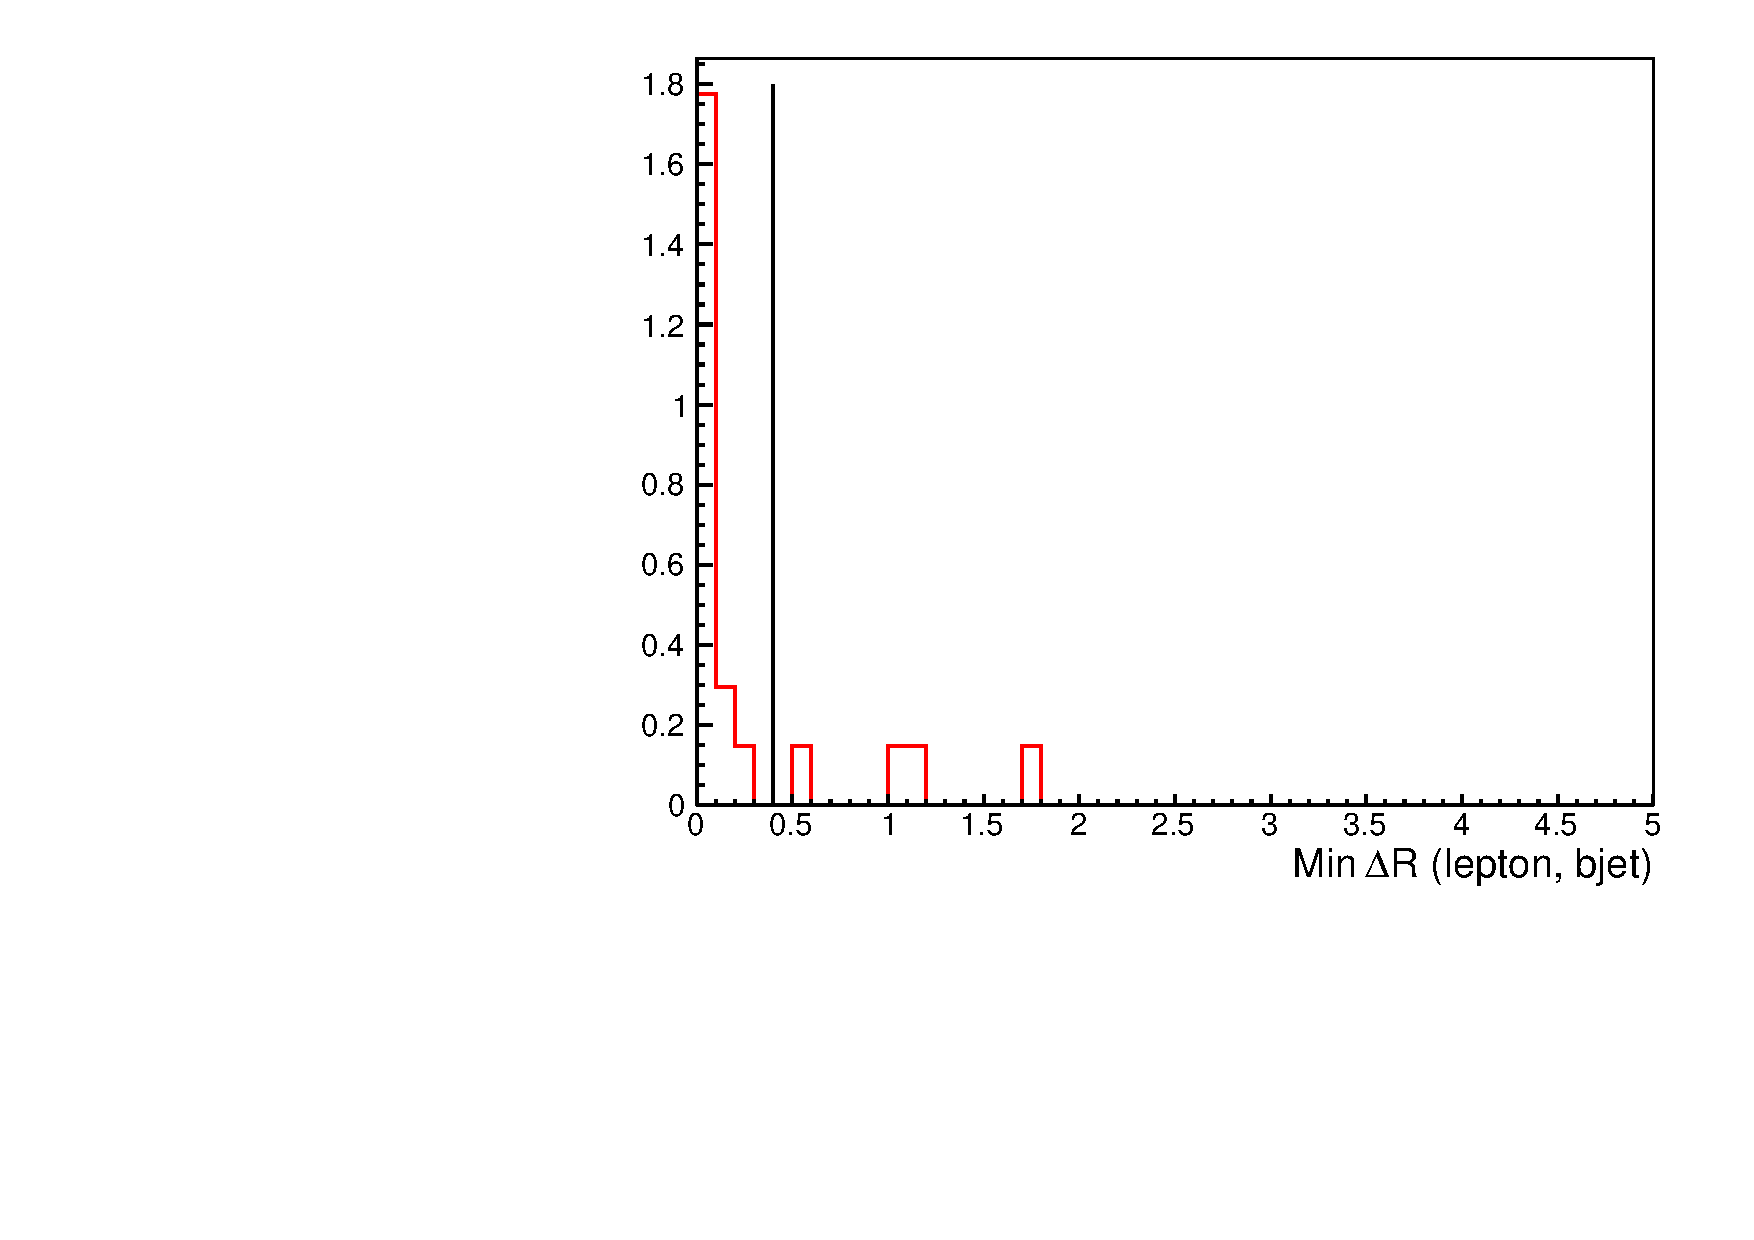
\includegraphics[width=0.6\linewidth, height=0.4\linewidth]{figs/bjetlepton.pdf}
\caption{ Minimum $\Delta R$ between the lepton and the b-tag jet in \ttbar decays.\label{fig:ttbar_residual}}
\end{center}
\end{figure}




 





\section{Baseline Event Selection}
\label{sec:eventsel}

This analysis is based on the same-sign dilepton search documented in AN-2011/468~\cite{ssnote2011} and corresponds to an
integrated luminosity of \intLumi. 
In that study we searched for events with two isolated same-sign leptons
in association with 2 additional jets and \met. 
Here we re-use most of the baseline event selection as summarized below. 
In addition, we require at least 2 b-tagged jets using Simple Secondary Vertex High Efficiency 
Medium (SSVHEM) working point tagger.
This tagger relies on reconstructed secondary vertices
with at least two tracks and an IP significance of at least 1.74 and provides a b-jet tagging 
efficiency of about 60\% with a 4\% (15\%) systematic uncertainty for jet $p_T<240 (>240)~\GeV$ 
and a tagging rate of light flavor jets in the 2--5\% range, increasing with the jet momentum~\cite{btvSyst}. 


We thus discuss here only differences and briefly summarize the basic kinematics and triggers.
For more details, we refer to~\cite{ssnote2011}.

\begin{itemize}
	\item Events have to pass one of the dilepton triggers without an HT requirement.
	\item There should be at least two isolated same-sign leptons ($ee$, $e\mu$, and $\mu\mu$) with $|\eta| < 2.5$.
	\item We require both leptons to have $p_T>$20~\GeV.
	\item We tighten the relative isolation cut on the leptons from 0.15 to 0.1.
	\item At least two particle flow jets tagged using SSVHEM tagger with $p_T > 40$ GeV and $|\eta| < 2.4$
		corrected with L1FastL2L3 corrections.
	\item The selected jets must be separated from the leptons by $\Delta R > 0.4$ (any lepton with $\pt>20~\GeV$ 
		passing the ID and isolation selections).
	\item \met $> 30$ GeV (we use pfMET).
	\item We remove dilepton events with invariant mass $M_{ll} < 8$ GeV.
	\item We veto events if a third lepton is satisfying the following 
Zveto:
	\begin{itemize}
		\item has $\pt>10~\GeV$;
		\item (an electron)  passes  $|\eta|<2.5$, and a loosened identification, 
			as the WP95 ID-only without any cut on $h/e$ in the endcaps;
		\item (for a muon) passes all identification requirements of the signal selection except 
			for the calorimeter veto requirements;
		\item has relative isolation $<0.2$; 
		\item makes an opposite-sign same-flavor pair with either of the two ``primary'' leptons such 
			that the pair has a mass within 15 GeV of the $Z$ mass.
	\end{itemize}
\end{itemize}



\section{Search Regions}
\label{sec:regions}

The count of events passing the baseline selections can 
be used to test the background predictions with the best available
stastistical precision as this is the largest sample.
We increase the sensitivity of this analysis to the models selected in 
Section~\ref{sec:intro} by considering events passing the following
search region selections applied on top of the baseline selections.

\begin{itemize}
  \item ++ region, including only positively charged lepton pairs 
    for same-sign top production via $Z^\prime$ or in MaxFV. 
    This selection reduces the fake-lepton and charge misidentification backgrounds,
    while keeping essentially all the signal, which is produced primarily from the $uu$ initial state,
    due to the available PDF luminosities.
  \item The following tighther \Ht\ and \met\ regions are defined to search for the SUSY
    production scenarios. 
    As mentioned above, all of them have four b quarks, up to two hadronically decaying W bosons,
    and at least two neutrinos and two LSPs to make up for \Ht\ and \met,
    varying between the model points.
    A region with the best expected limit is to be used in every particular case.
  \begin{enumerate}
     \item Low-\Ht\ low-\met region: $\Ht>200~\GeV, \met>50~\GeV$.
     \item Low-\Ht\ high-\met region: $\Ht>200~\GeV, \met>120~\GeV$.
     \item High-\Ht\ low-\met region: $\Ht>320~\GeV, \met>50~\GeV$.
     \item High-\Ht\ high-\met region: $\Ht>320~\GeV, \met>120~\GeV$.
  \end{enumerate}
\end{itemize}


\section{Selection Efficiency}
\label{sec:seleff}
We would like to quote our results as a cross section, or cross section limit, that is as
model independent as possible. 
For this we carefully define the acceptance, and provide enough
details about the selection efficiency within that acceptance that anybody can use their favorite Monte Carlo
generator of new physics, define an acceptance at the hard scatter level (status = 3 in Pythia), and correctly estimate
the efficiency for this new physics model to within 50\% or so (the so-called
``outreach'' program).
The same steps are done here as in the pre-tagged sample analysis~\cite{ssnote2011}
with appropriate modifications considering differences in selections of leptons
and an addition of the b-tagged jet requirements.

The event selection efficiency is a combination of 
\begin{itemize}
\item the lepton identification and isolation efficiency;
\item the efficiency of the \met\ requirement;
\item the efficiency of the \Ht\ requirement;
\item the efficiency of the b-jet tagging requirement.
\end{itemize}
We derive efficiency functions for every component using a sample of simulated events
for LM6 SUSY model point.\footnote{The LM6 cMSSM model point 
is defined by the model parameters as $m_0 = 85~\GeV$, $m_{1/2} = 400~\GeV$, $\tan\beta = 10$, $\mu>0$,
and $A_0 = 0~\GeV$.}
Applicable simulation-to-data corrections (scale factors) are also evaluated based on 
available comparisons of these effiencies in data and simulation.
As described below, the description of the lepton selections
does not require an additional scale factor,
and the correction for b-tagged jets is small with a scale factor of 0.96.

\subsection{Definition of Acceptance}
\label{sec:acceptance}
%
Lepton acceptance is defined for both leptons with $|\eta|<2.4$ and $\pt > 20~\GeV$.
The generator-level equivalent of the \Ht, $\Ht^{\rm gen}$, is comprised of the sum $\pt$ of all colored particles 
at the hard scatter level that have $\pt > 40$ GeV and $|\eta |<2.5$. 
A generator-level \met\ equivalent, $\met^{\rm~gen}$, is defined as the absolute value of the vector sum of the transverse 
momentum of all non-interacting particles, e.g. neutrinos and LSP.
%
%
\subsection{Lepton Efficiencies}
\label{sec:lepeff}
%
The electon and muon selection efficiency dependence as a function of the lepton \pt\
is shown in Fig.~\ref{fig:lepeffLM6}.
It is derived using the LM6 events passing the baseline selections applied to jets and \met.
Compared to the pre-tagged sample analysis~\cite{ssnote2011}, we obtain a slightly
lower efficiency, consistent with the tighter requirement on isolation.

\begin{figure}[h]
\begin{center}
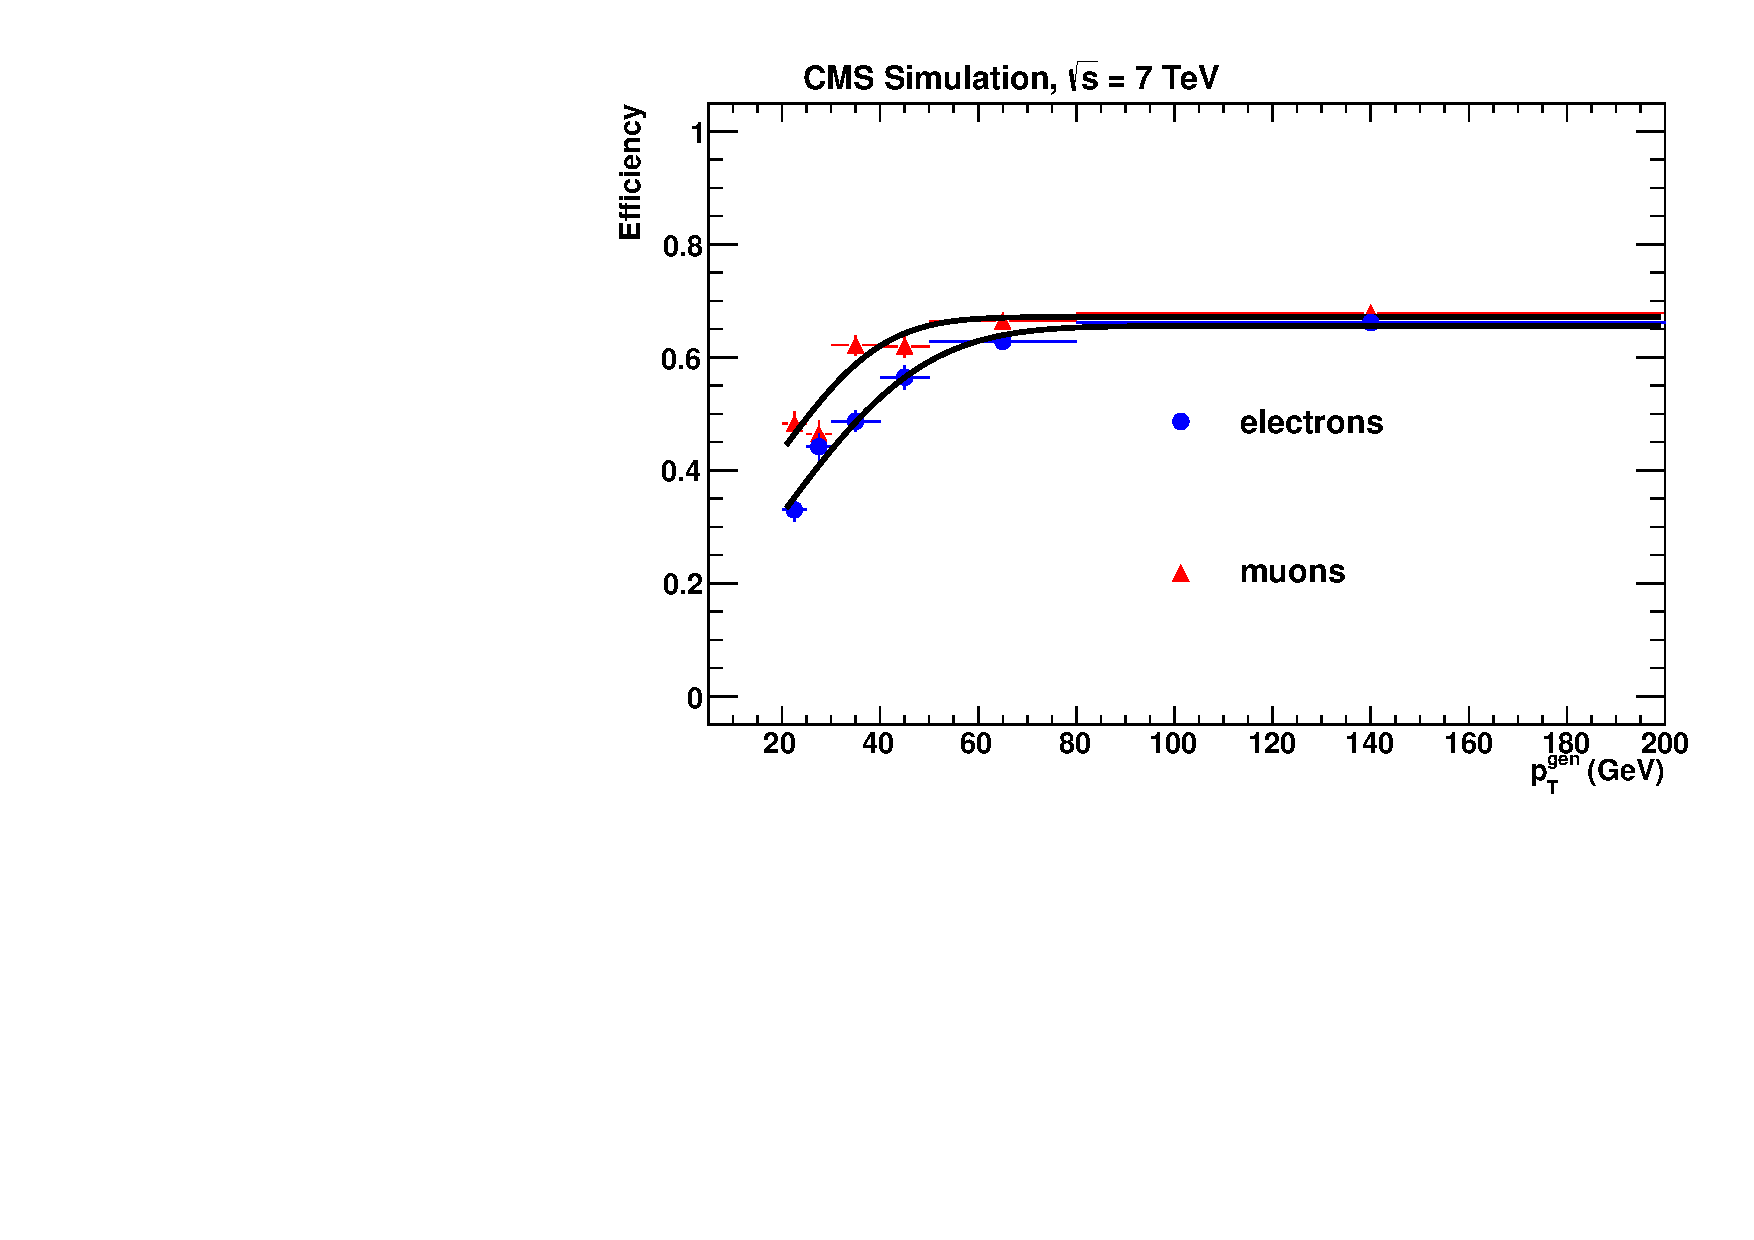
\includegraphics[width=0.7\linewidth]{figs/leptonEfficiency_lm6}
\caption{\label{fig:lepeffLM6}
Lepton selection efficiency as a function of \pt,
displayed for electrons and muons.
}
\end{center}
\end{figure}

%
The efficiency dependence can be parameterzied as a function of \pt\ as 
%
\begin{eqnarray}
\epsilon = \epsilon_{\rm \infty} {\rm erf}\left ( \frac{\pt - C}{\sigma} \right)
	+ \epsilon_C \left( 1.- {\rm erf}\left ( \frac{\pt - C}{\sigma} \right) \right),
\label{eq:lepeffFitF}
\end{eqnarray}
where $\epsilon_{\rm \infty}$ gives the value of the efficiency plateau at high momenta,
$C$ is equal to 20~\GeV,
$\epsilon_C$ gives the value of the efficiency at $\pt=C$,
and $\sigma$ describes how fast the transition region is.
The results of the fit for electrons and muons are summarized in Table~\ref{tab:lepeffLM6fit}.
%
\begin{table}[h]
\begin{center}
\caption{\label{tab:lepeffLM6fit} Results of the fit of the dependence in Fig.~\ref{fig:lepeffLM6}
to the function specified in Eq.~\ref{eq:lepeffFitF}.}
\begin{tabular}{l|cc}\hline\hline
Parameter		& Electrons		& Muons			\\ \hline
$\epsilon_{\infty}$	& $0.718\pm0.008$	& $0.757\pm0.006$	\\
$\epsilon_{C}$		& $0.498\pm0.021$	& $0.614\pm0.026$	\\
$\sigma$		& $25.8\pm4.0$		& $12.9\pm2.5$		\\
\hline\hline
\end{tabular}
\end{center}
\end{table}

%
%
\subsection{\met\ and $\Ht$ efficiency turn-on}
\label{sec:turnon}
Our selections on reconstructed jets begin with a requirement of at least two jets with $\pt>40~\GeV$.
Two such jets are present in approximately 95\% of the events in LM1 and LM6 with $\Ht^{\rm gen}>200~\GeV$ prior
to any additional requirement on colored partons at the generator level beyond the sum of \pt.
This represents the fraction of acceptance to two jets.
In the following we proceed with determining $\Ht$ and \met\ requirement with respect to 
events that have generator-level requirements on the leptons and colored particles as described in Section~\ref{sec:acceptance}.
%
The efficiency for an event to pass a given reconstructed \met\ ($\Ht$) threshold is shown in Fig.~\ref{fig:htmetThresh}
as a function of $\met^{\rm~gen}$ ($\Ht^{\rm gen}$) in events passing $\Ht^{\rm gen}>200~\GeV$ ($\met^{\rm~gen}>30~\GeV$).
Due to the rather small fraction of events in LM6 simulation having low \Ht\ activity, the \Ht\ curves are made with LM1.
Results of the fits of these curves to $0.5 \epsilon_{\infty} \{{\rm erf}[(x - x_{1/2})/\sigma] + 1\}$ are summarized
in Table~\ref{tab:htmetThresh}.
Neither the \met\ nor \Ht\ curves show a significant bias in the position of the point with half the plateau efficiency ($x_{1/2}$).
The inefficiency at the plateau is essentially negligible.
The width of the threshold $\sigma$ increases with the value of the cut.
%
\begin{figure}[h]
\begin{center}
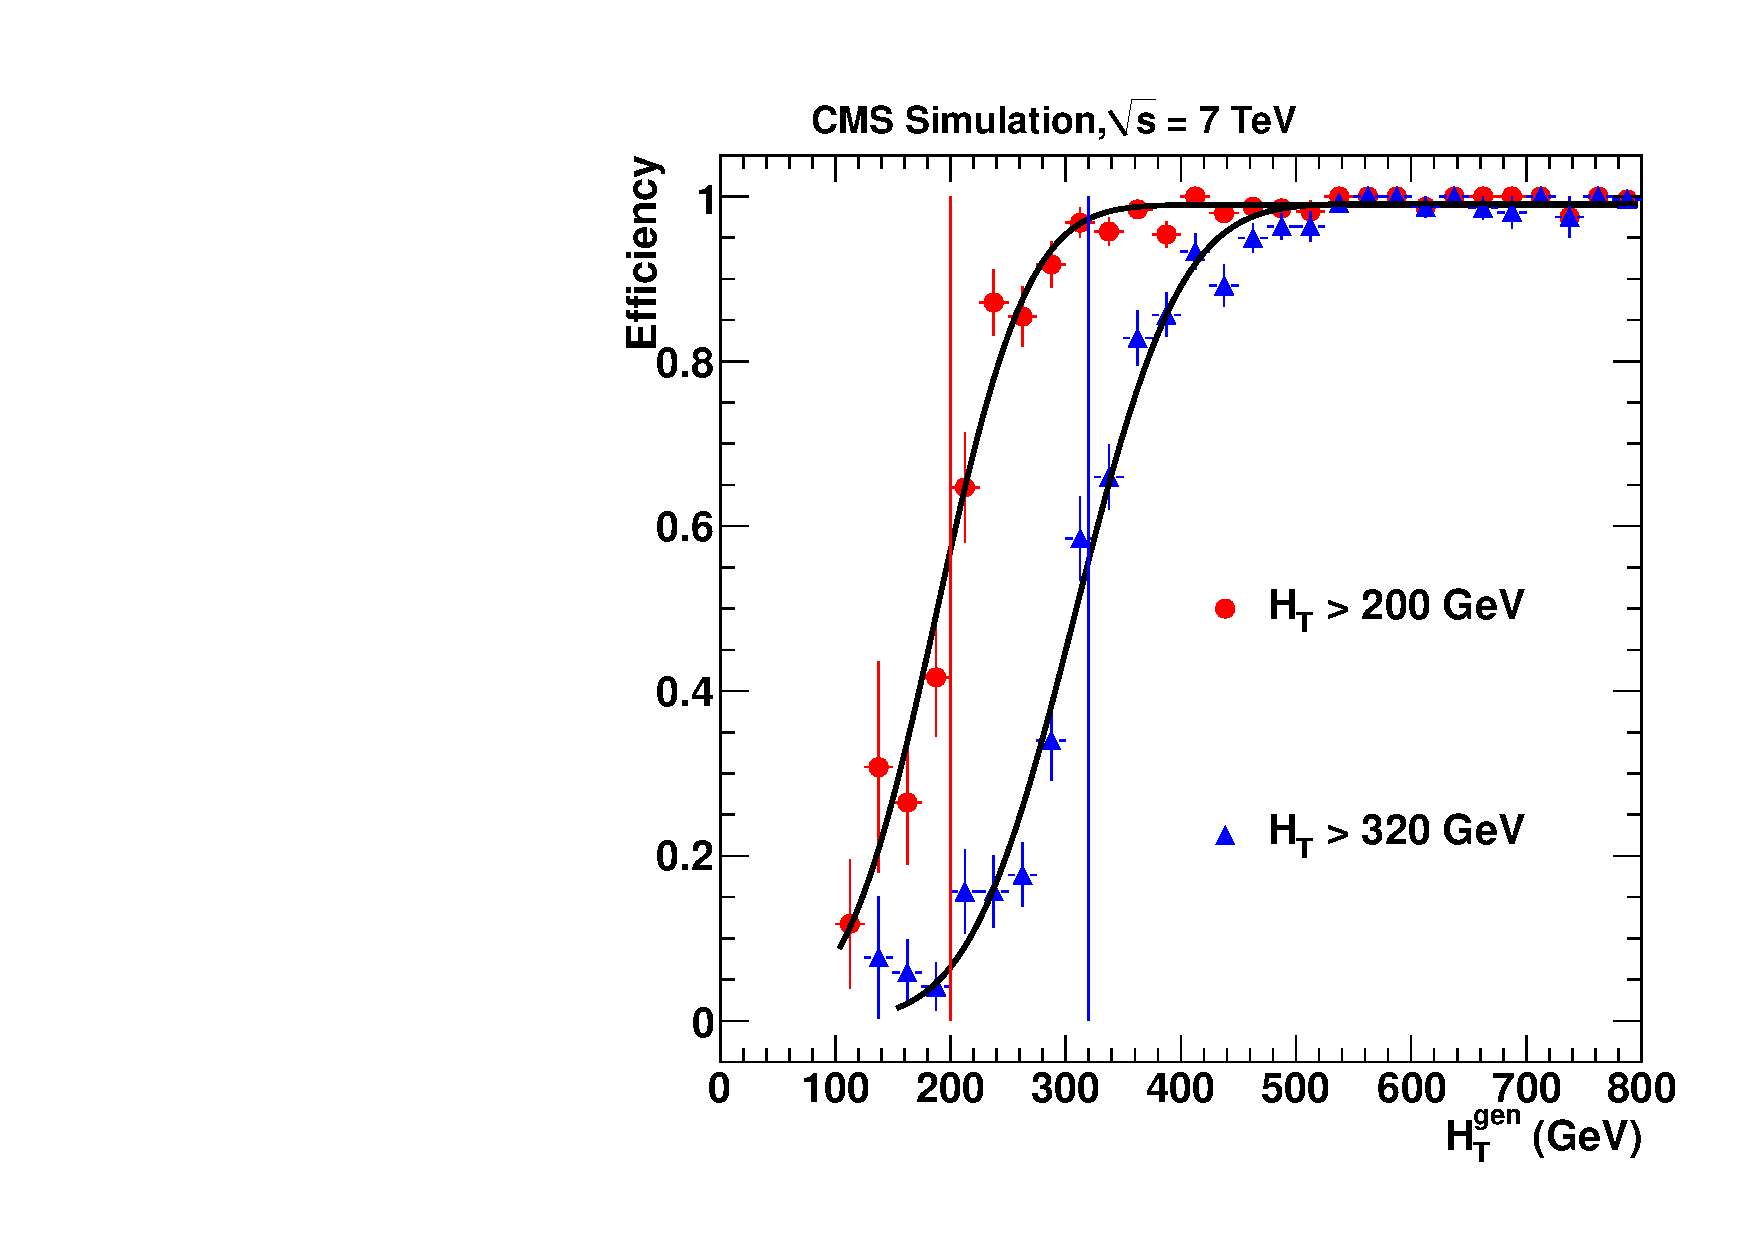
\includegraphics[width=0.48\linewidth]{figs/HTturnOnCurve_lm1}
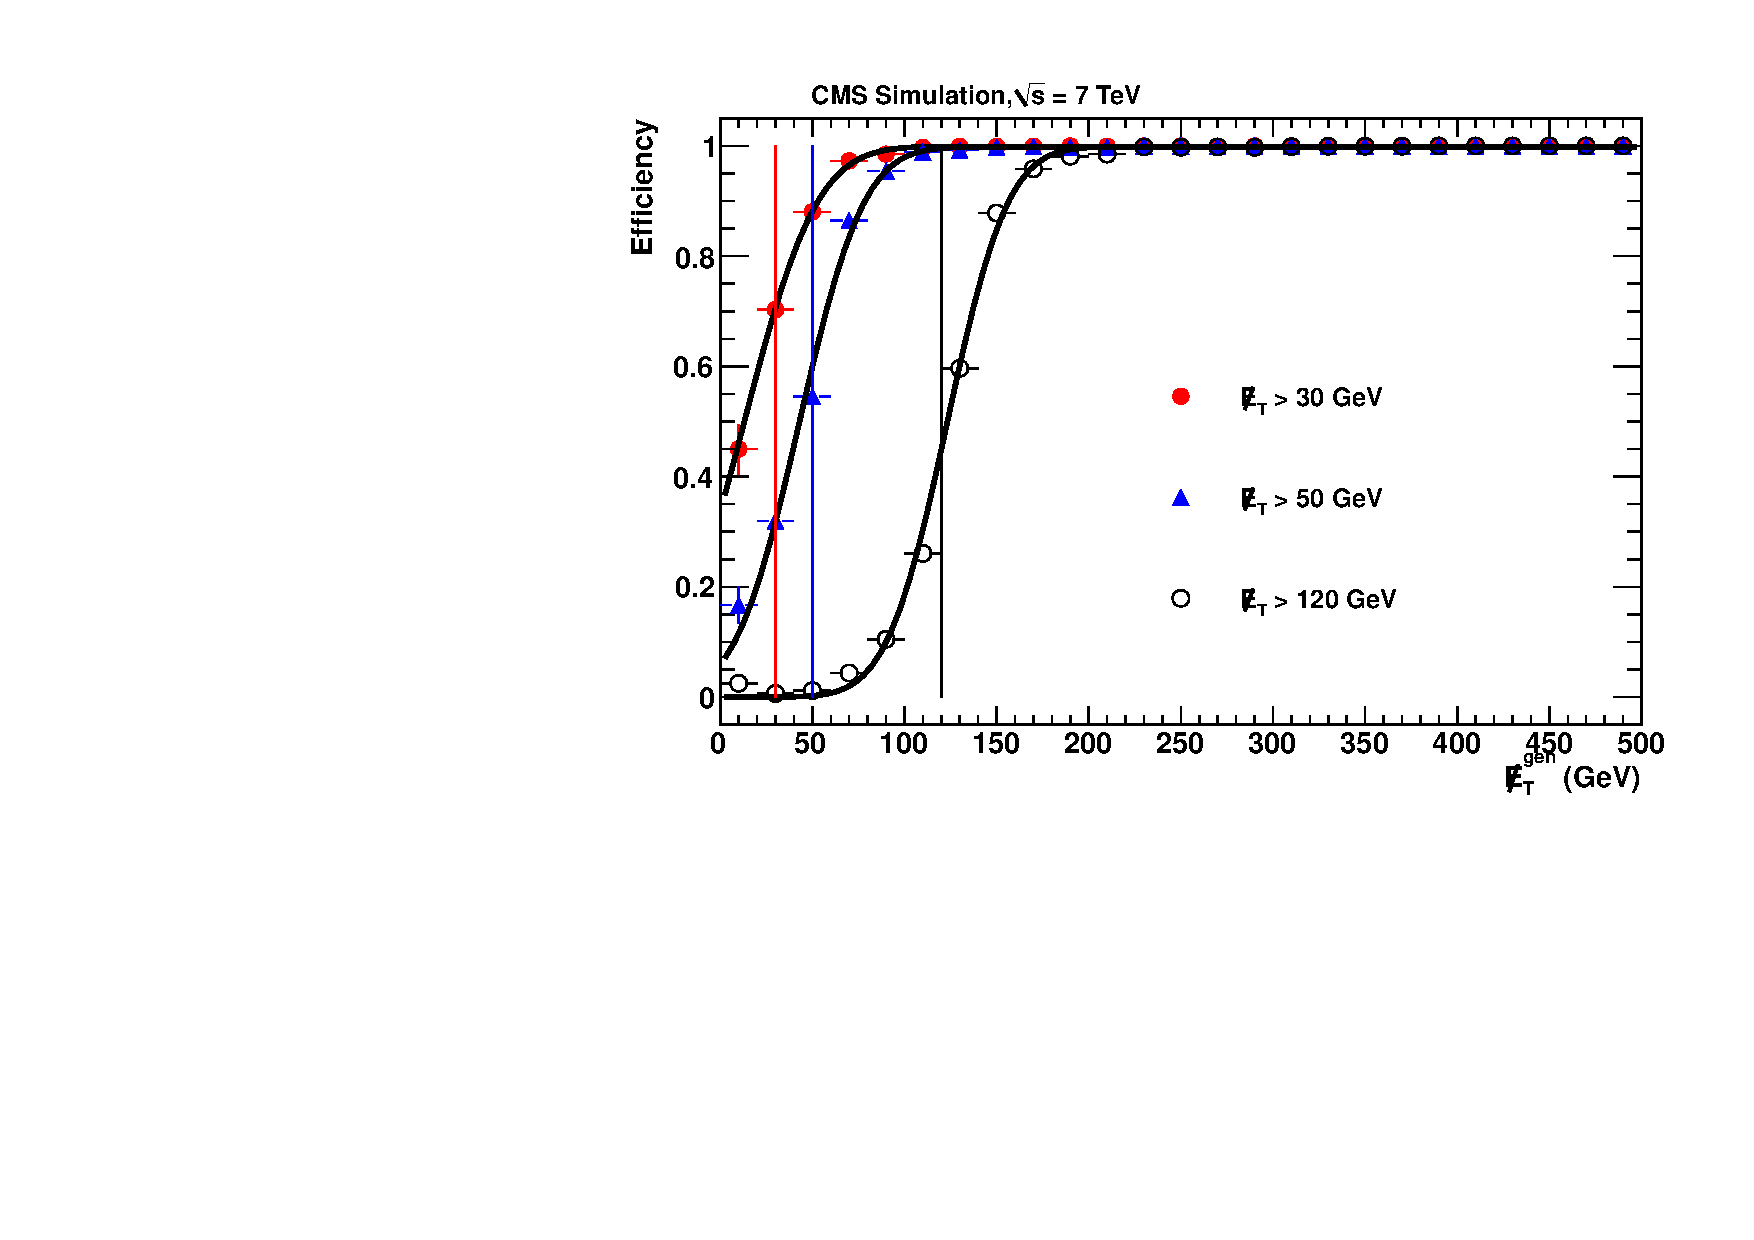
\includegraphics[width=0.48\linewidth]{figs/metTurnOnCurve_lm6}
\caption{\label{fig:htmetThresh}
Efficiency for an event to pass a given reconstructed \met\ ($\Ht$) threshold 
as a function of $\met^{\rm~gen}$ ($\Ht^{\rm gen}$).
The curves are shown for \met\ thresholds of 30, 50, and 120~\GeV;
the thresholds for \Ht\ are 200, 320, and 440~\GeV.
}
\end{center}
\end{figure}
%
%
\begin{table}[h]
\begin{center}
\caption{\label{tab:htmetThresh} Results of the fit of the dependence in Fig.~\ref{fig:htmetThresh}
to $0.5 \epsilon_{\infty} \{{\rm erf}[(x - x_{1/2})/\sigma] + 1\}$.}
\begin{tabular}{l|ccc|ccc}\hline\hline
Parameter		& \multicolumn{3}{|c}{\Ht}			& \multicolumn{3}{|c}{\met}			\\ 
			&	$>200~\GeV$	&	$>320~\GeV$	& $> 440~\GeV$		& $>30~\GeV$		& $>50~\GeV$		& $>120~\GeV$	\\ \hline
$\epsilon_{\infty}$	& $0.990\pm0.002$	& $0.992\pm0.003$	& $0.986\pm0.005$	& $0.999\pm0.001$	& $0.999\pm0.001$	& $0.999\pm0.001$ \\
$x_{1/2}$,~\GeV		& $187.8\pm 5.5$	& $308.4\pm 3.3$	& $428.8\pm3.2$		& $13.1\pm2.4$		& $43.0\pm1.1$		& $123.3\pm 0.5$  \\
$\sigma$,~\GeV		& $88.3\pm9.8$		& $102.0\pm6.2$		& $120.3\pm6.1$		& $44.0\pm2.8$		& $38.9\pm1.6$		& $36.6\pm0.9$	\\
\hline\hline
\end{tabular}
\end{center}
\end{table}


\subsection{Jet b-tagging efficiency}
\label{sec:btagEff}
The b-jet tagging efficiency is defined for b-quarks passing $|\eta|< 2.5$ and matching to a reconstructed jet.
A fraction of these b-quark that match to a b-tagged jet is the b-jet tagging efficiency.
It shown in Fig.~\ref{fig:btagEff} as a function of the b-quark \pt.
For b-quarks of $|\eta| < 2.5$, the b-jet tagging efficiency as a function of \pt
can be parametrized as 
\begin{itemize}
\item \pt $<$ 90 GeV:~~~~~~~~~~~~~~~~$\epsilon = SF \cdot [p0 \cdot (p_t-90~{\rm GeV}) + p1]$
\item 90 GeV $<$ \pt $<$ 170 GeV:~~~~$\epsilon = SF \cdot p1$
\item \pt $>$ 170 GeV:~~~~~~~~~~~~~~$\epsilon = SF \cdot [p2 \cdot (p_t-170~{\rm GeV}) + p1]$
\end{itemize}

\noindent where the parameters $p0$, $p1$, and $p2$ are given in Figure~\ref{fig:btagEff}
and $SF$ is the data-Monte Carlo scale factor: $SF$ = 0.96 with a 
4 (15)\% uncertainty for jets with $\pt<240 (>240)~\GeV$ (see 
Section~\ref{sec:bjetSF}). 
% {\bf Make sure that the parametrization is correct.}

\begin{figure}[h]
\begin{center}
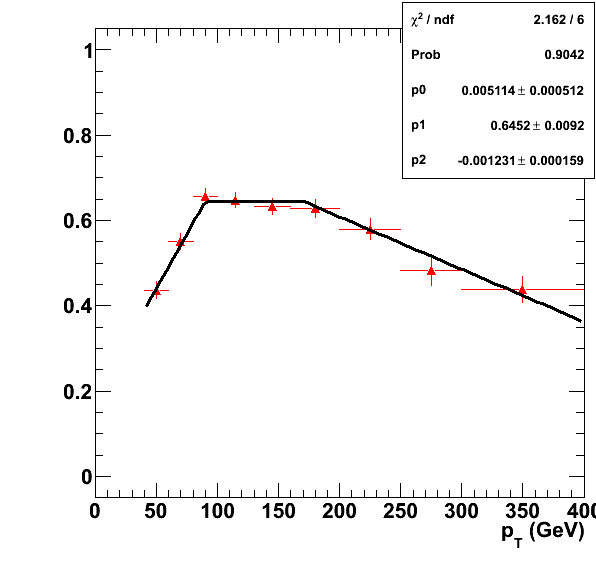
\includegraphics[width=0.48\linewidth]{figs/lm6_btagEffWithCurve.png}
\caption{\label{fig:btagEff}
B-jet tagging efficiency as a function of the matching b-quark \pt in LM6 SUSY MC.
}
\end{center}
\end{figure}

\section{Data - Monte Carlo Scale Factors and their Uncertainties}
\label{sec:SF}

\subsection{Data - Monte Carlo Scale Factor for Leptons}
\label{sec:tnp}

The efficiencies of the lepton isolation and identification requirements (including all quality requirements) 
are measured with the tag\&probe method in dilepton Z events using the full 2011 dataset.
The efficiency of the identification requirements is a property of the lepton itself and is directly applicable
 to the leptons in signal events.
The efficiency of the isolation requirement, however, is a strong function of all other (mainly hadronic)
activity in the event.
The following results are based on measurements using the full dataset and compared 
to simulation that is re-weighed to have a pile-up distribution comparable to that observed in data.

The electron selection efficiencies are measured in events passing 
the \verb=Ele17..._SC8_Mass30= and \\\verb=Ele17.._Ele8_Mass30= triggers,
which require one well-identified electron and one super-cluster or GSF electron with $\pt>8~\GeV$ forming a pair with a mass
above 30~\GeVcc.  
For higher $\pt$ electrons, the \verb=Ele32...SC_17= triggers are also used, 
which require one well identified electron and one super-cluster with $\pt >17~\GeV$.
In the tag\&probe analysis the electron tag is required to match to the well-identified electron 
from the trigger and also to pass all the electron requirements described in~\cite{ssnote2011}.
The probe electron is required to have
\begin{itemize}
\item $\pt>20~\GeV$, $|\eta|<2.4$, excluding the superclusters with $1.4442<|\eta|<1.566$.
\end{itemize}
The isolation efficiency is measured with the probes passing all electron selections , except for the 
trigger requirement and the isolation itself.
The identification efficiency is measured with probes passing the isolation requirement.
Results of the measurement are summarized in Table~\ref{tab:eleEffs}.
The contribution from the Z events is based on simple counting in the mass range of 86--96~\GeVc,
the MC contribution includes Wjet events to match the expected residual backgrounds in this mass window.
The following sources of systematic uncertainty are attributed to this measurement:
background contribution, selection of dielectron events, factorization of the isolation and ID parts.
The size of the background contribution can be estimated using MC alone
and also  tested in data with  the same-sign dielectron
events, which should represent the number of backgrounds reasonably well.
The effect of backgrounds on the measured efficiency is established to be approximately 
2\% for the combined identification
and isolation selection efficiency.
The narrow mass window used to count electron pairs introduces a bias of about 3\% 
to the measured efficiency
by rejecting failing probes that happen to have a worse resolution or a shift
in the measured momentum.
This bias is expected to approximately cancel in data and simulation.
We include a half of the 3\% as a source of systematics.
Based on simulation alone, the combined selection efficiency, measured with respect to the probe electron,
differs from the product of the components by approximately 1\% or less depending on the momentum range.
All of these effects combined give a systematic uncertainty on the total data-to-MC scale factor
in the lepton selection efficiencies of 2.5\% for $\pt>20~\GeV$.

\begin{table}[h]
\begin{center}
\begin{tabular}{c|c|ccc}
\hline\hline
& & 20 - 40 GeV & 40 GeV -  \\
\hline
				& MC			& 	0.9268 $\pm$ 0.0004 & 	0.9768 $\pm$ 0.0002 \\
ISO				& DATA			& 	0.9247 $\pm$ 0.0003 & 	0.9737 $\pm$ 0.0002 \\
				& DATA/MC		& 	0.9977 $\pm$ 0.0005 & 	0.9968 $\pm$ 0.0003 \\
\hline
				& MC			& 	0.8069 $\pm$ 0.0005 & 	0.8500 $\pm$ 0.0004 \\
ID				& DATA			& 	0.8005 $\pm$ 0.0005 & 	0.8343 $\pm$ 0.0004 \\
				& DATA/MC		& 	0.9921 $\pm$ 0.0008 & 	0.9815 $\pm$ 0.0006 \\
\hline
				& MC			& 	0.7478 $\pm$ 0.0005 & 	0.8303 $\pm$ 0.0004 \\
ID X ISO			& DATA			& 	0.7403 $\pm$ 0.0005 & 	0.8124 $\pm$ 0.0004 \\
				& DATA/MC		& 	0.9899 $\pm$ 0.0010 & 	0.9784 $\pm$ 0.0007 \\
\hline \hline
\hline
\end{tabular}
\caption{\label{tab:eleEffs}Electron isolation and identification efficiencies measured with the tag\&probe method.
The uncertainties are statistical only.}
\end{center}
\end{table}

The muon selection efficiencies are measured using events passing the double-muon trigger.
The tag muon is required to pass all of the muon selection requirements described in~\cite{ssnote2011}.
The probe muon is required to pass
\begin{itemize}
\item $\pt>20~\GeVc$;
\item $|\eta|<2.4$;
\item have both the global and the tracker muon types.
\end{itemize}
Both the  isolation and the identification efficiency are measured using probes failing only the requirement in question,
assuming the efficiencies factorize.
Results of the muon identification and isolation efficiency measurements are presented in Table~\ref{tab:muEffs}.
As expected, the identification efficiency for muons measured in data and in MC agree well,
while there is some discrepancy for the isolation efficiency.
Similar sources of systematic uncertainty are considered here as those considered for electrons.
Most of the reconstructed (probe) muons are real muons and the measurement of the identification efficiency
is not affected significantly by backgrounds.
With the tighter mass window used here to select events,
 the backgrounds are estimated to be small.
This narrow mass window, however, introduces a bias of about 1.5\% 
to the measured efficiency
by rejecting failing probes that happen to have a worse resolution or a shift
in the measured momentum.
This bias is expected to approximately cancel in data and simulation.
We include a half of the 1.5\% as a source of systematics.
We assign a systematic uncertainty of 1\% on the identification and isolation efficiency measurement  
from a comparison between the simple counting of Z events and fitting the mass shape to a gaussian signal and an 
exponential background component.
Based on studies in MC events, we find that the isolation and the identification efficiencies
 factorize near-perfectly and do not assign any additional systematic uncertainty.
The total systematic uncertainty on the muon efficiency measurement in 
data, simply covering the full momentum range, is 2\%.


\begin{table}[h]
\begin{center}
\begin{tabular}{c|c|cc}
\hline\hline
& & 20 - 40 GeV & 40 GeV -  \\ 
\hline
				& MC			& 	0.9111 $\pm$ 0.0003& 	0.9747 $\pm$ 0.0002 \\
ISO				& DATA			& 	0.8969 $\pm$ 0.0003& 	0.9668 $\pm$ 0.0002 \\
				& DATA/MC		& 	0.9844 $\pm$ 0.0004& 	0.9919 $\pm$ 0.0002 \\
\hline
				& MC			& 	0.9710 $\pm$ 0.0002& 	0.9612 $\pm$ 0.0002 \\
ID				& DATA			& 	0.9666 $\pm$ 0.0002& 	0.9561 $\pm$ 0.0002 \\
				& DATA/MC		& 	0.9955 $\pm$ 0.0003& 	0.9947 $\pm$ 0.0003 \\
\hline
				& MC			& 	0.8847 $\pm$ 0.0003& 	0.9369 $\pm$ 0.0002 \\
ID X ISO			& DATA			& 	0.8669 $\pm$ 0.0003& 	0.9244 $\pm$ 0.0002 \\
				& DATA/MC		& 	0.9799 $\pm$ 0.0005& 	0.9866 $\pm$ 0.0003 \\
\hline \hline
\end{tabular}
\caption{\label{tab:muEffs}Muon isolation and identification efficiencies measured with the tag\&probe method.
The uncertainties are statistical only.}
\end{center}
\end{table}

The tag\&probe results in Tables~\ref{tab:eleEffs} and~\ref{tab:muEffs}
show that for leptons with $\pt>20~\GeV$ used in this analysis both the ID part and the isolation parts
 of the lepton selection are reproduced well by simulation, already within the systematic uncertainties
quoted above.
Application of this measurement based on Z events to the signal events incurs
an additional uncertainty due to potential mismodeling of the isolation requirement.
In agreement with Ref.~\cite{ssnote2011}, we assign a systematic uncertainty of 5\% 
due to modeling of the isolation efficiency for signal events.
Considering the small size of the difference between data and simulation reported in 
Tables~\ref{tab:eleEffs} and~\ref{tab:muEffs}, compared to the systematic uncertainty
applicable to the analysis,
we approximate the scale factor to be 1.0 for both simulated signal and backgrounds
and propagate the uncertainty described above to the relevant part of the analysis
(signal selections) described in Section~\ref{sec:systematic}.

\subsection{Data - Monte Carlo Scale Factor for b-jets}
\label{sec:bjetSF}
We apply an average scale factor of 0.96 measured using \ttbar\ events
for the SSVHEM tagger~\cite{BTV11003}.
The uncertainty on the scale factor is 4 (15)\% for jets with $\pt<240 (>240)~\GeV$,
as recommended by the b-tagging POG~\cite{btvSyst} and apply
it to the analysis as described in Section~\ref{sec:systematic}.
\section{Background Contributions}
\label{sec:bkgds}

We are following the same strategy in estimating the background contributions as in
the pre-tagged sample analysis~\cite{ssnote2011}.
Contributions with genuine same-sign isolated lepton pairs are estimated from simulation,
while the contributions from leptons arising from jets (fakes) and from genuine opposite-sign pairs
with a lepton charge misreconstruction (charge flips) are measured in data using control data samples.
The data-driven estimates are described in the next section.
In addition, as a reference, we are using all relevant available simulated samples to get a feeling of the expected yields
from simulation alone.
As will be shown later in Section~\ref{sec:yields}, contributions with genuine same-sign isolated dileptons
are comparable to those estimated from events with fake leptons, while the predictions from charge flips are
relatively low.
These findings are in a fair agreement with direct estimates from simulation.


We use MC to estimate contributions from the following SM production processes with genuine same-sign isolated dileptons:
\begin{itemize}
\item $qqW^\pm W^\pm, WWW, WWZ, WZZ, ZZZ, WW\gamma, t\bar{t}W, t\bar{t}Z, t\bar{t}\gamma$ and double parton $W^\pm W^\pm$ with two real leptons in the final state.
\item $WZ$, $W\gamma^\star$ ($0.25~\GeV < m_{\gamma^\star}<12~\GeV$), and $ZZ$ with two real leptons in the final state.
\item $W\gamma$ with one real lepton and a photon conversion. 
This background is a priori not estimated by the fake rate method
because the photon is generally isolated. 
%In practice, this background is completely negligible.
\end{itemize}
Details on the sameples used and the corresponding cross sections can be found in Ref.~\cite{ssnote2011}.
As in the pre-tagged sample analysis, we are assigning a 50\% uncertainty to the expected
number of events from these samples.
\section{Data Driven Background Estimation Methods}
\label{sec:datadriven}

We have developed two data-driven methods to 
estimate the two potentially dominant backgrounds.
The first method provides an estimate of the number of events with fake leptons (jets misidentified as leptons).
The second method is used to estimate the number of genuine leptons reconstructed with an incorrect charge sign.

\subsection{Data Driven prediction for fake lepton backgrounds}
\label{sec:fakes}

We predict the background from fake leptons using the technique previously implemented in 2010 data analysis
and documented in~\cite{frmethod}.
The idea is to count the number of events for which one lepton passes all final selections and a second lepton
fails the nominal requirements but passes a looser set of requirements. 
We refer to the former lepton as a "numerator" lepton ($n$),
and the latter a "non-numerator" (denominator and not numerator, or $\bar{n}$).
The denominator objects are also referred to as fakeable objects (FO).
The ratio of "numerator" to "denominator" objects is called a "fake rate",
 FR (also known as tight-to-loose ratio, TL).  
A fake rate function is measured in an independent data sample of multijet events.
This fake rate function is measured in bins of lepton $\pt$ and $|\eta |$,
separately for electrons and muons. 

The numerator selections are detailed in Section~\ref{sec:eventSel}. 
The denominator selections are described below, specifying only looser selections.

Muon denominator definition is to relax the following muon requirements from
Section~\ref{sec:eventSel}:
\begin{itemize}
\item $\chi^2$/ndof of global fit $<$ 50 (was $<$ 10);
\item transverse impact parameter with respect to the selected vertex is
$<$ 2 mm (was $<$ 200 $\mu$m);
\item $Iso$ is set to be $Iso < 0.4$  (was $<$ 0.1).
\end{itemize}

Electron denominator definition is to relax the following electron requirements from
Section~\ref{sec:eventSel}:
\begin{itemize}
\item the impact parameter cut is removed (was $<$ 200 $\mu$m);
\item $Iso$ is set to be $Iso < 0.6$ (was $<0.10$).
\end{itemize}
This is analogous to the V3 denominator in~\cite{frmethod} used for our previous analysis.

We thus use an extrapolation  in isolation (and impact parameter) to estimate the fake lepton backgrounds 
in both electrons and muons.
This choice is driven by the expectation that the selected events with fake leptons are dominated by
heavy flavor jets, in which the lepton candidate is predominantly a real lepton from b/c-quark semileptonic decays.
Relaxed isolation and impact parameter selections are then expected to roughly keep the same sample
composition in events with denominator leptons.

Samples of multijet (inclusive QCD) events in data are selected among events with a single lepton trigger present.
The samples and the triggers used in this measurement are listed in Section~\ref{sec:datasets}.
Since essentially all of the dilepton analysis events are collected on dilepton-triggered events, the
most appropriate choice for the FR measurement is to use  triggers based on the same (or almost the same) 
single-object triggers as the signal selection dilepton triggers.
The single-lepton triggered events are required to have an electron or a muon passing the denominator
requirements described above.
These events are further pruned of the contamination from the electroweak processes with W or Z production.
The W events are suppressed by a requirement that \met is below 20~GeV and the transverse mass $M_T < 25$~GeV.
The Z events are initially suppressed
by removing dielectron and dimuon events with another lepton matching 
the fakeable object and forming a pair with an invariant mass within the 71 to 111~GeV range
(events are removed only with  dileptons with both $\pt>20$~GeV and the other lepton
 passing a looser ID and isolation selection of the early $t\bar{t}$ analysis~\cite{frmethod}).
Further stringent suppression of remaining Z events is achieved by vetoing events satisfying the following conditions,
\begin{itemize}
\item for electrons:
\begin{itemize}
  \item other fakeable objects with $\pt>10~\GeV$ are present;
  \item there is a GSF track making a pair with the fakeable object and an invariant mass of 76 -- 106~GeV;
  \item the away jet has an EM-fraction higher than 0.8. 
\end{itemize}
\item for muons:
\begin{itemize}
  \item other fakeable objects with $\pt>10~\GeV$ are present;
  \item there is another muon (no ID requirement) with $\pt>10~\GeV$ making a pair with the fakeable object with an invariant mass of 76 -- 106~GeV;
  \item there is another muon (no ID requirement) with $\pt>10~\GeV$ making a pair with the fakeable object with an invariant
  mass between 8 and 12~GeV to additionally suppress Upsilon production contribution.
\end{itemize}
\end{itemize}

We repeat all the studies performed with 2010 data, as documented in~\cite{frmethod}.
These include 
\begin{itemize}
\item extraction of the fake rates in simulation and data;
\item closure tests on W+jet, \ttbar, and double-fake QCD events;
\item measurement of the fake-rate dependence on the {\em opposite-side} jet \pt,
	as a measure of the dependence on the progenitor parton momentum;
\item estimates of the residual W+jet and Z contamination in the sample;
\item comparison with the fake rate measured in events with enhanced heavy flavor
	contribution using b-tagging (the variation observed here is up to about 20\% for electrons and
	muons in both simulation and data).
\end{itemize}
We arrive to essentially the same conclusions on the performance of the fake-rate method
as we did in the past.
In particular, we find that the method works reasonably well, still with a systematic
uncertainty of about 50\%.
In the following we summarize the measurement of the fake rate and provide several highlights
of the studies with the current dataset.

The nominal fake rates are measured requiring an "opposite side" jet with $\pt>40~\GeV$, 
separated by $\Delta R > 1.0$ from the FO.
The electron fake rates are measured separately for triggers with an isolation requirement and
for triggers without any isolation requirement on the electron.
Results of the measurement are summarized in Tables~\ref{tab:frelectronTCaloIso},~\ref{tab:frelectronTNoIso} and ~\ref{tab:frelectronTCaloIsoTrkIso}
for the case with calorimeter, without, and with calorimeter and tracker isolation requirements, respectively.
The muon fake rates are measured using all single-muon triggers described in Section~\ref{sec:datasets}.
The measurement is summarized in Table~\ref{tab:frmuon}.


\begin{table}[h]
\begin{center}
\begin{tabular}{c|ccccc}
\hline
\backslashbox{$|\eta|$}{$p_T$} & 10.000 -- 15.000 & 15.000 -- 20.000 & 20.000 -- 25.000 & 25.000 -- 35.000 & 35.000 -- 55.000 \\ \hline\hline
0.000 -- 1.000 & 0.1985 $\pm$ 0.0141 & 0.1535 $\pm$ 0.0177 & 0.1260 $\pm$ 0.0212 & 0.1567 $\pm$ 0.0247 & 0.2198 $\pm$ 0.0434 \\ \hline
1.000 -- 1.479 & 0.1951 $\pm$ 0.0253 & 0.1867 $\pm$ 0.0318 & 0.1870 $\pm$ 0.0352 & 0.1800 $\pm$ 0.0384 & 0.3333 $\pm$ 0.0624 \\ \hline
1.479 -- 2.000 & 0.1880 $\pm$ 0.0339 & 0.1696 $\pm$ 0.0355 & 0.1481 $\pm$ 0.0279 & 0.1548 $\pm$ 0.0279 & 0.2596 $\pm$ 0.0430 \\ \hline
2.000 -- 2.500 & 0.2583 $\pm$ 0.0356 & 0.3084 $\pm$ 0.0446 & 0.1797 $\pm$ 0.0339 & 0.2836 $\pm$ 0.0389 & 0.3191 $\pm$ 0.0481 \\ \hline
\end{tabular}
\caption{\label{tab:frelectronTNoIso}Electron fake rate measured in bins of the electron candidate \pt\ and $\eta$
for electrons collected using triggers without isolation requirements.}
\end{center}
\end{table}

\begin{table}[htb]
\begin{center}
\begin{tabular}{c|ccccc}
\hline
\backslashbox{$|\eta|$}{$p_T$} & 10.000 -- 15.000 & 15.000 -- 20.000 & 20.000 -- 25.000 & 25.000 -- 35.000 & 35.000 -- 55.000 \\ \hline\hline
0.000 -- 1.000 & 0.2773 $\pm$ 0.0072 & 0.1784 $\pm$ 0.0072 & 0.1759 $\pm$ 0.0079 & 0.1789 $\pm$ 0.0084 & 0.2583 $\pm$ 0.0148 \\ \hline
1.000 -- 1.479 & 0.2749 $\pm$ 0.0121 & 0.2177 $\pm$ 0.0132 & 0.1977 $\pm$ 0.0115 & 0.1924 $\pm$ 0.0117 & 0.3026 $\pm$ 0.0197 \\ \hline
1.479 -- 2.000 & 0.2415 $\pm$ 0.0152 & 0.1806 $\pm$ 0.0137 & 0.1871 $\pm$ 0.0099 & 0.1916 $\pm$ 0.0095 & 0.2379 $\pm$ 0.0135 \\ \hline
2.000 -- 2.500 & 0.2827 $\pm$ 0.0146 & 0.2607 $\pm$ 0.0156 & 0.2420 $\pm$ 0.0119 & 0.2561 $\pm$ 0.0116 & 0.3225 $\pm$ 0.0154 \\ \hline
\end{tabular}
\caption{\label{tab:frelectronTCaloIso}Electron fake rate measured in bins of the electron candidate \pt\ and $\eta$
for electrons collected using triggers with a calorimeter isolation requirement.}
\end{center}
\end{table}

\begin{table}[htb]
\begin{center}
\begin{tabular}{c|ccccc}
\hline
\backslashbox{$|\eta|$}{$p_T$} & 10.000 -- 15.000 & 15.000 -- 20.000 & 20.000 -- 25.000 & 25.000 -- 35.000 & 35.000 -- 55.000 \\ \hline\hline
0.000 -- 1.000 & 0.3783 $\pm$ 0.0218 & 0.2932 $\pm$ 0.0279 & 0.2365 $\pm$ 0.0298 & 0.2713 $\pm$ 0.0324 & 0.3690 $\pm$ 0.0527 \\ \hline
1.000 -- 1.479 & 0.3556 $\pm$ 0.0357 & 0.3617 $\pm$ 0.0496 & 0.2364 $\pm$ 0.0405 & 0.2353 $\pm$ 0.0460 & 0.4667 $\pm$ 0.0644 \\ \hline
1.479 -- 2.000 & 0.2326 $\pm$ 0.0372 & 0.1638 $\pm$ 0.0344 & 0.2000 $\pm$ 0.0332 & 0.2260 $\pm$ 0.0314 & 0.2793 $\pm$ 0.0426 \\ \hline
2.000 -- 2.500 & 0.3357 $\pm$ 0.0399 & 0.2736 $\pm$ 0.0433 & 0.2362 $\pm$ 0.0377 & 0.2681 $\pm$ 0.0377 & 0.3645 $\pm$ 0.0465 \\ \hline
\end{tabular}
\caption{\label{tab:frelectronTCaloIsoTrkIso}Electron fake rate measured in bins of the electron candidate \pt\ and $\eta$
for electrons collected using triggers with calorimeter and tracker isolation requirements.}
\end{center}
\end{table}

\begin{table}[htb]
\begin{center}
\begin{tabular}{c|ccccc}
\hline
\backslashbox{$|\eta|$}{$p_T$} & 5.000 -- 10.000 & 10.000 -- 15.000 & 15.000 -- 20.000 & 20.000 -- 25.000 & 25.000 -- 35.000 \\ \hline\hline
0.000 -- 1.000 & 0.2760 $\pm$ 0.0028 & 0.2127 $\pm$ 0.0024 & 0.1808 $\pm$ 0.0032 & 0.1541 $\pm$ 0.0043 & 0.1441 $\pm$ 0.0009 \\ \hline
1.000 -- 1.479 & 0.3119 $\pm$ 0.0042 & 0.2527 $\pm$ 0.0036 & 0.2100 $\pm$ 0.0048 & 0.1820 $\pm$ 0.0067 & 0.1770 $\pm$ 0.0015 \\ \hline
1.479 -- 2.000 & 0.3340 $\pm$ 0.0042 & 0.2694 $\pm$ 0.0037 & 0.2238 $\pm$ 0.0049 & 0.2197 $\pm$ 0.0072 & 0.2018 $\pm$ 0.0016 \\ \hline
2.000 -- 2.500 & 0.3343 $\pm$ 0.0061 & 0.2741 $\pm$ 0.0054 & 0.2174 $\pm$ 0.0071 & 0.2012 $\pm$ 0.0108 & 0.2150 $\pm$ 0.0027 \\ \hline
\end{tabular}
\caption{\label{tab:frmuon}Muon fake rate measured in bins of the muon candidate \pt\ and $\eta$.
The uncertainties are statistical only.}
\end{center}
\end{table}

Figures~\ref{fig:frmuon}  and~\ref{fig:frelectron}  show the projection on $\pt$ and $|\eta|$ of these fake rates
for electrons and muons, respectively.
Electron fake rates measured for triggers with an isolation requirement are slightly higher than those
for triggers without an isolation requirement, as expected.
The difference, even though it's not very large, is significant enough and we treat fake rates for these triggers
separately.
The dependence of the fake rates on the away-jet momentum is also shown on these figures.

\begin{figure}[h]
\begin{center}
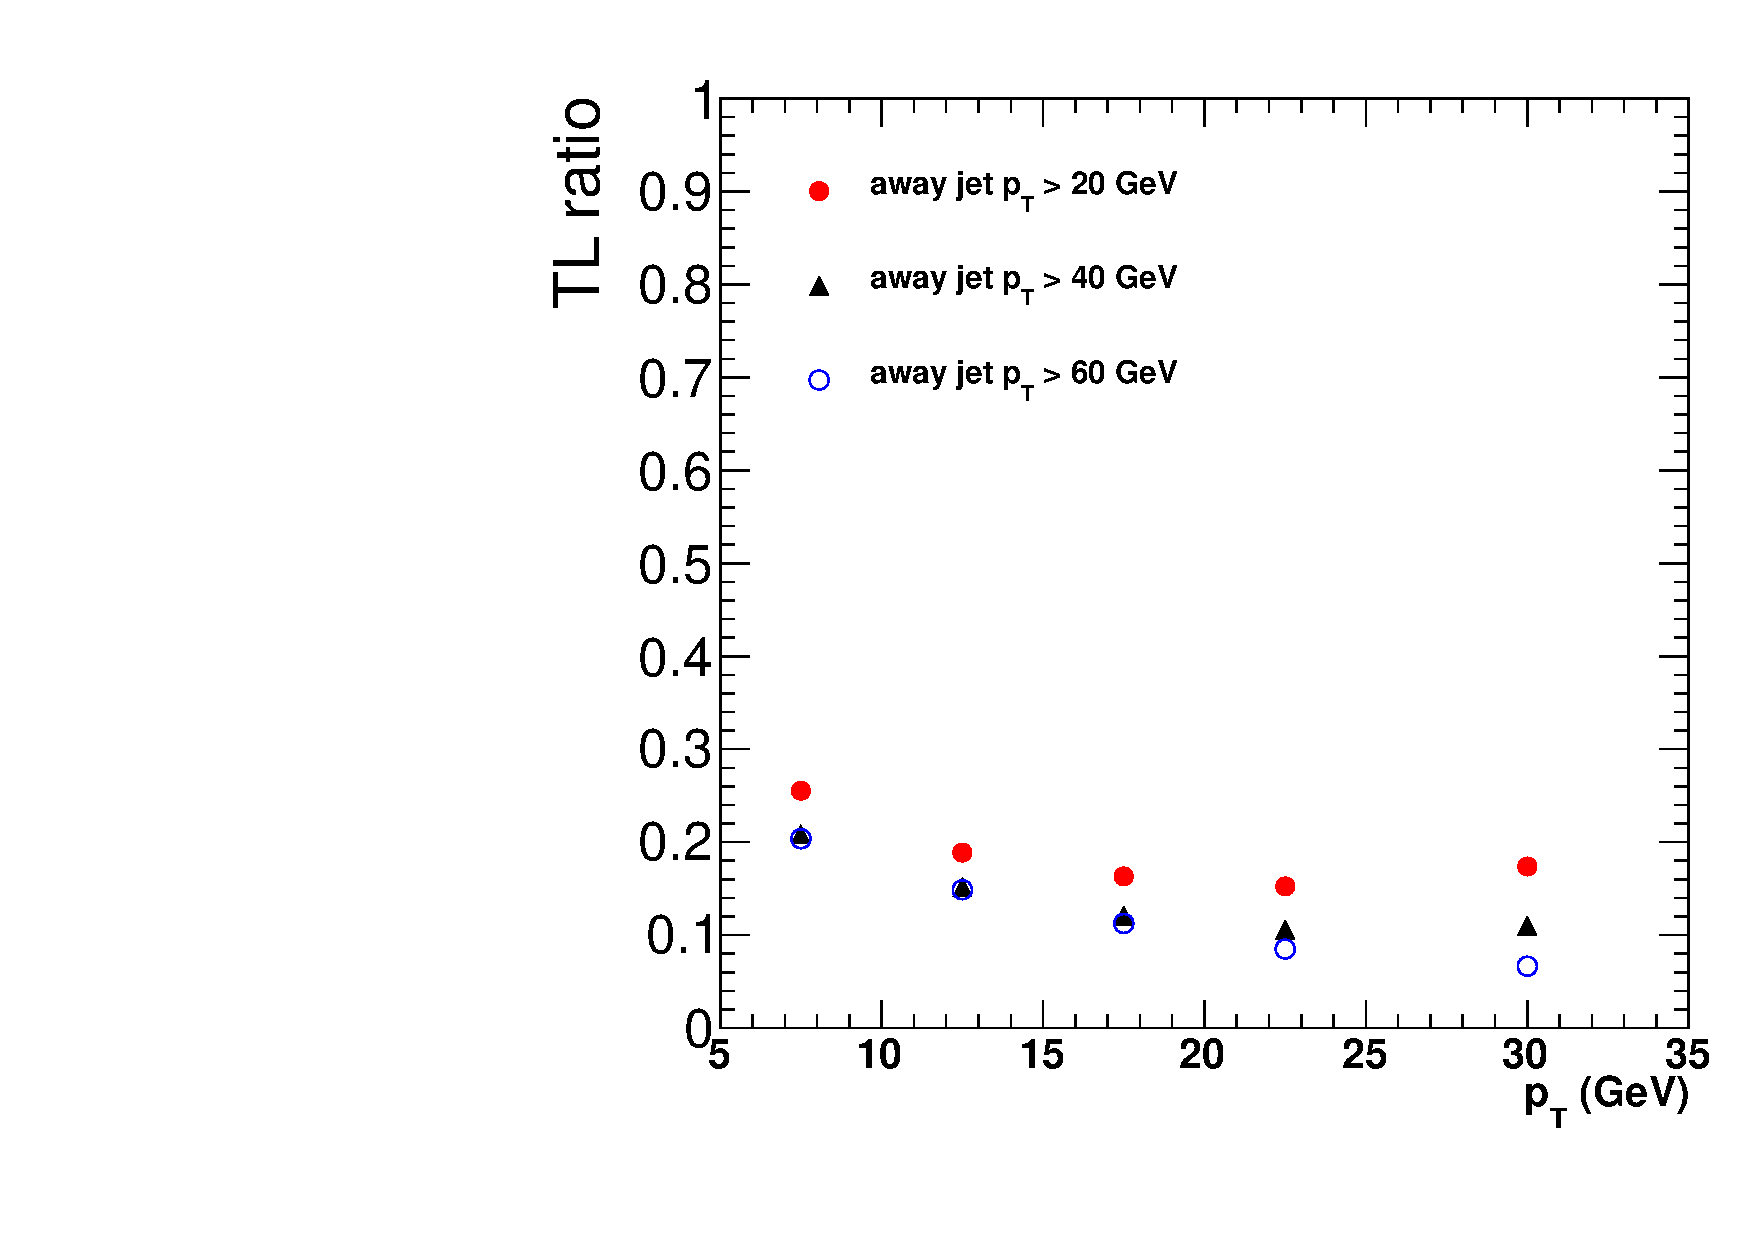
\includegraphics[width=0.48\linewidth]{figs/muFR_data_ptProj}
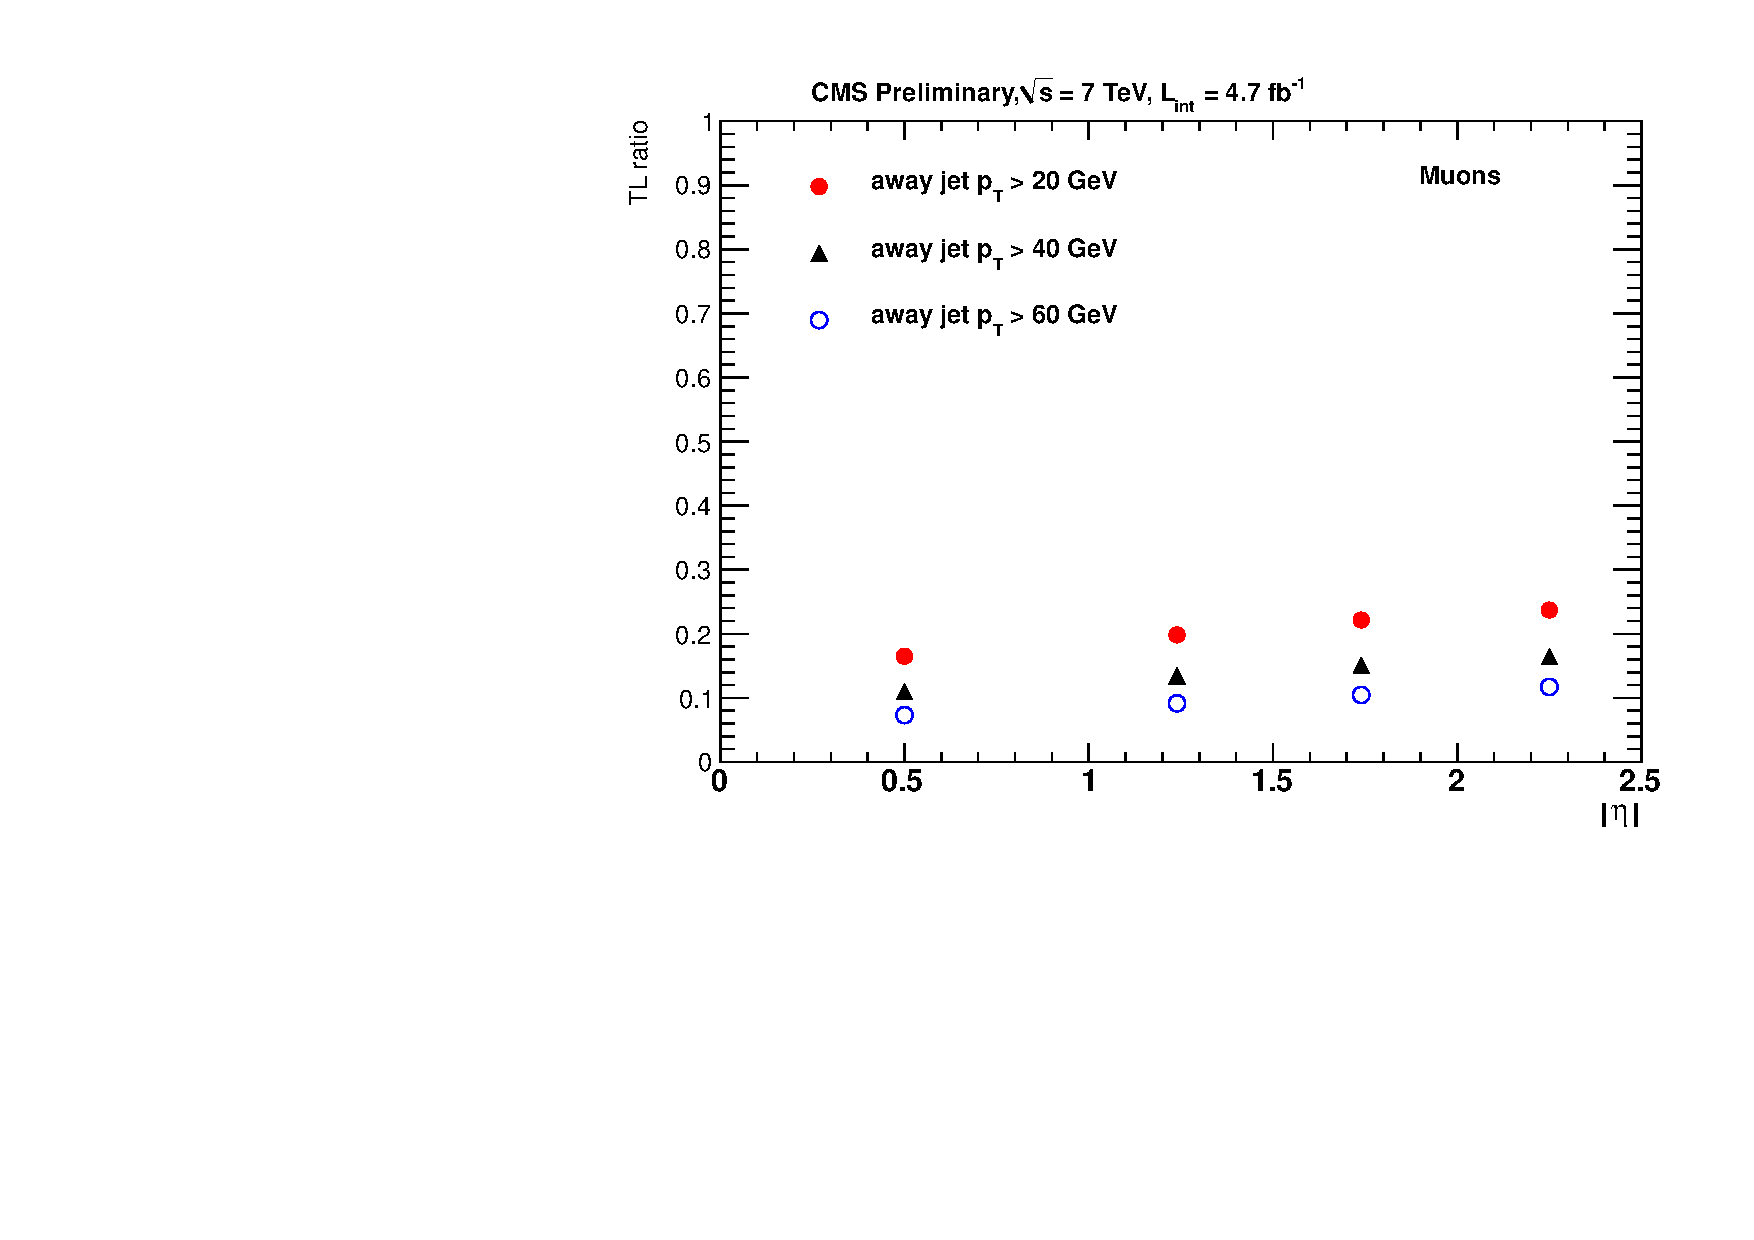
\includegraphics[width=0.48\linewidth]{figs/muFR_data_etaProj}
\caption{\label{fig:frmuon}Muon fake rate projected on $\pt$ (left) and $|\eta|$ (right).
The fake rates are shown separately for measurements  with a requirement for an away jet \pt\ 
to be above 20~\GeV\ (red circles), 40~\GeV\ (black circles), and 60~\GeV\ (blue circles).
}
\end{center}
\end{figure}

\begin{figure}[h]
\begin{center}
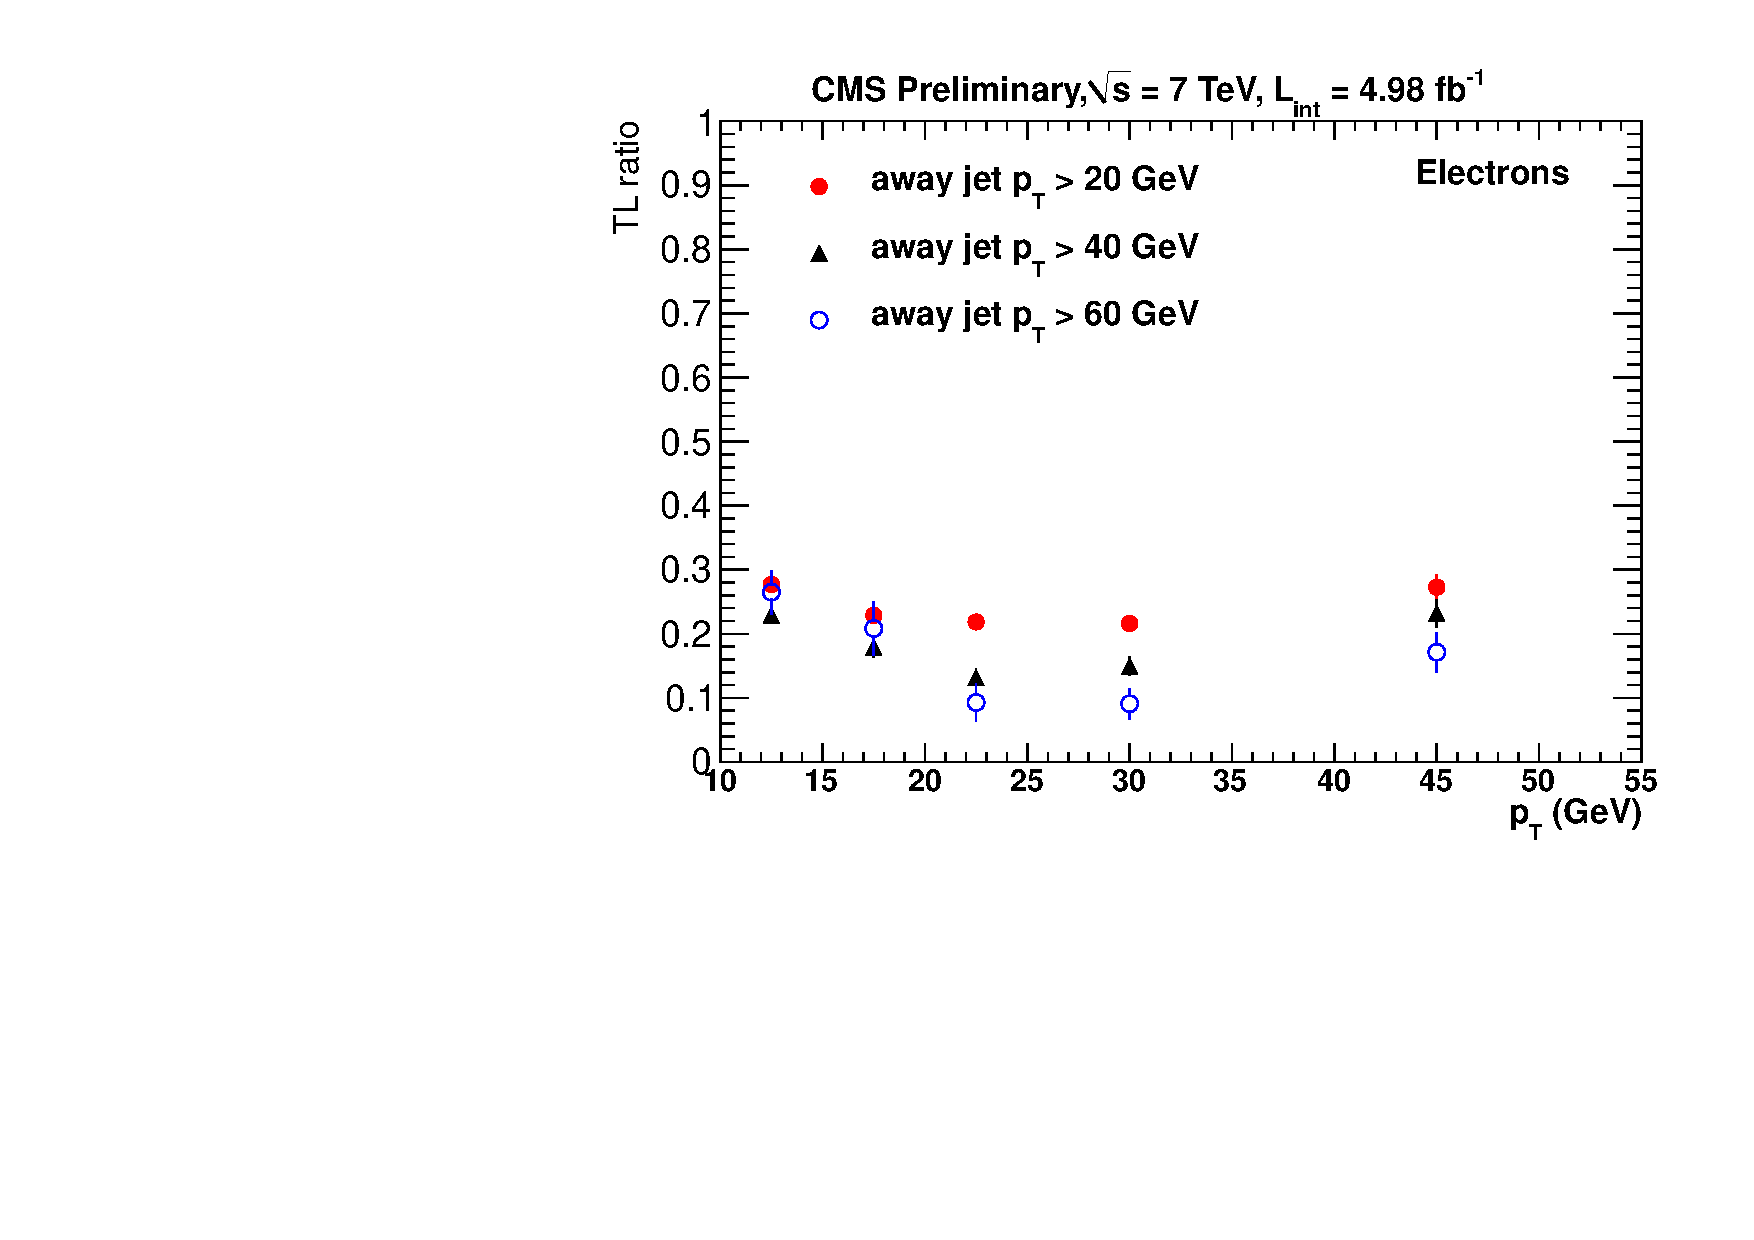
\includegraphics[width=0.48\linewidth]{figs/eleFRcaloIsoTrkIso_data_ptProj}
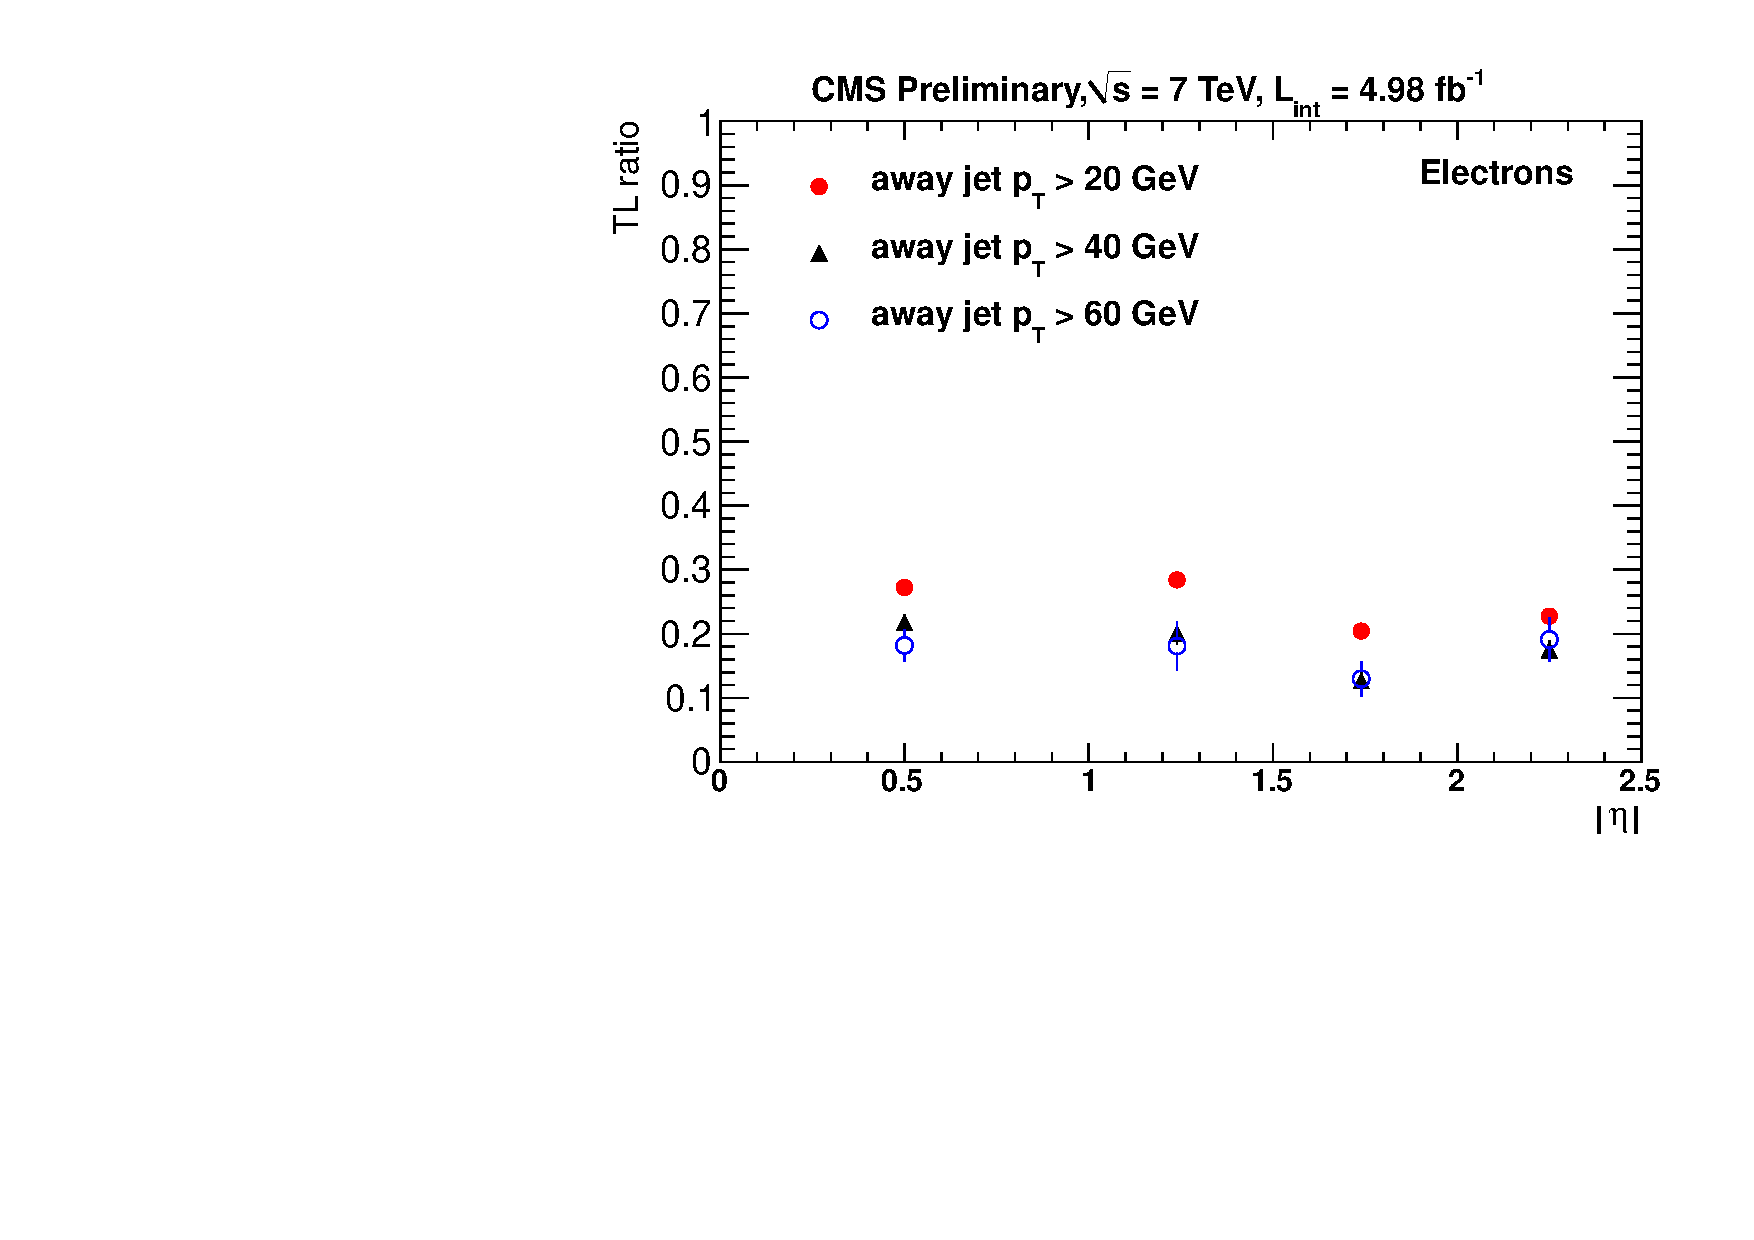
\includegraphics[width=0.48\linewidth]{figs/eleFRcaloIsoTrkIso_data_etaProj}\\
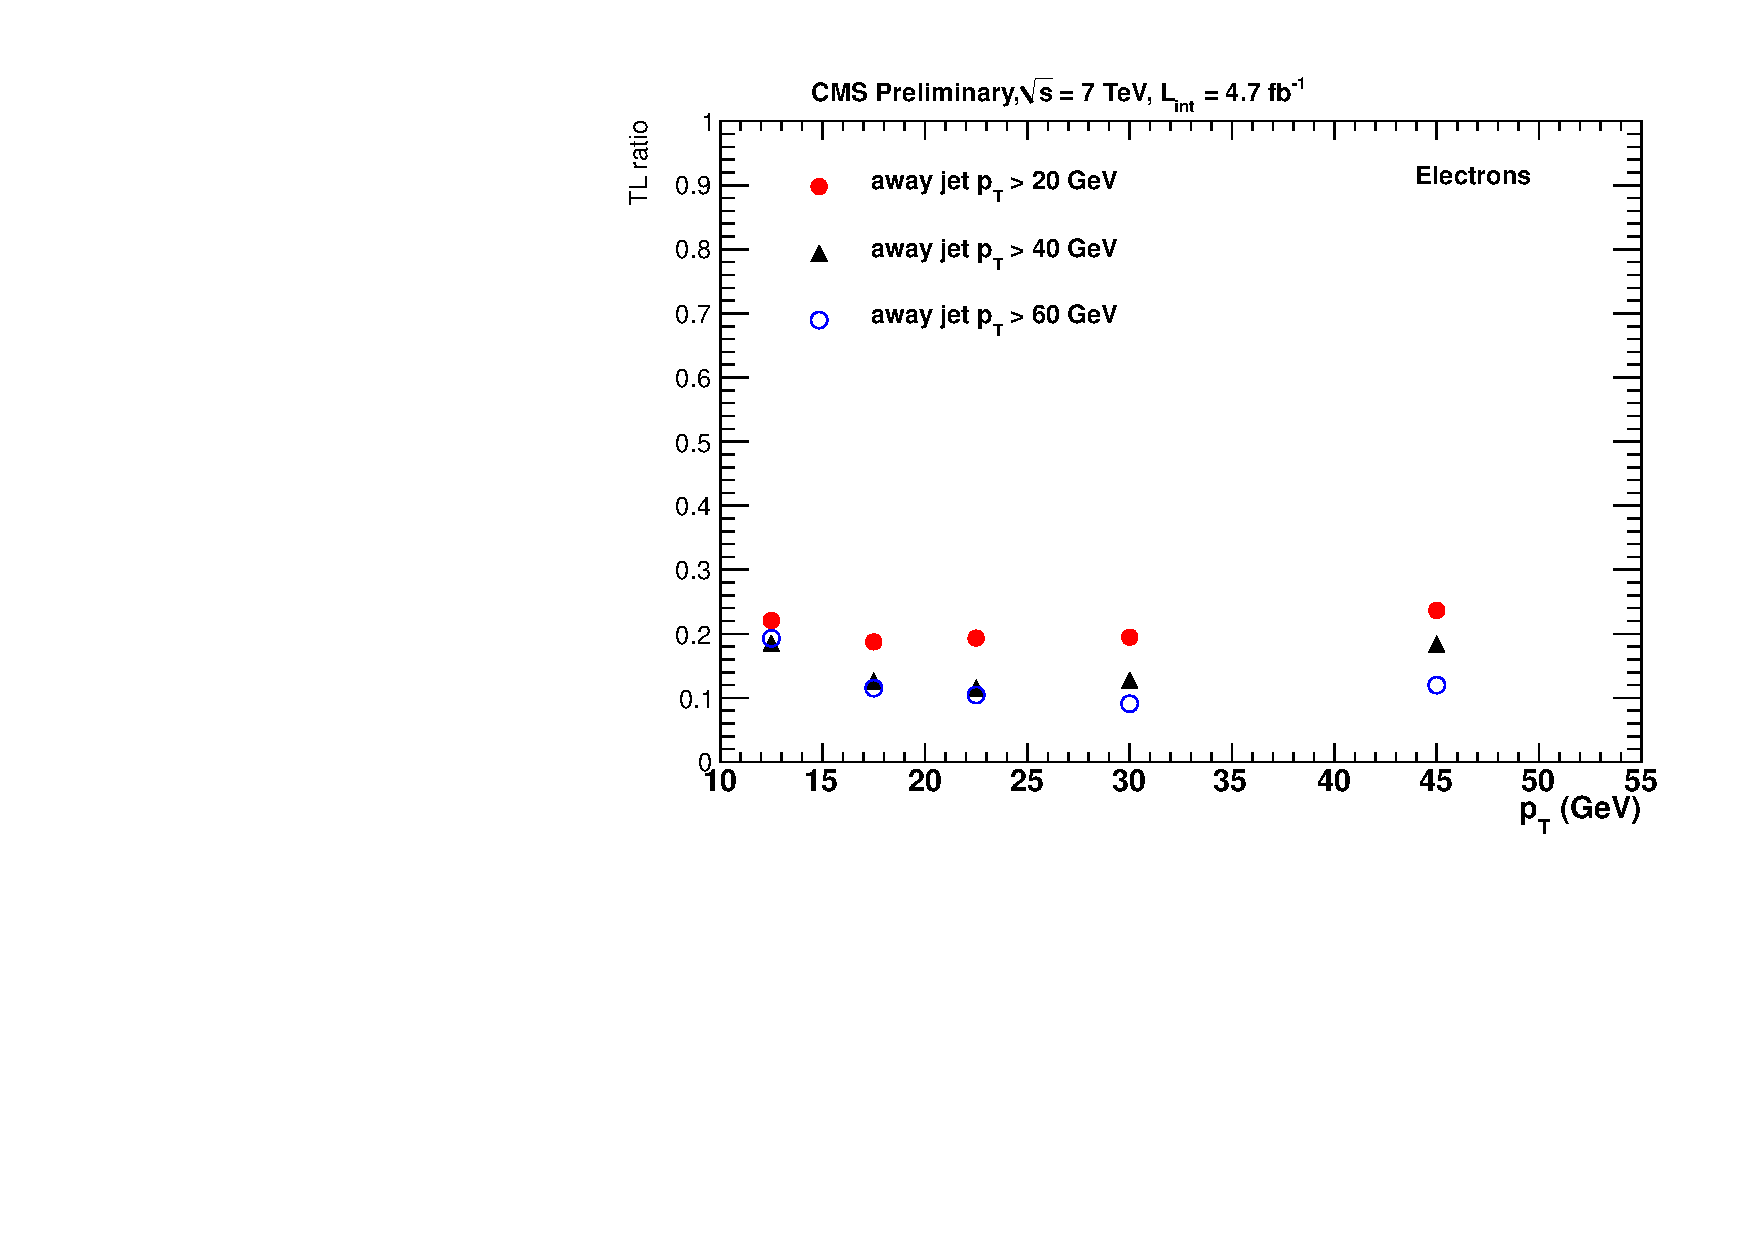
\includegraphics[width=0.48\linewidth]{figs/eleFRcaloIso_data_ptProj}
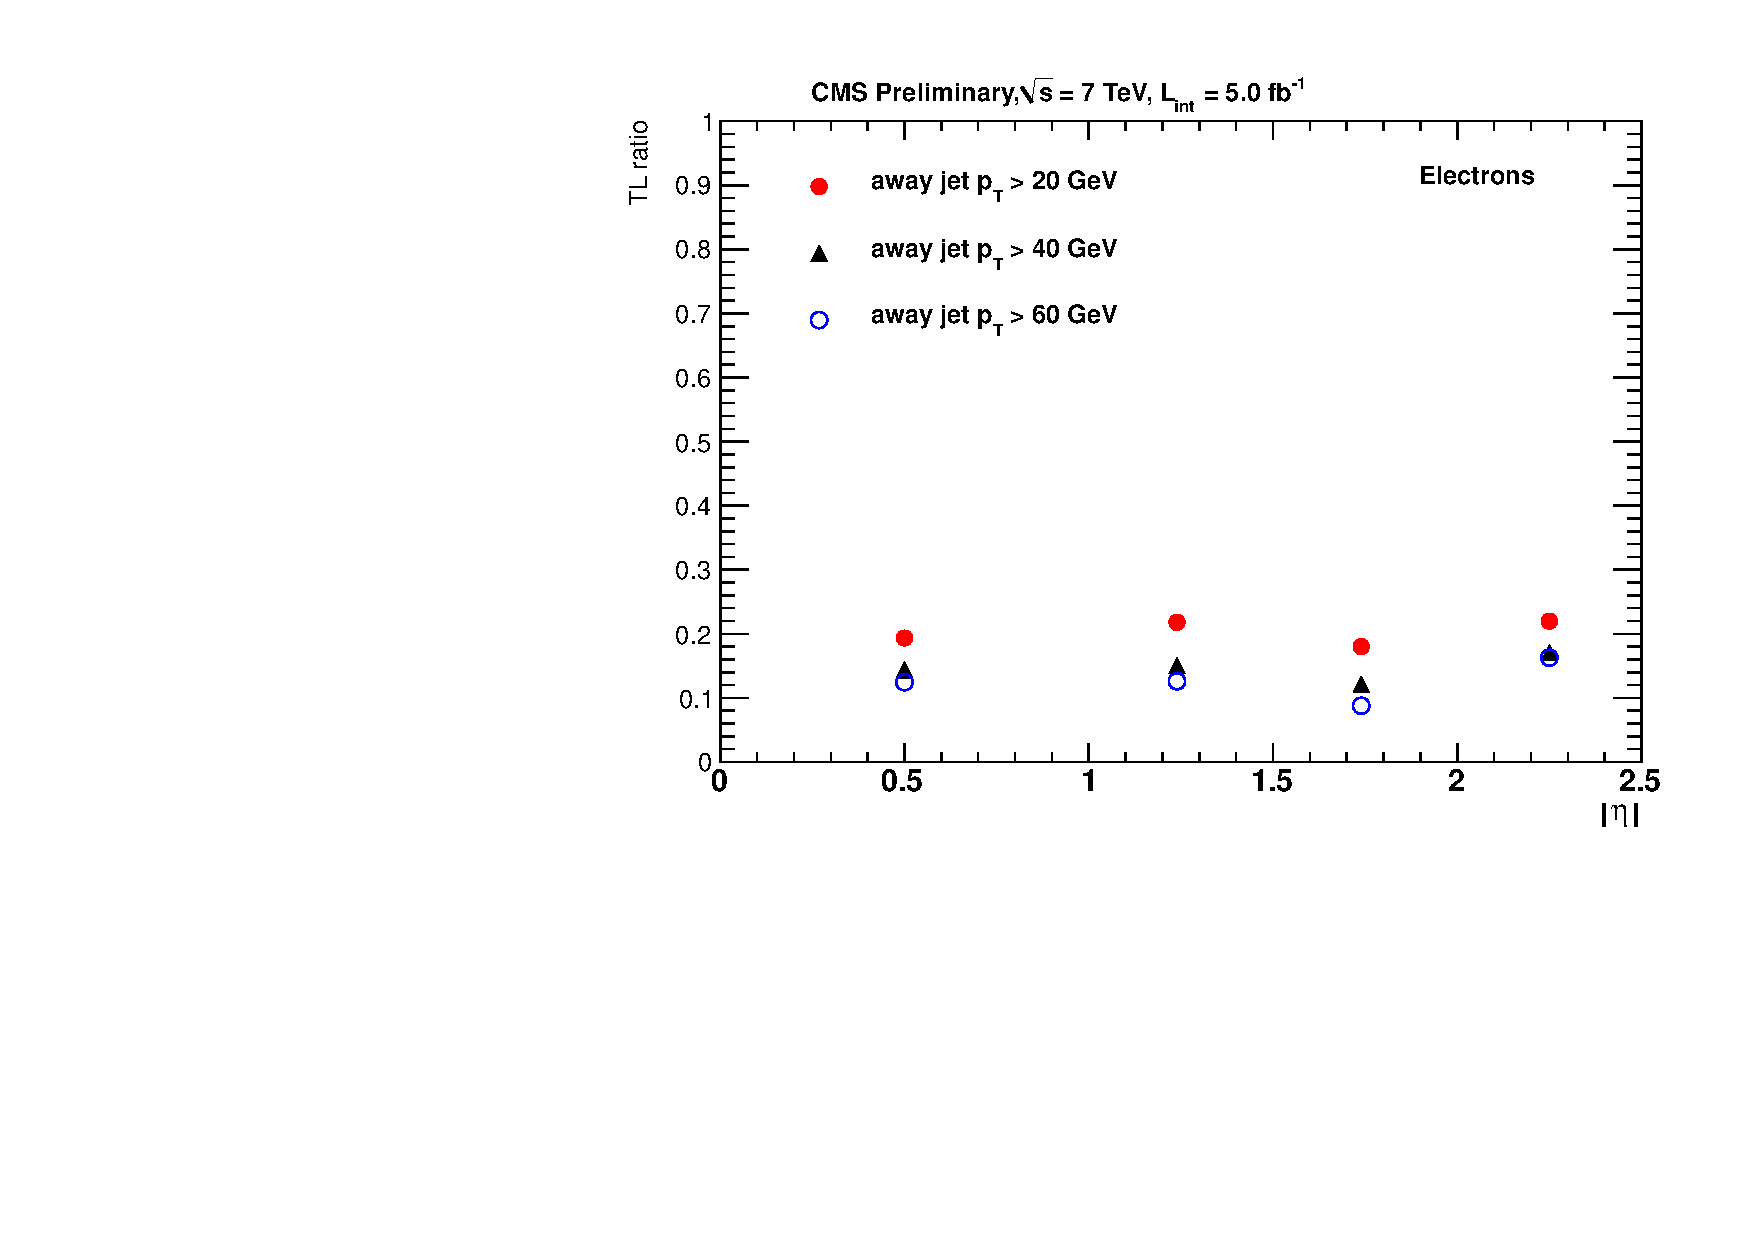
\includegraphics[width=0.48\linewidth]{figs/eleFRcaloIso_data_etaProj}\\
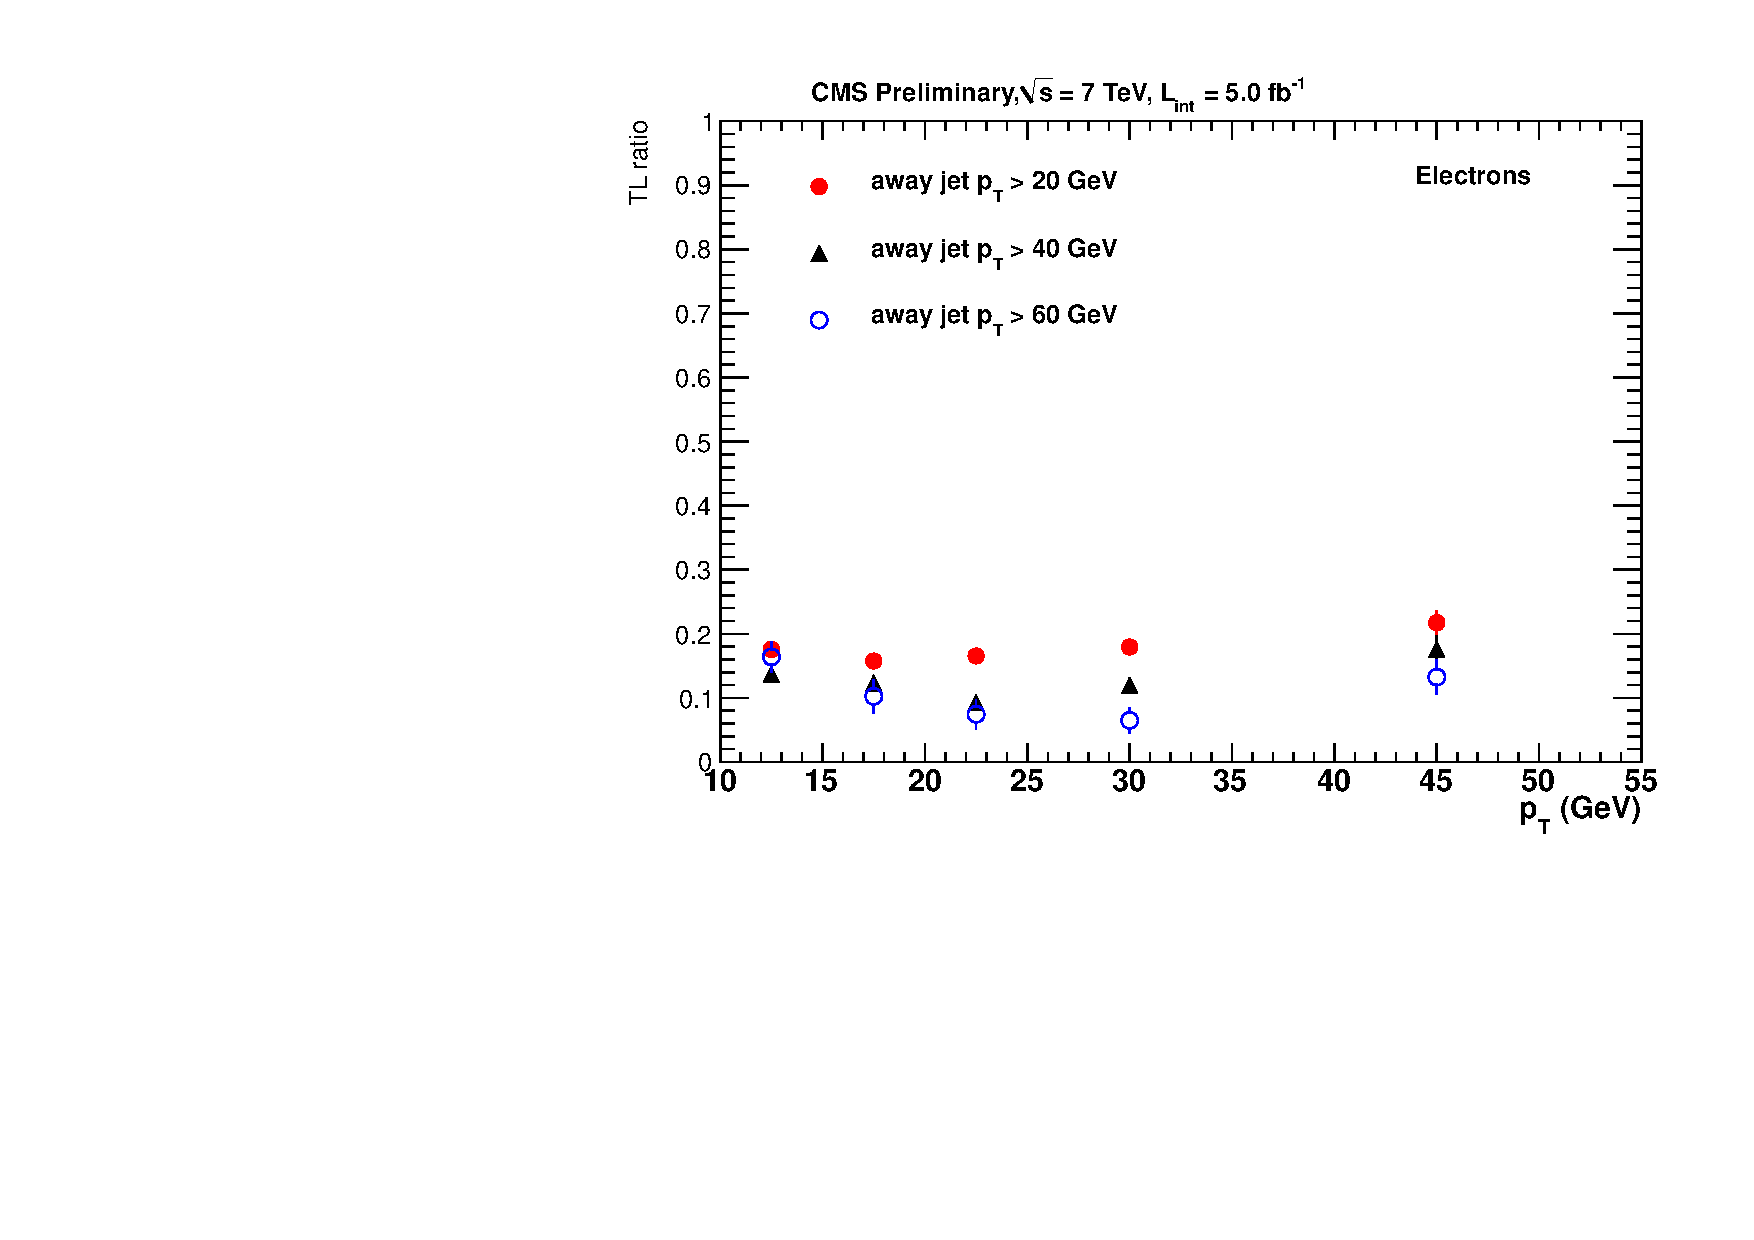
\includegraphics[width=0.48\linewidth]{figs/eleFRnoIso_data_ptProj}
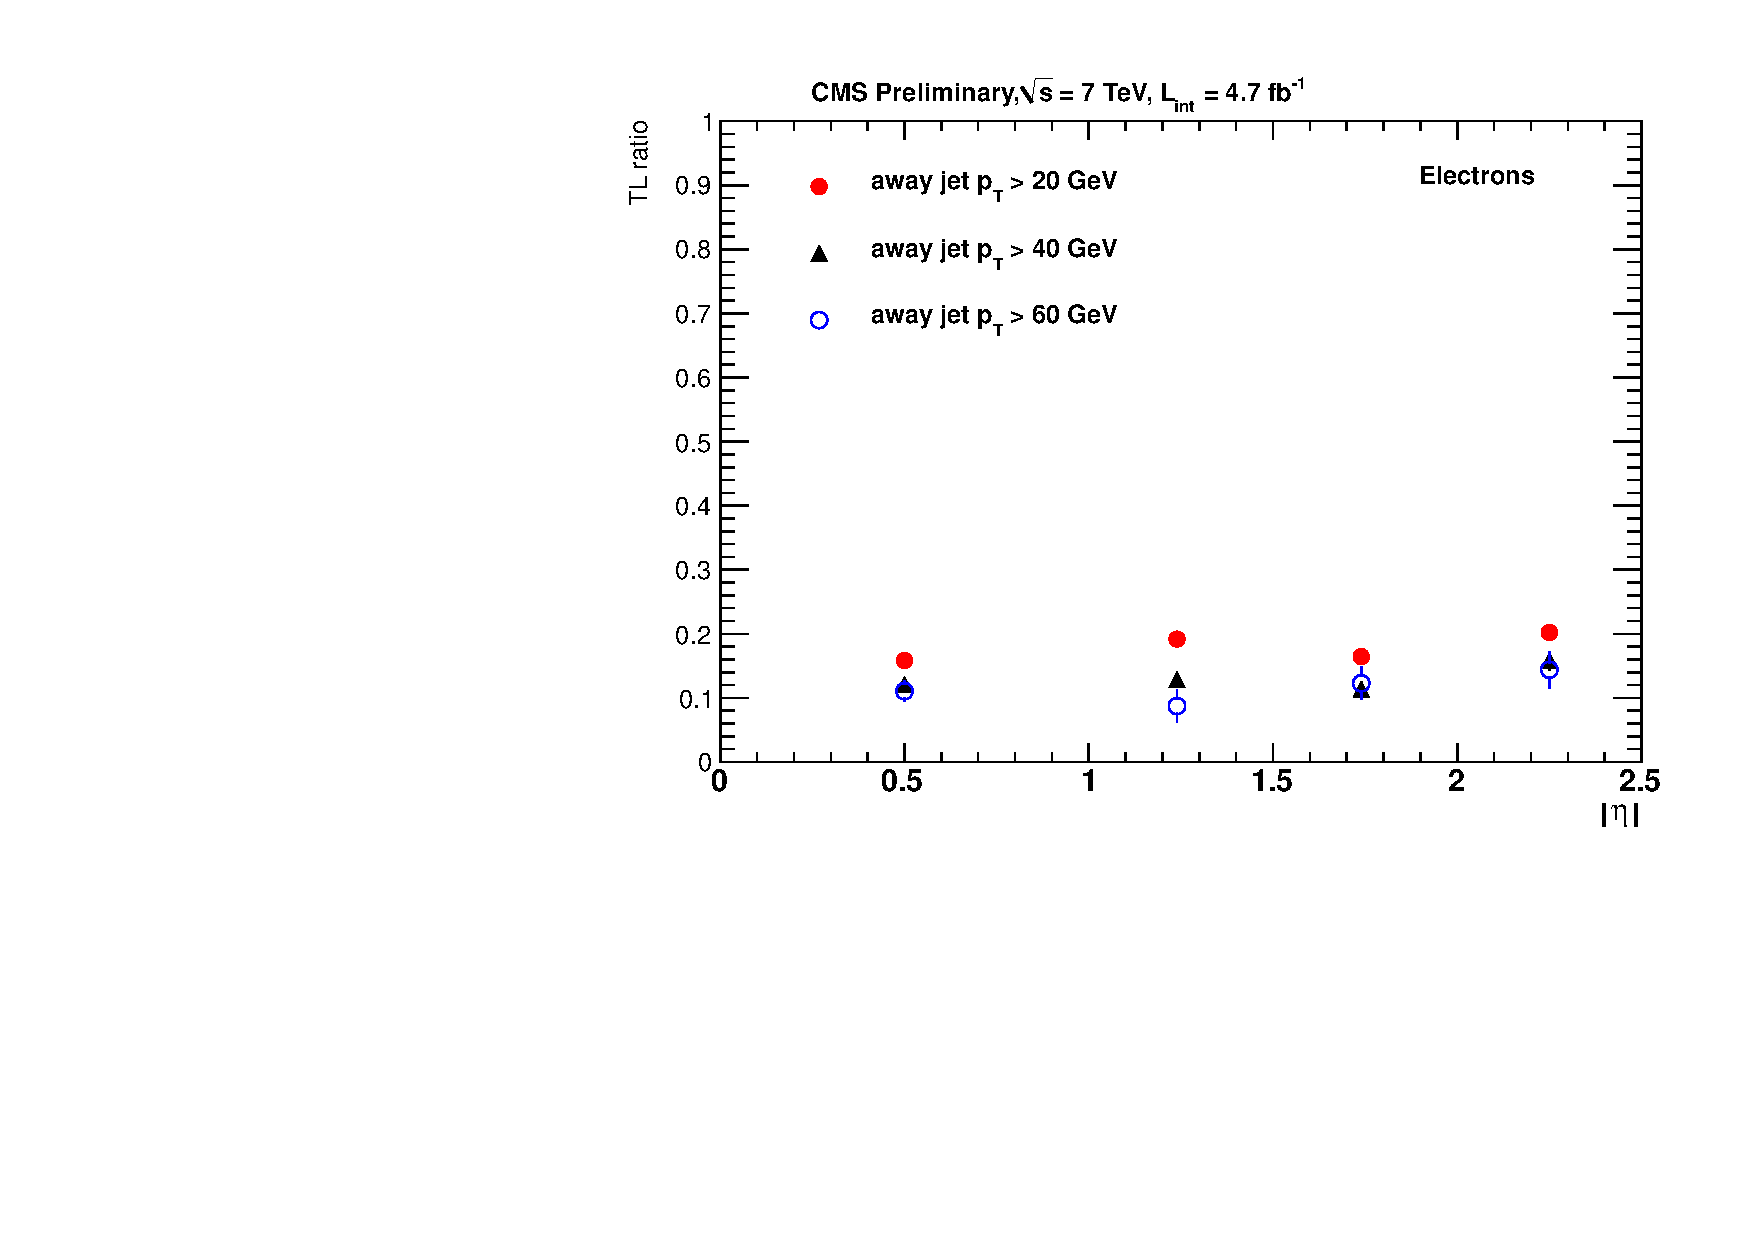
\includegraphics[width=0.48\linewidth]{figs/eleFRnoIso_data_etaProj}
\caption{\label{fig:frelectron}Electron fake rate projected on $\pt$ (left) and $|\eta|$ (right)
for electrons collected by the triggers with calorimeter and tracker isolation requirements (top), with a calorimeter isolation requirement (middle) and without an isolation requirement (bottom).
The fake rates are shown separately for measurements  with a requirement for an away jet \pt\ 
to be above 20~\GeV\ (red filled circles), 40~\GeV\ (black up triangles), and 60~\GeV\ (blue open circles).
}
\end{center}
\end{figure}

\clearpage

%Similar to the choice made in 2010 data analysis, we restrict the measurement of the fake rate
%to 35~\GeV\ (55~\GeV) for muons (electrons) in order to avoid the residual contribution from the W+jets
%and Z events.
%We find that the contribution from the W/Z production is small for electrons up to about 55~\GeV,
%as illustrated in Fig.~\ref{fig:freleptWZ} for data (left) and simulation (right), respectively.
%There is no significant contribution from the W events in the MC, which is supported by only marginal increase
%in the fake rate in data after the W suppression requirements are removed.
%For muons, since the selection did not change significantly, we refer to the corresponding figure 
%in~\cite{frmethod}.
%
%
%\begin{figure}[h]
%\begin{center}
%%\includegraphics[width=0.48\linewidth]{figs/}
%%\includegraphics[width=0.48\linewidth]{figs/}
%\caption{\label{fig:freleptWZ}Electron fake rate as a function of the electron $\pt$ measured
%for a range of selection enhancing the contribution from the W/Z events.
%The fake rate measured in data (left) is shown for the nominal measurement (circles) and for 
%a measurement without additional W suppression (squares) using triggers with a calorimeter isolation requirement.
%The electron fake rate measured in MC (right) is shown for the nominal measurement using 
%only QCD samples (circles), and that with the W sample included (up triangles),
%as well as for the selection without the W suppression measured in the QCD sample alone (squares)
%and that with the W sample included (down triangles).
%}
%\end{center}
%\end{figure}
%
%The following assumptions are made prior to applying the measured fake rates to the dilepton events.
%\begin{itemize}
%\item The fake rate per lepton is independent for the two leptons, e.g. 
%	to predict the fake contribution to an $e\mu$ final state we consider electron and muon fakes
%          separately, and add them up, assuming no correlations between the two estimates.
%\item We assume the lepton fake rate measurement in an inclusive QCD sample as 
%	described in~\cite{frmethod} represents the lepton fake rate  in the dilepton sample. 
%\end{itemize}

We test that the fake rates measured in QCD are applicable to the dilepton samples by performing closure
tests on simulated W+jets, \ttbar, and QCD samples.
The tests done on W+jets and \ttbar\ samples are done as follows
\begin{enumerate}
\item select events passing the baseline selections;
\item require that one lepton is matched to a leptonic W decay and the other (fake) lepton is not
matched to a leptonic W decay;
\item scale the number of fake leptons failing the full lepton selections and passing the FO selections
	by $FR/(1-FR)$ as a function of the fake lepton \pt\ and $|\eta|$ --- this is the prediction
	of the number of fakes passing full lepton selections;
\item compare the predicted and observed number of fake leptons.
\end{enumerate}
The prediction of the number of events with fakes gives a consistent overestimate for the \ttbar\ events
for both electrons and muons by approximately the same fraction of  $70\%$ of the observed value,
or, equivalently, the observed value differs from the prediction by approximately  40\% of the predicted value.
We attribute this to the difference in the underlying parton momenta in \ttbar\ and inclusive QCD events:
the momentum is generally higher in \ttbar\ events, which corresponds to a smaller effective fake rate.
We find that the prediction of the number of fakes gives a marginally significant underestimate 
for W+jets events.
The statistical uncertainty of this test  is much larger for muons than for electrons.
We expect this to happen if the jets initiating the fakes in W+jet events have a smaller momentum on average
compared to those used to extract the fake rate in QCD events.
Results of the closure tests on \ttbar\ and W+jet events passing the baseline selections of {\em high-\pt}
 dileptons are summarized in Table~\ref{tab:ttWjclosure}.
In addition to this, we have performed a closure test on the same-sign dimuon events in the QCD sample
(without any additional requirement on the number of jets or on \met):
we find that the number of expected events agrees with the  observed within statistical uncertainty of about 20\%.

\begin{table}[h]
\begin{center}
\begin{tabular}{lc|cc|cc}
\hline\hline
Sample	& result	&	\multicolumn{2}{|c}{ElectronFR}		& \multicolumn{2}{|c}{Muon FR}	\\
	&		&	$ee$		& $e\mu$		& $\mu\mu$	& $e\mu$	\\\hline
\ttbar	&	observed& $2.8\pm0.2$		& $4.2\pm0.2$		& $3.9\pm0.2$	& $4.0\pm0.2$	\\
	&predicted	& $4.9\pm0.4$		& $6.8\pm0.5$		& $7.2\pm 0.3$	& $6.5\pm 0.2$	\\ 
	&	ratio	& $1.8\pm0.2$		& $1.6\pm0.2$		& $1.8\pm 0.1$	& $1.6\pm 0.1$	\\ \hline
W+jets	&	observed& $<2.1$		& $8.4\pm4.2$		& \multicolumn{2}{|c}{$2.1\pm 2.1$} \\
	&  predicted	& $1.5\pm0.8$		& $3.4\pm1.4$		& \multicolumn{2}{|c}{$2.1\pm1.2$}	\\
	& ratio		& $<1.4$		& $0.4\pm0.3$		& \multicolumn{2}{|c}{$1.0\pm1.2$} \\
\hline\hline
\end{tabular}
\caption{\label{tab:ttWjclosure}Fake rate closure test on \ttbar\ and W+jets events for high-\pt\ dilepton
selections. 
The muon FR test in $e\mu$ is done with $\met>20~\GeV$.
The number of events is scaled to 1~\fbin.
Expcept for the test in \ttbar\ with electrons (done with jet $\pt>40~\GeV$), 
the results are reported for events with at least two jets with $\pt>30~\GeV$ (old selection), used to 
increase the number of events passing the selections.}
\end{center}
\end{table}

\newcommand{\nNoNu}{\ensuremath{N_{{n}\overline{n}}}}
\newcommand{\nNoNo}{\ensuremath{N_{\overline{n}\overline{n}}}}
\newcommand{\nNuNu}{\ensuremath{N_{{n}{n}}}}

%An estimate of the number of fake leptons in dilepton events passing full (numerator) selections
%is based on counts of dilepton events with two non-numerator \nNoNo, two numerator \nNuNu,
%and only one non-numerator object \nNoNu.
%Assuming \nNoNo\ is dominated by QCD (both leptons are fake), a relatively simple calculation
%leads to the following, neglecting much smaller terms.
%The QCD contribution to the signal sample $N^{QCD}_{nn}$ is given by
%$$
%N^{QCD}_{nn} = \sum_{i,j} \frac{FR_i FR_j}{(1-FR_i)(1-FR_j)} \nNoNo^{ij},
%$$
%where the indices $i, j$ correspond to the binning and flavor of corresponding non-numerator lepton objects.
%The contribution from one true and one fake lepton (e.g. $t\bar{t}$, single top, Wjets) 
%contribution in the signal sample $N^{W}_{nn}$ is given by
%$$
% N^{W,raw}_{nn} = \sum_{i} \frac{FR_i}{(1-FR_i)} \nNoNu^{i},
%$$
%$$
% N^{W}_{nn} =  N^{W,raw}_{nn} -  2 N^{QCD}_{nn}.
%$$
%
%The total prediction of the number of events with fake leptons is thus
%$$
% N^{fakes}_{nn} =  N^{W}_{nn} +  N^{QCD}_{nn}. 
%$$
The systematic uncertainty of $\pm 50\%$ per fake lepton is estimated for the fake rate method.
It is justified based on the closure tests and an understanding that the variation of the fake rate on
the jet momentum corresponds to the variation between the fakes from the ISR/FSR jets (like in W+jets),
and jets from the heavy final states (as in \ttbar).
We compute the contributions from QCD and W+jets and assign a 50\% systematic
uncertainty on the combined estimate.

We have neglected any "signal contamination". 
Signal contamination enters when there is a significant
source of two isolated leptons, with one or both failing the numerator cuts, but passing the denominator cuts
comprising  a significant fraction of the total number of \nNoNu\ or \nNoNo\ samples. 
Without an additional correction that can be easily applied,
a contribution from events with two real same-sign dileptons failing the numerator selections
 will overestimate the background contribution by approximately 3\% of the count of
the real same-sign dileptons passing the numerator selections.
Considering the size of the uncertainty on the background,
this effect can be safely ignored in the estimates 
of the fake leptons until the rate of same-sign dileptons passing the full
selections is at least an order of magnitude  higher than that expected
from fakes alone.
%As we see no evidence of any signal excess, we can safely ignore this.

%%%%%%%%%%
%%%%%%%%%%
%%%%%%%%%%
%%%%%%%%%%
%%%%%%%%%%
%%%%%%%%%%
%%%%%%%%%%
%%%%%%%%%%

\subsection{Data Driven prediction for charge mis-reconstruction backgrounds}
\label{sec:flips}

%%%%%%%%%%
%%%%%%%%%%

Following our original studies~\cite{sspaper2010} of the electron charge misreconstruction, 
we apply the requirement for electrons that all three charge measurements for a GSF electron agree. 
This dramatically reduces the rate of charge mismeasurement for electrons to the point where it 
is an almost negligible source of background, less than 10\% of the background due to fake leptons, 
as was shown in the 2010 analysis~\cite{sspaper2010}.
Even though this background is small, it is not necessarily well-reproduced in simulation.
We apply a data-driven method used in the previous analysis here.

The following steps are done:
\begin{enumerate}
\item Measure the probability for an electron to have its charge misreconstructed 
in bins of $|\eta |$ and $\pt$ using single electron gun Monte Carlo.
\item Use this probability and apply it to the opposite sign Z sample for a Z control sample 
defined as $76$\ GeV $ < m_{ll} < 106$\ GeV,  \met $ < 20$\ GeV,
and transverse mass $< 25$ GeV. 
Here transverse mass is calculated based on whichever lepton has higher $\pt$. 
Compare with the actual yield of double-charged Z candidates in that region to establish validity of the approach.
\item If the expected and observed yields agree reasonably well in the previous step, continue using
	the probability measured in the first step and use the discrepancy as a systematic uncertainty.
\item Then apply this probability to all the electrons in opposite sign dilepton events that pass the selection. 
	This produces the data driven charge flip  prediction shown in the tables in Section~\ref{sec:yields}. 
\item The lepton $p_T$ distributions of leptons from top is slightly harder than that for leptons from Z. The above
test thus does not fully sample the lepton spectrum for our background sample. We assign an additional systematics
to account for this effect.
\end{enumerate}

Figure~\ref{fig:flipvsptOrEta} shows the $\pt$ (left) and $|\eta |$ (right) projections of 
the charge mismeasurement probability  from single electron gun Monte Carlo.
The same function is applied to data and MC.  
As seen in Fig.~\ref{fig:flipvsptOrEta} (right), the charge mismeasurement probability
did not change substantially in the samples used for the previous analysis, as well as for the Spring11 and Summer11
simulation.

\begin{figure}[h]
\begin{center}
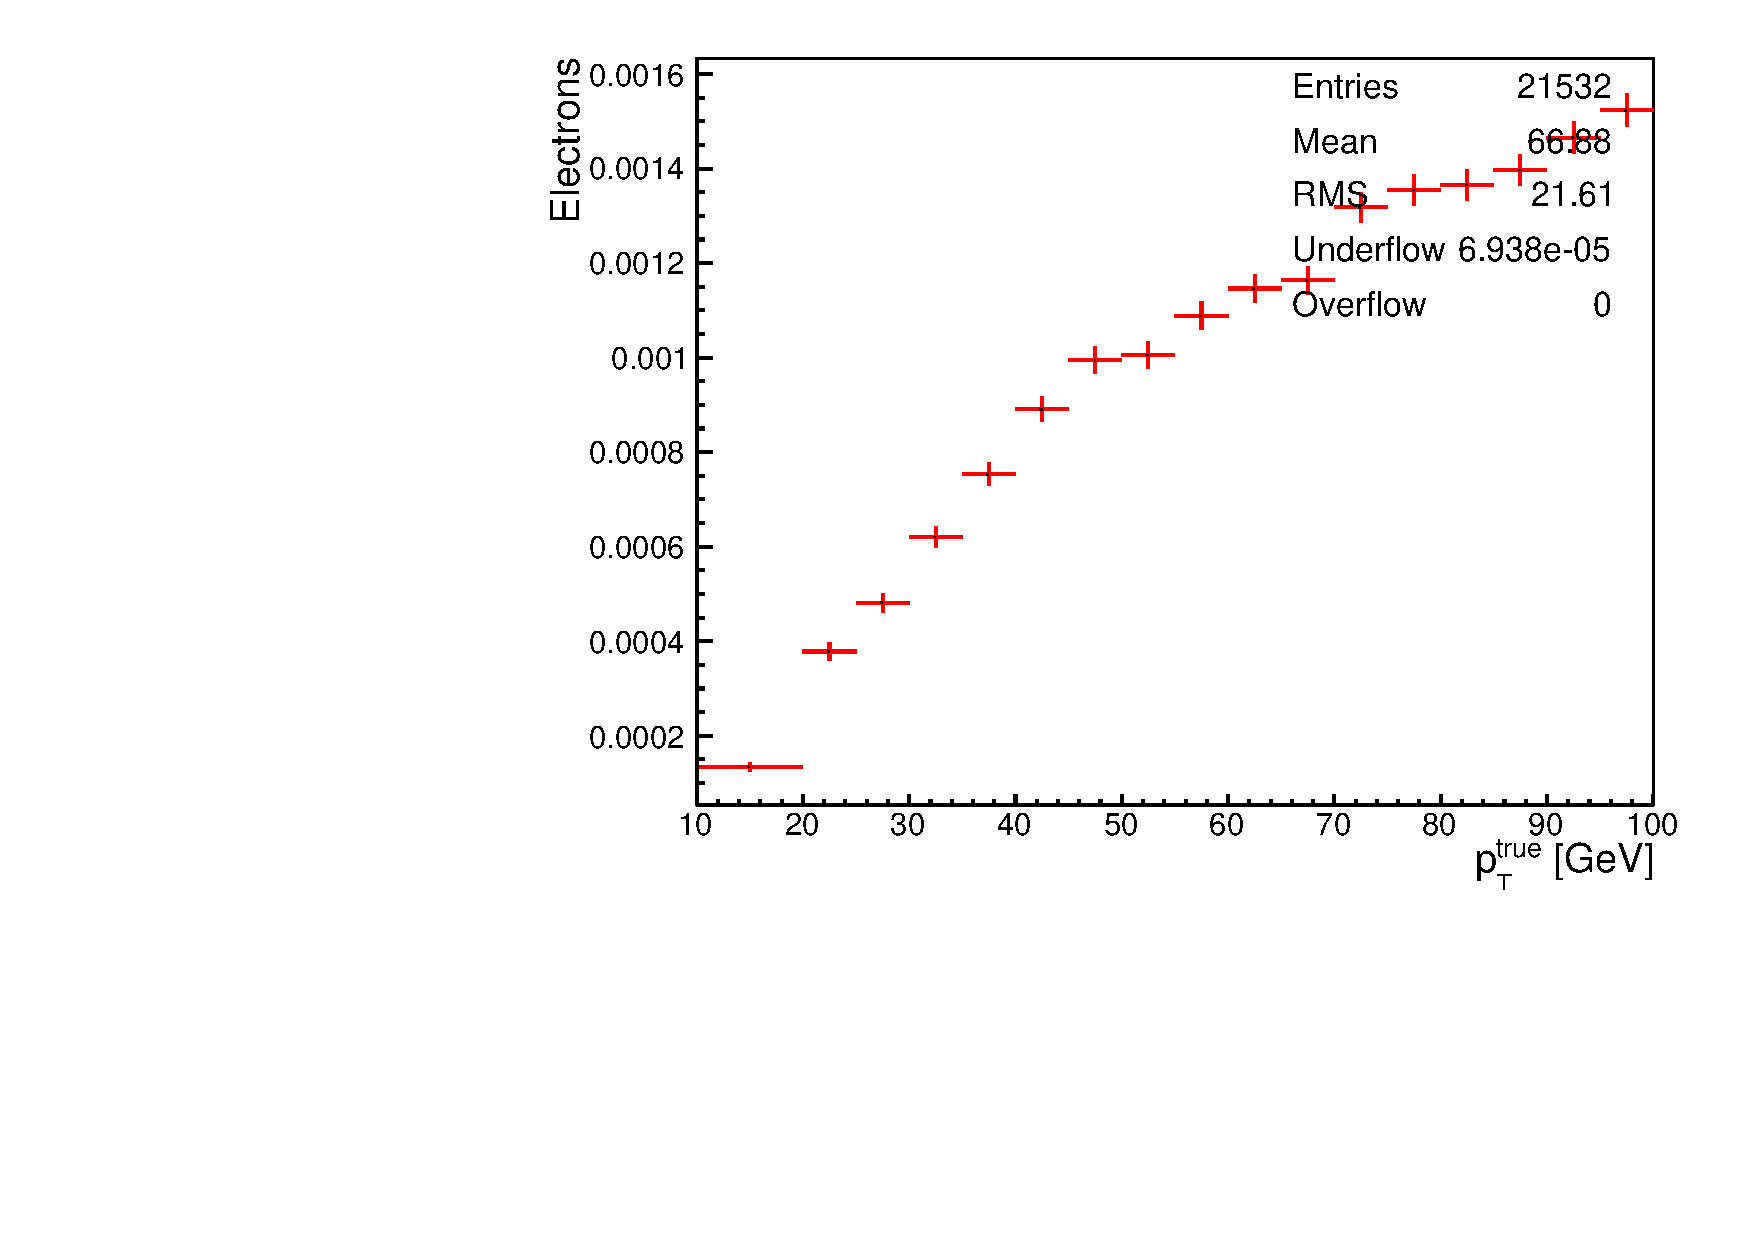
\includegraphics[width=0.47\linewidth]{figs/flipRate2011VsPt}
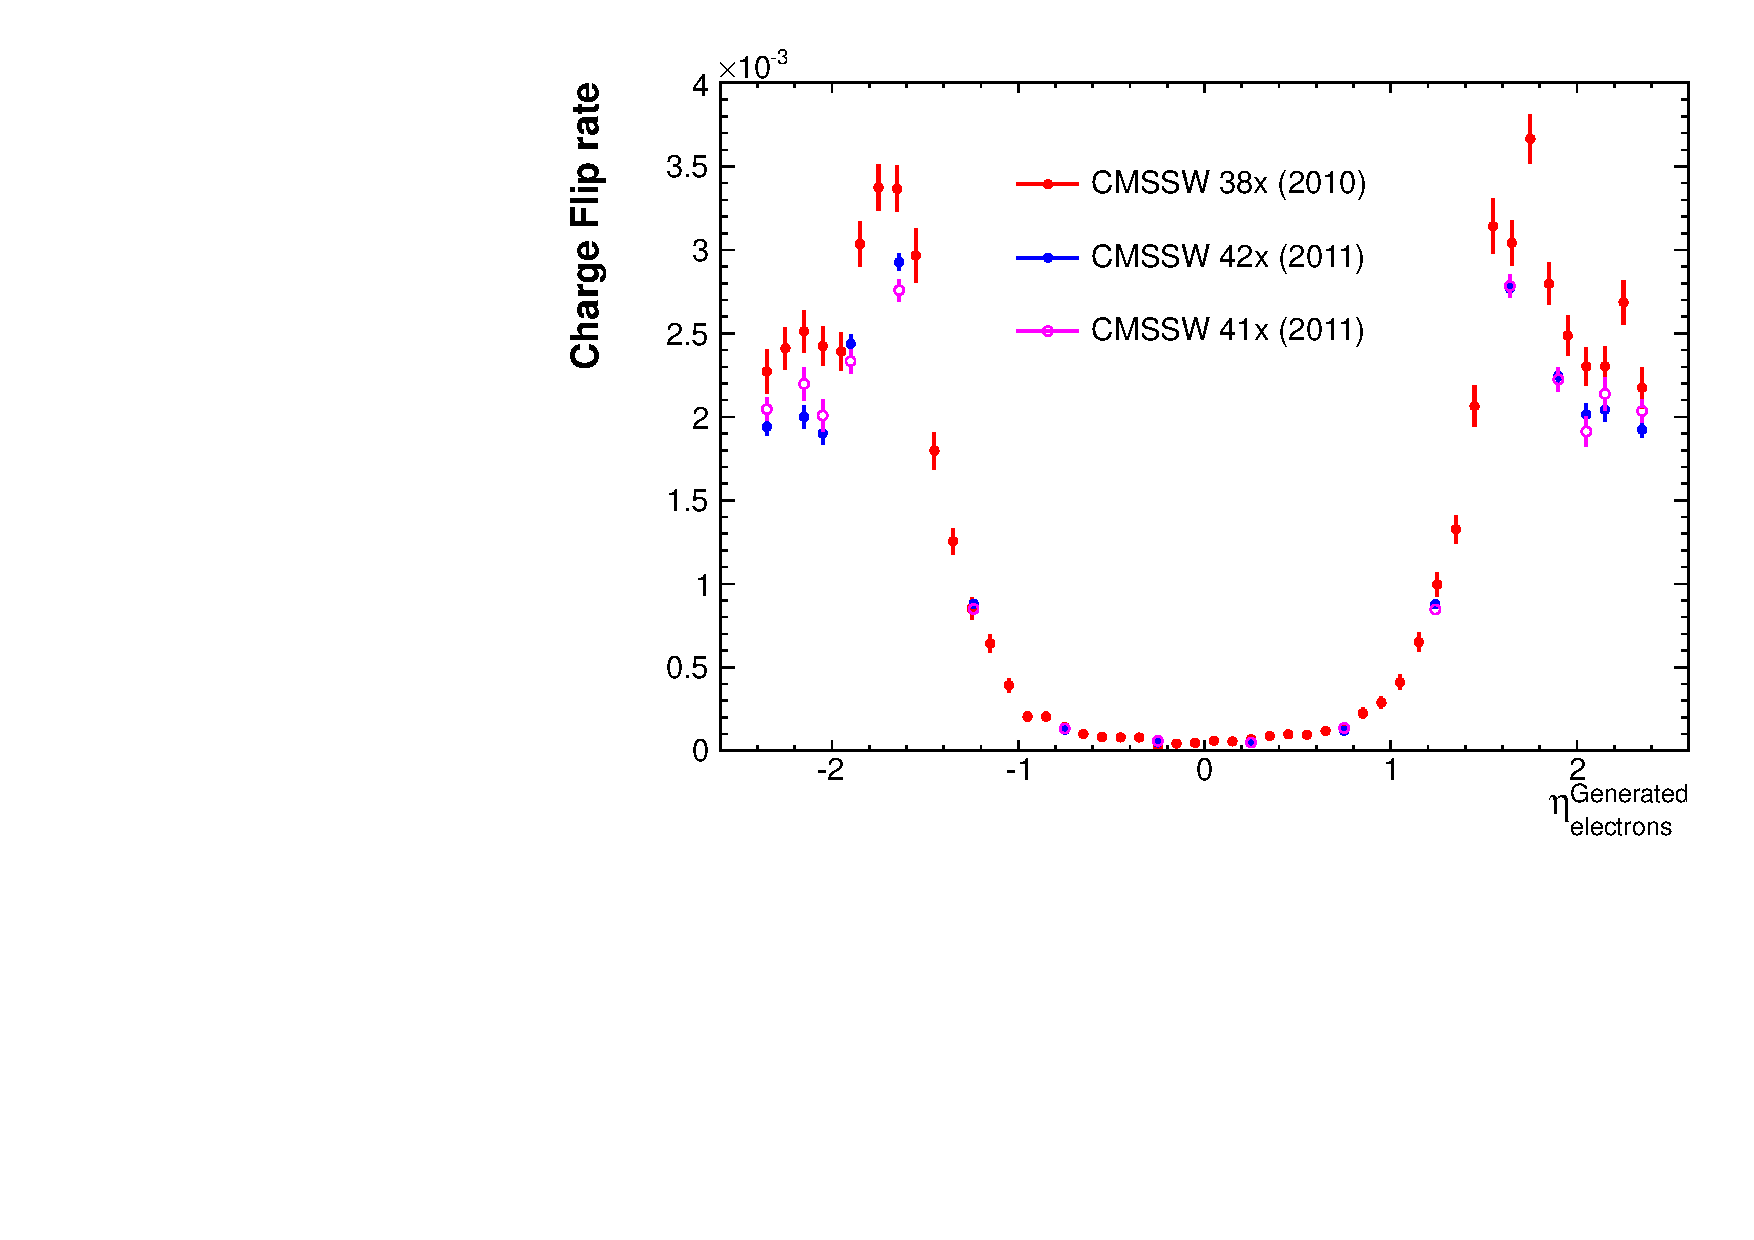
\includegraphics[width=0.47\linewidth]{figs/flipRate2011PAS}
\caption{\label{fig:flipvsptOrEta}Charge mismeasurement probability from single electron gun MC
shown in projections on $\pt$ (left) and $\eta$ (right).
The projection on $\eta$ also shows the distributions for the charge mismeasurement probability
in 2010 analysis (red), current definition (blue), and that in the older (Spring11-like) MC sample.}
\end{center}
\end{figure}

We find 390 events with same-sign electron pairs in data in the Z control region.
This needs to be compared with the sum of the expected same-sign events as estimated from
opposite-sign dielectrons, $359.7\pm4.1$, plus a contribution from fakes, $11\pm 6$.
The number of events expected directly from simulation is  $469\pm 11$.
The same-sign dielectron mass distribution observed in data is compared to the expectation from
simulation in Fig.~\ref{fig:flipZee}.
These comparisons are consistent within statistics.
The uncertainty is taken to be 20\% to account for kinematic differences between leptons from Drell-Yan events and top pairs, the latter expected to be the dominant source of background events for this analysis.
%Based on these observations we assign a correction factor of $1.2\pm0.2$ to 
%the expected number of same-sign dielectron
%events obtained using the opposite-sign dielectron samples.
%The scale factor corresponds to the relative difference between $121\pm11({\rm stat.})\pm 4({\rm syst})$ 
%and $100\pm 0.3$, the uncertainty is taken to be 20\% to account in addition for potential effects
%not covered by this test with Z events.


\begin{figure}[h]
\begin{center}
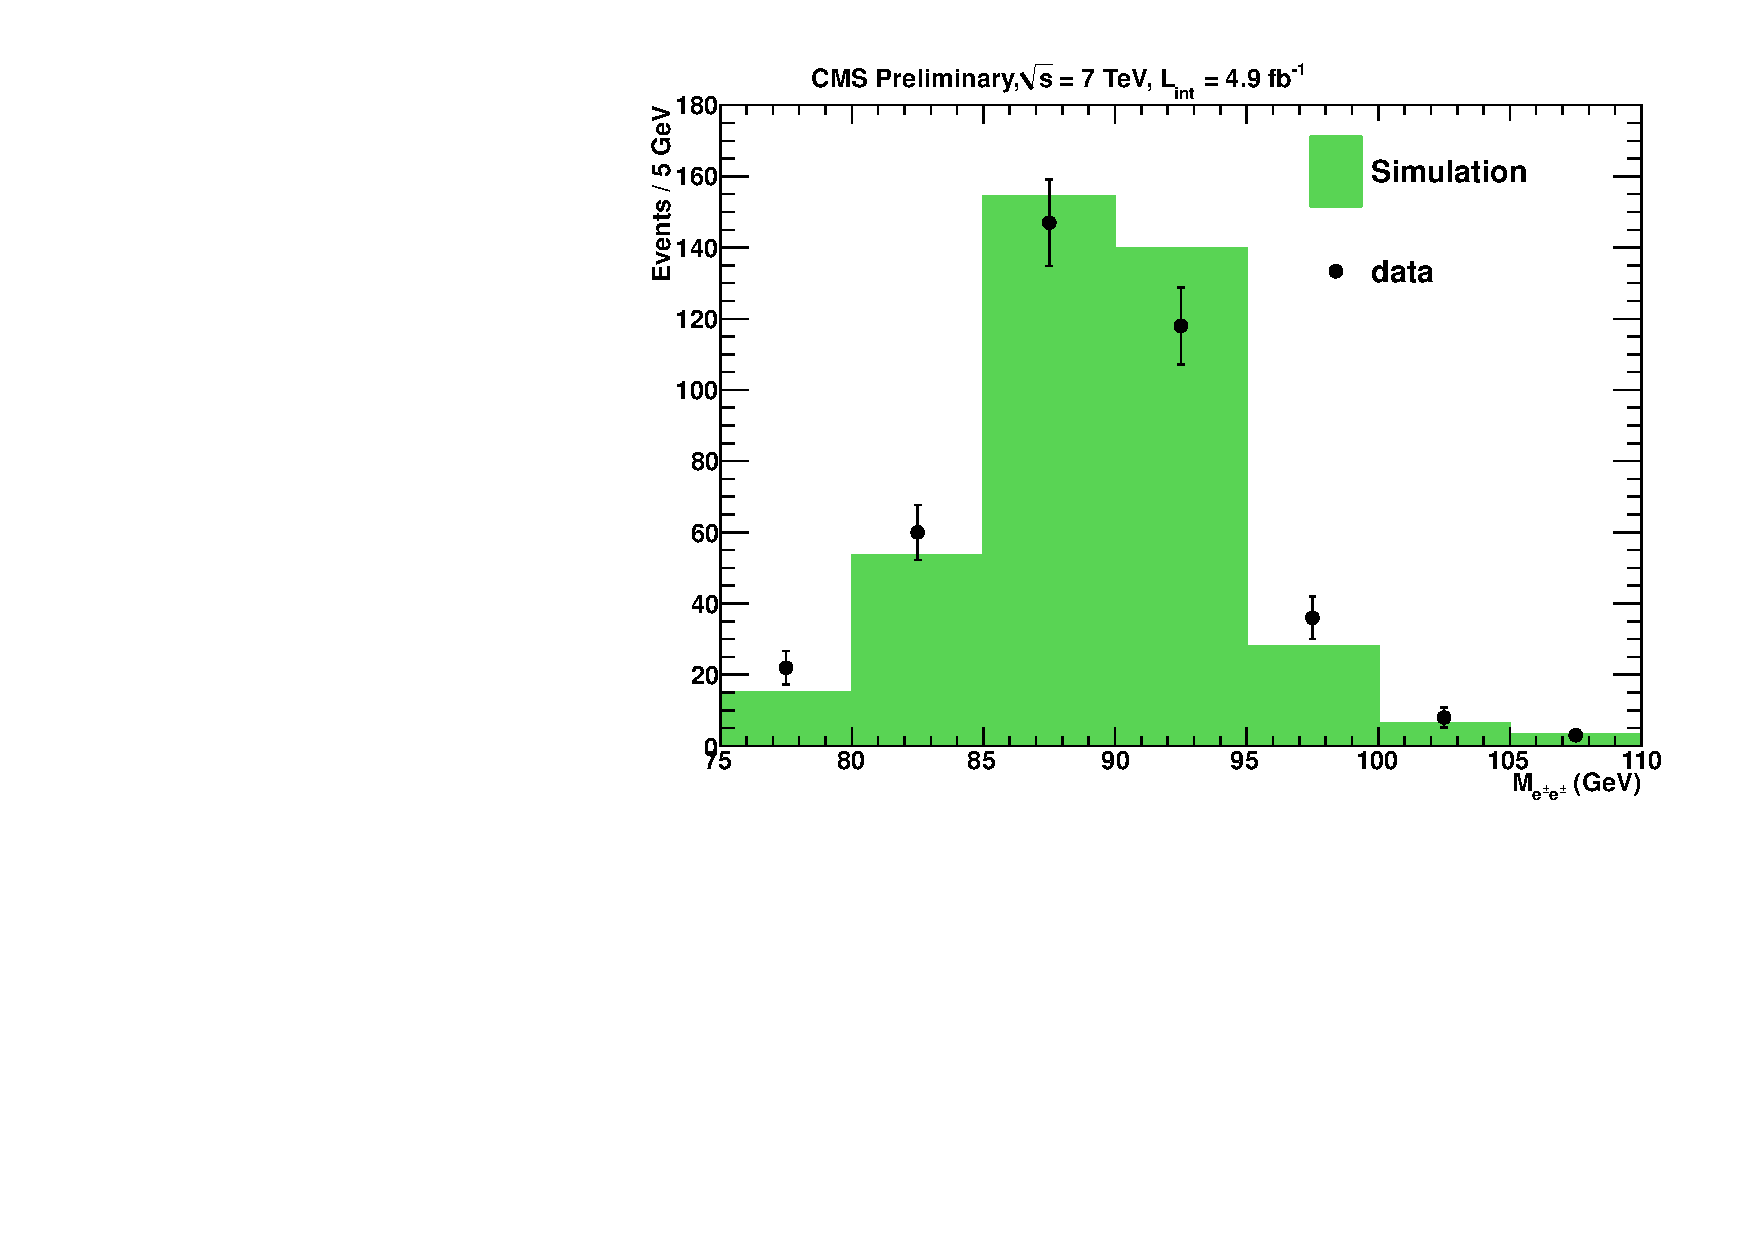
\includegraphics[width=0.8\linewidth]{figs/qflip_data_mc_comp}
\caption{\label{fig:flipZee}
Same sign $ee$ invariant mass distribution compared with $Z \to ee$ Monte Carlo expectations.
Cuts on missing transverse energy $<$ 20 GeV and transverse mass
$<$ 25 GeV have been applied to reduce backgrounds from $W +$ jets.
The highest $\pt$ lepton has been used in the calculation of the transverse  mass.}
\end{center}
\end{figure}










\section{Event Yields and Background Estimation}
\label{sec:yields}

In the following Tables~\ref{tab:yield_baselinenomet} 
to~\ref{tab:yield_ht320nomet}
we summarize the background 
estimates and compare them to the
observed counts of events in data for the baseline and search region selections
defined in Sections~\ref{sec:eventsel} and~\ref{sec:regions}.
In each table the expectations from the simulation alone are given 
in the upper part.
 These are used to get a feeling of the expected contributions.
Among these MC expectations, 
only those with actual final state 
isolated same-sign leptons are used for the final result
as described in Section~\ref{sec:bkgds}.
The lower part of each table is the main result of the analysis
used for comparisons with data and setting constraints on various models.
These include the predictions for the fake-lepton and charge misidentification
backgrounds derived as described in Section~\ref{sec:datadriven}.

To reiterate and make it absolutely clear.  The total background
prediction in a given signal region
is the sum of three distinct components:
\begin{enumerate}

\item The data-driven charge misidentification prediction (row ``Charge Flips'' in
Tables~\ref{tab:yield_baseline} to~\ref{tab:yield_ht320met120}).

\item The data-driven sum of single fakes (SF) and double fakes
(DF) predictions (row ``SF$+$DF''
in Tables~\ref{tab:yield_baseline} to~\ref{tab:yield_ht320met120}).

\item The total MC prediction for processes that naturally give isolated
same-sign dileptons, see Section~\ref{sec:bkgds} (row ``MC Pred'' in
Tables~\ref{tab:yield_baseline} to~\ref{tab:yield_ht320met120};
this is the sum of the rows starting from ``$V\gamma$'' down to 
and including the tribosons -- although in practice only $ttW$ and 
$ttZ$ matter).  Note that for the dominant physics 
backgrounds we normalized the MC to $\sigma(pp \to ttW) = 0.1633 \pm 0.082$
pb and $\sigma(pp \to ttZ) = 0.139 \pm 0.070$ pb.

\end{enumerate}

Details on the systematics of the background predictions are given in the corresponding sections.
The final estimates on these uncertainties are rather simple:
\begin{enumerate}
\item The charge flip contribution has a 20\% systematic.
  \item The predicted number of fakes has a 50\% systematic in all modes.
  \item The MC prediction for ``real'' same-sign isolated dileptons
    has an uncertainty of 50\%.
  
\end{enumerate}

\newcommand{\ttdilS}{\ensuremath{\ttbar\to\ell\ell X}}
\newcommand{\ttslbS}{\ensuremath{\ttbar\to\ell(b\to\ell) X}}
\newcommand{\ttsloS}{\ensuremath{\ttbar\to\ell(b\!\!\!/\to\ell) X}}
\newcommand{\SFnn}{\ensuremath{N^{\rm Wj,raw}_{nn}}}

\begin{table}[h]
\begin{center}
\begin{tabular}{l | l l l l}
\hline\hline
 Source  &  ee  &  $\mu\mu$  &  e$\mu$  &  all \\
\hline
$t\overline{t}\rightarrow \ell\ell X$ &  0.751 $\pm$  0.118 &  0.000 $\pm$  0.014 &  0.840 $\pm$  0.124 &  1.591 $\pm$  0.171\\
$t\overline{t}$ other &  0.013 $\pm$  0.013 &  0.000 $\pm$  0.014 &  0.000 $\pm$  0.014 &  0.013 $\pm$  0.013\\
$t\overline{t}\rightarrow \ell(b\rightarrow \ell)X$ &  0.093 $\pm$  0.042 &  0.153 $\pm$  0.052 &  0.214 $\pm$  0.067 &  0.460 $\pm$  0.095\\
$t\overline{t}\rightarrow \ell(\slashed{b}\rightarrow \ell)X$ &  0.713 $\pm$  0.116 &  0.040 $\pm$  0.026 &  0.836 $\pm$  0.129 &  1.589 $\pm$  0.175\\
\hline
$t$, s-channel &  0.000 $\pm$  0.061 &  0.000 $\pm$  0.061 &  0.000 $\pm$  0.061 &  0.000 $\pm$  0.061\\
$t$, t-channel &  0.121 $\pm$  0.091 &  0.000 $\pm$  0.058 &  0.000 $\pm$  0.058 &  0.121 $\pm$  0.091\\
$tW$ &  0.000 $\pm$  0.048 &  0.000 $\pm$  0.048 &  0.085 $\pm$  0.070 &  0.085 $\pm$  0.070\\
\hline
$Z\rightarrow ee$ &  0.000 $\pm$  0.457 &  0.000 $\pm$  0.457 &  0.000 $\pm$  0.457 &  0.000 $\pm$  0.457\\
$Z\rightarrow\mu\mu$ &  0.000 $\pm$  0.457 &  0.000 $\pm$  0.457 &  0.000 $\pm$  0.457 &  0.000 $\pm$  0.457\\
$Z\rightarrow\tau\tau$ &  0.000 $\pm$  0.457 &  0.000 $\pm$  0.457 &  0.000 $\pm$  0.457 &  0.000 $\pm$  0.457\\
$W$+jets &  0.000 $\pm$  1.924 &  0.000 $\pm$  1.924 &  0.000 $\pm$  1.924 &  0.000 $\pm$  1.924\\
$WW$ &  0.000 $\pm$  0.020 &  0.000 $\pm$  0.020 &  0.000 $\pm$  0.020 &  0.000 $\pm$  0.020\\
\hline
V$\gamma$ &  0.000 $\pm$  0.264 &  0.000 $\pm$  0.264 &  0.000 $\pm$  0.264 &  0.000 $\pm$  0.264\\
$W\gamma^{*}\rightarrow\ell\nu e e$ &  0.000 $\pm$  0.103 &  0.000 $\pm$  0.103 &  0.000 $\pm$  0.103 &  0.000 $\pm$  0.103\\
$W\gamma^{*}\rightarrow\ell\nu\mu\mu$ &  0.000 $\pm$  0.080 &  0.000 $\pm$  0.080 &  0.000 $\pm$  0.080 &  0.000 $\pm$  0.080\\
$W\gamma^{*}\rightarrow\ell\nu\tau\tau$ &  0.000 $\pm$  0.030 &  0.000 $\pm$  0.030 &  0.000 $\pm$  0.030 &  0.000 $\pm$  0.030\\
$WZ$ &  0.041 $\pm$  0.014 &  0.036 $\pm$  0.012 &  0.044 $\pm$  0.015 &  0.121 $\pm$  0.023\\
$ZZ$ &  0.001 $\pm$  0.001 &  0.002 $\pm$  0.001 &  0.003 $\pm$  0.001 &  0.005 $\pm$  0.001\\
\hline
dp$W^{\pm}W^{\pm}$ &  0.000 $\pm$  0.005 &  0.000 $\pm$  0.005 &  0.000 $\pm$  0.005 &  0.000 $\pm$  0.005\\
sp$W^{-}W^{-}$ &  0.000 $\pm$  0.002 &  0.000 $\pm$  0.002 &  0.003 $\pm$  0.002 &  0.003 $\pm$  0.002\\
sp$W^{+}W^{+}$ &  0.000 $\pm$  0.006 &  0.000 $\pm$  0.006 &  0.000 $\pm$  0.006 &  0.000 $\pm$  0.006\\
$t\overline{t}\gamma$ &  0.000 $\pm$  0.063 &  0.000 $\pm$  0.063 &  0.000 $\pm$  0.063 &  0.000 $\pm$  0.063\\
$t\overline{t}W$ &  0.706 $\pm$  0.029 &  0.897 $\pm$  0.032 &  1.564 $\pm$  0.043 &  3.167 $\pm$  0.060\\
$t\overline{t}Z$ &  0.159 $\pm$  0.011 &  0.203 $\pm$  0.012 &  0.365 $\pm$  0.016 &  0.727 $\pm$  0.023\\
$WW\gamma$ &  0.000 $\pm$  0.016 &  0.000 $\pm$  0.016 &  0.000 $\pm$  0.016 &  0.000 $\pm$  0.016\\
$WWW$ &  0.001 $\pm$   0.000 &  0.001 $\pm$   0.000 &  0.002 $\pm$  0.001 &  0.004 $\pm$  0.001\\
$WWZ$ &   0.000 $\pm$   0.000 &   0.000 $\pm$   0.000 &  0.001 $\pm$  0.001 &  0.001 $\pm$  0.001\\
$WZZ$ &   0.000 $\pm$   0.000 &  0.001 $\pm$   0.000 &  0.001 $\pm$   0.000 &  0.002 $\pm$  0.001\\
$ZZZ$ &   0.000 $\pm$   0.000 &   0.000 $\pm$   0.000 &   0.000 $\pm$   0.000 &   0.000 $\pm$   0.000\\
\hline
Total MC &  2.598 $\pm$  0.197 &  1.334 $\pm$  0.069 &  3.957 $\pm$  0.209 &  7.889 $\pm$  0.295\\
\hline\hline
\hline
LM6 &  0.413 $\pm$  0.051 &  0.464 $\pm$  0.051 &  0.864 $\pm$  0.070 &  1.742 $\pm$  0.100\\
\hline\hline
\hline\hline
 SF  & 1.47 $\pm$ 0.79 & 0.79 $\pm$ 0.32 & 2.38 $\pm$ 0.79 & 4.64 $\pm$ 1.16\\
 DF  & 0.07 $\pm$ 0.13 & 0.02 $\pm$ 0.02 & 0.02 $\pm$ 0.09 & 0.11 $\pm$ 0.16\\
\hline
 SF + DF  & 1.53 $\pm$ 0.75 $\pm$ 0.77 & 0.81 $\pm$ 0.32 $\pm$ 0.40 & 2.40 $\pm$ 0.78 $\pm$ 1.20 & 4.74 $\pm$ 1.13 $\pm$ 2.37\\
\hline\hline
Charge Flips & 0.761 $\pm$ 0.045 $\pm$ 0.152 & - $\pm$ - & 0.642 $\pm$ 0.035 $\pm$ 0.128 & 1.403 $\pm$ 0.057 $\pm$ 0.281\\
\hline\hline
\hline
MC Pred &  0.908 $\pm$  0.034 $\pm$  0.454 &  1.141 $\pm$  0.036 $\pm$  0.571 &  1.984 $\pm$  0.048 $\pm$  0.992 &  4.033 $\pm$  0.069 $\pm$  2.017\\
\hline\hline
Total Pred &  3.202 $\pm$  0.756 $\pm$  0.904 &  1.950 $\pm$  0.318 $\pm$  0.699 &  5.028 $\pm$  0.781 $\pm$  1.563 & 10.180 $\pm$  1.132 $\pm$  3.126\\
\hline\hline
data & 3 & 2 & 5 & 10\\
\hline\hline
\end{tabular}

\end{center}
\caption{\label{tab:yield_baselinenomet}Observed event yields in the baseline 
(at least 2 jets with \pt~ $>$ 40 GeV, and at least two of these jets $b$-tagged using SSVHEM) 
high-\pt\ (\pt~ $>$ 20/20) dileptons
compared to expectations from simulation alone, and from the data-driven methods.
The upper part of the table is based on simulation only and is used only as a reference.
The lower part is the main result of the analysis.
The SF (DF) contributions are for events with one (two) fake leptons.
The {\em MC Pred} contribution includes contributions from genuine  same-sign lepton
pairs (a sum of the rows from $V\gamma$ down to $ZZZ$).
Entries with zero contributing events are reported with an uncertainty corresponding to one event.
This uncertainty is not added to the total MC contribution.
Systematic uncertainties (the second uncertainty if present)
 are displayed only for the final combined type of background, no systematic
uncertainty is added for estimates with zero entries.
Systematic uncertainties are 100\% correlated among the channels.
}
\end{table}

\clearpage

\begin{table}[h]
\begin{center}
\begin{tabular}{l | l l l l}
\hline\hline
 Source  &  ee  &  $\mu\mu$  &  e$\mu$  &  all \\
\hline
$t\overline{t}\rightarrow \ell\ell X$ &  0.469 $\pm$  0.305 &  0.000 $\pm$  0.199 &  1.133 $\pm$  0.580 &  1.603 $\pm$  0.656\\
$t\overline{t}$ other &  0.000 $\pm$  0.199 &  0.000 $\pm$  0.199 &  0.000 $\pm$  0.199 &  0.000 $\pm$  0.199\\
$t\overline{t}\rightarrow \ell(b\rightarrow \ell)X$ &  0.000 $\pm$  0.199 &  0.193 $\pm$  0.143 &  0.000 $\pm$  0.199 &  0.193 $\pm$  0.143\\
$t\overline{t}\rightarrow \ell(\slashed{b}\rightarrow \ell)X$ &  0.563 $\pm$  0.399 &  0.000 $\pm$  0.199 &  0.143 $\pm$  0.131 &  0.706 $\pm$  0.420\\
\hline
$t$, s-channel &  0.000 $\pm$  0.057 &  0.000 $\pm$  0.057 &  0.000 $\pm$  0.057 &  0.000 $\pm$  0.057\\
$t$, t-channel &  0.077 $\pm$  0.077 &  0.000 $\pm$  0.055 &  0.000 $\pm$  0.055 &  0.077 $\pm$  0.077\\
$tW$ &  0.000 $\pm$  0.045 &  0.000 $\pm$  0.045 &  0.016 $\pm$  0.045 &  0.016 $\pm$  0.045\\
\hline
$Z\rightarrow ee$ &  0.000 $\pm$  0.429 &  0.000 $\pm$  0.429 &  0.000 $\pm$  0.429 &  0.000 $\pm$  0.429\\
$Z\rightarrow\mu\mu$ &  0.000 $\pm$  0.429 &  0.000 $\pm$  0.429 &  0.000 $\pm$  0.429 &  0.000 $\pm$  0.429\\
$Z\rightarrow\tau\tau$ &  0.000 $\pm$  0.429 &  0.000 $\pm$  0.429 &  0.000 $\pm$  0.429 &  0.000 $\pm$  0.429\\
$W$+jets &  0.000 $\pm$  1.808 &  0.000 $\pm$  1.808 &  0.000 $\pm$  1.808 &  0.000 $\pm$  1.808\\
$WW$ &  0.000 $\pm$  0.019 &  0.000 $\pm$  0.019 &  0.000 $\pm$  0.019 &  0.000 $\pm$  0.019\\
\hline
V$\gamma$ &  0.000 $\pm$  0.248 &  0.000 $\pm$  0.248 &  0.000 $\pm$  0.248 &  0.000 $\pm$  0.248\\
$W\gamma^{*}\rightarrow\ell\nu e e$ &  0.000 $\pm$  0.097 &  0.000 $\pm$  0.097 &  0.000 $\pm$  0.097 &  0.000 $\pm$  0.097\\
$W\gamma^{*}\rightarrow\ell\nu\mu\mu$ &  0.000 $\pm$  0.075 &  0.000 $\pm$  0.075 &  0.000 $\pm$  0.075 &  0.000 $\pm$  0.075\\
$W\gamma^{*}\rightarrow\ell\nu\tau\tau$ &  0.000 $\pm$  0.028 &  0.000 $\pm$  0.028 &  0.000 $\pm$  0.028 &  0.000 $\pm$  0.028\\
$WZ$ &  0.034 $\pm$  0.012 &  0.017 $\pm$  0.008 &  0.031 $\pm$  0.012 &  0.082 $\pm$  0.019\\
$ZZ$ &   0.000 $\pm$   0.000 &  0.001 $\pm$  0.001 &  0.002 $\pm$  0.001 &  0.003 $\pm$  0.001\\
\hline
dp$W^{\pm}W^{\pm}$ &  0.000 $\pm$  0.004 &  0.000 $\pm$  0.004 &  0.000 $\pm$  0.004 &  0.000 $\pm$  0.004\\
sp$W^{-}W^{-}$ &  0.000 $\pm$  0.001 &  0.000 $\pm$  0.001 &  0.003 $\pm$  0.002 &  0.003 $\pm$  0.002\\
sp$W^{+}W^{+}$ &  0.000 $\pm$  0.006 &  0.000 $\pm$  0.006 &  0.000 $\pm$  0.006 &  0.000 $\pm$  0.006\\
$t\overline{t}\gamma$ &  0.000 $\pm$  0.059 &  0.000 $\pm$  0.059 &  0.000 $\pm$  0.059 &  0.000 $\pm$  0.059\\
$t\overline{t}W$ &  0.572 $\pm$  0.025 &  0.733 $\pm$  0.028 &  1.286 $\pm$  0.038 &  2.591 $\pm$  0.053\\
$t\overline{t}Z$ &  0.118 $\pm$  0.009 &  0.158 $\pm$  0.010 &  0.268 $\pm$  0.013 &  0.544 $\pm$  0.019\\
$WW\gamma$ &  0.000 $\pm$  0.015 &  0.000 $\pm$  0.015 &  0.000 $\pm$  0.015 &  0.000 $\pm$  0.015\\
$WWW$ &  0.001 $\pm$   0.000 &  0.001 $\pm$   0.000 &  0.001 $\pm$  0.001 &  0.003 $\pm$  0.001\\
$WWZ$ &   0.000 $\pm$   0.000 &   0.000 $\pm$   0.000 &  0.001 $\pm$  0.001 &  0.001 $\pm$  0.001\\
$WZZ$ &   0.000 $\pm$   0.000 &  0.001 $\pm$   0.000 &  0.001 $\pm$   0.000 &  0.002 $\pm$  0.001\\
$ZZZ$ &   0.000 $\pm$   0.000 &   0.000 $\pm$   0.000 &   0.000 $\pm$   0.000 &   0.000 $\pm$   0.000\\
\hline
Total MC &  1.834 $\pm$  0.509 &  1.103 $\pm$  0.146 &  2.885 $\pm$  0.597 &  5.822 $\pm$  0.797\\
\hline\hline
\hline
LM6 &  0.000 $\pm$  0.000 &  0.186 $\pm$  0.186 &  0.383 $\pm$  0.275 &  0.569 $\pm$  0.332\\
\hline\hline
\hline\hline
 SF  & 1.13 $\pm$ 0.67 & 0.30 $\pm$ 0.20 & 1.92 $\pm$ 0.74 & 3.36 $\pm$ 1.02\\
 DF  & 0.04 $\pm$ 0.12 & 0.02 $\pm$ 0.02 & 0.02 $\pm$ 0.09 & 0.08 $\pm$ 0.16\\
\hline
 SF + DF  & 1.17 $\pm$ 0.63 $\pm$ 0.58 & 0.32 $\pm$ 0.20 $\pm$ 0.16 & 1.95 $\pm$ 0.72 $\pm$ 0.97 & 3.43 $\pm$ 0.98 $\pm$ 1.72\\
\hline\hline
Charge Flips & 0.390 $\pm$ 0.032 $\pm$ 0.078 & - $\pm$ - & 0.544 $\pm$ 0.032 $\pm$ 0.109 & 0.934 $\pm$ 0.045 $\pm$ 0.187\\
\hline\hline
\hline
MC Pred &  0.725 $\pm$  0.029 $\pm$  0.362 &  0.912 $\pm$  0.031 $\pm$  0.456 &  1.595 $\pm$  0.042 $\pm$  0.797 &  3.231 $\pm$  0.059 $\pm$  1.616\\
\hline\hline
Total Pred &  2.281 $\pm$  0.633 $\pm$  0.691 &  1.232 $\pm$  0.199 $\pm$  0.483 &  4.086 $\pm$  0.725 $\pm$  1.263 &  7.600 $\pm$  0.983 $\pm$  2.365\\
\hline\hline
data & 2 & 2 & 3 & 7\\
\hline\hline
\end{tabular}

\end{center}
\caption{\label{tab:yield_baseline}Observed event yields in the minimal search region 
(\met $>$ 30 GeV, at least 2 jets with \pt~ $>$ 40 GeV, and at least two of these jets $b$-tagged using SSVHEM) 
high-\pt\ (\pt~ $>$ 20/20) dileptons
compared to expectations from simulation alone, and from the data-driven methods.
The upper part of the table is based on simulation only and is used only as a reference.
The lower part is the main result of the analysis.
The SF (DF) contributions are for events with one (two) fake leptons.
The {\em MC Pred} contribution includes contributions from genuine  same-sign lepton
pairs (a sum of the rows from $V\gamma$ down to $ZZZ$).
Entries with zero contributing events are reported with an uncertainty corresponding to one event.
This uncertainty is not added to the total MC contribution.
Systematic uncertainties (the second uncertainty if present)
 are displayed only for the final combined type of background, no systematic
uncertainty is added for estimates with zero entries.
Systematic uncertainties are 100\% correlated among the channels.
}
\end{table}

\clearpage

\begin{table}[h]
\begin{center}
\begin{tabular}{l | l l l l}
\hline\hline
 Source  &  ee  &  $\mu\mu$  &  e$\mu$  &  all \\
\hline
$t\overline{t}\rightarrow \ell\ell X$ &  0.406 $\pm$  0.089 &  0.000 $\pm$  0.014 &  0.442 $\pm$  0.091 &  0.848 $\pm$  0.127\\
$t\overline{t}$ other &  0.000 $\pm$  0.014 &  0.000 $\pm$  0.014 &  0.000 $\pm$  0.014 &  0.000 $\pm$  0.014\\
$t\overline{t}\rightarrow \ell(b\rightarrow \ell)X$ &  0.040 $\pm$  0.029 &  0.101 $\pm$  0.044 &  0.027 $\pm$  0.027 &  0.168 $\pm$  0.059\\
$t\overline{t}\rightarrow \ell(\slashed{b}\rightarrow \ell)X$ &  0.367 $\pm$  0.083 &  0.005 $\pm$  0.014 &  0.343 $\pm$  0.080 &  0.715 $\pm$  0.115\\
\hline
$t$, s-channel &  0.000 $\pm$  0.061 &  0.000 $\pm$  0.061 &  0.000 $\pm$  0.061 &  0.000 $\pm$  0.061\\
$t$, t-channel &  0.000 $\pm$  0.058 &  0.000 $\pm$  0.058 &  0.000 $\pm$  0.058 &  0.000 $\pm$  0.058\\
$tW$ &  0.000 $\pm$  0.049 &  0.000 $\pm$  0.049 &  0.000 $\pm$  0.049 &  0.000 $\pm$  0.049\\
\hline
$Z\rightarrow ee$ &  0.000 $\pm$  0.458 &  0.000 $\pm$  0.458 &  0.000 $\pm$  0.458 &  0.000 $\pm$  0.458\\
$Z\rightarrow\mu\mu$ &  0.000 $\pm$  0.458 &  0.000 $\pm$  0.458 &  0.000 $\pm$  0.458 &  0.000 $\pm$  0.458\\
$Z\rightarrow\tau\tau$ &  0.000 $\pm$  0.458 &  0.000 $\pm$  0.458 &  0.000 $\pm$  0.458 &  0.000 $\pm$  0.458\\
$W$+jets &  0.000 $\pm$  1.932 &  0.000 $\pm$  1.932 &  0.000 $\pm$  1.932 &  0.000 $\pm$  1.932\\
$WW$ &  0.000 $\pm$  0.020 &  0.000 $\pm$  0.020 &  0.000 $\pm$  0.020 &  0.000 $\pm$  0.020\\
\hline
V$\gamma$ &  0.000 $\pm$  0.265 &  0.000 $\pm$  0.265 &  0.000 $\pm$  0.265 &  0.000 $\pm$  0.265\\
$W\gamma^{*}\rightarrow\ell\nu e e$ &  0.000 $\pm$  0.104 &  0.000 $\pm$  0.104 &  0.000 $\pm$  0.104 &  0.000 $\pm$  0.104\\
$W\gamma^{*}\rightarrow\ell\nu\mu\mu$ &  0.000 $\pm$  0.080 &  0.000 $\pm$  0.080 &  0.000 $\pm$  0.080 &  0.000 $\pm$  0.080\\
$W\gamma^{*}\rightarrow\ell\nu\tau\tau$ &  0.000 $\pm$  0.030 &  0.000 $\pm$  0.030 &  0.000 $\pm$  0.030 &  0.000 $\pm$  0.030\\
$WZ$ &  0.012 $\pm$  0.007 &  0.005 $\pm$  0.004 &  0.016 $\pm$  0.008 &  0.033 $\pm$  0.011\\
$ZZ$ &   0.000 $\pm$   0.000 &   0.000 $\pm$   0.000 &  0.001 $\pm$  0.001 &  0.001 $\pm$  0.001\\
\hline
dp$W^{\pm}W^{\pm}$ &  0.000 $\pm$  0.005 &  0.000 $\pm$  0.005 &  0.000 $\pm$  0.005 &  0.000 $\pm$  0.005\\
sp$W^{-}W^{-}$ &  0.000 $\pm$  0.002 &  0.000 $\pm$  0.002 &  0.000 $\pm$  0.002 &  0.000 $\pm$  0.002\\
sp$W^{+}W^{+}$ &  0.000 $\pm$  0.006 &  0.000 $\pm$  0.006 &  0.000 $\pm$  0.006 &  0.000 $\pm$  0.006\\
$t\overline{t}\gamma$ &  0.000 $\pm$  0.063 &  0.000 $\pm$  0.063 &  0.000 $\pm$  0.063 &  0.000 $\pm$  0.063\\
$t\overline{t}W$ &  0.451 $\pm$  0.023 &  0.537 $\pm$  0.024 &  0.960 $\pm$  0.033 &  1.947 $\pm$  0.047\\
$t\overline{t}Z$ &  0.062 $\pm$  0.007 &  0.080 $\pm$  0.008 &  0.143 $\pm$  0.010 &  0.285 $\pm$  0.014\\
$WW\gamma$ &  0.000 $\pm$  0.016 &  0.000 $\pm$  0.016 &  0.000 $\pm$  0.016 &  0.000 $\pm$  0.016\\
$WWW$ &  0.001 $\pm$   0.000 &  0.001 $\pm$   0.000 &  0.001 $\pm$  0.001 &  0.002 $\pm$  0.001\\
$WWZ$ &   0.000 $\pm$   0.000 &   0.000 $\pm$   0.000 &  0.000 $\pm$   0.000 &   0.000 $\pm$   0.000\\
$WZZ$ &   0.000 $\pm$   0.000 &  0.001 $\pm$   0.000 &   0.000 $\pm$   0.000 &  0.002 $\pm$  0.001\\
$ZZZ$ &   0.000 $\pm$   0.000 &   0.000 $\pm$   0.000 &   0.000 $\pm$   0.000 &   0.000 $\pm$   0.000\\
\hline
Total MC &  1.339 $\pm$  0.127 &  0.730 $\pm$  0.051 &  1.933 $\pm$  0.129 &  4.002 $\pm$  0.188\\
\hline\hline
\hline
LM6 &  0.000 $\pm$  0.000 &  0.199 $\pm$  0.199 &  0.240 $\pm$  0.240 &  0.438 $\pm$  0.311\\
\hline\hline
\hline\hline
 SF  & 0.06 $\pm$ 0.50 & 0.30 $\pm$ 0.20 & 1.32 $\pm$ 0.66 & 1.69 $\pm$ 0.85\\
 DF  & 0.04 $\pm$ 0.12 & 0.02 $\pm$ 0.02 & 0.02 $\pm$ 0.09 & 0.08 $\pm$ 0.16\\
\hline
 SF + DF  & 0.10 $\pm$ 0.45 $\pm$ 0.05 & 0.32 $\pm$ 0.20 $\pm$ 0.16 & 1.34 $\pm$ 0.64 $\pm$ 0.67 & 1.76 $\pm$ 0.80 $\pm$ 0.88\\
\hline\hline
Charge Flips & 0.255 $\pm$ 0.018 $\pm$ 0.051 & - $\pm$ - & 0.272 $\pm$ 0.016 $\pm$ 0.054 & 0.527 $\pm$ 0.024 $\pm$ 0.105\\
\hline\hline
\hline
MC Pred &  0.526 $\pm$  0.025 $\pm$  0.263 &  0.625 $\pm$  0.026 $\pm$  0.313 &  1.121 $\pm$  0.036 $\pm$  0.561 &  2.273 $\pm$  0.051 $\pm$  1.136\\
\hline\hline
Total Pred &  0.881 $\pm$  0.450 $\pm$  0.273 &  0.946 $\pm$  0.198 $\pm$  0.351 &  2.735 $\pm$  0.637 $\pm$  0.876 &  4.562 $\pm$  0.805 $\pm$  1.442\\
\hline\hline
data & 2 & 1 & 2 & 5\\
\hline\hline
\end{tabular}

\end{center}
\caption{\label{tab:yieldBase_pp}Observed event yields in the ``++'' search region
(minimal search region with both leptons positively charged) 
compared to expectations from simulation alone, and from the data-driven methods.
The upper part of the table is based on simulation only and is used only as a reference.
The lower part is the main result of the analysis.
The SF (DF) contributions are for events with one (two) fake leptons.
The {\em MC Pred} contribution includes contributions from genuine  same-sign lepton
pairs (a sum of the rows from $V\gamma$ down to $ZZZ$).
Entries with zero contributing events are reported with an uncertainty corresponding to one event.
This uncertainty is not added to the total MC contribution.
Systematic uncertainties (the second uncertainty if present)
 are displayed only for the final combined type of background, no systematic
uncertainty is added for estimates with zero entries.
Systematic uncertainties are 100\% correlated among the channels.
}
\end{table}

\clearpage

\begin{table}[hbt]
\begin{center}
\begin{tabular}{l | l l l l}
\hline\hline
 Source  &  ee  &  $\mu\mu$  &  e$\mu$  &  all \\
\hline
$t\overline{t}\rightarrow \ell\ell X$ &  0.018 $\pm$  0.014 &  0.000 $\pm$  0.014 &  0.018 $\pm$  0.018 &  0.036 $\pm$  0.023\\
$t\overline{t}$ other &  0.000 $\pm$  0.014 &  0.000 $\pm$  0.014 &  0.000 $\pm$  0.014 &  0.000 $\pm$  0.014\\
$t\overline{t}\rightarrow \ell(b\rightarrow \ell)X$ &  0.000 $\pm$  0.014 &  0.021 $\pm$  0.021 &  0.000 $\pm$  0.014 &  0.021 $\pm$  0.021\\
$t\overline{t}\rightarrow \ell(\slashed{b}\rightarrow \ell)X$ &  0.062 $\pm$  0.032 &  0.000 $\pm$  0.014 &  0.105 $\pm$  0.043 &  0.167 $\pm$  0.054\\
\hline
$t$, s-channel &  0.000 $\pm$  0.061 &  0.000 $\pm$  0.061 &  0.000 $\pm$  0.061 &  0.000 $\pm$  0.061\\
$t$, t-channel &  0.000 $\pm$  0.058 &  0.000 $\pm$  0.058 &  0.000 $\pm$  0.058 &  0.000 $\pm$  0.058\\
$tW$ &  0.000 $\pm$  0.048 &  0.000 $\pm$  0.048 &  0.000 $\pm$  0.048 &  0.000 $\pm$  0.048\\
\hline
$Z\rightarrow ee$ &  0.000 $\pm$  0.457 &  0.000 $\pm$  0.457 &  0.000 $\pm$  0.457 &  0.000 $\pm$  0.457\\
$Z\rightarrow\mu\mu$ &  0.000 $\pm$  0.457 &  0.000 $\pm$  0.457 &  0.000 $\pm$  0.457 &  0.000 $\pm$  0.457\\
$Z\rightarrow\tau\tau$ &  0.000 $\pm$  0.457 &  0.000 $\pm$  0.457 &  0.000 $\pm$  0.457 &  0.000 $\pm$  0.457\\
$W$+jets &  0.000 $\pm$  1.924 &  0.000 $\pm$  1.924 &  0.000 $\pm$  1.924 &  0.000 $\pm$  1.924\\
$WW$ &  0.000 $\pm$  0.020 &  0.000 $\pm$  0.020 &  0.000 $\pm$  0.020 &  0.000 $\pm$  0.020\\
\hline
V$\gamma$ &  0.000 $\pm$  0.264 &  0.000 $\pm$  0.264 &  0.000 $\pm$  0.264 &  0.000 $\pm$  0.264\\
$W\gamma^{*}\rightarrow\ell\nu e e$ &  0.000 $\pm$  0.103 &  0.000 $\pm$  0.103 &  0.000 $\pm$  0.103 &  0.000 $\pm$  0.103\\
$W\gamma^{*}\rightarrow\ell\nu\mu\mu$ &  0.000 $\pm$  0.080 &  0.000 $\pm$  0.080 &  0.000 $\pm$  0.080 &  0.000 $\pm$  0.080\\
$W\gamma^{*}\rightarrow\ell\nu\tau\tau$ &  0.000 $\pm$  0.030 &  0.000 $\pm$  0.030 &  0.000 $\pm$  0.030 &  0.000 $\pm$  0.030\\
$WZ$ &  0.010 $\pm$  0.007 &  0.001 $\pm$  0.003 &   0.000 $\pm$  0.003 &  0.012 $\pm$  0.007\\
$ZZ$ &  0.000 $\pm$   0.000 &  0.000 $\pm$   0.000 &  0.001 $\pm$  0.001 &  0.001 $\pm$  0.001\\
\hline
dp$W^{\pm}W^{\pm}$ &  0.000 $\pm$  0.005 &  0.000 $\pm$  0.005 &  0.000 $\pm$  0.005 &  0.000 $\pm$  0.005\\
sp$W^{-}W^{-}$ &  0.000 $\pm$  0.002 &  0.000 $\pm$  0.002 &  0.001 $\pm$  0.001 &  0.001 $\pm$  0.001\\
sp$W^{+}W^{+}$ &  0.000 $\pm$  0.006 &  0.000 $\pm$  0.006 &  0.000 $\pm$  0.006 &  0.000 $\pm$  0.006\\
$t\overline{t}\gamma$ &  0.000 $\pm$  0.063 &  0.000 $\pm$  0.063 &  0.000 $\pm$  0.063 &  0.000 $\pm$  0.063\\
$t\overline{t}W$ &  0.104 $\pm$  0.011 &  0.129 $\pm$  0.012 &  0.258 $\pm$  0.017 &  0.492 $\pm$  0.024\\
$t\overline{t}Z$ &  0.017 $\pm$  0.004 &  0.025 $\pm$  0.004 &  0.044 $\pm$  0.006 &  0.085 $\pm$  0.008\\
$WW\gamma$ &  0.000 $\pm$  0.016 &  0.000 $\pm$  0.016 &  0.000 $\pm$  0.016 &  0.000 $\pm$  0.016\\
$WWW$ &   0.000 $\pm$   0.000 &   0.000 $\pm$   0.000 &   0.000 $\pm$   0.000 &  0.001 $\pm$   0.000\\
$WWZ$ &  0.000 $\pm$   0.000 &  0.000 $\pm$   0.000 &  0.000 $\pm$   0.000 &  0.000 $\pm$   0.000\\
$WZZ$ &   0.000 $\pm$   0.000 &  0.000 $\pm$   0.000 &   0.000 $\pm$   0.000 &   0.000 $\pm$   0.000\\
$ZZZ$ &  0.000 $\pm$   0.000 &  0.000 $\pm$   0.000 &   0.000 $\pm$   0.000 &   0.000 $\pm$   0.000\\
\hline
Total MC &  0.212 $\pm$  0.038 &  0.176 $\pm$  0.025 &  0.428 $\pm$  0.050 &  0.816 $\pm$  0.067\\
\hline\hline
\hline
LM6 &  0.345 $\pm$  0.046 &  0.403 $\pm$  0.047 &  0.692 $\pm$  0.062 &  1.441 $\pm$  0.090\\
\hline\hline
\hline\hline
 SF  & 0.00 $\pm$ 0.58 & 0.00 $\pm$ 0.37 & 0.32 $\pm$ 0.57 & 0.32 $\pm$ 0.57\\
 DF  & 0.00 $\pm$ 0.14 & 0.00 $\pm$ 0.10 & 0.00 $\pm$ 0.16 & 0.00 $\pm$ 0.16\\
\hline
 SF + DF  & 0.00 $\pm$ 0.50 $\pm$ 0.00 & 0.00 $\pm$ 0.31 $\pm$ 0.00 & 0.32 $\pm$ 0.47 $\pm$ 0.16 & 0.32 $\pm$ 0.47 $\pm$ 0.16\\
\hline\hline
Charge Flips & 0.023 $\pm$ 0.007 $\pm$ 0.005 & - $\pm$ - & 0.022 $\pm$ 0.006 $\pm$ 0.004 & 0.045 $\pm$ 0.009 $\pm$ 0.009\\
\hline\hline
\hline
MC Pred &  0.131 $\pm$  0.014 $\pm$  0.066 &  0.155 $\pm$  0.013 $\pm$  0.078 &  0.306 $\pm$  0.018 $\pm$  0.153 &  0.592 $\pm$  0.026 $\pm$  0.296\\
\hline\hline
Total Pred &  0.154 $\pm$  0.501 $\pm$  0.066 &  0.155 $\pm$  0.315 $\pm$  0.078 &  0.652 $\pm$  0.474 $\pm$  0.223 &  0.962 $\pm$  0.474 $\pm$  0.338\\
\hline\hline
data & 1 & 0 & 1 & 2\\
\hline\hline
\end{tabular}

\end{center}
\caption{\label{tab:yield_ht200met120}Observed event yields in the low-\Ht\ high-\met\ region
($\Ht > $ 200 GeV, \met $>$ 120 GeV)
compared to expectations from simulation alone, and from the data-driven methods.
The upper part of the table is based on simulation only and is used only as a reference.
The lower part is the main result of the analysis.
The SF (DF) contributions are for events with one (two) fake leptons.
The {\em MC Pred} contribution includes contributions from genuine  same-sign lepton
pairs (a sum of the rows from $V\gamma$ down to $ZZZ$).
Entries with zero contributing events are reported with an uncertainty corresponding to one event.
This uncertainty is not added to the total MC contribution.
Systematic uncertainties (the second uncertainty if present)
 are displayed only for the final combined type of background, no systematic
uncertainty is added for estimates with zero entries.
Systematic uncertainties are 100\% correlated among the channels.
}
\end{table}
\clearpage

\begin{table}[hbt]
\begin{center}
\begin{tabular}{l | l l l l}
\hline\hline
 Source  &  ee  &  $\mu\mu$  &  e$\mu$  &  all \\
\hline
$t\overline{t}\rightarrow \ell\ell X$ &  0.151 $\pm$  0.056 &  0.000 $\pm$  0.013 &  0.081 $\pm$  0.036 &  0.232 $\pm$  0.066\\
$t\overline{t}$ other &  0.000 $\pm$  0.013 &  0.000 $\pm$  0.013 &  0.000 $\pm$  0.013 &  0.000 $\pm$  0.013\\
$t\overline{t}\rightarrow \ell(b\rightarrow \ell)X$ &  0.016 $\pm$  0.016 &  0.014 $\pm$  0.014 &  0.025 $\pm$  0.025 &  0.055 $\pm$  0.033\\
$t\overline{t}\rightarrow \ell(\slashed{b}\rightarrow \ell)X$ &  0.135 $\pm$  0.047 &  0.000 $\pm$  0.013 &  0.149 $\pm$  0.054 &  0.284 $\pm$  0.072\\
\hline
$t$, s-channel &  0.000 $\pm$  0.057 &  0.000 $\pm$  0.057 &  0.000 $\pm$  0.057 &  0.000 $\pm$  0.057\\
$t$, t-channel &  0.000 $\pm$  0.055 &  0.000 $\pm$  0.055 &  0.000 $\pm$  0.055 &  0.000 $\pm$  0.055\\
$tW$ &  0.000 $\pm$  0.045 &  0.000 $\pm$  0.045 &  0.016 $\pm$  0.045 &  0.016 $\pm$  0.045\\
\hline
$Z\rightarrow ee$ &  0.000 $\pm$  0.429 &  0.000 $\pm$  0.429 &  0.000 $\pm$  0.429 &  0.000 $\pm$  0.429\\
$Z\rightarrow\mu\mu$ &  0.000 $\pm$  0.429 &  0.000 $\pm$  0.429 &  0.000 $\pm$  0.429 &  0.000 $\pm$  0.429\\
$Z\rightarrow\tau\tau$ &  0.000 $\pm$  0.429 &  0.000 $\pm$  0.429 &  0.000 $\pm$  0.429 &  0.000 $\pm$  0.429\\
$W$+jets &  0.000 $\pm$  1.808 &  0.000 $\pm$  1.808 &  0.000 $\pm$  1.808 &  0.000 $\pm$  1.808\\
$WW$ &  0.000 $\pm$  0.019 &  0.000 $\pm$  0.019 &  0.000 $\pm$  0.019 &  0.000 $\pm$  0.019\\
\hline
V$\gamma$ &  0.000 $\pm$  0.248 &  0.000 $\pm$  0.248 &  0.000 $\pm$  0.248 &  0.000 $\pm$  0.248\\
$W\gamma^{*}\rightarrow\ell\nu e e$ &  0.000 $\pm$  0.097 &  0.000 $\pm$  0.097 &  0.000 $\pm$  0.097 &  0.000 $\pm$  0.097\\
$W\gamma^{*}\rightarrow\ell\nu\mu\mu$ &  0.000 $\pm$  0.075 &  0.000 $\pm$  0.075 &  0.000 $\pm$  0.075 &  0.000 $\pm$  0.075\\
$W\gamma^{*}\rightarrow\ell\nu\tau\tau$ &  0.000 $\pm$  0.028 &  0.000 $\pm$  0.028 &  0.000 $\pm$  0.028 &  0.000 $\pm$  0.028\\
$WZ$ &  0.005 $\pm$  0.005 &  0.012 $\pm$  0.007 &  0.004 $\pm$  0.004 &  0.020 $\pm$  0.009\\
$ZZ$ &  0.000 $\pm$   0.000 &  0.000 $\pm$   0.000 &   0.000 $\pm$   0.000 &   0.000 $\pm$   0.000\\
\hline
dp$W^{\pm}W^{\pm}$ &  0.000 $\pm$  0.004 &  0.000 $\pm$  0.004 &  0.000 $\pm$  0.004 &  0.000 $\pm$  0.004\\
sp$W^{-}W^{-}$ &  0.000 $\pm$  0.001 &  0.000 $\pm$  0.001 &  0.001 $\pm$  0.001 &  0.001 $\pm$  0.001\\
sp$W^{+}W^{+}$ &  0.000 $\pm$  0.006 &  0.000 $\pm$  0.006 &  0.000 $\pm$  0.006 &  0.000 $\pm$  0.006\\
$t\overline{t}\gamma$ &  0.000 $\pm$  0.059 &  0.000 $\pm$  0.059 &  0.000 $\pm$  0.059 &  0.000 $\pm$  0.059\\
$t\overline{t}W$ &  0.147 $\pm$  0.013 &  0.175 $\pm$  0.014 &  0.277 $\pm$  0.017 &  0.599 $\pm$  0.026\\
$t\overline{t}Z$ &  0.027 $\pm$  0.004 &  0.035 $\pm$  0.005 &  0.059 $\pm$  0.006 &  0.120 $\pm$  0.009\\
$WW\gamma$ &  0.000 $\pm$  0.015 &  0.000 $\pm$  0.015 &  0.000 $\pm$  0.015 &  0.000 $\pm$  0.015\\
$WWW$ &  0.000 $\pm$   0.000 &   0.000 $\pm$   0.000 &   0.000 $\pm$   0.000 &   0.000 $\pm$   0.000\\
$WWZ$ &  0.000 $\pm$   0.000 &  0.000 $\pm$   0.000 &  0.001 $\pm$  0.001 &  0.001 $\pm$  0.001\\
$WZZ$ &   0.000 $\pm$   0.000 &   0.000 $\pm$   0.000 &  0.000 $\pm$   0.000 &   0.000 $\pm$   0.000\\
$ZZZ$ &   0.000 $\pm$   0.000 &  0.000 $\pm$   0.000 &   0.000 $\pm$   0.000 &   0.000 $\pm$   0.000\\
\hline
Total MC &  0.480 $\pm$  0.076 &  0.236 $\pm$  0.021 &  0.614 $\pm$  0.074 &  1.329 $\pm$  0.108\\
\hline\hline
\hline
LM6 &  0.000 $\pm$  0.000 &  0.000 $\pm$  0.000 &  0.000 $\pm$  0.000 &  0.000 $\pm$  0.000\\
\hline\hline
\hline\hline
 SF  & 0.24 $\pm$ 0.55 & 0.00 $\pm$ 0.37 & 0.27 $\pm$ 0.59 & 0.51 $\pm$ 0.75\\
 DF  & 0.00 $\pm$ 0.14 & 0.00 $\pm$ 0.10 & 0.00 $\pm$ 0.16 & 0.00 $\pm$ 0.16\\
\hline
 SF + DF  & 0.24 $\pm$ 0.47 $\pm$ 0.12 & 0.00 $\pm$ 0.31 $\pm$ 0.00 & 0.27 $\pm$ 0.49 $\pm$ 0.14 & 0.51 $\pm$ 0.68 $\pm$ 0.25\\
\hline\hline
Charge Flips & 0.065 $\pm$ 0.012 $\pm$ 0.013 & - $\pm$ - & 0.079 $\pm$ 0.011 $\pm$ 0.016 & 0.144 $\pm$ 0.017 $\pm$ 0.029\\
\hline\hline
\hline
MC Pred &  0.178 $\pm$  0.014 $\pm$  0.089 &  0.222 $\pm$  0.016 $\pm$  0.111 &  0.344 $\pm$  0.019 $\pm$  0.172 &  0.744 $\pm$  0.029 $\pm$  0.372\\
\hline\hline
Total Pred &  0.479 $\pm$  0.473 $\pm$  0.148 &  0.222 $\pm$  0.315 $\pm$  0.111 &  0.694 $\pm$  0.495 $\pm$  0.219 &  1.394 $\pm$  0.685 $\pm$  0.451\\
\hline\hline
data & 0 & 0 & 1 & 1\\
\hline\hline
\end{tabular}

\end{center}
\caption{\label{tab:yield_ht200met50}Observed event yields in the low-\Ht\ low-\met\ region
($\Ht > 200$ GeV, \met $>$ 50 GeV)
compared to expectations from simulation alone, and from the data-driven methods.
The upper part of the table is based on simulation only and is used only as a reference.
The lower part is the main result of the analysis.
The SF (DF) contributions are for events with one (two) fake leptons.
The {\em MC Pred} contribution includes contributions from genuine  same-sign lepton
pairs (a sum of the rows from $V\gamma$ down to $ZZZ$).
Entries with zero contributing events are reported with an uncertainty corresponding to one event.
This uncertainty is not added to the total MC contribution.
Systematic uncertainties (the second uncertainty if present)
 are displayed only for the final combined type of background, no systematic
uncertainty is added for estimates with zero entries.
Systematic uncertainties are 100\% correlated among the channels.
}
\end{table}
\clearpage

\begin{table}[hbt]
\begin{center}
\begin{tabular}{l | l l l l}
\hline\hline
 Source  &  ee  &  $\mu\mu$  &  e$\mu$  &  all \\
\hline
$t\overline{t}\rightarrow \ell\ell X$ &  0.123 $\pm$  0.042 &  0.000 $\pm$  0.199 &  0.061 $\pm$  0.199 &  0.184 $\pm$  0.055\\
$t\overline{t}$ other &  0.000 $\pm$  0.199 &  0.000 $\pm$  0.199 &  0.000 $\pm$  0.199 &  0.000 $\pm$  0.199\\
$t\overline{t}\rightarrow \ell(b\rightarrow \ell)X$ &  0.051 $\pm$  0.199 &  0.020 $\pm$  0.199 &  0.019 $\pm$  0.199 &  0.090 $\pm$  0.199\\
$t\overline{t}\rightarrow \ell(\slashed{b}\rightarrow \ell)X$ &  0.148 $\pm$  0.051 &  0.016 $\pm$  0.199 &  0.138 $\pm$  0.053 &  0.302 $\pm$  0.075\\
\hline
$t$, s-channel &  0.000 $\pm$  0.057 &  0.000 $\pm$  0.057 &  0.000 $\pm$  0.057 &  0.000 $\pm$  0.057\\
$t$, t-channel &  0.000 $\pm$  0.055 &  0.000 $\pm$  0.055 &  0.000 $\pm$  0.055 &  0.000 $\pm$  0.055\\
$tW$ &  0.000 $\pm$  0.045 &  0.000 $\pm$  0.045 &  0.000 $\pm$  0.045 &  0.000 $\pm$  0.045\\
\hline
$Z\rightarrow ee$ &  0.000 $\pm$  0.429 &  0.000 $\pm$  0.429 &  0.000 $\pm$  0.429 &  0.000 $\pm$  0.429\\
$Z\rightarrow\mu\mu$ &  0.000 $\pm$  0.429 &  0.000 $\pm$  0.429 &  0.000 $\pm$  0.429 &  0.000 $\pm$  0.429\\
$Z\rightarrow\tau\tau$ &  0.000 $\pm$  0.429 &  0.000 $\pm$  0.429 &  0.000 $\pm$  0.429 &  0.000 $\pm$  0.429\\
$W$+jets &  0.000 $\pm$  1.808 &  0.000 $\pm$  1.808 &  0.000 $\pm$  1.808 &  0.000 $\pm$  1.808\\
$WW$ &  0.000 $\pm$  0.019 &  0.000 $\pm$  0.019 &  0.000 $\pm$  0.019 &  0.000 $\pm$  0.019\\
\hline
V$\gamma$ &  0.000 $\pm$  0.248 &  0.000 $\pm$  0.248 &  0.000 $\pm$  0.248 &  0.000 $\pm$  0.248\\
$W\gamma^{*}\rightarrow\ell\nu e e$ &  0.000 $\pm$  0.097 &  0.000 $\pm$  0.097 &  0.000 $\pm$  0.097 &  0.000 $\pm$  0.097\\
$W\gamma^{*}\rightarrow\ell\nu\mu\mu$ &  0.000 $\pm$  0.075 &  0.000 $\pm$  0.075 &  0.000 $\pm$  0.075 &  0.000 $\pm$  0.075\\
$W\gamma^{*}\rightarrow\ell\nu\tau\tau$ &  0.000 $\pm$  0.028 &  0.000 $\pm$  0.028 &  0.000 $\pm$  0.028 &  0.000 $\pm$  0.028\\
$WZ$ &  0.005 $\pm$  0.005 &  0.000 $\pm$  0.003 &  0.006 $\pm$  0.004 &  0.011 $\pm$  0.006\\
$ZZ$ &  0.000 $\pm$   0.000 &  0.000 $\pm$   0.000 &  0.000 $\pm$   0.000 &  0.000 $\pm$   0.000\\
\hline
dp$W^{\pm}W^{\pm}$ &  0.000 $\pm$  0.004 &  0.000 $\pm$  0.004 &  0.000 $\pm$  0.004 &  0.000 $\pm$  0.004\\
sp$W^{-}W^{-}$ &  0.000 $\pm$  0.001 &  0.000 $\pm$  0.001 &  0.000 $\pm$  0.001 &  0.000 $\pm$  0.001\\
sp$W^{+}W^{+}$ &  0.000 $\pm$  0.006 &  0.000 $\pm$  0.006 &  0.000 $\pm$  0.006 &  0.000 $\pm$  0.006\\
$t\overline{t}\gamma$ &  0.000 $\pm$  0.059 &  0.000 $\pm$  0.059 &  0.000 $\pm$  0.059 &  0.000 $\pm$  0.059\\
$t\overline{t}W$ &  0.131 $\pm$  0.012 &  0.134 $\pm$  0.012 &  0.247 $\pm$  0.016 &  0.512 $\pm$  0.024\\
$t\overline{t}Z$ &  0.024 $\pm$  0.004 &  0.041 $\pm$  0.005 &  0.062 $\pm$  0.006 &  0.127 $\pm$  0.009\\
$WW\gamma$ &  0.000 $\pm$  0.015 &  0.000 $\pm$  0.015 &  0.000 $\pm$  0.015 &  0.000 $\pm$  0.015\\
$WWW$ &   0.000 $\pm$   0.000 &   0.000 $\pm$   0.000 &  0.001 $\pm$   0.000 &  0.001 $\pm$  0.001\\
$WWZ$ &  0.000 $\pm$   0.000 &  0.000 $\pm$   0.000 &  0.000 $\pm$   0.000 &  0.000 $\pm$   0.000\\
$WZZ$ &  0.000 $\pm$   0.000 &  0.000 $\pm$   0.000 &  0.000 $\pm$   0.000 &  0.000 $\pm$   0.000\\
$ZZZ$ &  0.000 $\pm$   0.000 &   0.000 $\pm$   0.000 &   0.000 $\pm$   0.000 &   0.000 $\pm$   0.000\\
\hline
Total MC &  0.481 $\pm$  0.076 &  0.211 $\pm$  0.026 &  0.535 $\pm$  0.069 &  1.227 $\pm$  0.106\\
\hline\hline
\hline
LM6 &  0.000 $\pm$  0.000 &  0.000 $\pm$  0.000 &  0.000 $\pm$  0.000 &  0.000 $\pm$  0.000\\
\hline\hline
\hline\hline
 SF  & 0.27 $\pm$ 0.54 & 0.00 $\pm$ 0.37 & 0.39 $\pm$ 0.57 & 0.66 $\pm$ 0.72\\
 DF  & 0.00 $\pm$ 0.14 & 0.00 $\pm$ 0.10 & 0.00 $\pm$ 0.16 & 0.00 $\pm$ 0.16\\
\hline
 SF + DF  & 0.27 $\pm$ 0.45 $\pm$ 0.14 & 0.00 $\pm$ 0.31 $\pm$ 0.00 & 0.39 $\pm$ 0.47 $\pm$ 0.19 & 0.66 $\pm$ 0.65 $\pm$ 0.33\\
\hline\hline
Charge Flips & 0.035 $\pm$ 0.009 $\pm$ 0.007 & - $\pm$ - & 0.057 $\pm$ 0.011 $\pm$ 0.011 & 0.092 $\pm$ 0.014 $\pm$ 0.018\\
\hline\hline
\hline
MC Pred &  0.160 $\pm$  0.014 $\pm$  0.080 &  0.175 $\pm$  0.013 $\pm$  0.088 &  0.316 $\pm$  0.018 $\pm$  0.158 &  0.651 $\pm$  0.026 $\pm$  0.326\\
\hline\hline
Total Pred &  0.468 $\pm$  0.453 $\pm$  0.159 &  0.175 $\pm$  0.315 $\pm$  0.088 &  0.759 $\pm$  0.470 $\pm$  0.250 &  1.402 $\pm$  0.653 $\pm$  0.464\\
\hline\hline
data & 1 & 1 & 0 & 2\\
\hline\hline
\end{tabular}

\end{center}
\caption{\label{tab:yield_ht320met50}Observed event yields in the high-\Ht\ low-\met\ region
($\Ht > 320$ GeV, \met $>$ 50 GeV)
compared to expectations from simulation alone, and from the data-driven methods.
The upper part of the table is based on simulation only and is used only as a reference.
The lower part is the main result of the analysis.
The SF (DF) contributions are for events with one (two) fake leptons.
The {\em MC Pred} contribution includes contributions from genuine  same-sign lepton
pairs (a sum of the rows from $V\gamma$ down to $ZZZ$).
Entries with zero contributing events are reported with an uncertainty corresponding to one event.
This uncertainty is not added to the total MC contribution.
Systematic uncertainties (the second uncertainty if present)
 are displayed only for the final combined type of background, no systematic
uncertainty is added for estimates with zero entries.
Systematic uncertainties are 100\% correlated among the channels.
}
\end{table}

\clearpage

\begin{table}[hbt]
\begin{center}
\begin{tabular}{l | l l l l}
\hline\hline
 Source  &  ee  &  $\mu\mu$  &  e$\mu$  &  all \\
\hline
$t\overline{t}\rightarrow \ell\ell X$ &  0.000 $\pm$  0.199 &  0.000 $\pm$  0.199 &  0.017 $\pm$  0.199 &  0.017 $\pm$  0.199\\
$t\overline{t}$ other &  0.000 $\pm$  0.199 &  0.000 $\pm$  0.199 &  0.000 $\pm$  0.199 &  0.000 $\pm$  0.199\\
$t\overline{t}\rightarrow \ell(b\rightarrow \ell)X$ &  0.000 $\pm$  0.199 &  0.020 $\pm$  0.199 &  0.000 $\pm$  0.199 &  0.020 $\pm$  0.199\\
$t\overline{t}\rightarrow \ell(\slashed{b}\rightarrow \ell)X$ &  0.033 $\pm$  0.199 &  0.000 $\pm$  0.199 &  0.050 $\pm$  0.199 &  0.082 $\pm$  0.199\\
\hline
$t$, s-channel &  0.000 $\pm$  0.057 &  0.000 $\pm$  0.057 &  0.000 $\pm$  0.057 &  0.000 $\pm$  0.057\\
$t$, t-channel &  0.000 $\pm$  0.055 &  0.000 $\pm$  0.055 &  0.000 $\pm$  0.055 &  0.000 $\pm$  0.055\\
$tW$ &  0.000 $\pm$  0.045 &  0.000 $\pm$  0.045 &  0.000 $\pm$  0.045 &  0.000 $\pm$  0.045\\
\hline
$Z\rightarrow ee$ &  0.000 $\pm$  0.429 &  0.000 $\pm$  0.429 &  0.000 $\pm$  0.429 &  0.000 $\pm$  0.429\\
$Z\rightarrow\mu\mu$ &  0.000 $\pm$  0.429 &  0.000 $\pm$  0.429 &  0.000 $\pm$  0.429 &  0.000 $\pm$  0.429\\
$Z\rightarrow\tau\tau$ &  0.000 $\pm$  0.429 &  0.000 $\pm$  0.429 &  0.000 $\pm$  0.429 &  0.000 $\pm$  0.429\\
$W$+jets &  0.000 $\pm$  1.808 &  0.000 $\pm$  1.808 &  0.000 $\pm$  1.808 &  0.000 $\pm$  1.808\\
$WW$ &  0.000 $\pm$  0.019 &  0.000 $\pm$  0.019 &  0.000 $\pm$  0.019 &  0.000 $\pm$  0.019\\
\hline
V$\gamma$ &  0.000 $\pm$  0.248 &  0.000 $\pm$  0.248 &  0.000 $\pm$  0.248 &  0.000 $\pm$  0.248\\
$W\gamma^{*}\rightarrow\ell\nu e e$ &  0.000 $\pm$  0.097 &  0.000 $\pm$  0.097 &  0.000 $\pm$  0.097 &  0.000 $\pm$  0.097\\
$W\gamma^{*}\rightarrow\ell\nu\mu\mu$ &  0.000 $\pm$  0.075 &  0.000 $\pm$  0.075 &  0.000 $\pm$  0.075 &  0.000 $\pm$  0.075\\
$W\gamma^{*}\rightarrow\ell\nu\tau\tau$ &  0.000 $\pm$  0.028 &  0.000 $\pm$  0.028 &  0.000 $\pm$  0.028 &  0.000 $\pm$  0.028\\
$WZ$ &  0.004 $\pm$  0.004 &  0.001 $\pm$  0.003 &   0.000 $\pm$  0.003 &  0.006 $\pm$  0.005\\
$ZZ$ &  0.000 $\pm$   0.000 &  0.000 $\pm$   0.000 &   0.000 $\pm$   0.000 &   0.000 $\pm$   0.000\\
\hline
dp$W^{\pm}W^{\pm}$ &  0.000 $\pm$  0.004 &  0.000 $\pm$  0.004 &  0.000 $\pm$  0.004 &  0.000 $\pm$  0.004\\
sp$W^{-}W^{-}$ &  0.000 $\pm$  0.001 &  0.000 $\pm$  0.001 &  0.001 $\pm$  0.001 &  0.001 $\pm$  0.001\\
sp$W^{+}W^{+}$ &  0.000 $\pm$  0.006 &  0.000 $\pm$  0.006 &  0.000 $\pm$  0.006 &  0.000 $\pm$  0.006\\
$t\overline{t}\gamma$ &  0.000 $\pm$  0.059 &  0.000 $\pm$  0.059 &  0.000 $\pm$  0.059 &  0.000 $\pm$  0.059\\
$t\overline{t}W$ &  0.070 $\pm$  0.009 &  0.080 $\pm$  0.009 &  0.168 $\pm$  0.013 &  0.317 $\pm$  0.018\\
$t\overline{t}Z$ &  0.013 $\pm$  0.003 &  0.015 $\pm$  0.003 &  0.032 $\pm$  0.005 &  0.060 $\pm$  0.006\\
$WW\gamma$ &  0.000 $\pm$  0.015 &  0.000 $\pm$  0.015 &  0.000 $\pm$  0.015 &  0.000 $\pm$  0.015\\
$WWW$ &  0.000 $\pm$   0.000 &   0.000 $\pm$   0.000 &   0.000 $\pm$   0.000 &  0.001 $\pm$   0.000\\
$WWZ$ &  0.000 $\pm$   0.000 &  0.000 $\pm$   0.000 &  0.000 $\pm$   0.000 &  0.000 $\pm$   0.000\\
$WZZ$ &   0.000 $\pm$   0.000 &  0.000 $\pm$   0.000 &   0.000 $\pm$   0.000 &   0.000 $\pm$   0.000\\
$ZZZ$ &  0.000 $\pm$   0.000 &  0.000 $\pm$   0.000 &  0.000 $\pm$   0.000 &  0.000 $\pm$   0.000\\
\hline
Total MC &  0.120 $\pm$  0.025 &  0.116 $\pm$  0.022 &  0.269 $\pm$  0.036 &  0.504 $\pm$  0.049\\
\hline\hline
\hline
LM6 &  0.000 $\pm$  0.000 &  0.186 $\pm$  0.186 &  0.383 $\pm$  0.275 &  0.569 $\pm$  0.332\\
\hline\hline
\hline\hline
 SF  & 0.00 $\pm$ 0.58 & 0.00 $\pm$ 0.37 & 0.15 $\pm$ 0.54 & 0.15 $\pm$ 0.54\\
 DF  & 0.00 $\pm$ 0.14 & 0.00 $\pm$ 0.10 & 0.00 $\pm$ 0.16 & 0.00 $\pm$ 0.16\\
\hline
 SF + DF  & 0.00 $\pm$ 0.50 $\pm$ 0.00 & 0.00 $\pm$ 0.31 $\pm$ 0.00 & 0.15 $\pm$ 0.44 $\pm$ 0.07 & 0.15 $\pm$ 0.44 $\pm$ 0.07\\
\hline\hline
Charge Flips & 0.014 $\pm$ 0.006 $\pm$ 0.003 & - $\pm$ - & 0.011 $\pm$ 0.005 $\pm$ 0.002 & 0.026 $\pm$ 0.008 $\pm$ 0.005\\
\hline\hline
\hline
MC Pred &  0.087 $\pm$  0.010 $\pm$  0.044 &  0.096 $\pm$  0.010 $\pm$  0.048 &  0.202 $\pm$  0.014 $\pm$  0.101 &  0.385 $\pm$  0.020 $\pm$  0.193\\
\hline\hline
Total Pred &  0.101 $\pm$  0.501 $\pm$  0.044 &  0.096 $\pm$  0.315 $\pm$  0.048 &  0.363 $\pm$  0.438 $\pm$  0.126 &  0.560 $\pm$  0.438 $\pm$  0.207\\
\hline\hline
data & 0 & 0 & 0 & 0\\
\hline\hline
\end{tabular}

\end{center}
\caption{\label{tab:yield_ht320met120}Observed event yields in the high-\Ht\ high-\met\ region 
($\Ht > 320$ GeV, \met $>$ 120 GeV)
compared to expectations from simulation alone, and from the data-driven methods.
The upper part of the table is based on simulation only and is used only as a reference.
The lower part is the main result of the analysis.
The SF (DF) contributions are for events with one (two) fake leptons.
The {\em MC Pred} contribution includes contributions from genuine  same-sign lepton
pairs (a sum of the rows from $V\gamma$ down to $ZZZ$).
Entries with zero contributing events are reported with an uncertainty corresponding to one event.
This uncertainty is not added to the total MC contribution.
Systematic uncertainties (the second uncertainty if present)
 are displayed only for the final combined type of background, no systematic
uncertainty is added for estimates with zero entries.
Systematic uncertainties are 100\% correlated among the channels.
}
\end{table}

\clearpage

\begin{table}[hbt]
\begin{center}
\begin{tabular}{l | l l l l}
\hline\hline
 Source  &  ee  &  $\mu\mu$  &  e$\mu$  &  all \\
\hline
$t\overline{t}\rightarrow \ell\ell X$ &  0.000 $\pm$  0.014 &  0.000 $\pm$  0.014 &  0.000 $\pm$  0.014 &  0.000 $\pm$  0.014\\
$t\overline{t}$ other &  0.000 $\pm$  0.014 &  0.000 $\pm$  0.014 &  0.000 $\pm$  0.014 &  0.000 $\pm$  0.014\\
$t\overline{t}\rightarrow \ell(b\rightarrow \ell)X$ &  0.000 $\pm$  0.014 &  0.021 $\pm$  0.021 &  0.000 $\pm$  0.014 &  0.021 $\pm$  0.021\\
$t\overline{t}\rightarrow \ell(\slashed{b}\rightarrow \ell)X$ &  0.000 $\pm$  0.014 &  0.000 $\pm$  0.014 &  0.021 $\pm$  0.021 &  0.021 $\pm$  0.021\\
\hline
$t$, s-channel &  0.000 $\pm$  0.061 &  0.000 $\pm$  0.061 &  0.000 $\pm$  0.061 &  0.000 $\pm$  0.061\\
$t$, t-channel &  0.000 $\pm$  0.058 &  0.000 $\pm$  0.058 &  0.000 $\pm$  0.058 &  0.000 $\pm$  0.058\\
$tW$ &  0.000 $\pm$  0.049 &  0.000 $\pm$  0.049 &  0.000 $\pm$  0.049 &  0.000 $\pm$  0.049\\
\hline
$Z\rightarrow ee$ &  0.000 $\pm$  0.458 &  0.000 $\pm$  0.458 &  0.000 $\pm$  0.458 &  0.000 $\pm$  0.458\\
$Z\rightarrow\mu\mu$ &  0.000 $\pm$  0.458 &  0.000 $\pm$  0.458 &  0.000 $\pm$  0.458 &  0.000 $\pm$  0.458\\
$Z\rightarrow\tau\tau$ &  0.000 $\pm$  0.458 &  0.000 $\pm$  0.458 &  0.000 $\pm$  0.458 &  0.000 $\pm$  0.458\\
$W$+jets &  0.000 $\pm$  1.932 &  0.000 $\pm$  1.932 &  0.000 $\pm$  1.932 &  0.000 $\pm$  1.932\\
$WW$ &  0.000 $\pm$  0.020 &  0.000 $\pm$  0.020 &  0.000 $\pm$  0.020 &  0.000 $\pm$  0.020\\
\hline
V$\gamma$ &  0.000 $\pm$  0.265 &  0.000 $\pm$  0.265 &  0.000 $\pm$  0.265 &  0.000 $\pm$  0.265\\
$W\gamma^{*}\rightarrow\ell\nu e e$ &  0.000 $\pm$  0.104 &  0.000 $\pm$  0.104 &  0.000 $\pm$  0.104 &  0.000 $\pm$  0.104\\
$W\gamma^{*}\rightarrow\ell\nu\mu\mu$ &  0.000 $\pm$  0.080 &  0.000 $\pm$  0.080 &  0.000 $\pm$  0.080 &  0.000 $\pm$  0.080\\
$W\gamma^{*}\rightarrow\ell\nu\tau\tau$ &  0.000 $\pm$  0.030 &  0.000 $\pm$  0.030 &  0.000 $\pm$  0.030 &  0.000 $\pm$  0.030\\
$WZ$ &  0.005 $\pm$  0.005 &  0.000 $\pm$  0.004 &  0.000 $\pm$  0.004 &  0.005 $\pm$  0.005\\
$ZZ$ &  0.000 $\pm$   0.000 &  0.000 $\pm$   0.000 &  0.000 $\pm$   0.000 &  0.000 $\pm$   0.000\\
\hline
dp$W^{\pm}W^{\pm}$ &  0.000 $\pm$  0.005 &  0.000 $\pm$  0.005 &  0.000 $\pm$  0.005 &  0.000 $\pm$  0.005\\
sp$W^{-}W^{-}$ &  0.000 $\pm$  0.002 &  0.000 $\pm$  0.002 &  0.000 $\pm$  0.002 &  0.000 $\pm$  0.002\\
sp$W^{+}W^{+}$ &  0.000 $\pm$  0.006 &  0.000 $\pm$  0.006 &  0.000 $\pm$  0.006 &  0.000 $\pm$  0.006\\
$t\overline{t}\gamma$ &  0.000 $\pm$  0.063 &  0.000 $\pm$  0.063 &  0.000 $\pm$  0.063 &  0.000 $\pm$  0.063\\
$t\overline{t}W$ &  0.015 $\pm$  0.004 &  0.031 $\pm$  0.006 &  0.045 $\pm$  0.007 &  0.092 $\pm$  0.010\\
$t\overline{t}Z$ &  0.003 $\pm$  0.002 &  0.007 $\pm$  0.002 &  0.015 $\pm$  0.003 &  0.024 $\pm$  0.004\\
$WW\gamma$ &  0.000 $\pm$  0.016 &  0.000 $\pm$  0.016 &  0.000 $\pm$  0.016 &  0.000 $\pm$  0.016\\
$WWW$ &  0.000 $\pm$   0.000 &  0.000 $\pm$   0.000 &  0.000 $\pm$   0.000 &  0.000 $\pm$   0.000\\
$WWZ$ &  0.000 $\pm$   0.000 &  0.000 $\pm$   0.000 &  0.000 $\pm$   0.000 &  0.000 $\pm$   0.000\\
$WZZ$ &  0.000 $\pm$   0.000 &  0.000 $\pm$   0.000 &  0.000 $\pm$   0.000 &  0.000 $\pm$   0.000\\
$ZZZ$ &  0.000 $\pm$   0.000 &  0.000 $\pm$   0.000 &  0.000 $\pm$   0.000 &  0.000 $\pm$   0.000\\
\hline
Total MC &  0.023 $\pm$  0.006 &  0.059 $\pm$  0.022 &  0.081 $\pm$  0.022 &  0.163 $\pm$  0.032\\
\hline\hline
\hline
LM6 &  0.000 $\pm$  0.000 &  0.000 $\pm$  0.000 &  0.000 $\pm$  0.000 &  0.000 $\pm$  0.000\\
\hline\hline
\hline\hline
 SF  & 0.00 $\pm$ 0.58 & 0.00 $\pm$ 0.37 & 0.15 $\pm$ 0.54 & 0.15 $\pm$ 0.54\\
 DF  & 0.00 $\pm$ 0.14 & 0.00 $\pm$ 0.10 & 0.00 $\pm$ 0.16 & 0.00 $\pm$ 0.16\\
\hline
 SF + DF  & 0.00 $\pm$ 0.50 $\pm$ 0.00 & 0.00 $\pm$ 0.31 $\pm$ 0.00 & 0.15 $\pm$ 0.44 $\pm$ 0.07 & 0.15 $\pm$ 0.44 $\pm$ 0.07\\
\hline\hline
Charge Flips & 0.003 $\pm$ 0.002 $\pm$ 0.001 & - $\pm$ - & 0.005 $\pm$ 0.002 $\pm$ 0.001 & 0.008 $\pm$ 0.003 $\pm$ 0.002\\
\hline\hline
\hline
MC Pred &  0.023 $\pm$  0.006 $\pm$  0.011 &  0.038 $\pm$  0.007 $\pm$  0.019 &  0.060 $\pm$  0.008 $\pm$  0.030 &  0.121 $\pm$  0.012 $\pm$  0.061\\
\hline\hline
Total Pred &  0.025 $\pm$  0.501 $\pm$  0.011 &  0.038 $\pm$  0.315 $\pm$  0.019 &  0.215 $\pm$  0.438 $\pm$  0.081 &  0.278 $\pm$  0.438 $\pm$  0.096\\
\hline\hline
data & 0 & 0 & 0 & 0\\
\hline\hline
\end{tabular}

\end{center}
\caption{\label{tab:yield_ht200met503btag}Observed event yields in the low-\Ht\ low-\met\ region
($\Ht > 200$ GeV, \met $>$ 50 GeV) requiring at least three b-tagged jets
compared to expectations from simulation alone, and from the data-driven methods.
The upper part of the table is based on simulation only and is used only as a reference.
The lower part is the main result of the analysis.
The SF (DF) contributions are for events with one (two) fake leptons.
The {\em MC Pred} contribution includes contributions from genuine  same-sign lepton
pairs (a sum of the rows from $V\gamma$ down to $ZZZ$).
Entries with zero contributing events are reported with an uncertainty corresponding to one event.
This uncertainty is not added to the total MC contribution.
Systematic uncertainties (the second uncertainty if present)
 are displayed only for the final combined type of background, no systematic
uncertainty is added for estimates with zero entries.
Systematic uncertainties are 100\% correlated among the channels.
}
\end{table}

\clearpage

\begin{table}[hbt]
\begin{center}
\begin{tabular}{l | l l l l}
\hline\hline
 Source  &  ee  &  $\mu\mu$  &  e$\mu$  &  all \\
\hline
$t\overline{t}\rightarrow \ell\ell X$ &  0.073 $\pm$  0.033 &  0.000 $\pm$  0.014 &  0.115 $\pm$  0.049 &  0.188 $\pm$  0.059\\
$t\overline{t}$ other &  0.013 $\pm$  0.013 &  0.000 $\pm$  0.014 &  0.000 $\pm$  0.014 &  0.013 $\pm$  0.013\\
$t\overline{t}\rightarrow \ell(b\rightarrow \ell)X$ &  0.027 $\pm$  0.026 &  0.055 $\pm$  0.030 &  0.081 $\pm$  0.038 &  0.163 $\pm$  0.055\\
$t\overline{t}\rightarrow \ell(\slashed{b}\rightarrow \ell)X$ &  0.282 $\pm$  0.077 &  0.017 $\pm$  0.017 &  0.274 $\pm$  0.072 &  0.573 $\pm$  0.107\\
\hline
$t$, s-channel &  0.000 $\pm$  0.061 &  0.000 $\pm$  0.061 &  0.000 $\pm$  0.061 &  0.000 $\pm$  0.061\\
$t$, t-channel &  0.000 $\pm$  0.058 &  0.000 $\pm$  0.058 &  0.000 $\pm$  0.058 &  0.000 $\pm$  0.058\\
$tW$ &  0.000 $\pm$  0.048 &  0.000 $\pm$  0.048 &  0.000 $\pm$  0.048 &  0.000 $\pm$  0.048\\
\hline
$Z\rightarrow ee$ &  0.000 $\pm$  0.457 &  0.000 $\pm$  0.457 &  0.000 $\pm$  0.457 &  0.000 $\pm$  0.457\\
$Z\rightarrow\mu\mu$ &  0.000 $\pm$  0.457 &  0.000 $\pm$  0.457 &  0.000 $\pm$  0.457 &  0.000 $\pm$  0.457\\
$Z\rightarrow\tau\tau$ &  0.000 $\pm$  0.457 &  0.000 $\pm$  0.457 &  0.000 $\pm$  0.457 &  0.000 $\pm$  0.457\\
$W$+jets &  0.000 $\pm$  1.924 &  0.000 $\pm$  1.924 &  0.000 $\pm$  1.924 &  0.000 $\pm$  1.924\\
$WW$ &  0.000 $\pm$  0.020 &  0.000 $\pm$  0.020 &  0.000 $\pm$  0.020 &  0.000 $\pm$  0.020\\
\hline
V$\gamma$ &  0.000 $\pm$  0.264 &  0.000 $\pm$  0.264 &  0.000 $\pm$  0.264 &  0.000 $\pm$  0.264\\
$W\gamma^{*}\rightarrow\ell\nu e e$ &  0.000 $\pm$  0.103 &  0.000 $\pm$  0.103 &  0.000 $\pm$  0.103 &  0.000 $\pm$  0.103\\
$W\gamma^{*}\rightarrow\ell\nu\mu\mu$ &  0.000 $\pm$  0.080 &  0.000 $\pm$  0.080 &  0.000 $\pm$  0.080 &  0.000 $\pm$  0.080\\
$W\gamma^{*}\rightarrow\ell\nu\tau\tau$ &  0.000 $\pm$  0.030 &  0.000 $\pm$  0.030 &  0.000 $\pm$  0.030 &  0.000 $\pm$  0.030\\
$WZ$ &  0.013 $\pm$  0.008 &  0.001 $\pm$  0.003 &  0.011 $\pm$  0.007 &  0.026 $\pm$  0.010\\
$ZZ$ &  0.000 $\pm$   0.000 &   0.000 $\pm$   0.000 &   0.000 $\pm$   0.000 &  0.001 $\pm$  0.001\\
\hline
dp$W^{\pm}W^{\pm}$ &  0.000 $\pm$  0.005 &  0.000 $\pm$  0.005 &  0.000 $\pm$  0.005 &  0.000 $\pm$  0.005\\
sp$W^{-}W^{-}$ &  0.000 $\pm$  0.002 &  0.000 $\pm$  0.002 &  0.001 $\pm$  0.001 &  0.001 $\pm$  0.001\\
sp$W^{+}W^{+}$ &  0.000 $\pm$  0.006 &  0.000 $\pm$  0.006 &  0.000 $\pm$  0.006 &  0.000 $\pm$  0.006\\
$t\overline{t}\gamma$ &  0.000 $\pm$  0.063 &  0.000 $\pm$  0.063 &  0.000 $\pm$  0.063 &  0.000 $\pm$  0.063\\
$t\overline{t}W$ &  0.274 $\pm$  0.018 &  0.310 $\pm$  0.018 &  0.593 $\pm$  0.026 &  1.177 $\pm$  0.037\\
$t\overline{t}Z$ &  0.068 $\pm$  0.007 &  0.087 $\pm$  0.008 &  0.159 $\pm$  0.011 &  0.314 $\pm$  0.015\\
$WW\gamma$ &  0.000 $\pm$  0.016 &  0.000 $\pm$  0.016 &  0.000 $\pm$  0.016 &  0.000 $\pm$  0.016\\
$WWW$ &   0.000 $\pm$   0.000 &   0.000 $\pm$   0.000 &  0.001 $\pm$  0.001 &  0.002 $\pm$  0.001\\
$WWZ$ &  0.000 $\pm$   0.000 &  0.000 $\pm$   0.000 &  0.000 $\pm$   0.000 &  0.000 $\pm$   0.000\\
$WZZ$ &   0.000 $\pm$   0.000 &   0.000 $\pm$   0.000 &   0.000 $\pm$   0.000 &   0.000 $\pm$   0.000\\
$ZZZ$ &  0.000 $\pm$   0.000 &   0.000 $\pm$   0.000 &   0.000 $\pm$   0.000 &   0.000 $\pm$   0.000\\
\hline
Total MC &  0.750 $\pm$  0.091 &  0.471 $\pm$  0.040 &  1.237 $\pm$  0.100 &  2.458 $\pm$  0.141\\
\hline\hline
\hline
LM6 &  0.388 $\pm$  0.050 &  0.438 $\pm$  0.049 &  0.811 $\pm$  0.067 &  1.637 $\pm$  0.097\\
\hline\hline
\hline\hline
 SF  & 0.67 $\pm$ 0.61 & 0.10 $\pm$ 0.22 & 0.83 $\pm$ 0.63 & 1.60 $\pm$ 0.83\\
 DF  & 0.00 $\pm$ 0.14 & 0.00 $\pm$ 0.10 & 0.00 $\pm$ 0.16 & 0.00 $\pm$ 0.16\\
\hline
 SF + DF  & 0.67 $\pm$ 0.54 $\pm$ 0.33 & 0.10 $\pm$ 0.10 $\pm$ 0.05 & 0.83 $\pm$ 0.54 $\pm$ 0.42 & 1.60 $\pm$ 0.77 $\pm$ 0.80\\
\hline\hline
Charge Flips & 0.108 $\pm$ 0.018 $\pm$ 0.022 & - $\pm$ - & 0.090 $\pm$ 0.014 $\pm$ 0.018 & 0.198 $\pm$ 0.022 $\pm$ 0.040\\
\hline\hline
\hline
MC Pred &  0.355 $\pm$  0.021 $\pm$  0.178 &  0.399 $\pm$  0.020 $\pm$  0.200 &  0.767 $\pm$  0.029 $\pm$  0.384 &  1.522 $\pm$  0.041 $\pm$  0.761\\
\hline\hline
Total Pred &  1.132 $\pm$  0.540 $\pm$  0.379 &  0.504 $\pm$  0.107 $\pm$  0.206 &  1.687 $\pm$  0.545 $\pm$  0.565 &  3.324 $\pm$  0.774 $\pm$  1.106\\
\hline\hline
data & 1 & 1 & 1 & 3\\
\hline\hline
\end{tabular}

\end{center}
\caption{\label{tab:yield_ht320nomet}Observed event yields in the high-\Ht\ no-\met\ region
($\Ht > 320$ GeV, \met $>$ 0 GeV) requiring at least two b-tagged jets
compared to expectations from simulation alone, and from the data-driven methods.
The upper part of the table is based on simulation only and is used only as a reference.
The lower part is the main result of the analysis.
The SF (DF) contributions are for events with one (two) fake leptons.
The {\em MC Pred} contribution includes contributions from genuine  same-sign lepton
pairs (a sum of the rows from $V\gamma$ down to $ZZZ$).
Entries with zero contributing events are reported with an uncertainty corresponding to one event.
This uncertainty is not added to the total MC contribution.
Systematic uncertainties (the second uncertainty if present)
 are displayed only for the final combined type of background, no systematic
uncertainty is added for estimates with zero entries.
Systematic uncertainties are 100\% correlated among the channels.
}
\end{table}

\clearpage

The background estimations in all signal regions
are in a good agreement with the observation.  We see no evidence of 
a contribution beyond Standard Model expectations.
We also note that the background with respect to the inclusive same-sign
dilepton search is suppressed by about
an order of magnitude due to the $b$-tag requirements.
As seen in the yield tables above, the 
contribution from fake leptons from b-quark decays in \ttbar,
which is the dominant in the pre-tagged sample analysis~\cite{ssnote2011},
is now suppressed and is no longer a dominant one.
This confirms our initial expectation from requiring two $b$-tagged jets.
The $H_T$ and \met~ distributions of the 10 events 
in the baseline region,
together with the background expectations, are shown in 
Figure~\ref{fig:htvsmet} and~\ref{fig:htmet}.

\begin{figure}[h]
\begin{center}
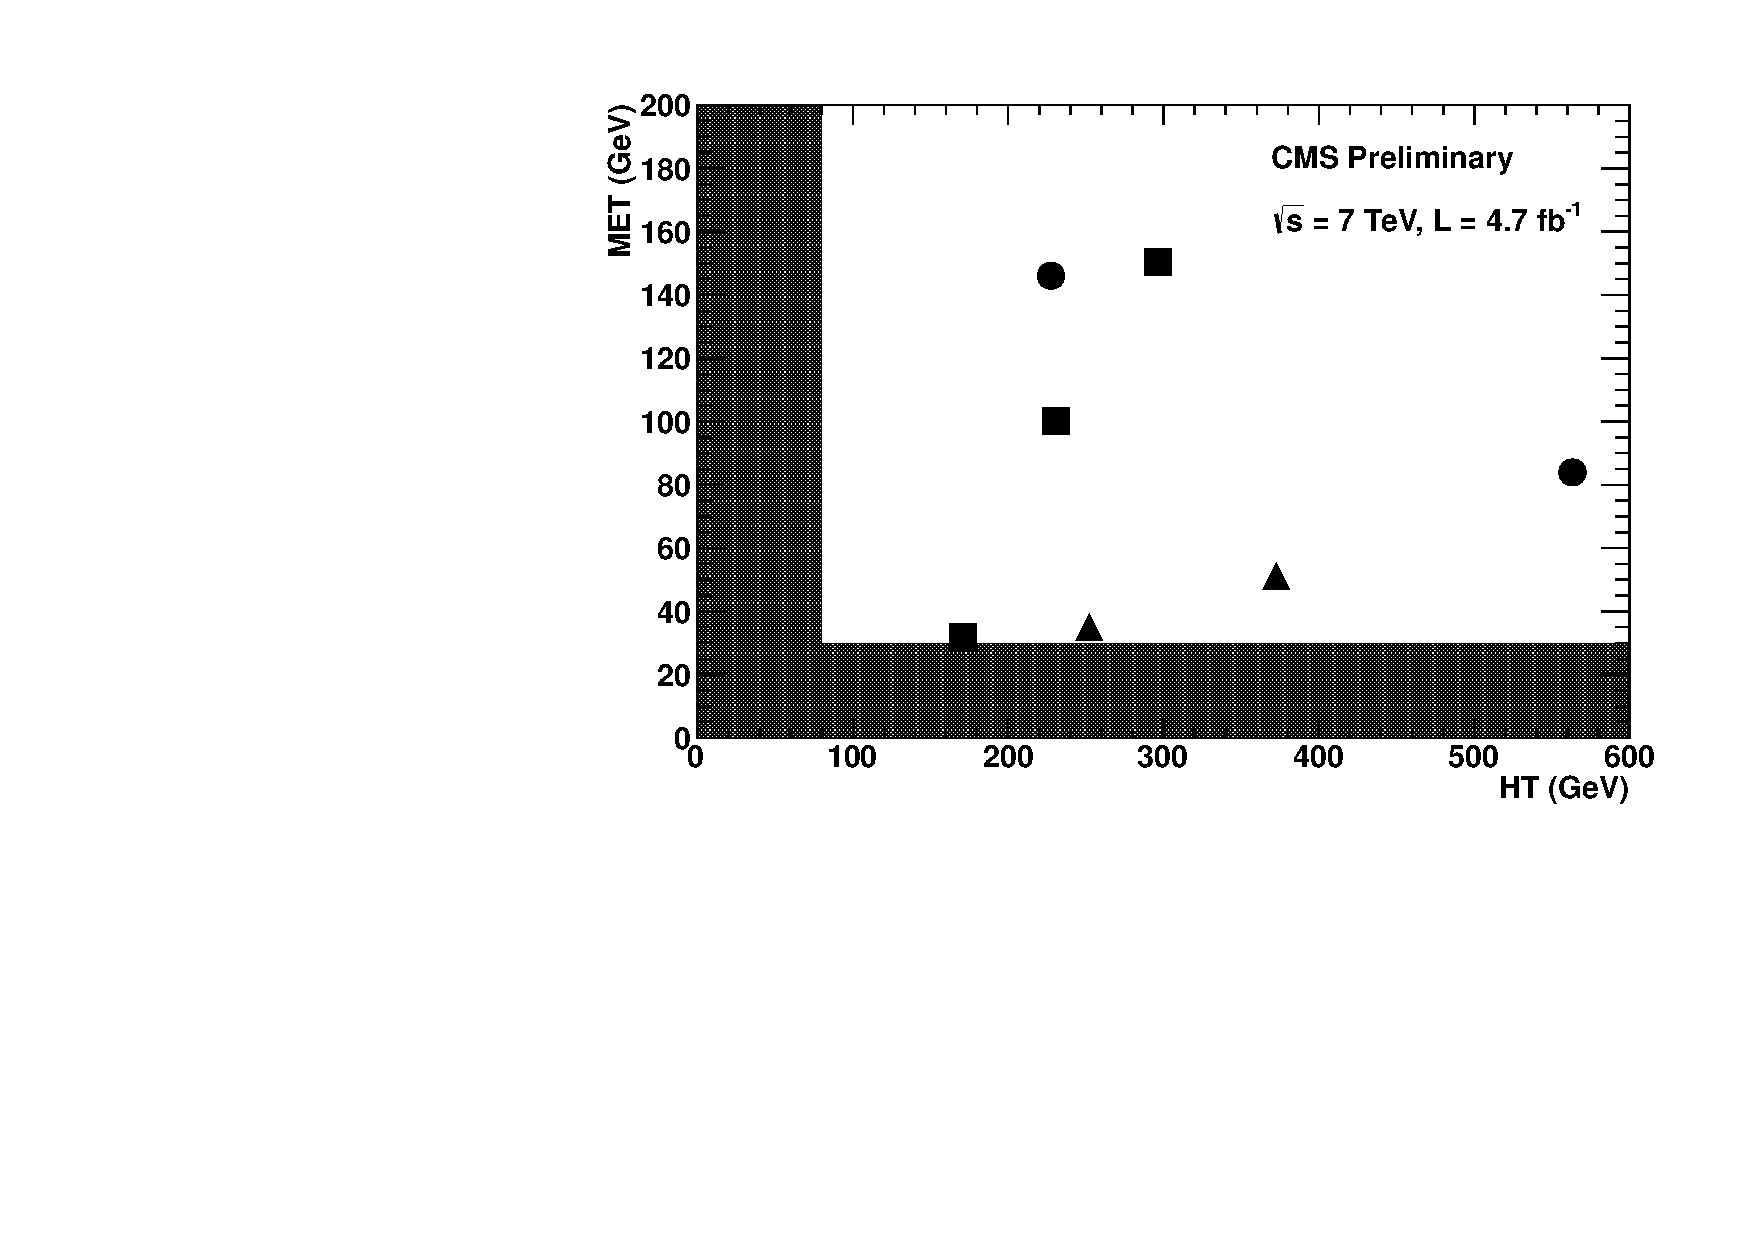
\includegraphics[width=0.48\linewidth]{figs/MetVsHt.pdf}
\caption{\label{fig:htvsmet}
Distribution of \met~~vs. $H_T$ for the 10 events in the baseline region: $H_T > 80$ GeV; $ee$ events: circles; $e\mu$ events: squares; $\mu\mu$ events: triangles.}
\end{center}
\end{figure}

\begin{figure}[h]
\begin{center}
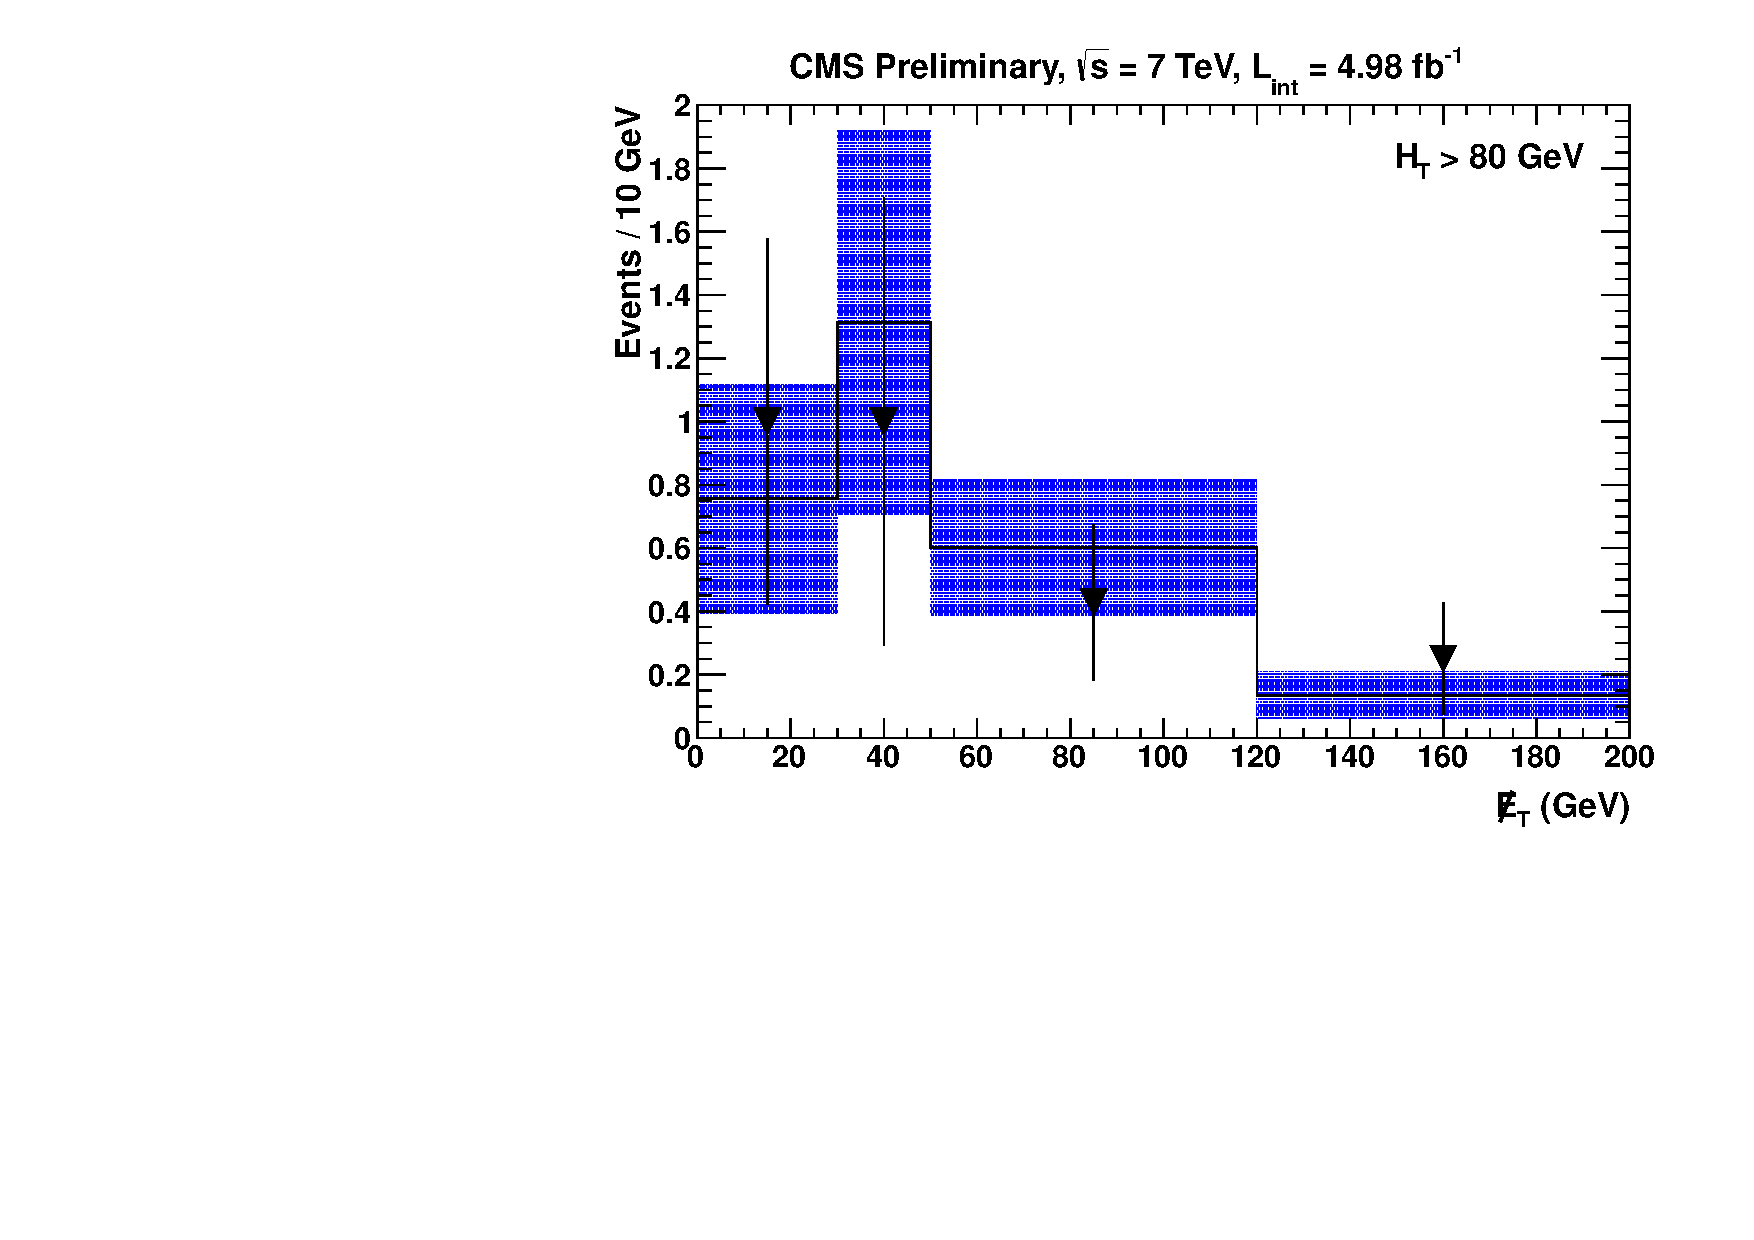
\includegraphics[width=0.48\linewidth]{figs/Met.pdf}
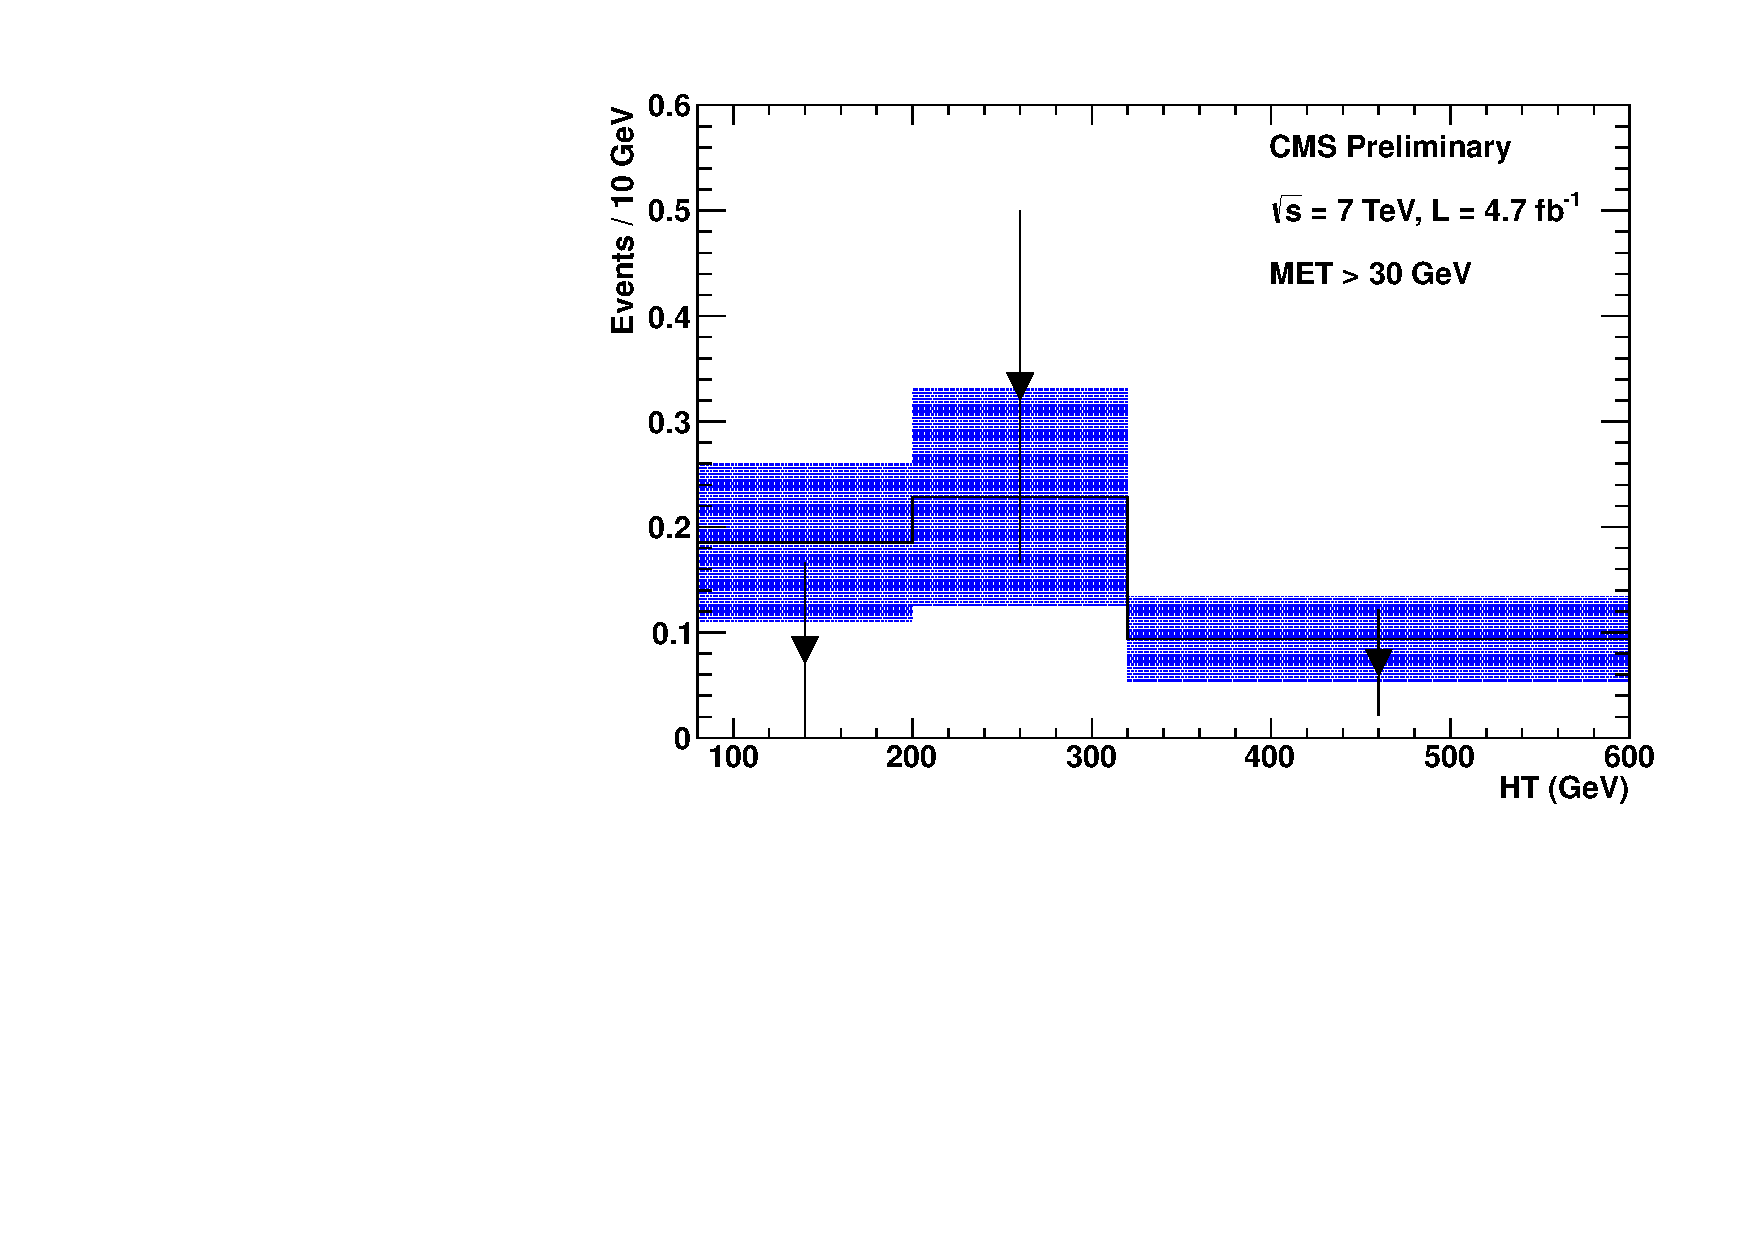
\includegraphics[width=0.48\linewidth]{figs/Ht.pdf}
\caption{\label{fig:htmet}
\met~~and $H_T$ distribution for the events in the baseline region (points).
Also shown as a histogram is the result of the background prediction.
The shading around the histogram represents the uncertainty
in the background prediction.}
\end{center}
\end{figure}


 





\section{Acceptance Systematics}
\label{sec:systematic}
Systematic uncertainties arise from uncertainties on event selections expected in simulation 
compared to the actual performance of  the detector. 
As this search is in many ways similar to the inclusive same-sign dilepton search~\cite{ssnote2011}, 
our treatment of efficiency systematics parallels the one in that analysis.
In this section, we briefly summarize those results, and
describe the uncertanities due to the b-tagging requirement.

The only new source of systematics in this analysis is from the uncertainty on the
b-jet tagging efficiency.
As already mentioned in Section~\ref{sec:bjetSF}, this uncertainty
is 4 (14)\% for jets with $\pt<240 (>240)~\GeV$.
As an illustration of the b-jet momentum distribution,
we compare them in Fig.~\ref{fig:lm9ttbar} for  \ttbar\ events (before the same-sign requirement)
and for the LM9 cMSSM SUSY benchmark point.\footnote{
The LM9 point is defined by the common scalar mass (m0) $ = 1.45$ TeV, 
the common gaugino mass (m1/2) = 175 GeV, the ratio of the Higgs expectation
values (tan$\beta)  = 10$, tri-linear coupling (A0) = 0 and the  sign of the Higgsino mass parameter ($\mu) > 0$. 
}
While most of the b-jets from \ttbar\ are below 240~\GeV, those from LM9
have a large contribution from higher momenta.
Our target searches include final states with two or more b-quark jets.
This means the efficiency to select two b-jets, as well as its uncertainty
varies among the signal final states considered
\begin{itemize}
\item same-sign top pair production, as from $Z^\prime$ exchange,
	is similar in topology to that of the opposite-sign \ttbar\ production
	and has only two b-jets in the final state with most of them with $\pt<240~\GeV$.
	The b-tagging efficiency is then approximately 10\%
	and the corresponding per-event scale factor is $0.922 \pm 0.092$.
\item direct sbottom pair production has two b-jets in the final state
	with a large fraction of b-jets with $\pt>240~\GeV$.
	The b-tagging efficiency scale factor is still 0.922, but its uncertainty
	varies among the signal model points from as low as 10\%
	to as high as 30\%.
	This uncertainty is evaluated event-by-event and then point-by-point in the limit setting procedure.
\item gluino pair production with stops in the final states considered
	here all have four b-jets in the final state.
	Now the efficiency scale factor changes as well
	depending on the number of b-jets in the acceptance.
	This is evaluated event-by-event and point-by point in the limit setting procedure.
\end{itemize}


\begin{figure}[htb]
\begin{center}
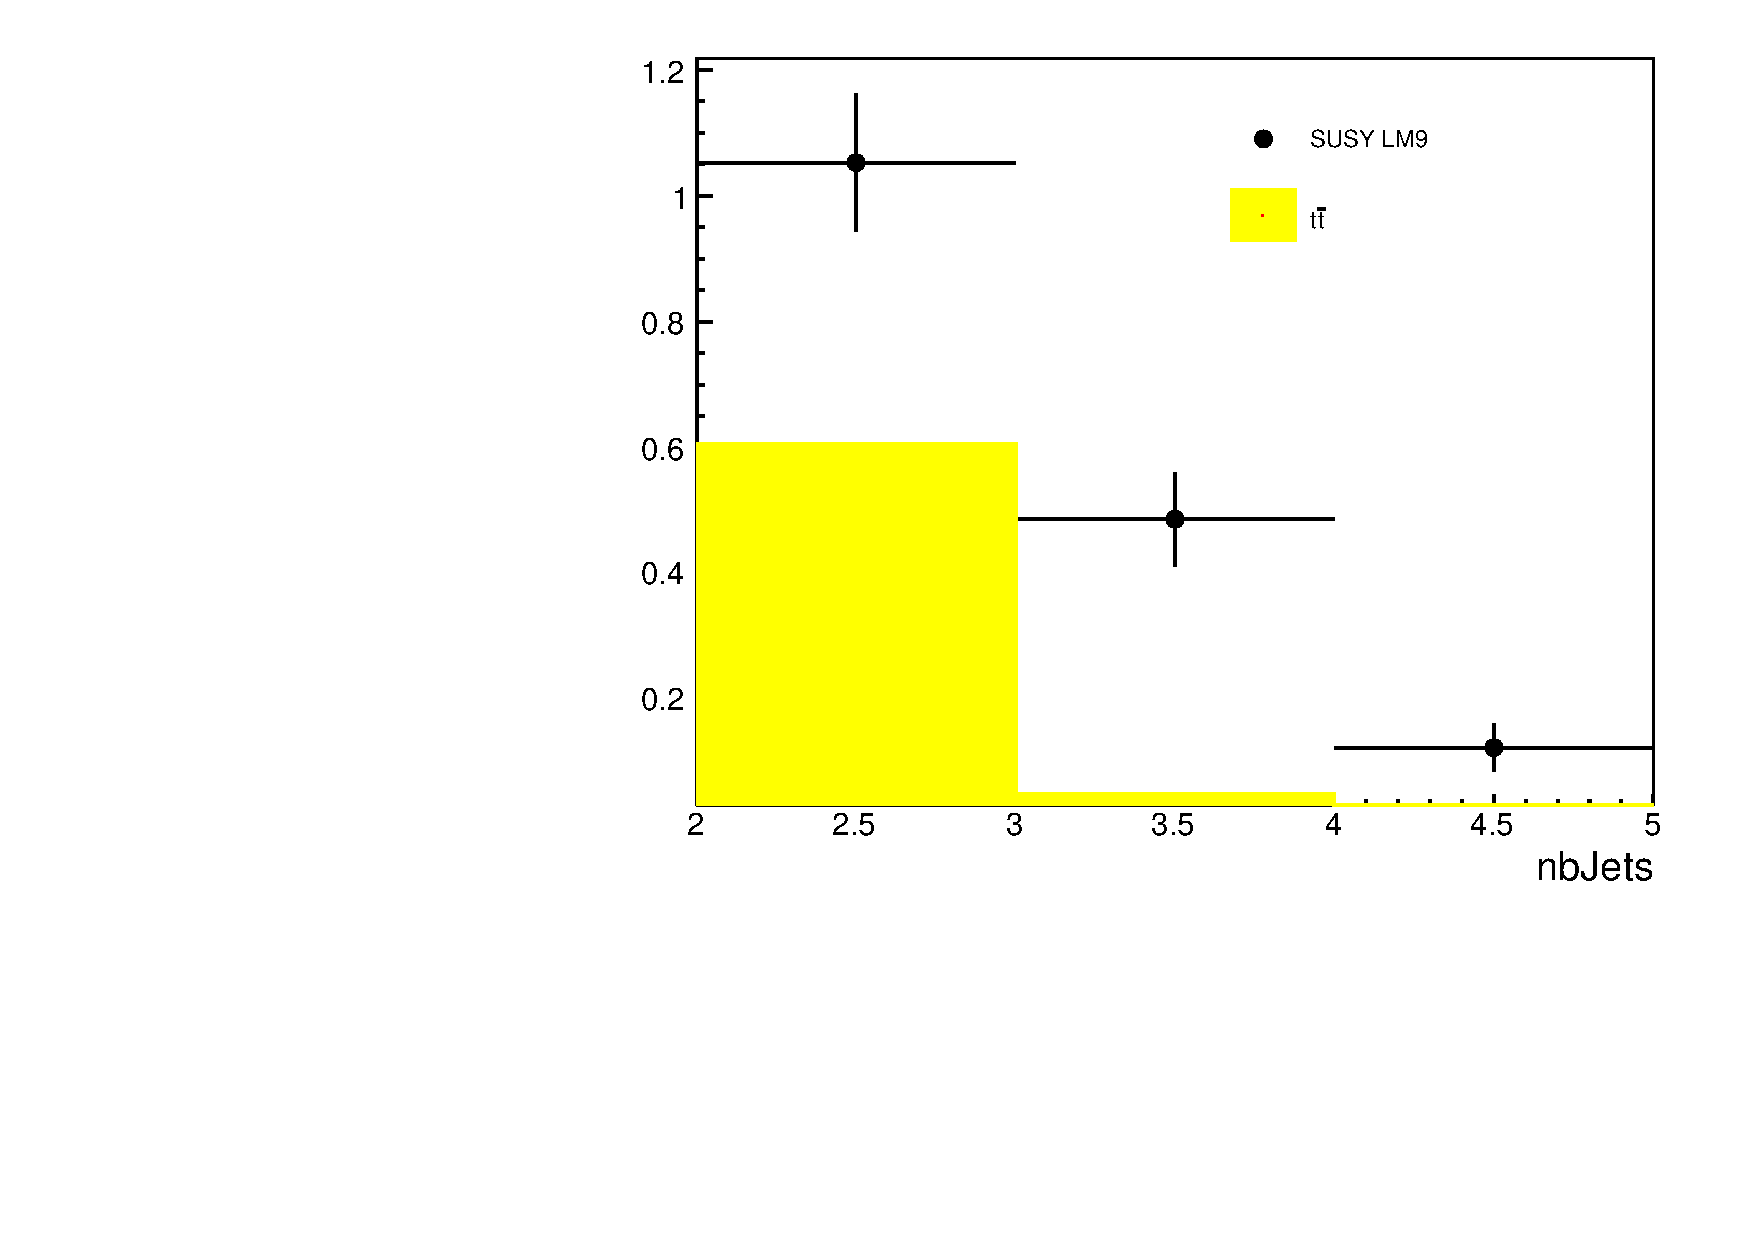
\includegraphics[width=0.48\textwidth]{figs/lm9.pdf}
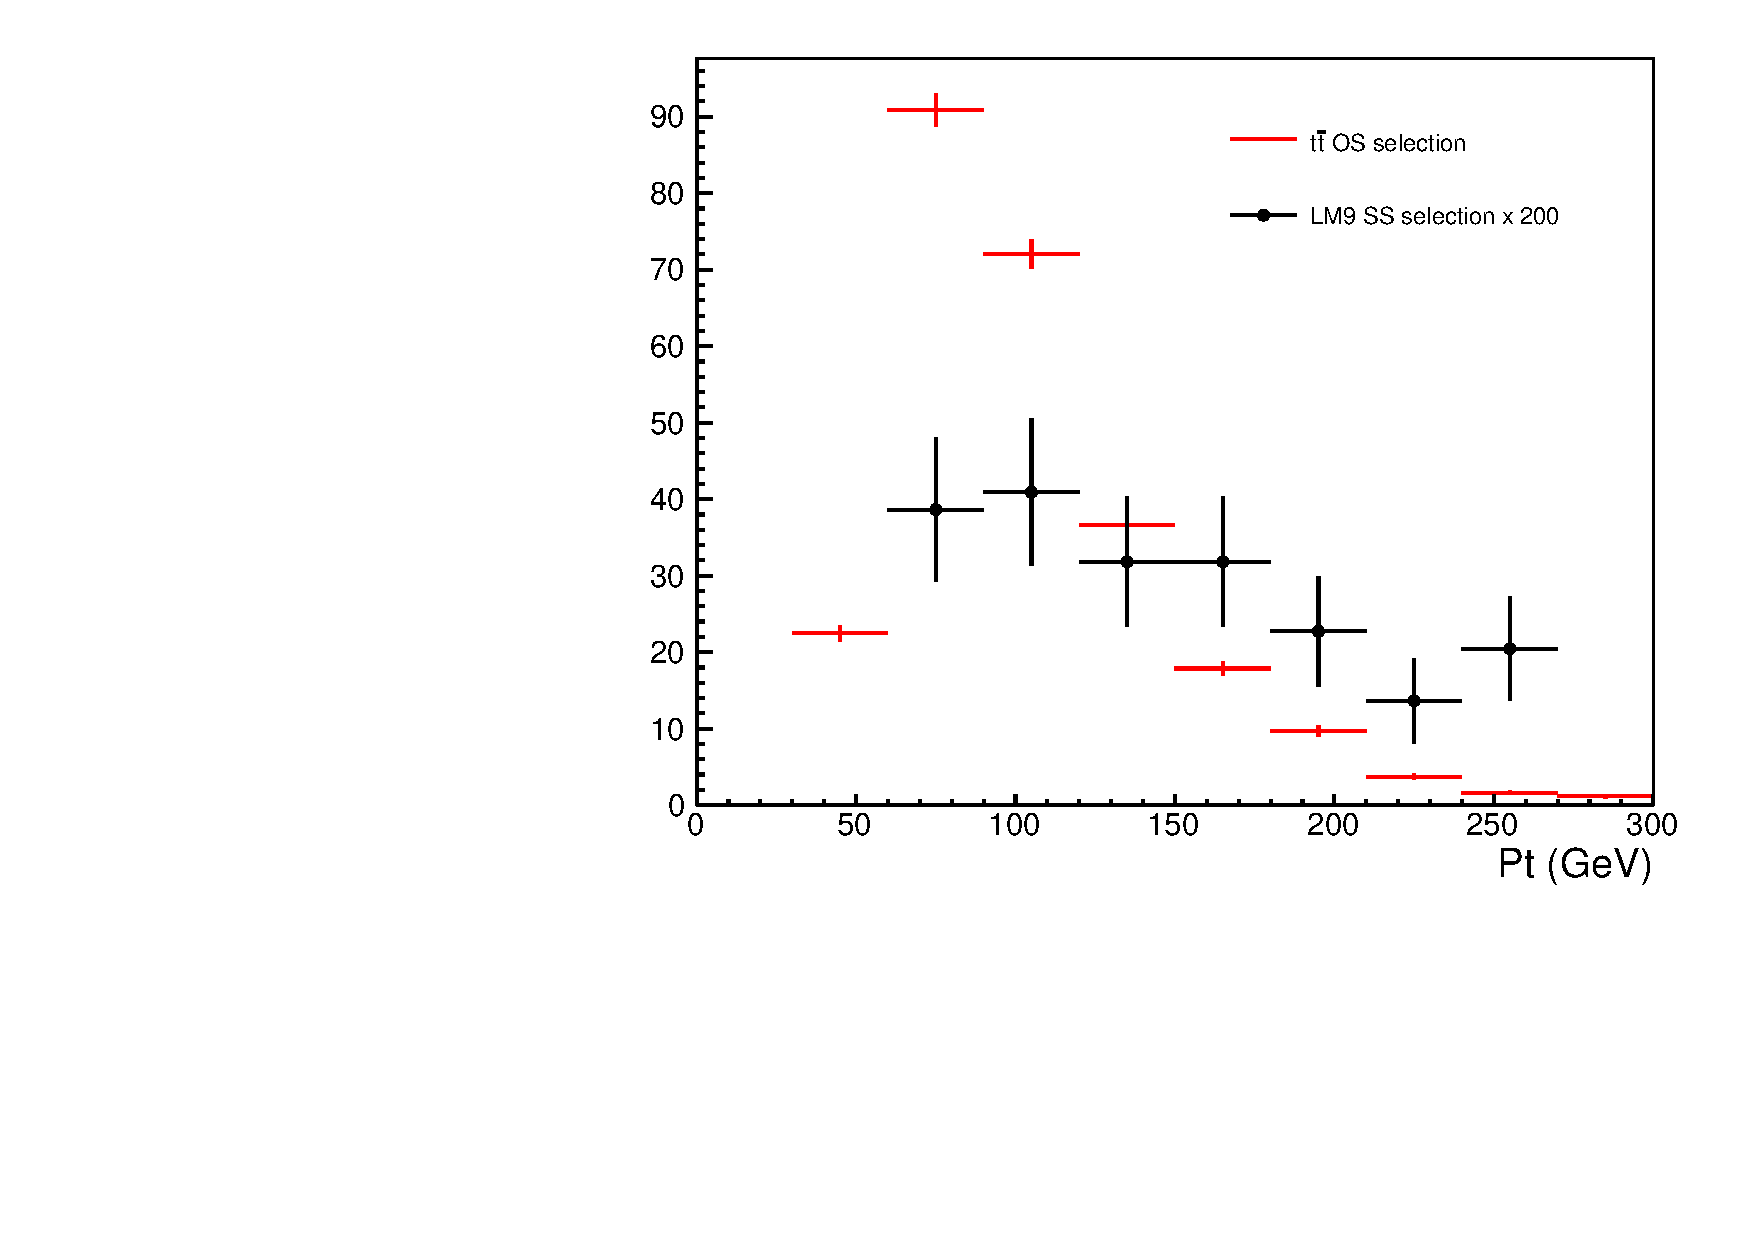
\includegraphics[width=0.48\textwidth]{figs/bjetleading.pdf}
\caption{ Differential distributions of leading b-tag jet $\pt$ for the 
LM9 benchmark point and \ttbar\ simulations.
The normalization is arbitraty.\label{fig:lm9ttbar}}
\end{center}
\end{figure}


A summary of systematic uncertainties is given in Table~\ref{tab:systSumm}.
Here the b-tagging systematics is applicable only to the same-sign top production signature.

\begin{table}[h]
\begin{center}
\caption{\small\label{tab:systSumm}Summary of systematic uncertainties on the signal selection and
expectation. 
Reported values are fractional, relative to the total cross section.
The energy scale, b-tagging, and PDF uncertainties are calculated separately in every model point.
These uncertainties quoted here are relevant to the $Z^\prime$ model.}
\begin{tabular}{lcccc}\hline
Source 					& $ee$		& $\mu\mu$		& $e\mu$	& all 	\\ \hline
Lepton selection			& 12\%		& 12\%			& 11\%		& 11\% 	\\
Energy scale				& 8\%		& 8\%			& 8\%		& 8\% 	\\
ISR/FSR and PDF				& 2\%		& 2\%			& 2\%		& 2\% 	\\
b-tag selection                         & 8\%          	& 8\%                   & 8\%           & 8\% 	\\
Total without luminosity		& 17\%		& 17\%			& 17\%		& 17\%	\\ \hline
Integrated luminosity			& 4.5\%		& 4.5\%			& 4.5\%		& 4.5\%	\\ \hline
Total 					& 17\%	 	& 17\%	 		& 17\% 		& 17\% 	\\
\hline
\end{tabular}
\end{center}
\end{table}

\subsection{Event-by-Event B-tagging scale factor and associated systematic uncertainty}
We evaluate an event-by-event btagging scale factor ($SF_{\rm event}$) as follows:

\begin{itemize}
\item for each MC event passing the event selection we start
from the scale factors $SF_i$ associated with the two or more
tagged jets.  Note that $SF_i$ can in principle be a function 
of jet $\eta$, $\pt$, etc.  Following the btag group recommendations,
for now it is taken as a constant: $SF=0.96$.

\item For events with two btagged jets: $SF_{\rm event}=SF^2$.

\item For events with three btagged jets: $SF_{\rm event}=SF^3 + 3SF^2(1-SF)$.

\item For events with four btagged jets: $SF_{\rm event}=SF^4 + 4SF^3(1-SF) + 6SF^2(1-SF)^2$.
\end{itemize}

Note that the procedure above would not work if $SF>1$, but this is not an issue
since $SF=0.96$.
It also implicitely assumes that all btags are from b-quarks.  For the models under 
consideration, we have verified that the MC contribution to the acceptance from 
events that need at least one tag from $udsgc$ in order to pass the $\ge$ 2 tags 
requirements is small.  For example, in the $Z'$ model, this contribution is
only $\approx$ 4\%.  Note that the bias in $SF_{\rm event}$ due to the improper traeatment
these events is 4\% times some quantity proportional to the difference in scale 
factors between $b$-jets and $usdgc$ jets.  Therefore, it is $<<$ 4\% and we think
can be ignored.  

In order to calculate the uncertainty ($\delta SF$) on the event-by-event $SF_{\rm total}$,
we also need the single jet btagging efficiency ($\epsilon$).  
We do not need a very precise value for $\epsilon$, since the uncertainty $\delta SF$ is 
only weakly dependent on it.  We take $\epsilon = 0.643$, independent of $\pt$
and $\eta$ for jets of $|\eta| < 2.5$.  The uncertainty on $\epsilon$ is 
the same as that on the scale factors, $\delta \epsilon = 4\% (14\%)$ (relative)
for $\pt < 240$ GeV ($> 240$ GeV).
The procedure is the following:
\begin{itemize}

\item For each event passing the requirements at RECO level, we look at the status=3 information
and we calculate the total probability ($p$) of tagging two or more jets, and 
its uncertainty ($\delta p$).

\item The calculation of $p$ and $\delta p$ is based on the number of status=3 b-quarks
of $\pt > 40$ GeV and $|\eta| < 2.5$.  

\item An event with two reconstructed btags can have $<$ 2 such status=3 b-quarks.  This 
is rare and happens for example when a 39 GeV b-quark is reconstructed as a 41 GeV
b-jet.  In these cases we calculate $p$ and $\delta p$ assuming that there are 
two 40 GeV b-quarks at status=3.

\item The uncertainty associated with the event is then $(\frac{|\delta p|}{p}) SF_{\rm event}$.

\end{itemize}

The probabilities $p$ are calculated as follows ($N$ here is the number of status=3 b-quarks
and we write the equations without the assumtion that $\epsilon$ is constant):

\begin{itemize}

\item $N=2$:~~~~$p = \epsilon_1 \epsilon_2$.

\item $N=3$:~~~~$p = \epsilon_1 \epsilon_2 + \epsilon_1 \epsilon_3 + \epsilon_2 \epsilon_3 -
2\epsilon_1 \epsilon_2 \epsilon_3$.

\item $N=4$:~~~~$$p = \prod{\epsilon_i}~~~+~~~\sum_j{(1-\epsilon_j)\prod_{i \ne j}{\epsilon_i}}
~~~+~~~\sum_{j<k}{(1-\epsilon_j)(1-\epsilon_k)\prod_{i \ne j,k}{\epsilon_i}}$$



\end{itemize}

The uncertainties $\delta p$ are calculated from the equations above assuming full 
correlation between jets, {\em e.g.}, for $N=2$ we have 
$\delta p$ = $\delta \epsilon_1 \cdot \epsilon_2 + \delta \epsilon_2 \cdot \epsilon_1$, etc.


%%\section{Results on Inlcusive Signature Search}
\label{sec:inclresults}

{\bf This section is missing two things. First, we will add a \met\ vs $H_T$ plot that shows the data and
one of the models overlayed. Second, we will add a summary of the events we see. 
}

We see 2 (1) events in the high-$p_T$ (low-$p_T$) analysis with a predicted background of
1.0$\pm$ 0.8 (0.5$\pm$ 0.7).
In absence of any significant deviation from the predicted background, we set 95\% CL. on the number of observed events. 
Two statistical methods have been used for the upper limit. 
Both methods assume the uncertainties on signal and background are un-correlated and use a log-normal distribution for error pdfs. 

The first method used to compute the upper limit is based on the Bayesian method~\cite{bayesian}.
A posterior probability $p(r)$ is used as a function of the signal strength $r = \sigma/\sigma_{SM}$ 
assuming a uniform prior for the signal strength $r$ integrating the nuisance parameters associated with the uncertainties.
The upper limit at 95\% confidence level is then determined by integrating $p(r)$ to determine $r'$, 
which satisfies $\int_{r'}^{\inf} p(r) dr = 0.05$.

We use the hybrid frequentist-bayesian $CLs$ approach~\cite{CLSxx} as the second method. 
Although the two statistical approaches are not equivalent, in this case we get similar results. 

\begin{itemize}
\item Upper limit using high-$p_T$ analysis at 95\% CL. with 24\% signal systematic error using Bayesian approach = 6.1  
\item Upper limit using high-$p_T$ analysis at 95\% CL. with 24\% signal systematic error using $CLs$ = 5.8  
\item Upper limit using low-$p_T$ analysis at 95\% CL. with 24\% signal systematic error using Bayesian approach = 4.8  
\item Upper limit using low-$p_T$ analysis at 95\% CL. with 24\% signal systematic error using $CLs$ = 4.6  
\end{itemize}

We use 6.1 and 4.8 events as the upper limit for the rest of this document for high- and low-$p_T$ analyses.



\section{Further outreach information}
\label{sec:outreach}
As mentioned in Section~\ref{sec:seleff}, we want to provide 
enough information so that anybody can use their favorite Monte Carlo
generator of new physics, define an acceptance at the hard 
scatter level (status = 3 in Pythia), and correctly estimate
the efficiency for this new physics model to within 50\% or so.

The relevant information on selection efficiencies is 
given in Section~\ref{sec:seleff}.  In this Section we give the 
second missing ingredients for this program, namely the 
95\% upper limits on the number of events for the various 
signal regions.  We also show how well our efficiency model 
works in a few cases.

\subsection{Limits on number of events}
\label{sec:outreachlimits}
In Table~\ref{tab:outreach} we summarize the 
results of the counting experiments in the various signal 
regions that are given in more 
details in Tables~\ref{tab:yield_baseline} 
to~\ref{tab:yield_ht200met503btag}; in addition, for each signal 
region we give the 95\% CL upper limit on the number of 
non-SM events ($N_{UL}$) calculated using the $CL_s$ method.

The value of $N_{UL}$ is a key ingredient to allow phenomenologists
to interpret our data: basically any model that predicts an 
event yield $> N_{UL}$ is excluded at 95\% CL.  Uncertainties 
in the efficiency need to be included in $N_{UL}$.  This is tricky 
because the components of the efficiency uncertainty associated 
with the JES and the btagging differ model-by-model.  Fortunately,
this is not a big effect.  In order to show that it is not, in 
Table~\ref{tab:outreach} we give $N_{UL}$ with uncertainties of 
12\%, 20\%, and 30\%. The first value (12\%) corresponds to the 
``minimum uncertainty'', {\em i.e.} the uncertainty due to 
lepton efficiency and luminosity only; the other two values (20\%
and 30\%) are ``typical'' uncertainty values when including
JES and btagging.


\begin{table}
\begin{tabular}{|l|c|c|c|c|c|c|c|}
\hline
 & Region 1 &  Region 2 & Region 3 & Region 4 & Region 5 & Region 6 & Region 7\\
\hline
No. of jets & $\geq 2$ &  $\geq 2$ &  $\geq 2$ &  $\geq 2$ &  $\geq 2$ &  $\geq 2$ &  $\geq 3$ \\
No. of btags & $\geq 2$ &  $\geq 2$ &  $\geq 2$ &  $\geq 2$ &  $\geq 2$ &  $\geq 2$ &  $\geq 3$ \\
Lepton charges & $++/--$ & $++$ & $++/--$ & $++/--$ & $++/--$ & $++/--$ & $++/--$ \\
\met & $\geq 30$ GeV & $\geq 30$ GeV & $\geq 120$ GeV & $\geq 50$ GeV & $\geq 50$ GeV & $\geq 120$ GeV & $\geq 50$ GeV \\
$H_T$ & $\geq 80$ GeV & $\geq 80$ GeV & $\geq 200$ GeV & $\geq 200$ GeV & $\geq 320$ GeV & $\geq 320$ GeV & $\geq 200$ GeV \\
\hline
BG from charge flips & $1.1 \pm 0.2$ & $0.5 \pm 0.1$ & $0.05 \pm 0.01$ & $0.3 \pm 0.1$ & $0.12 \pm 0.03$ & $0.026 \pm 0.009$ & $0.008 \pm 0.004$ \\ 
BG from fakes & $3.4 \pm 2.0$ &  $1.8 \pm 1.2$ &  $0.32 \pm 0.50$ &  $1.5 \pm 1.1$ &  $0.81 \pm 0.78$ &  $0.15 \pm 0.45$ &  $0.15 \pm 0.45$ \\
BG from rare SM & $3.2 \pm 1.6$ & $2.1 \pm 1.1$ & $0.56 \pm 0.28$ & $2.0 \pm 1.0$ & $1.04 \pm 0.52$ & $0.39 \pm 0.20$ & $0.11 \pm 0.06$ \\
\hline
Total expected BG  & $7.7 \pm 2.6$ & $4.4 \pm 1.6$ & $0.9 \pm 0.6$ & $3.7 \pm 1.5$ & $2.0 \pm 0.9$ & $0.6 \pm 0.5$ & $0.3 \pm 0.5$ \\
No. data events & 7 & 5 & 2 & 5 & 2 & 0 & 0 \\
\hline
$N_{UL}$ (12\% uncert.) & 7.4 & 6.9 & 5.2 & 7.3 & 4.7 & 2.8 & 2.8 \\
$N_{UL}$ (20\% uncert.) & 7.7 & 7.2 & 5.4 & 7.6 & 4.8 & 2.8 & 2.8 \\
$N_{UL}$ (30\% uncert.) & 8.1 & 7.6 & 5.8 & 8.2 & 5.1 & 2.8 & 2.8 \\ \hline \hline
$N_{UL}$ (20\% uncert.) &     &     &     &     &     &     &     \\
fakes down by factor 2  & 8.5 & 7.7 & 5.4 & 8.0 & 5.0 & 2.8 & 2.8 \\
\hline
\end{tabular}
\caption{\label{tab:outreach} A summary of the results of this search.  For each signal region,
we show its most important kinematical requirements, the prediction for the three background 
(BG) components as well as the total, the event yield, and the 95\% CL upper 
limit on the number of non-SM events in each region calculated under three different 
assumptions for the event efficiency uncertainty (see text for more details).
In the last line we show the effect of reducing the fake backgrounds
by a factor of 2, as was suggested at the preapproval presentation based
on the closure results in $t\bar{t}$ MC.  This large change in the fake background
prediction has only a small impact on the upper limits.}
\end{table}


\subsection{Testing the efficiency model}
\label{sec:outreachtest}


The efficiency model is evaluated by applying it to a few 
scenarios considered in Section~\ref{sec:stampCollecting} as
well as LM6.   
For each model, we pick a representative point
and we compare the
yield obtained by applying the full analysis selection 
in the most relevant given signal region 
to that estimated by applying the efficiencies detailed in 
Section~\ref{sec:seleff} to generator level objects.  
The results are givven below.

\begin{itemize}

\item For LM6, we tested SR4.  The parametrization was obtained on
LM6, so this is a good self-consistency check.  The efficiency
model under-predicts the acceptance by $\approx 30\%$.  This is because LM6
does not have many $b$-quarks, so mistags contribute 
significantly to the acceptance, and these are not modelled. 
When we require that b-tagged jets in simulation 
be truth matched to $b$-quarks, the agreement between 
efficiency model and simulation was at the level of 4\%.

\item For the $Z'$ model we tested SR2.  The efficiency model 
under-predicts the acceptance by $\approx 30\%$.  This was traced to 
the fact that the lepton isolation efficiency in $t\bar{t}$ (or $tt$)
events is higher than in LM6, so this effect is expected.

\item For the $\tilde{g} \to \tilde{t}t$ and {\tt T1tttt} 
models we tested SR6.
The chosen parameters where $m(\tilde{g}) = 750$ GeV, 
$m(\tilde{t}) = 380$ GeV, $m(\chi^0)=$ 50 GeV for  
$\tilde{g} \to \tilde{t}t$ and $m(\tilde{g}) = 725$ GeV, 
$m(\chi^0)=$ 75 GeV for {\tt T1tttt}.  The level 
of agreement between efficiency model and simulation was 
better than $\approx 10\%$ in both cases.

\item For sbottom pair production we tested SR1 for
$m(\tilde{b}) = 350$ GeV, $m(\chi^+)=$ 130 GeV and
$m(\chi^0)=$ 50 GeV.  The agreement was at the $5\%$
level, but the statistical precision of the test was only 
about $20\%$.

\item For $\tilde{g} \to \tilde{b}b$ we tested SR4
for $m(\tilde{g}) = 750$ GeV, 
$m(\tilde{b}) = 500$ GeV, $m(\chi^+)=$ 150 GeV, and 
$m(\chi^0)=$ 50 GeV.  Simulation and efficiency model
agreed at the 10\% level.

\end{itemize}

\noindent We consider this level of agreement to be very satisfactory.




%Figure~\ref{fig:zprimeefftest} shows the performance of the 
%efficiency model applied to the scenario of same sign top production due to t-channel exchange of a new massive $Z'$ boson.  
%The comparison was performed using the same signal region 
%considered in Section~\ref{sec:sstops}.  The estimated and actual yields agree to within 20\%.  When the mass of the $Z'$ is large compared to the mass to the top, the mass of the boson only weakly influences the kinematics of the final state so that the performance of the efficiency model is expected to be relatively constant, as observed.

%The efficiency model is evaluated by applying it to a few scenarios considered in Section~\ref{sec:stampCollecting}.  For each model considered here, points near the exclusion curve are selected and the yield obtained by applying the full analysis selection is compared to that estimated by applying the efficiencies detailed in Section~\ref{sec:seleff} to generator level objects.  Figure~\ref{fig:zprimeefftest} shows the performance of the efficiency model applied to the scenario of same sign top production due to t-channel exchange of a new massive $Z'$ boson.  The comparison was performed using the same signal region considered in Section~\ref{sec:sstops}.  The estimated and actual yields agree to within 20\%.  When the mass of the $Z'$ is large compared to the mass to the top, the mass of the boson only weakly influences the kinematics of the final state so that the performance of the efficiency model is expected to be relatively constant, as observed.

%\begin{figure}[htb]
%\begin{center}
%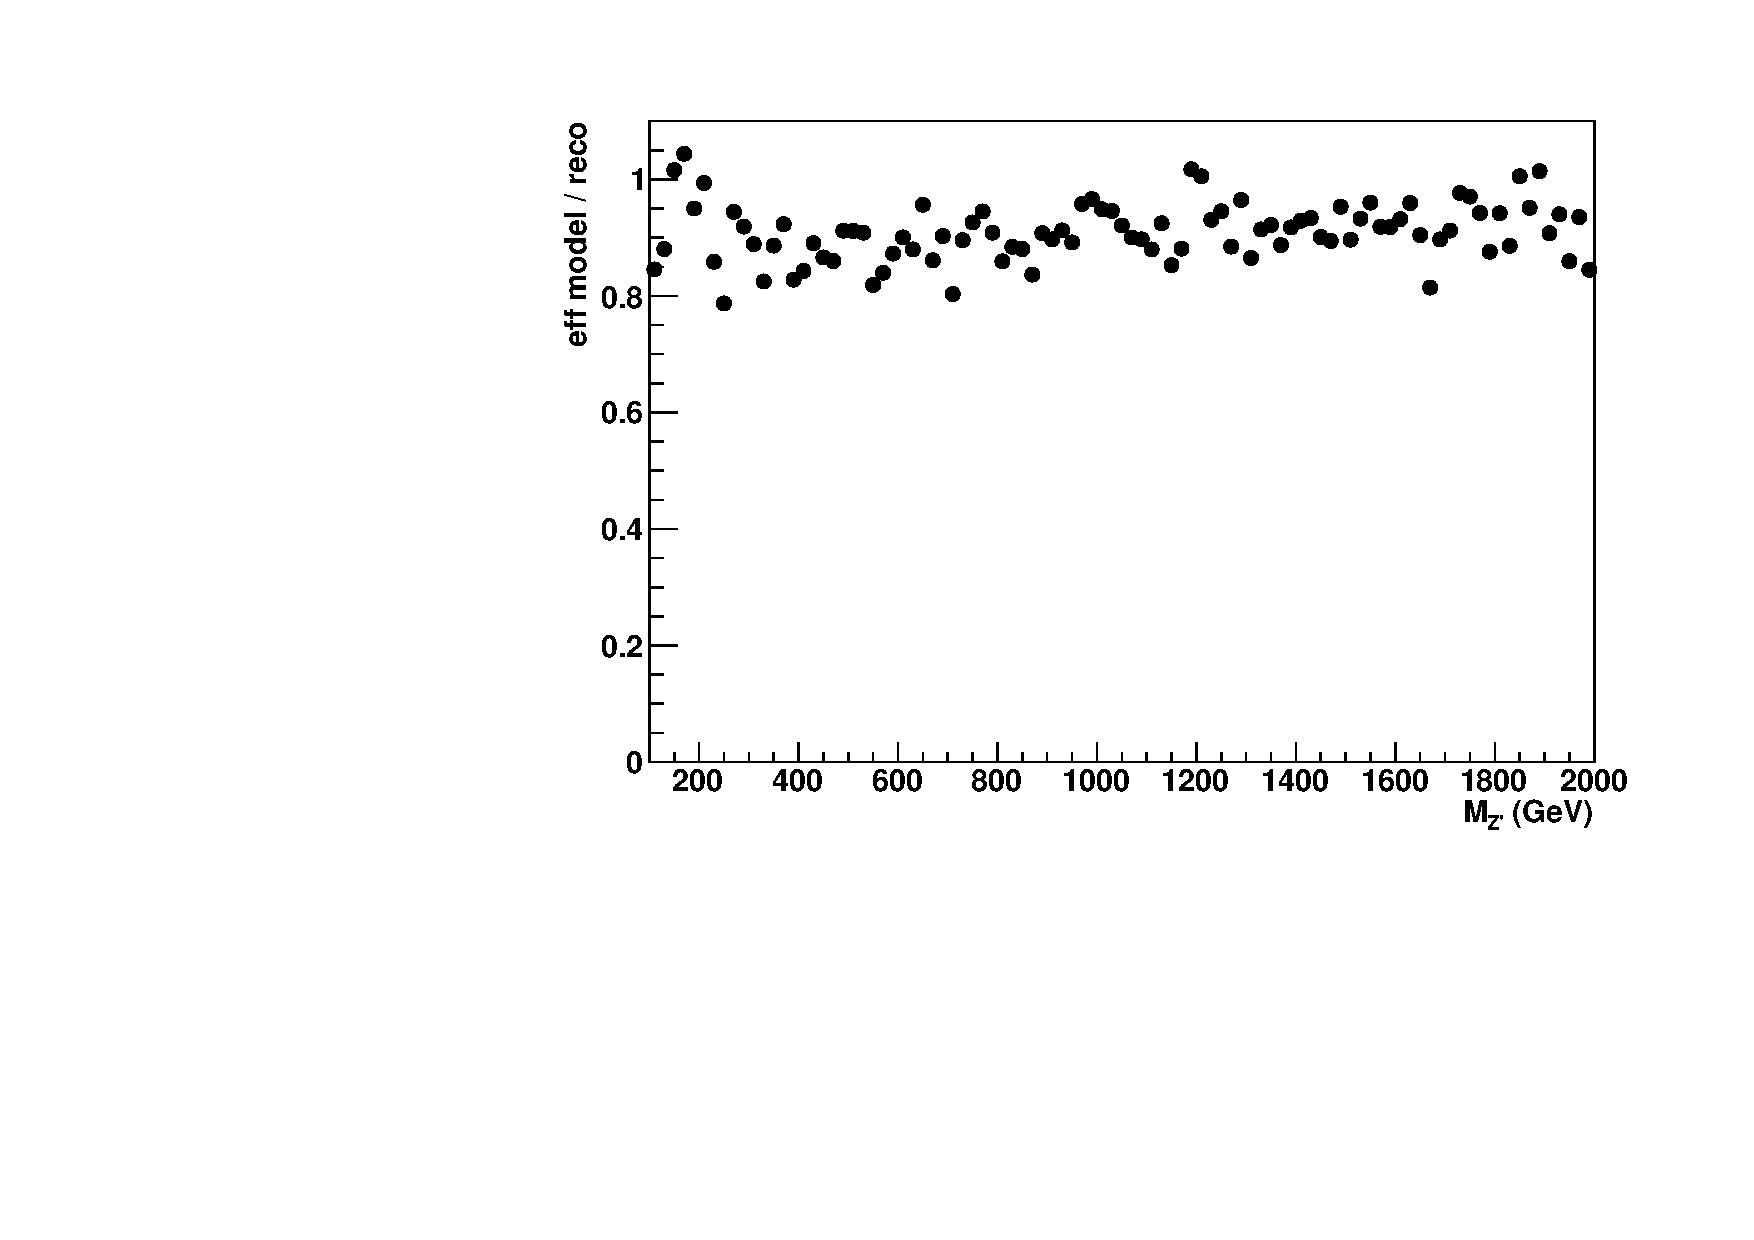
\includegraphics[width=0.95\linewidth]{figs/zprime_eff_test.pdf}
%\caption{Test of the efficiency model applied to same sign top production due to a $Z'$.  The figure shows the ratio of the yield estimated by applying the efficiency model to generator level objects to the yield obtained by applying the full analysis selection to reconstructed objects.  Estimated and actual yields agree to within 20\%.
%\label{fig:zprimeefftest}}
%\end{center}
%\end{figure}

%Several models involving stop or sbottom production were also considered in Section~\ref{sec:stampCollecting}.  As a worst case scenario, the efficiency model was tested for a few relevant points in the parameter phase space for the $\widetilde{g}$ to $t\widetilde{t}$ model.  The results of these tests are recorded in Table~\ref{tab:gluinostopefftest} .  The comparison was performed using the $\Ht > 320$ GeV, $\met > 120$ GeV signal region.  Estimated yields are found to agree with those obtained using the full analysis selection to within 50\%.

%\begin{table}
%\begin{center}
%\begin{tabular}{c | c c c}
%\hline\hline
%$m(\widetilde{g}), m(\widetilde{t})$ (GeV) & Actual Yield &  Estimated Yield & Estimated / Actual \\
%\hline
%800, 280 & 133 & 181 & 1.36 \\
%800, 430 & 125 & 184 & 1.47 \\
%650, 380 & 99 & 146 & 1.48 \\
%\hline\hline
%\end{tabular}
%\caption{\label{tab:gluinostopefftest} Test of the efficiency model applied to the $\widetilde{g}$ to $t\widetilde{t}$ model.  The table shows the ratio of the yield estimated by applying the efficiency model to generator level objects to the yield obtained by applying the full analysis selection to reconstructed objects.  Estimated and actual yields agree to within 50\%}
%\end{center}
%\end{table}
\section{Searches for Specific Models}
\label{sec:stampCollecting}

Our signature, two isolated same-sign leptons plus, at least two b-tagged jets, and \met, 
is common to many different new physics scenarios.
Here we refine our analysis to define dedicated signal regions for a few of these scenarios,
and provide 95\% C.L. upper limits on their respective model parameter space.


\subsection{Same sign top production due to a $Z'$}
\label{sec:sstops}

This is an extension of the 2010 CMS published CMS analysis\cite{sstop}.
The main difference is that here in order to improve the signal-to-noise
we require two b-tagged jets.  This would not have made sense in 2010, since 
at the time the integrated luminosity was low enough that the analysis was almost
background free without requiring b-tags.

\subsubsection{Theoretical Discussion, $Z'$ model}

Recent measurements of the inclusive forward-backward $t\bar{t}$ production 
asymmetry ($A_{FB}$) from the 
Tevatron experiments show deviations from the standard model 
(SM) expectations~\cite{d0:fwtop, cdf:fwtop1, cdf:fwtop2}.
% The largest (3$\sigma$) deviation~\cite{cdf:fwtop2} is found 
% to be in the region of high invariant mass with $M_{t\bar{t}} >  450$ GeV. 
Several attempts have been made to explain this asymmetry~\cite{fcnczprime, Buckley, Gresham, zoltan}. 
One of the most natural ways to induce such an asymmetry would be through
Flavor Changing Neutral Currents (FCNC) in the top quark sector. 
The forward-backward asymmetry in $u\bar{u} \to t\bar{t}$ would then be generated
by t-channel exchange of a new massive $Z'$ boson that couples chirally to
$u$ and $t$ at the same vertex, as shown in Fig.~\ref{fig:ttbaras}~\cite{fcnczprime}.
The same type of interaction would also give rise to same-sign top pair production, 
as illustrated in Fig.~\ref{fig:tchannel} and Fig.~\ref{fig:schannel}. 
In this case, the initial state involves two $u-$quarks and 
thus the cross section at the LHC is enhanced due 
to the large valence quark parton density of the proton. 

\begin{figure}[htb]
\begin{center}
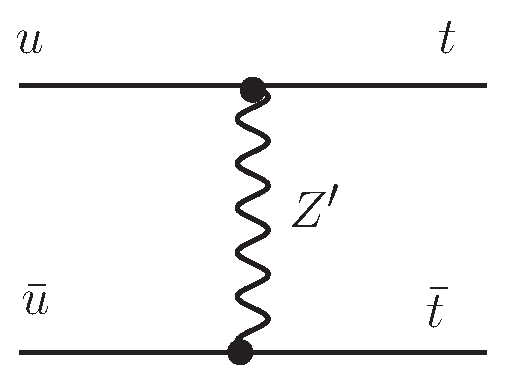
\includegraphics[width=0.35\linewidth, height=0.25\linewidth]{figs/ttbar_Z.pdf}
\caption{ Diagram for $t\bar{t}$ production induced by $Z'$ exchange which
can generate a forward-backward asymmetry. \label{fig:ttbaras}}
\end{center}
\end{figure}

\begin{figure}[htb]
\begin{center}
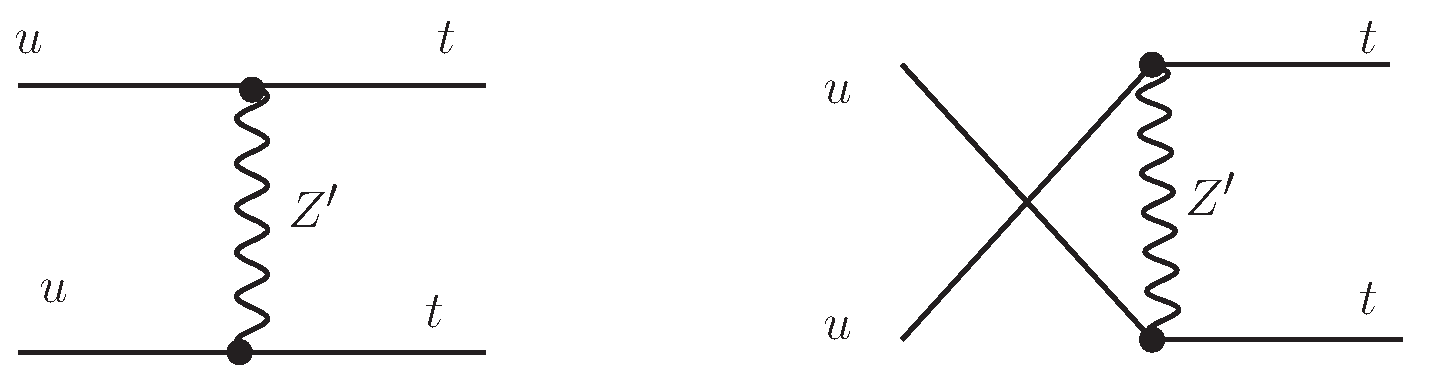
\includegraphics[width=0.7\linewidth, height=0.2\linewidth]{figs/sstop1.pdf}
\caption{ Diagrams for $tt$ pair production induced by $Z'$ exchange in the t-channel. 
\label{fig:tchannel}}
\end{center}
\end{figure}

\begin{figure}[htb]
\begin{center}
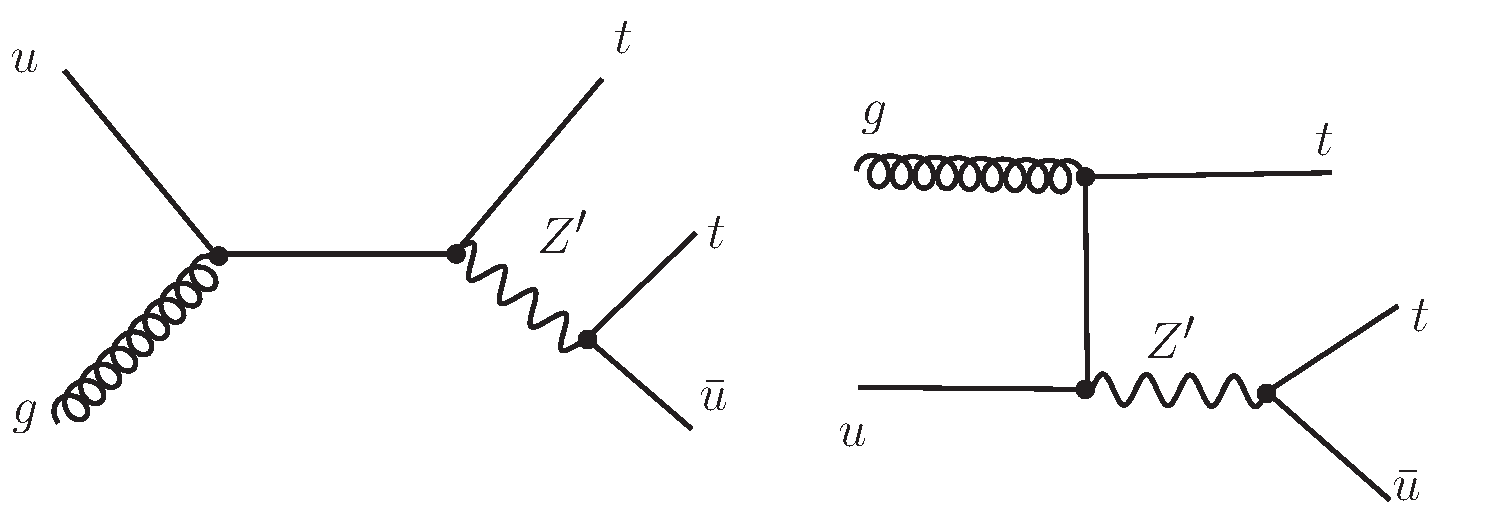
\includegraphics[width=0.7\linewidth, height=0.25\linewidth]{figs/sstop2.pdf}
\caption{ Diagrams for $tt\bar{u}$ production induced by $Z'$ exchange in the s-channel 
\label{fig:schannel}}
\end{center}
\end{figure}


We consider the model of Reference~\cite{fcnczprime}.  
The relevant $u-t-Z'$ interaction term in the Lagrangian is:

\begin{equation}
\label{eqn:L_berger}
  \mathcal{L} = g_W \bar{u} \gamma^\mu (f_L P_L + f_R P_R)tZ'_\mu + h.c
\end{equation}

where $g_W$ is the weak coupling strength. The left-handed coupling is set to $f_L = 0$, due 
to the $B_d-\bar{B_d}$ mixing constraint~\cite{Cao}. 
The right-handed coupling $f_R$ and the $Z'$ mass are free parameters in the model.
Within this model there is a narrow range of parameter space
consistent with the TeVatron measurements of $\sigma(p\bar{p} \to t\bar{t})$ 
and $A_{FB}$, which is not excluded by direct searches for same sign tops.
This region is illustrated in Fig.~\ref{fig:berger_limit}.

% Fig.~\ref{fig:tchannel} shows the t-channel exchange diagrams that can lead to the same-sign $tt$ final state. 
% As expected the coupling appears twice in the Feynman diagrams, thus the predicated rate is proportional to $f_R^4$. 

\begin{figure}[htb]
\begin{center}
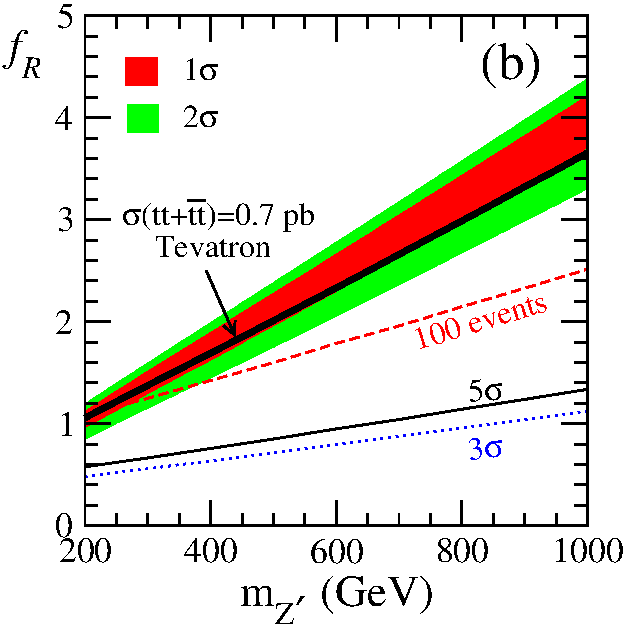
\includegraphics[width=0.4\linewidth]{figs/berger_limit.pdf}
\caption{\protect From Reference~\cite{fcnczprime}; the shaded area covers the parameter
space consistent with the $A_{FB}$ and $\sigma(t\bar{t})$ from the Tevatron;
The line indicated by the arrow shows the Tevatron limit inferred by the authors
from same sign top searches at the Tevatron; the remaining lines represent the
expectations of Reference~\cite{fcnczprime}.
for LHC searches in 1 fb$^{-1}$. \label{fig:berger_limit}}
\end{center}
\end{figure}

Monte Carlo events for this model were generated using Madgraph in the same way as 
for the 2010 analysis (see Reference~\cite{ttAN}).



\subsubsection{Signal region definition for same sign top from $Z'$}
\label{sec:sstopsigdefinition}
In this study we search for same-sign dileptons originating from $tt$ 
or $ttj$ pair production as described above.  At the LHC $uu \to tt$ 
dominates over $\bar{u}\bar{u} \to \bar{t}\bar{t}$, thus we concentrate
on same-sign positive leptons.  The \met~~and $H_T$ cuts are typical 
of a dilepton top analysis: two or more jets of $P_T>40$ GeV, 
$\met > 30$ GeV and $H_T > 80$ GeV.  This corresponds to Table~\ref{tab:yieldBase_pp}:
5 events observed and 4.42 $\pm$ 0.80 $\pm$ 1.39 expected from background.

\subsubsection{Limits on the $Z'$ model}
\label{sec:sstopslimits}
Using the results from Section~\ref{sec:sstopsigdefinition}, we set 
a limit at 95\% CL of 7.2 events using the CL$_{\rm S}$ method.
The expected limit is 6.4 events.
% $7.8^{+3.6}_{-3.1}$ events.
In the MC we find $Acc \times Eff \times BR = 0.00233$, independent of $Z'$ mass. 
This results in an upper limit on the cross-section of 0.67 pb.
The limit includes uncertainty
on JES (12\%), btagging (10\%), lepton efficiencies (11\%), luminosity (4.5\%),
and PDF (3\%).

The cross-section limit is turned into an exclusion limit in the $m(Z')$ vs $f_R$
plane using the LO calculation of the $pp \to tt$ cross-section in this model.
This is shown in Figure~\ref{fig:sstopexclusion}, together with the corresponding
plot from the 2010 analysis.  The region of parameter space favored consistent 
with the Tevatron measurements of $A_{FB}$ is excluded.


For $M_{Z'} >> M_{\rm top}$ the Lagrangian of equation 1 is 
equivalent to 
$\mathcal{L} = -\frac{1}{2}\frac{C_{RR}}{\Lambda^2}
 [\bar{u} \gamma^\mu t][\bar{u} \gamma_{\mu} t] + h.c.$~\cite{cdfth2},
with $\frac{C_{RR}}{\Lambda^2} = \frac{2 g_W^2 f_R^2}{M_{Z'}^2}$.
 Our limit on $f_R$, calculated for $M_{Z'}=2$ TeV, 
would then correspond to $\frac{C_{RR}}{\Lambda^2} < 0.6$ TeV$^{-2}$ at 
95\% confidence.  This is more stringent than the limit recently reported
by CDF: $\frac{C_{RR}}{\Lambda^2} < 3.7$ TeV$^{-2}$~\cite{cdflimit}.


\begin{figure}[htb]
\begin{center}
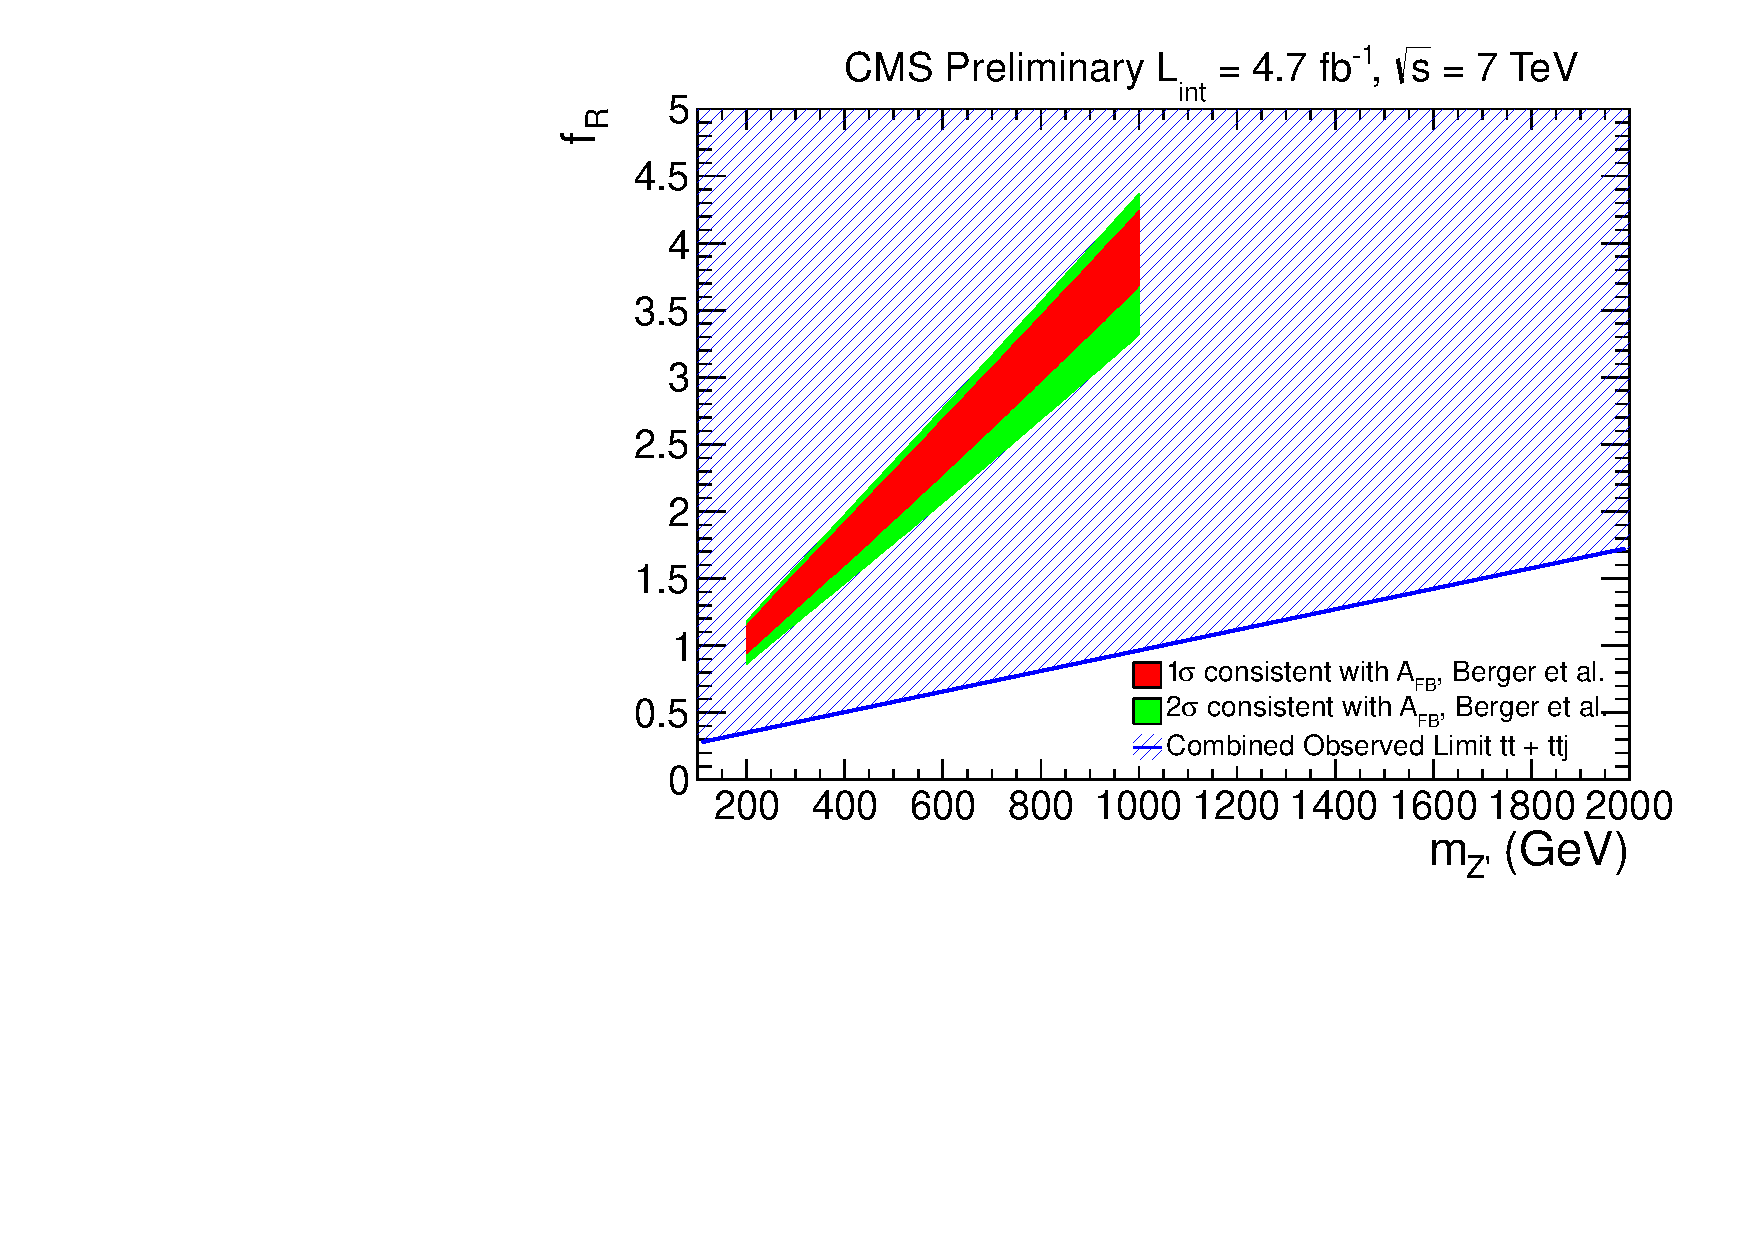
\includegraphics[width=0.45\linewidth]{figs/zprimecombined.pdf}
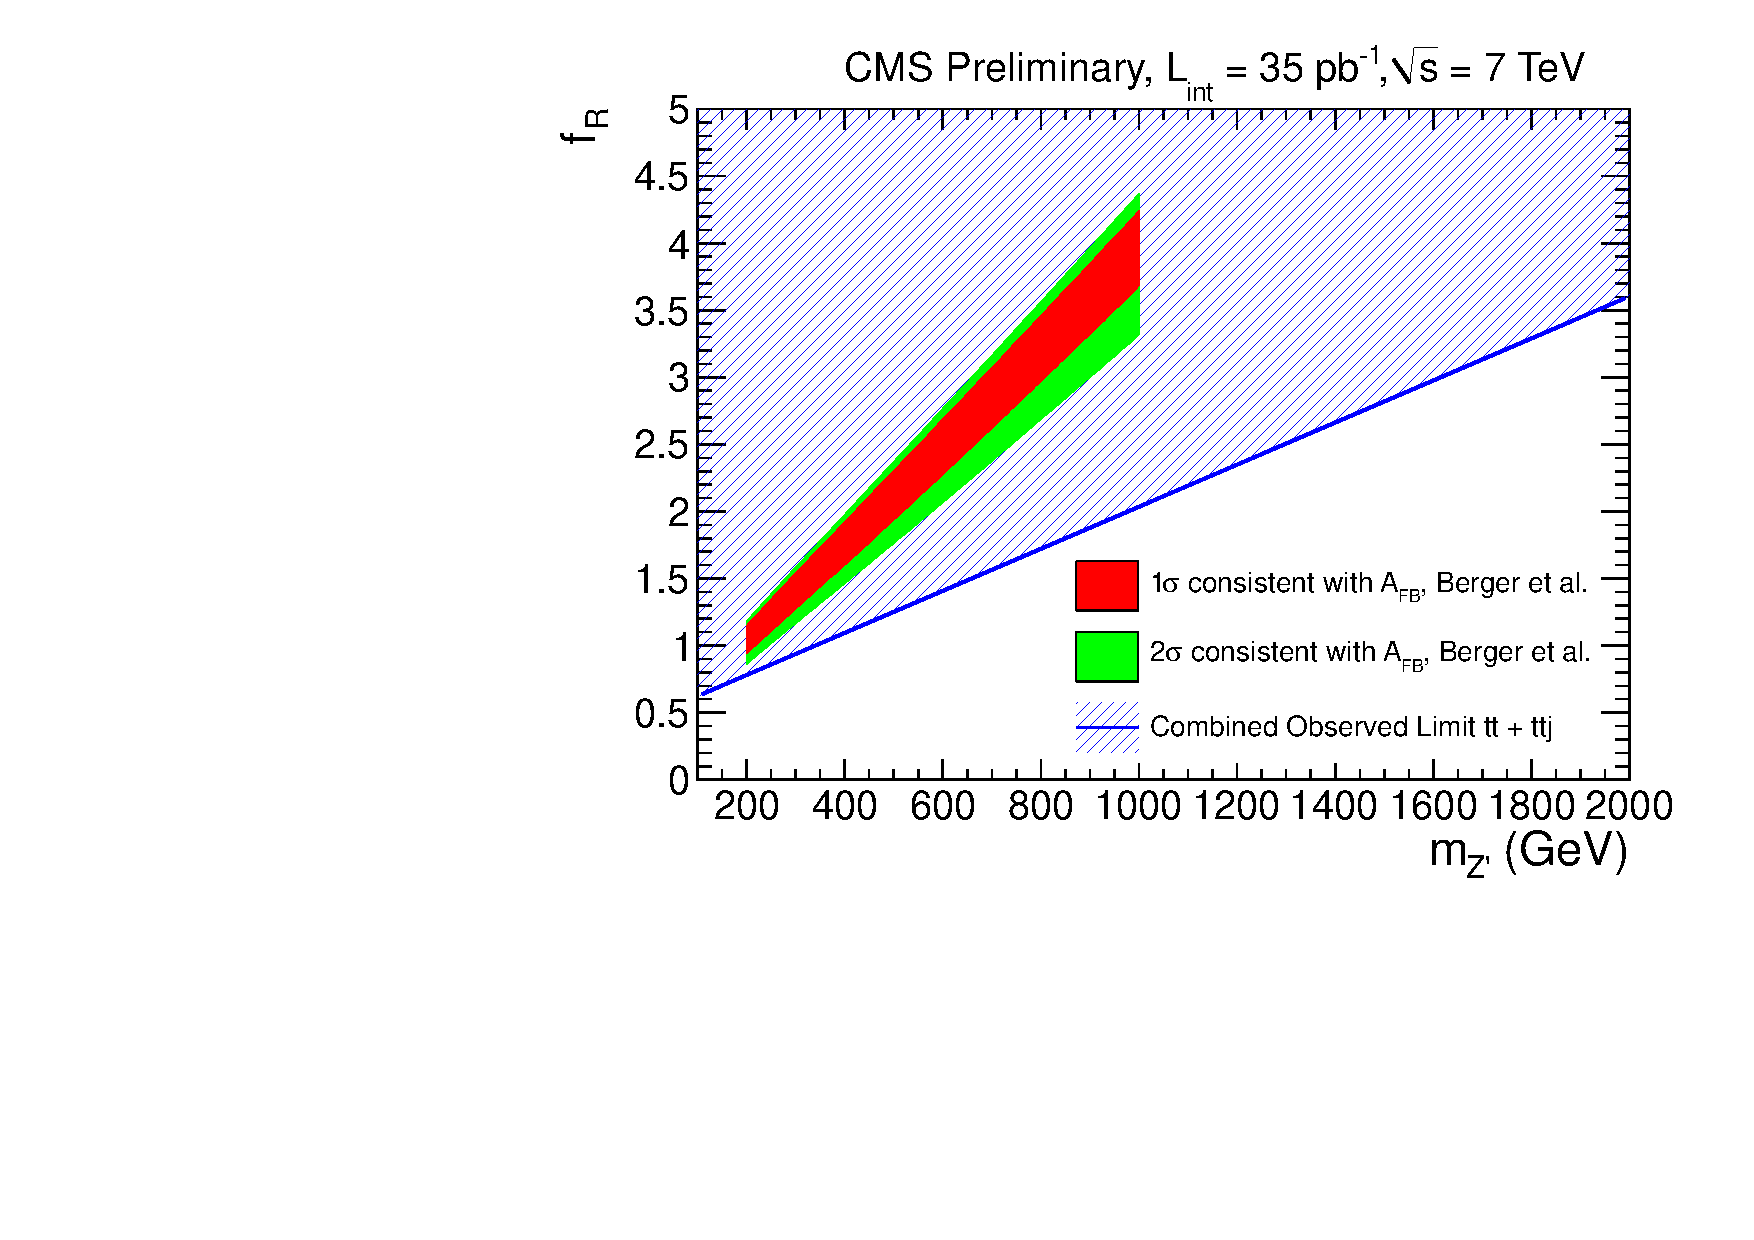
\includegraphics[width=0.45\linewidth]{figs/sscomb.pdf}
\caption{Exclusion regions from the 2011 analysis (left) and the 2010 analysis (right).
The exclusions are obtained using the LO cross-section for $tt$ production.  
Note that the cross-section is proportional to $f_R^4$.
\label{fig:sstopexclusion}}
\end{center}
\end{figure}

%\subsubsection{What is still missing for the $Z'$ model}
%\begin{itemize}
%\item Double check calculation of $\frac{C_{RR}}{\Lambda^2}$
%\item Double check acceptance numbers
%\end{itemize}


%\clearpage


\subsection{Maximally Flavor Violation Model (MXFV)}
\label{sec:mxfv}

\subsubsection{Theoretical discussion of MXFV}
\label{sec:mxfvtheory}

This is a model~\cite{mxflv1,mxflv2,mxflv3} with a new scalar 
SU(2) doublet field $\Phi_{FV} = (\eta^0,\eta^+)$ that couples the first and third 
generation quarks ($q_1,q_3$) via a Lagrangian term 
$\mathcal{L}_{FV} = \xi_{13} \Phi_{FV} q_1 q_3$.  Remarkably, it appears that this
model is largely consistent with constraints from flavor physics.

The model results in same sign top pairs in the final state as foolows
\begin{itemize}

\item Single $\eta^0$ production: $ug \to t\eta^0 \to tt\bar{u}, t\bar{t}u$

\item $\eta^0$ pair production: $u \bar{u} \to \eta^0 \eta^0 \to tt\bar{u}\bar{u},
uu\bar{t}\bar{t}, t\bar{t}u\bar{u}$

\item $\eta^0$ $t$-channel exchange: $uu \to tt$, $\bar{u}\bar{u} \to \bar{t}\bar{t}$
\end{itemize}

Monte Carlo events were generated using LHE files\cite{simplifiedModel} interfaced 
with Madgraph.  Madgraph was used to decay the top quarks in order to preserve 
spin-correlations.  The cross-sections at LO for same sign $tt$ pairs for the three
processes in the MXFV model is shown in Figure~\ref{fig:mxvxsec}.  The $t$-channel
process is the dominant for $\xi = 1$.  At smaller values of $\xi$, 
$ug \to \eta^0 \to tt\bar{u}$ becomes more important, since its cross-section 
varies as $\xi^2$, while in the $t$-channel case it goes as $\xi^4$.

\begin{figure}[htb]
\begin{center}
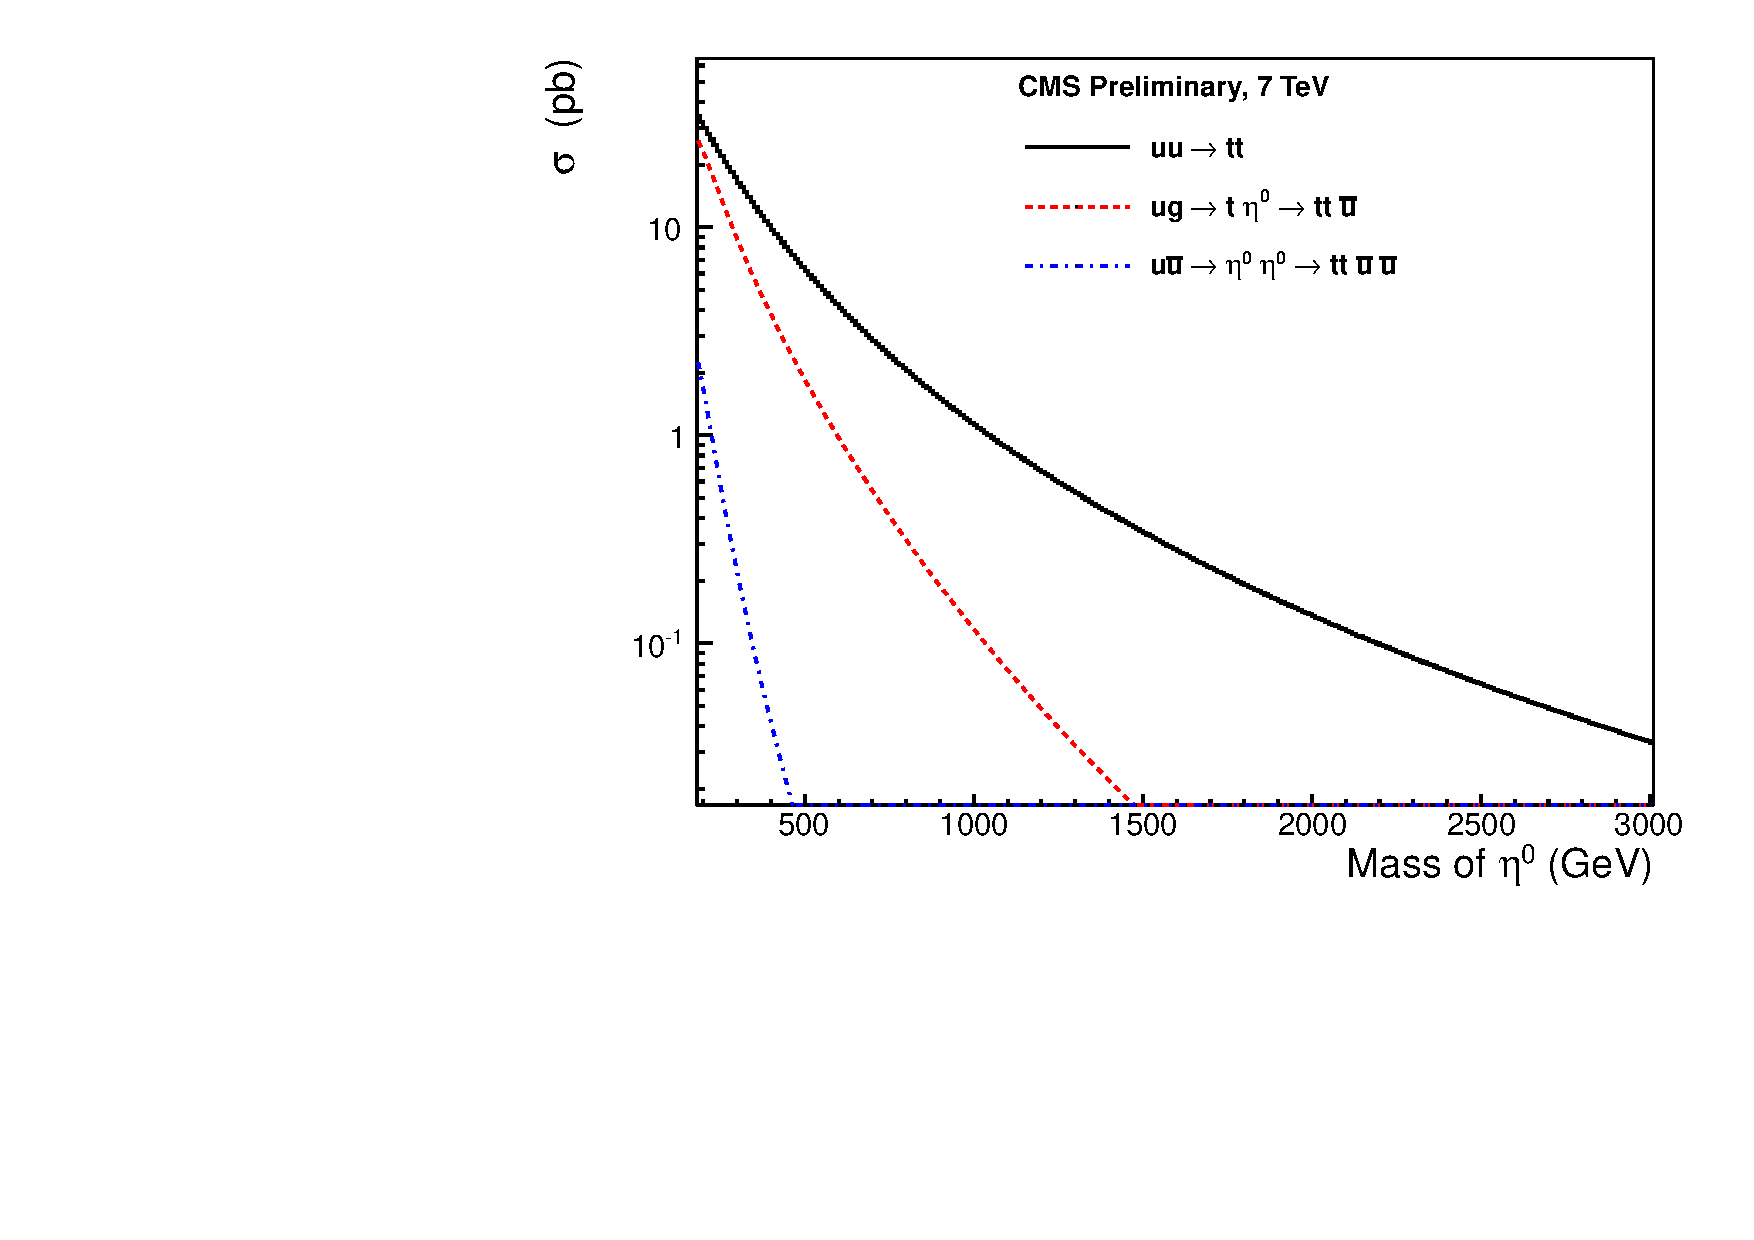
\includegraphics[width=0.55\linewidth]{figs/mxvxsec.pdf}
\caption{Cross section at LO for the $tt$ final state in the three MXFV modes
as a function of $\eta^0$ mass for $\xi = 1$.
\label{fig:mxvxsec}}
\end{center}
\end{figure}

\subsubsection{Signal region definition for the MXFV model}
\label{sec:mxfvdefinition}
The properties of the final state in this model are basically the same as in the $Z'$ model.
Thus, we use the same signal region definition (see Section \ref{sec:sstopsigdefinition}).


\subsubsection{Limits for the MXFV model}
\label{sec:mxfvlimits}
Our limits in the $\xi$-M($\eta^0$) plane are shown in 
Figure~\ref{fig:MxVExcl}.
They are calculated using the LO cross-section for this model.

\begin{figure}[htb]
\begin{center}
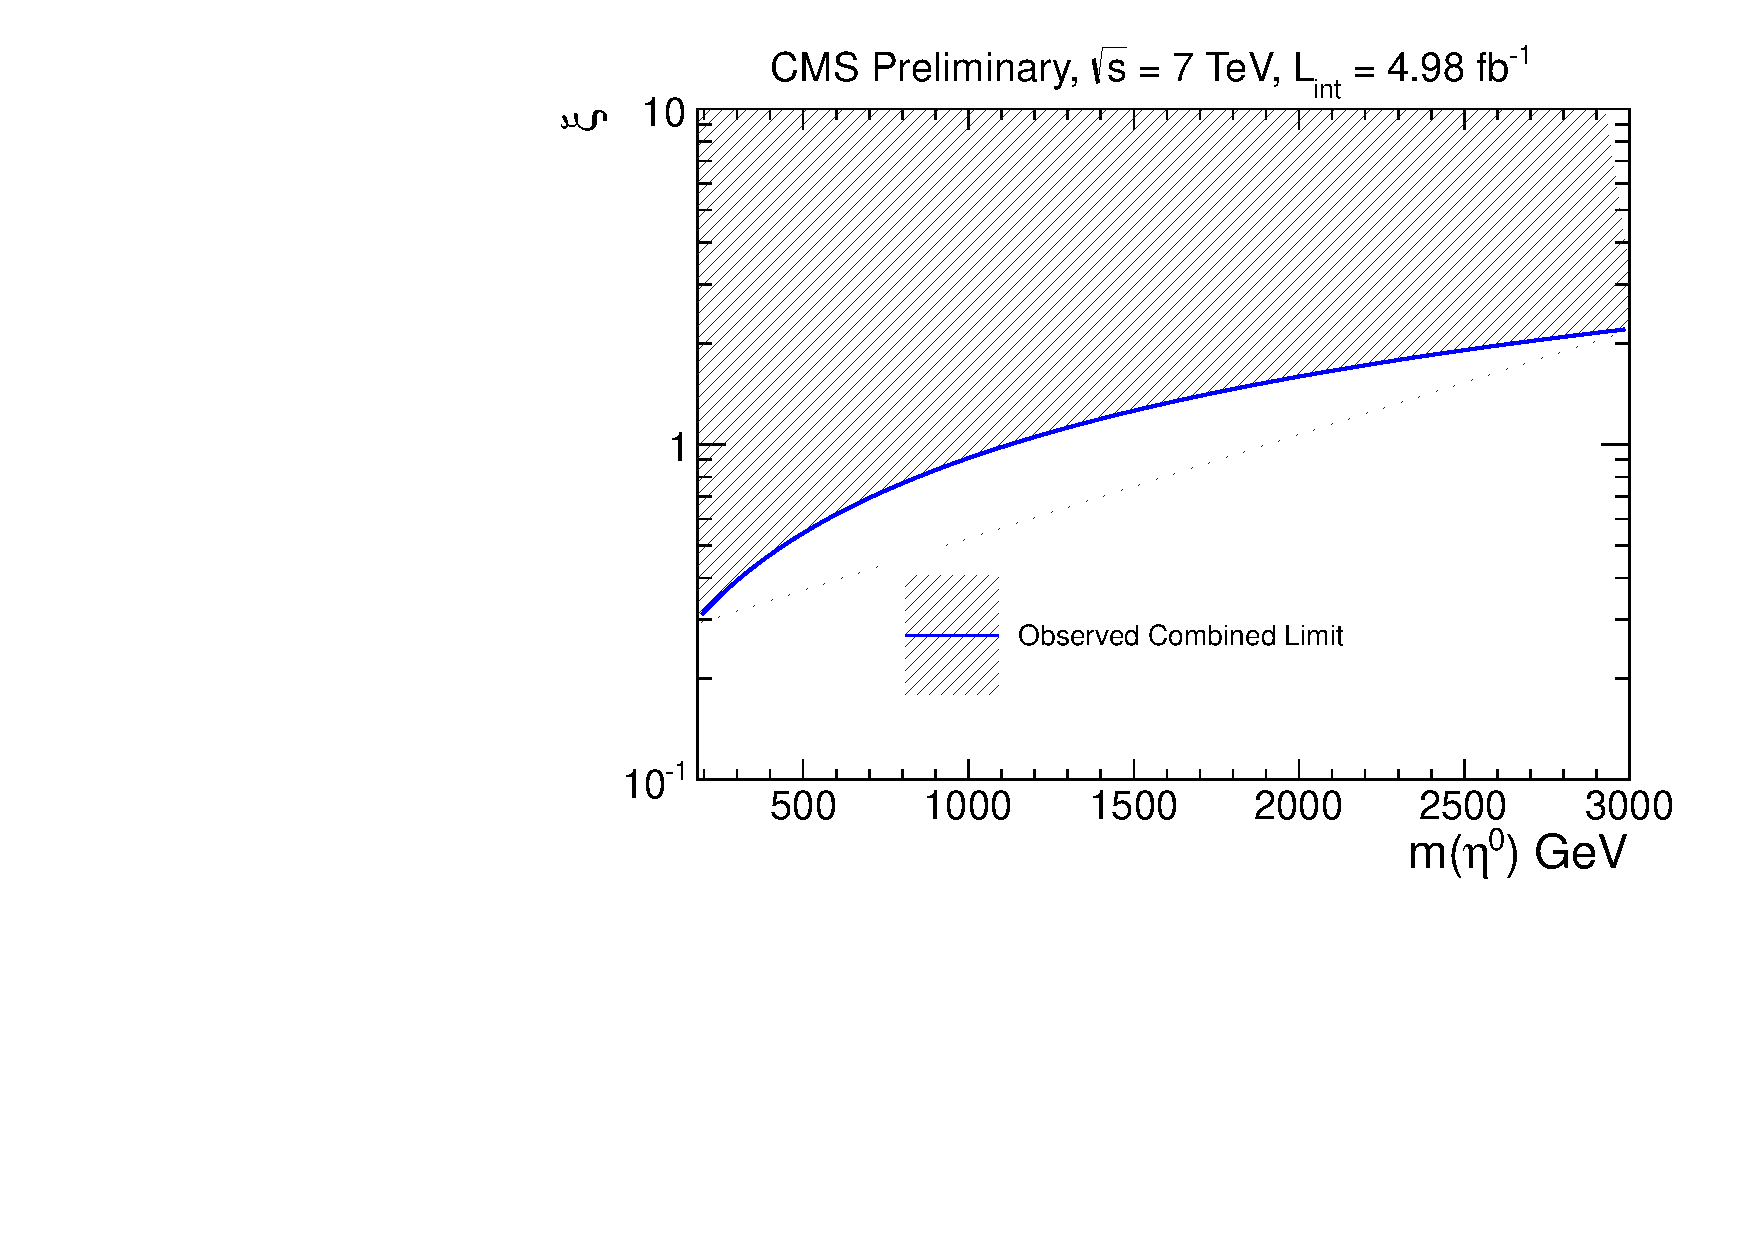
\includegraphics[width=0.45\linewidth]{figs/MxVExclCombined.pdf}
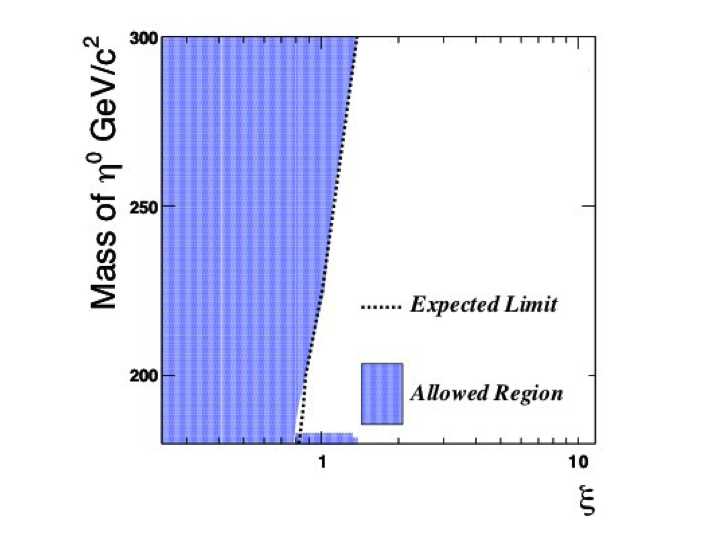
\includegraphics[width=0.45\linewidth]{figs/CDFlimit.png}
\caption{Limits in the $\xi$-Mass($\chi^0$) plane.  Left: CMS.  Right: CDF
\label{fig:MxVExcl}}
\end{center}
\end{figure}

%\subsubsection{What is still missing for the MXFV model}
%\begin{itemize}
%\item Need to include the $tt\bar{u}$ final state
%\item Rescale everything to take into account that the leptonic BR in MG is not quite right
%\item Signal Contamination effects (should be tiny)
%\item Prettify the exclusion plot, put CDF on same plot perhaps
%\end{itemize}



\subsection{$\widetilde{g} \to t\widetilde{t}$ Model}
\label{sec:firststopmodel}

\subsubsection{Theoretical discussion of the $\widetilde{g} \to t\widetilde{t}$ Model}
\label{sec:firststopmodeltheory}

This is an interesting model for stop pair production through gluino 
decays\cite{susyssbtags}\cite{susyssbtags2}\cite{wacker}\cite{naturalness4}.
It is a ``realistic'' and well-motivated 
model in the sense that it applies to the situation 
where all the squarks except the stop are very heavy.  A ``light'' stop is of course
generally favored in SUSY, and LHC results are pointing to ``heavy'' superpartners.
Then if the stop
is light enough the gluino would decay with 100\% BR as $\widetilde{g} \to t\widetilde{t}$
and then the stop would decay as $\widetilde{t} \to t \chi_1^0$, if kinematically 
accessible.
The parameters of the model are $M(\widetilde{g})$, $M(\widetilde{t})$, $M(\chi_1^0)$.

The final state after gluino pair production is then $tt\bar{t}\bar{t}\chi_1^0\chi_1^0$.
It is the same final state as the {\tt T1tttt} 
simplified model\cite{T1tttt}, except that 
it proceeds through an intermediate on-shell stop.  This final state is rich in leptons,
and has four b-quarks.  The same sign dilepton $+$ btags $+$ 
\met~~signature is a 
particularly good way to go after it.


\subsubsection{Signal region definition for the $\widetilde{g} \to t\widetilde{t}$ Model}
\label{sec:firststopdefinition}

\begin{figure}[htb]
\begin{center}
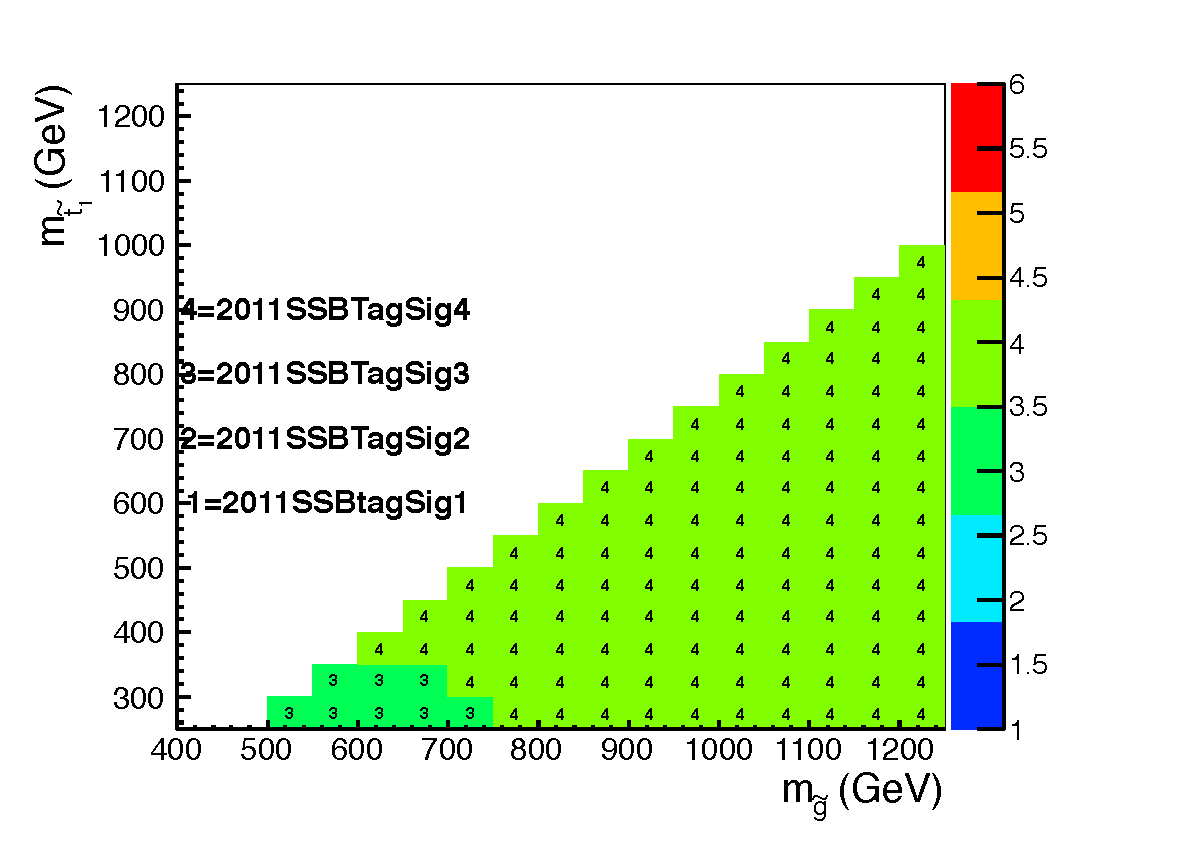
\includegraphics[width=0.65\linewidth]{figs/gluinostopsigreg.pdf}
\caption{The signal region with the best expected limit as a function of 
$m(\widetilde{g}$ vs. $m(\widetilde{t})$ plane for $m(\chi^0_1)$=50 GeV.
The coding is: 1=(200-50), 2=(200-150), 3=(320-50), and 4=(320-120), where
the first (second) number is the $H_T$ (\met) threshold in GeV. The number
of requested btags is 2 or more.
\label{fig:gluinostoptimize}}
\end{center}
\end{figure}


For each point in parameter space we use the signal region that gives
the best expected limit.  
{\bf (Note: so far the region with 3 btags has not been used).}
Limits are calculated using all experimental
uncertainties; the JES and btag uncertainties are calculated point-by-point.
An example of this optimization is shown in Figure~\ref{fig:gluinostoptimize},
where we show the choice of signal region that gives the best expected limit
in the $m(\widetilde{g})$ vs. $m(\widetilde{t})$ plane for the choice
$m(\chi^0_1)$=50 GeV.



%Using $\met > 50$ GeV and $H_T > 200$ GeV, which corresponds 
%to Table~\ref{tab:yield_ht200met50}: 5 events observed and 3.723 $\pm$ 0.787 $\pm$ 1.23 expected from backgrounds,
%we set a limit at 95\% CL of 7.65 events with the  CL$_{\rm S}$ method. The expected limit is 6.13. 

\subsubsection{Limits for the $\widetilde{g} \to t\widetilde{t}$ Model}
\label{sec:firststoplimits}



The limits on the production cross-section in this model in the 
gluino mass vs. stop mass plane for two choices of the 
LSP mass are shown in Figure~\ref{fig:mglinoStop}
Using the 
NLO$+$NLL cross-section for gluino pair production, we also place a limit
on the mass parameters of this model.  We basicaly can exclude 
$m(\widetilde{g})$ up to about 800 GeV for all kinematically allowed
values of the stop mass: 
$m(t)+m(\chi^0_1)~<~m(\widetilde{t})~<~m(\widetilde{g})-m(t)$. 



\begin{figure}[htb]
\begin{center}
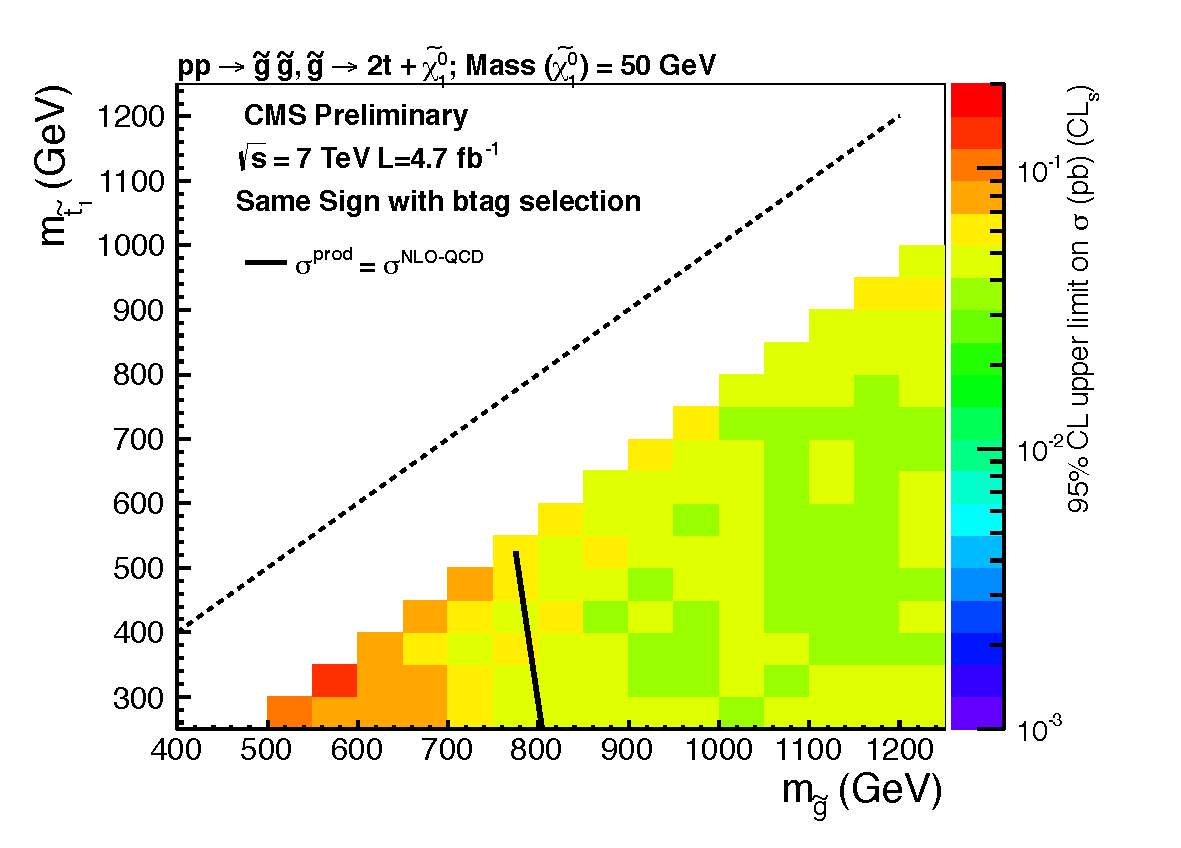
\includegraphics[width=0.47\linewidth]{figs/gluinostop50.pdf}
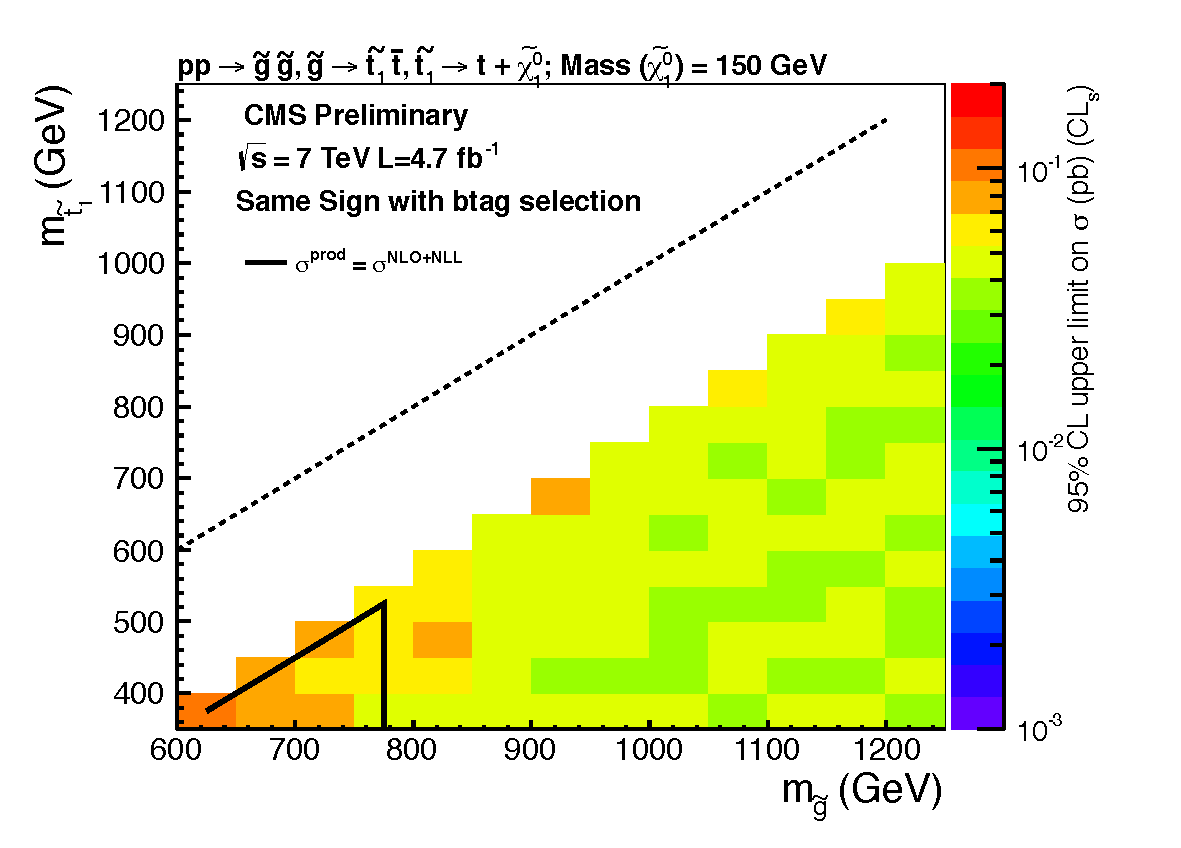
\includegraphics[width=0.47\linewidth]{figs/gluinostop150.pdf}
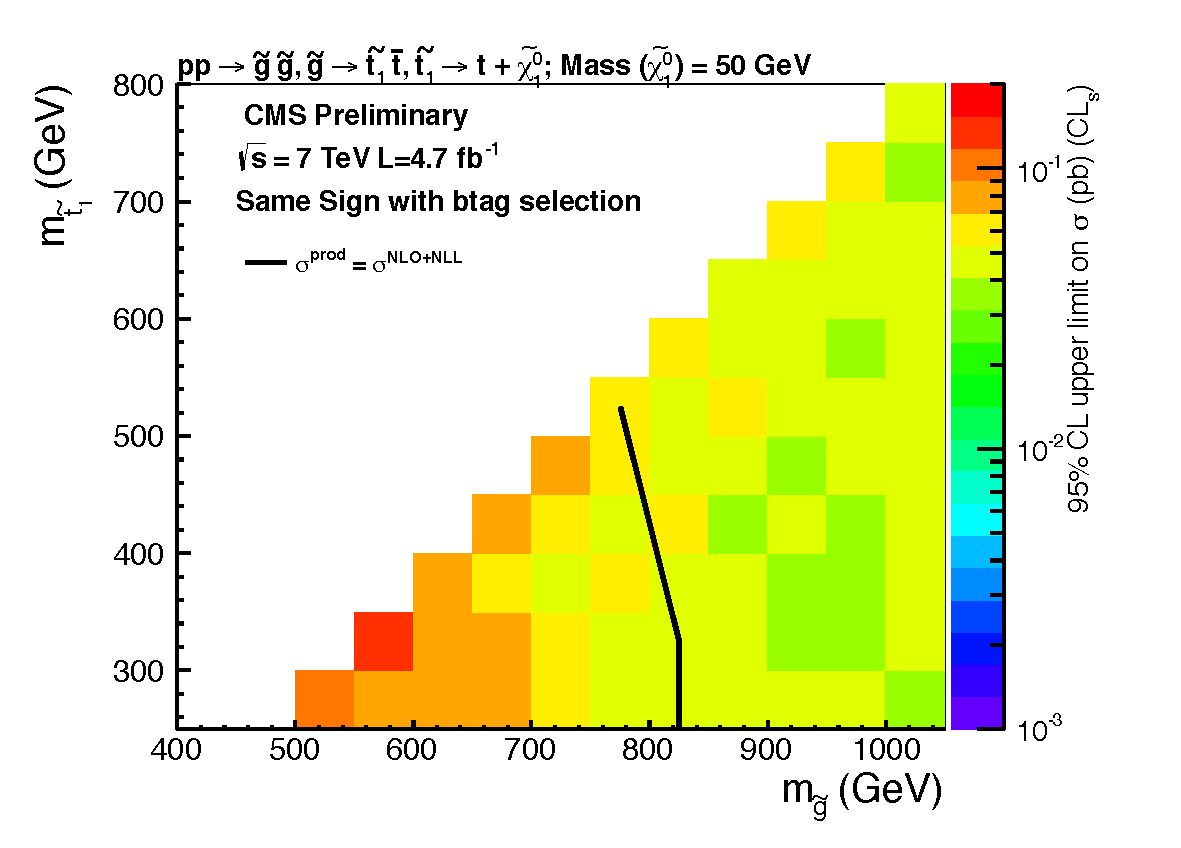
\includegraphics[width=0.47\linewidth]{figs/gluinostop50_zoom.pdf}
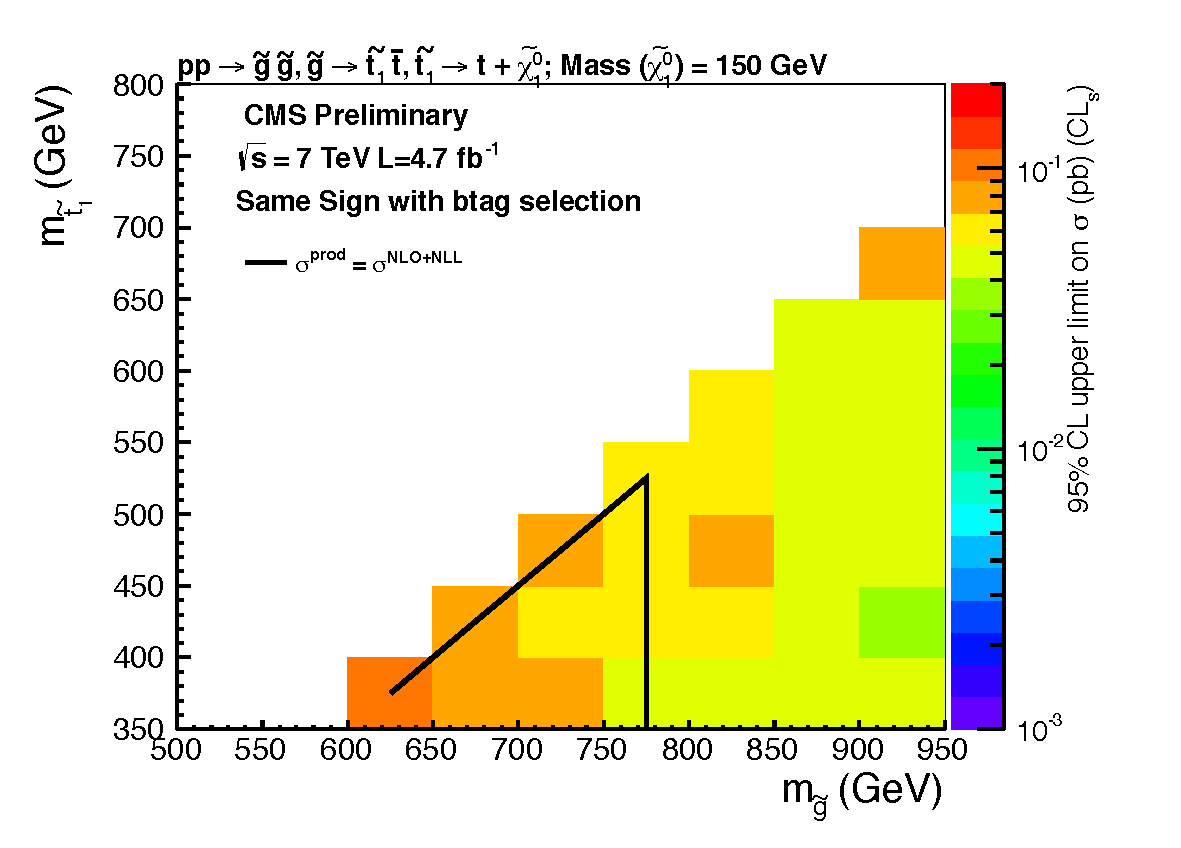
\includegraphics[width=0.47\linewidth]{figs/gluinostop150_zoom.pdf}
\caption{Cross section limits in the $m(\widetilde{g})$ vs. $m(\widetilde{t})$ plane
for $m(\chi_1^0)$ = 50 GeV (left) and 150 GeV (right).  
The bottom plots are versions of the top plots ``zoomed'' into the region
of interest.
\label{fig:mglinoStop}}
\end{center}
\end{figure}


%\subsubsection{What is missing for the $\widetilde{g} \to t\widetilde{t}$ Model}
%\begin{itemize}
%\item Perhaps more details on the MC signal generation???
%\item Need a reference for the {\tt T1tttt} model
%\item Maybe also a plot for LSP mass = 100 GeV? 
%\end{itemize}


\clearpage


\subsection{{\tt T1tttt} Model}
\label{t1ttmodel}

\subsubsection{Theoretical discussion of the {\tt T1tttt} Model}
\label{sec:t1tttheory}
The {\tt T1tttt} simplified model\cite{T1tttt} is very similar to the model of 
Section~\ref{sec:firststopmodel}.  In this model it is assumed that all squarks 
are very heavy, but the stop is somewhat lighter than the other 
quarks\cite{stopVirtual}\cite{stopVirtualPRD}.
Then the gluino would decay as $\widetilde{g} \to t\bar{t}\chi_1^0$ through virtual stops.
Other gluino decay modes would be suppressed because the stop is the lightest squark.
The final state after gluino pair production is $tt\bar{t}\bar{t}\chi_1^0\chi_1^0$,
just as in Section~\ref{sec:firststopmodel}.
The model parameters are $M(\widetilde{g})$ and $M(\chi_1^0)$.



\subsubsection{Signal region definition for the {\tt T1tttt} Model}
\label{sec:t1ttttdefinition}
For each point in parameter space we use the signal region that gives
the best expected limit, see Figure~\ref{fig:t1tttoptimize}.
{\bf (Note: so far the region with 3 btags has not been used).}
The limits include all experimental 
uncertainties.   The JES and btag uncertainties are calculated point-by-point.


\begin{figure}[htb]
\begin{center}
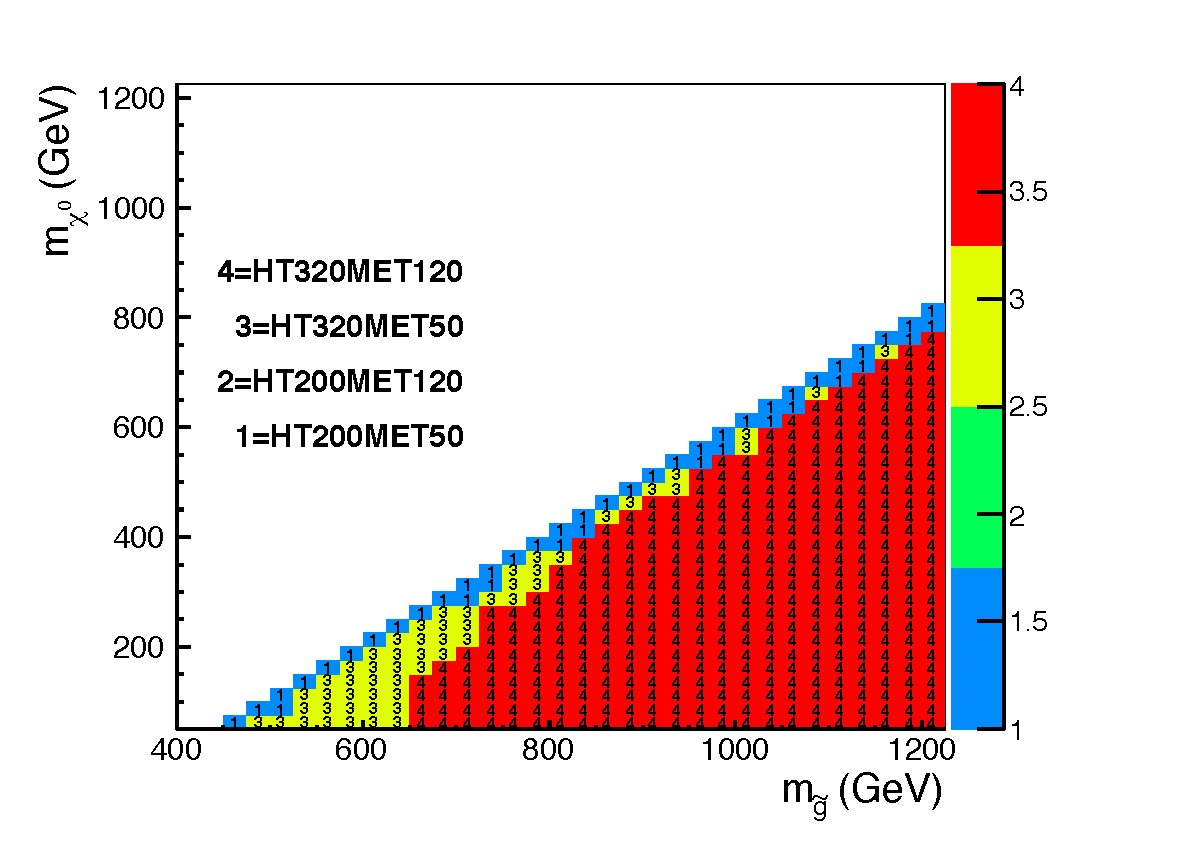
\includegraphics[width=0.4\linewidth]{figs/t1ttttsigreg.pdf}
\caption{The signal region with the best expected limit as a function of 
$m(\widetilde{g})$ vs. $m(\widetilde{t})$ plane for $m(\chi^0_1)$=50 GeV.
The coding is: 1=(200-50), 2=(200-150), 3=(320-50), and 4=(320-120), where
the first (second) number is the $H_T$ (\met) threshold in GeV. The number
of requested btags is 2 or more.
\label{fig:t1tttoptimize}}
\end{center}
\end{figure}


\subsubsection{Limits for the {\tt T1tttt} Model}
\label{sec:t1ttttlimits}
The limit on the production cross-section in this model in the 
gluino mass vs. LSP mass plane shown in Figure~\ref{fig:T1ttttLimit}.  
Using the 
NLO$+$NLL cross-section for gluino pair production, we place a limit
on the mass parameters as shown in Figure~\ref{fig:T1ttttLimit}.
Basically we exclude 
$m(\widetilde{g})$ up to about 800 GeV with a small dependence on 
$m(\chi_1^0)$.

\begin{figure}[htb]
\begin{center}
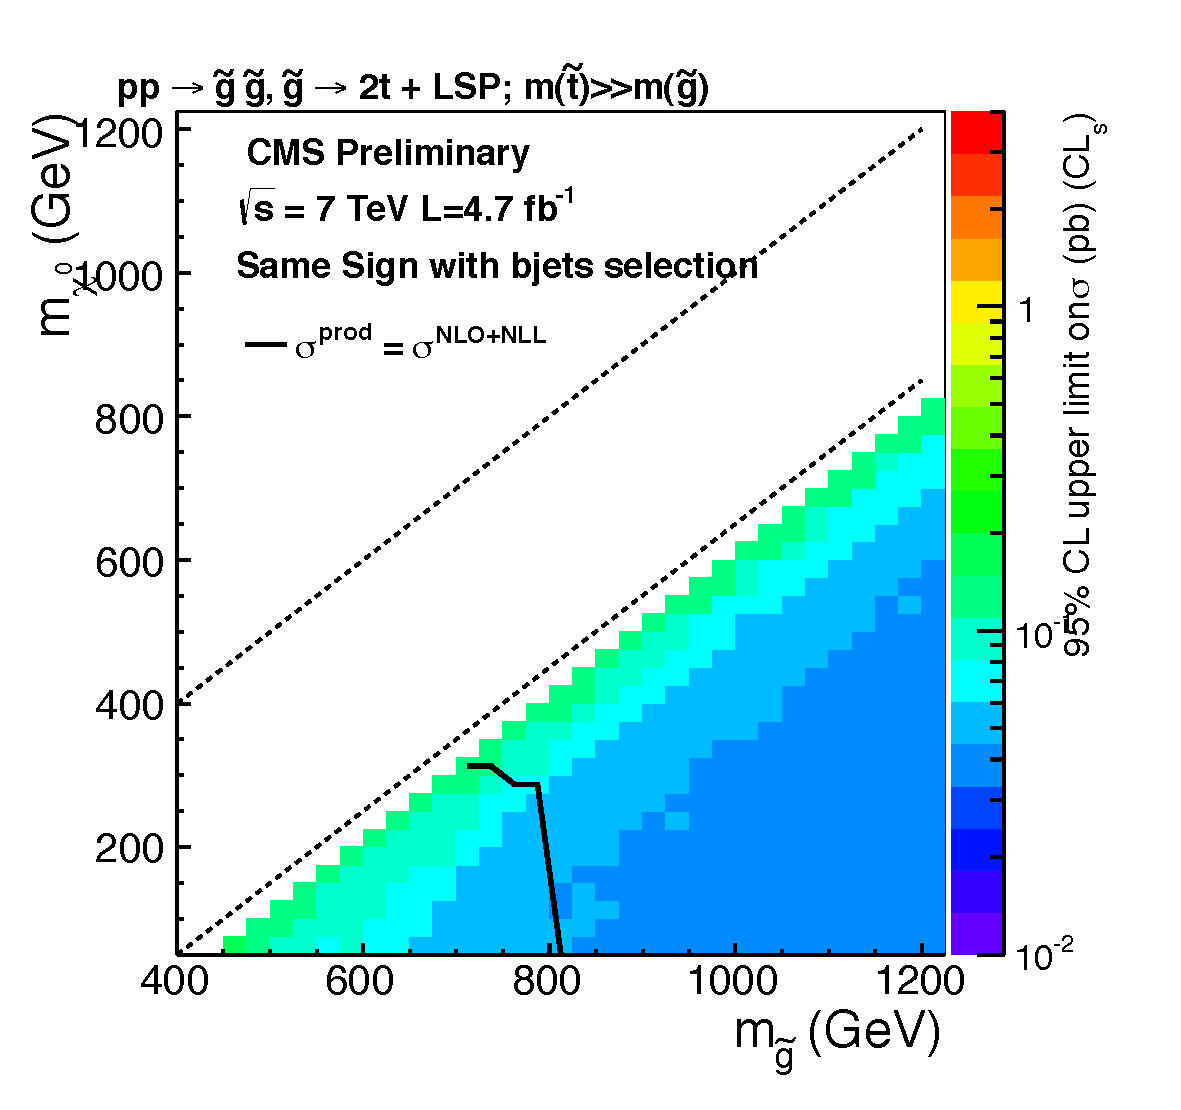
\includegraphics[width=0.48\linewidth]{figs/T1tttt.pdf}
\caption{Cross section limits in the $m(\widetilde{g})$ vs. $m(\chi_1^0)$ plane for the
{\tt T1tttt} model.  
\label{fig:T1ttttLimit}}
\end{center}
\end{figure}

%\subsubsection{What is missing for the {\tt T1tttt} Model}
%\begin{itemize}
%\item Need at least a sentence to say something which signal region contributes.  Or a plot.
%\item Need a reference for the {\tt T1tttt} model
%\end{itemize}


\clearpage

\subsection{Sbottom pair production model}
\label{sec:sbottompair}
In this model we have $pp \to \tilde{b}\tilde{b}$.  The sbottom decays 
as $\tilde{b} \to t\chi^{-}$ followed by $\chi^{-} \to W^- \chi_1^0$. 
The final state is $t\bar{t}W^+W^- \chi_1^0 \chi_1^0$. 
The model parameters are $M(\widetilde{b})$, $M(\chi_1^0)$, and $M(\chi^{\pm})$.
For simplicity we only consider mass parameters such that the $\chi^{-}$ is on shell.

\subsubsection{Signal region definition for the sbottom pair production model}
\label{sec:sbottompairdefinition}
For each point in parameter space we use the signal region that gives
the best expected limit, see Figure~\ref{fig:sbottomoptimize}.
{\bf (Note: so far the region with 3 btags has not been used).}
The limits include all experimental 
uncertainties.   The JES and btag uncertainties are calculated point-by-point.


\begin{figure}[htb]
\begin{center}
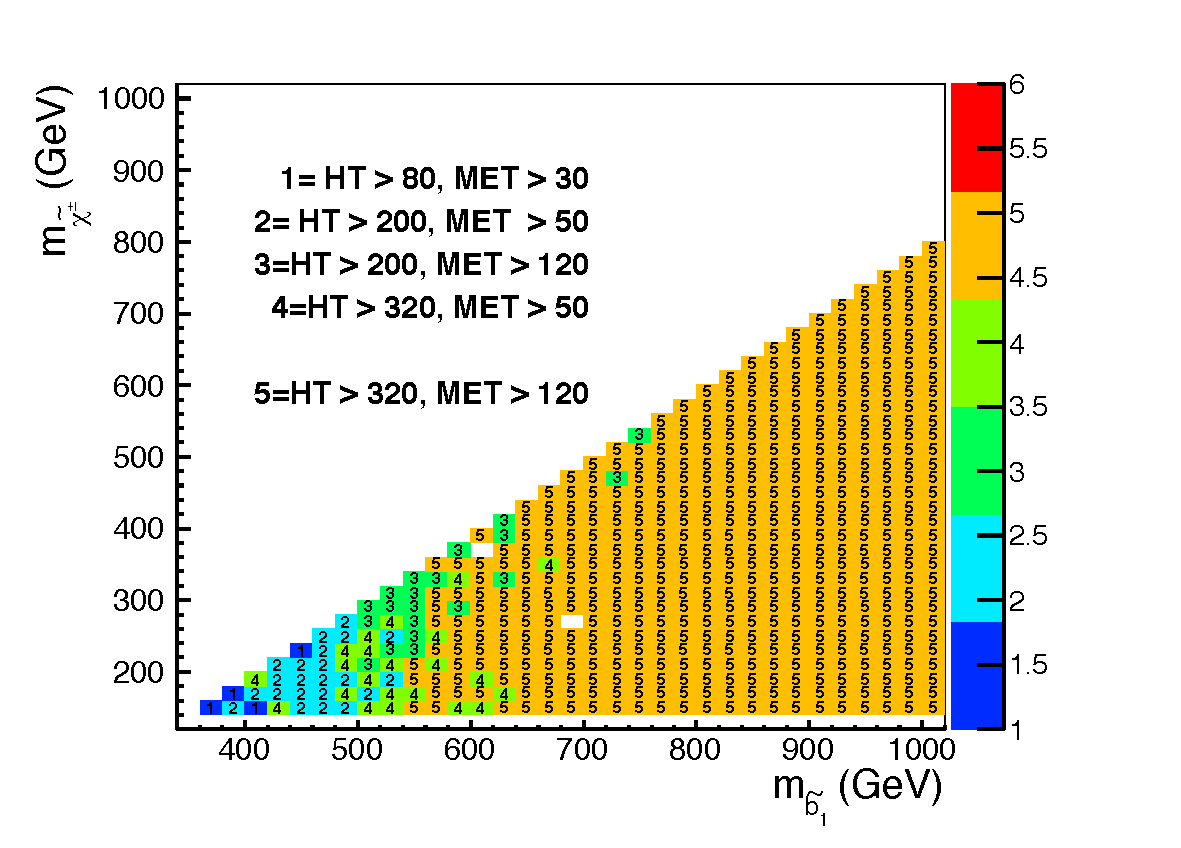
\includegraphics[width=0.5\linewidth]{figs/sbottom_regions.pdf}
\caption{The signal region with the best expected limit as a function of 
$m(\chi^{\pm}))$ vs. $m(\widetilde{b})$ plane for $m(\chi^0_1)$=50 GeV.
The coding is: 1=(80,30),
2=(200-50), 3=(200-150), 4=(320-50), and 5=(320-120), where
the first (second) number is the $H_T$ (\met) threshold in GeV. The number
of requested btags is 2 or more.
\label{fig:sbottomoptimize}}
\end{center}
\end{figure}


\subsubsection{Limits for the sbottom pair production model}
\label{sec:sbottompairlimits}
The limit on the production cross-section in this model in the 
sbottom mass vs. $\chi^{\pm}$ mass plane shown in 
Figure~\ref{fig:sbottomLimit} for 
$m(\chi^0_1)$=50 GeV. 
Using the 
NLO$+$NLL cross-section for gluino pair production, we place a limit
on the mass parameters as shown in Figure~\ref{fig:sbottomLimit}.
We have little sensitivity to the model parameters.
% exclude $m(\widetilde{b})$ up to about 450 GeV for all
% kinematically allowed values of the chargino mass:
% $m(\chi^{\pm})~<~m(\widetilde{b})-m(t)$.

\begin{figure}[htb]
\begin{center}
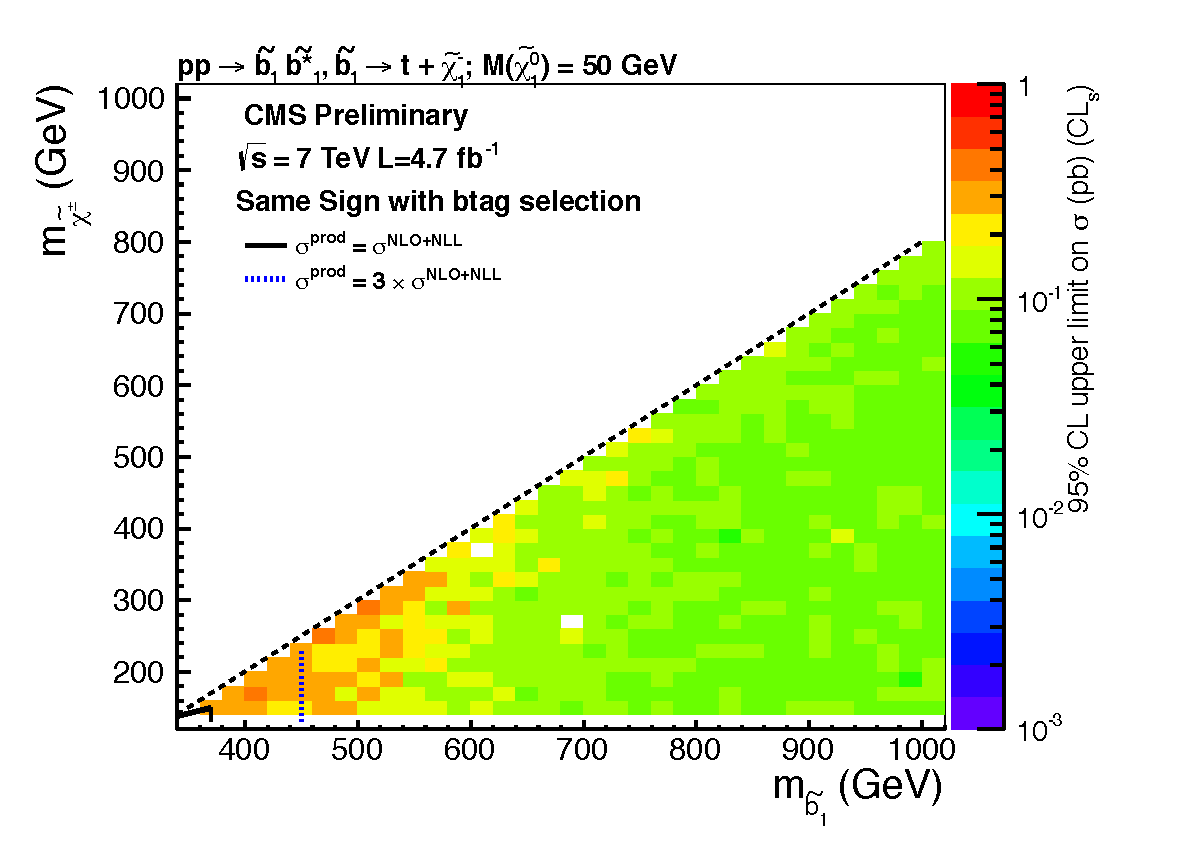
\includegraphics[width=0.48\linewidth]{figs/sbottom_limit.pdf}
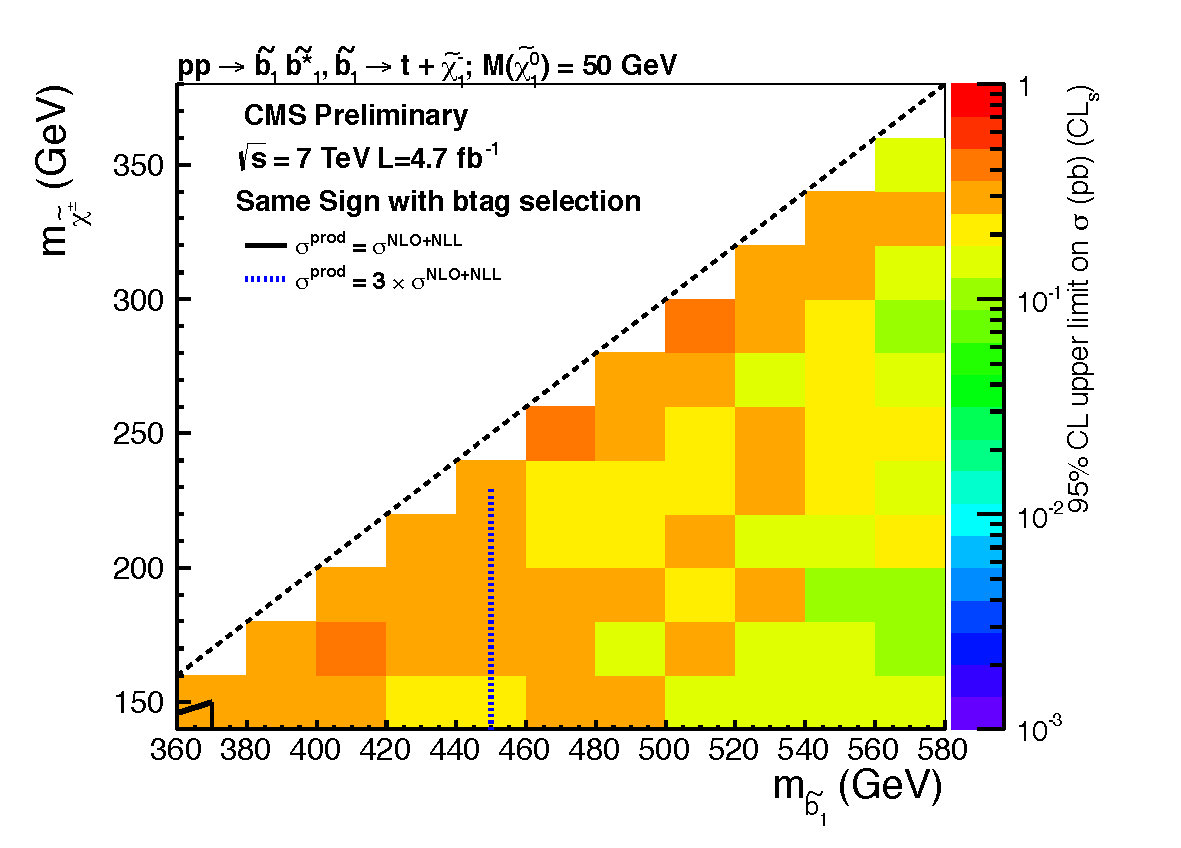
\includegraphics[width=0.48\linewidth]{figs/sbottom_limit_zoom.pdf}
\caption{Cross section limits in the $m(\widetilde{b})$ vs. $m(\chi^{\pm})$ 
plane for the sbottom pair production model with 
$m(\chi^0_1)$=50 GeV.  The rigth plot is a ``zoomed'' in version 
of the left plot.\label{fig:sbottomLimit}}
\end{center}
\end{figure}





%\subsubsection{What is missing for the sbottom pair production model}
%\begin{itemize}
%\item Everything in Sections~\ref{sec:sbottompairdefinition} and \ref{sec:sbottompairlimits}
%\item It would be nice to have a reference.  I am not sure that the references that
%we have on our twiki are appropriate. 
%\item Perhaps more details on the MC signal generation
%\end{itemize}

\clearpage

\subsection{$\widetilde{g} \to \widetilde{b}\bar{b}$ Model}
\label{sec:gbb}
This model is mostly gluino pair production followed by 
$\widetilde{g} \to \widetilde{b}\bar{b}$, $\widetilde{b} \to t \chi^{-}$ and
$\chi^{-} \to W^- \chi_1^0$. 
The final state is $t\bar{t}b\bar{b}W^+W^- \chi_1^0 \chi_1^0$
or $ttb\bar{b}W^+W^- \chi_1^0 \chi_1^0$ $(+ c.c.)$.
The model also includes the $b g \to \widetilde{b} \widetilde{g}$ process,
in which case the final state is
$tb\bar{b}W^+W^- \chi_1^0 \chi_1^0$ $(+ c.c.)$. 
The model parameters are $M(\widetilde{g})$
$M(\widetilde{b})$, $M(\chi_1^0)$, and $M(\chi^{\pm})$.
For simplicity we only consider mass parameters such that the $\chi^{-}$ is on shell.

\subsubsection{Signal region definition for the $\widetilde{g} \to \widetilde{b}\bar{b}$ Model}
\label{sec:gbbdefinition}

\begin{figure}[htb]
\begin{center}
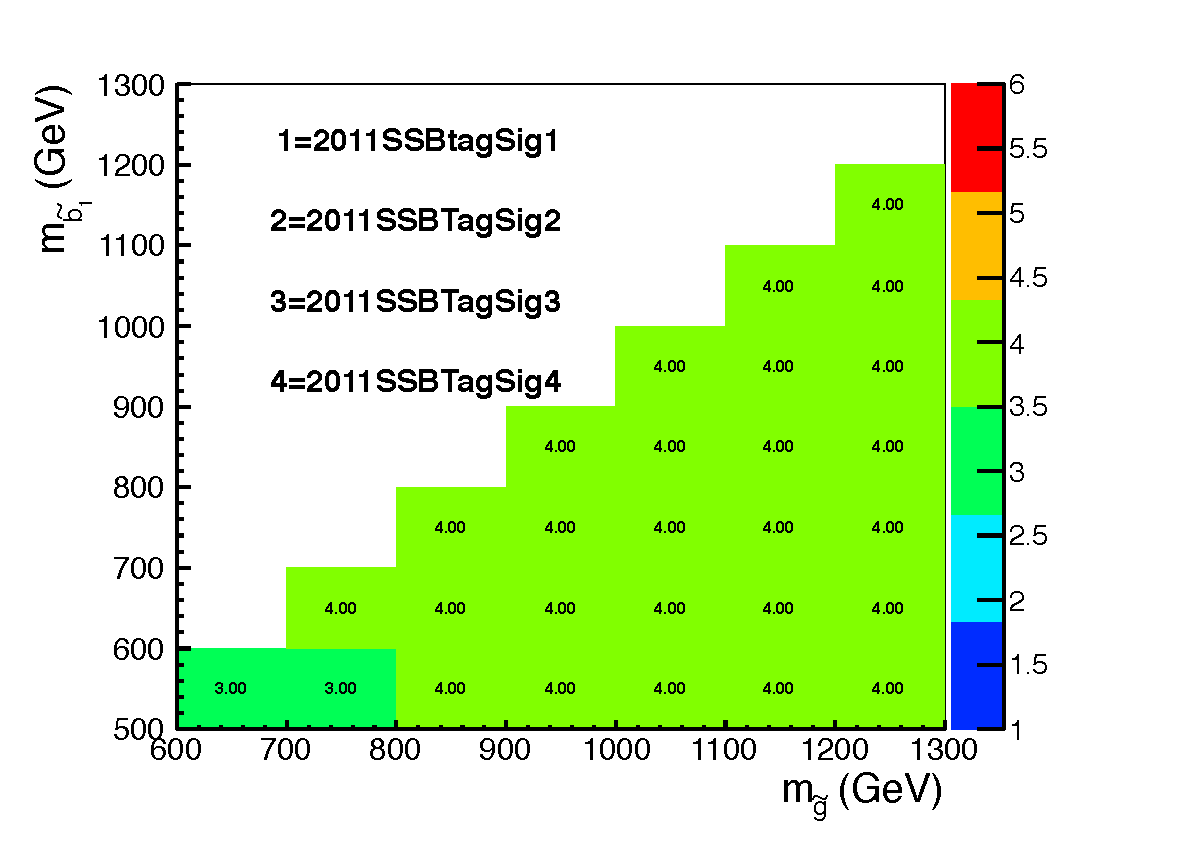
\includegraphics[width=0.65\linewidth]{figs/gl_sb_300_50_regions.pdf}
\caption{The signal region with the best expected limit as a function of 
$m(\widetilde{g}$ vs. $m(\widetilde{b})$ for $m(\chi^0_1)$=50 GeV
and $m(\chi^{\pm})$=200 GeV. 
The coding is: 1=(200-50), 2=(200-150), 3=(320-50), and 4=(320-120), where
the first (second) number is the $H_T$ (\met) threshold in GeV. The number
of requested btags is 2 or more.
\label{fig:gluinosboptimize}}
\end{center}
\end{figure}


For each point in parameter space we use the signal region that gives
the best expected limit.  
{\bf (Note: so far the region with 3 btags has not been used).}
Limits are calculated using all experimental
uncertainties; the JES and btag uncertainties are calculated point-by-point.
An example of this optimization is shown in Figure~\ref{fig:gluinosboptimize},
where we show the choice of signal region that gives the best expected limit
in the $m(\widetilde{g})$ vs. $m(\widetilde{b})$ plane for the choice
$m(\chi^0_1)$=50 GeV and $m(\chi^{\pm})$=200 GeV. 
Roughly speaking we we exclude gluino masses below about 750 GeV for 
all sbottom masses kinematically accessible, {\it i.e.}, 
$m(t)+m(\chi^{\pm})~<~m(\widetilde{b}~<~m(\widetilde{g})$.



\subsubsection{Limits for the $\widetilde{g} \to \widetilde{b}\bar{b}$ Model}
\label{sec:gbblimits}

The limits on the production cross-section in this model in the 
gluino mass vs. sbottom mass plane for two choices of the 
chargino mass and an LSP mass of 50 GeV 
are shown in Figure~\ref{fig:mglinoSbottom}
Using the 
NLO$+$NLL cross-section for gluino pair production, we also place a limit
on the mass parameters of this model.


\begin{figure}[htb]
\begin{center}
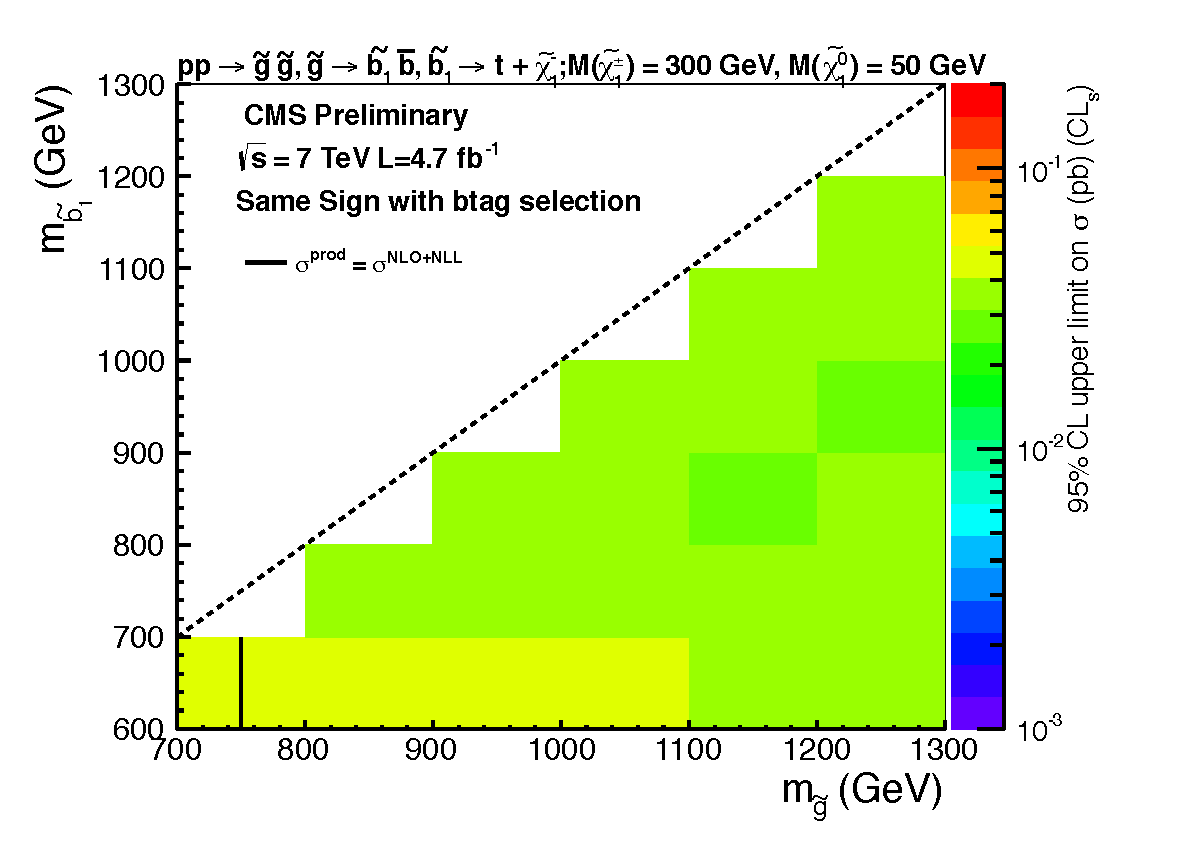
\includegraphics[width=0.47\linewidth]{figs/gl_sb_300_50.pdf}
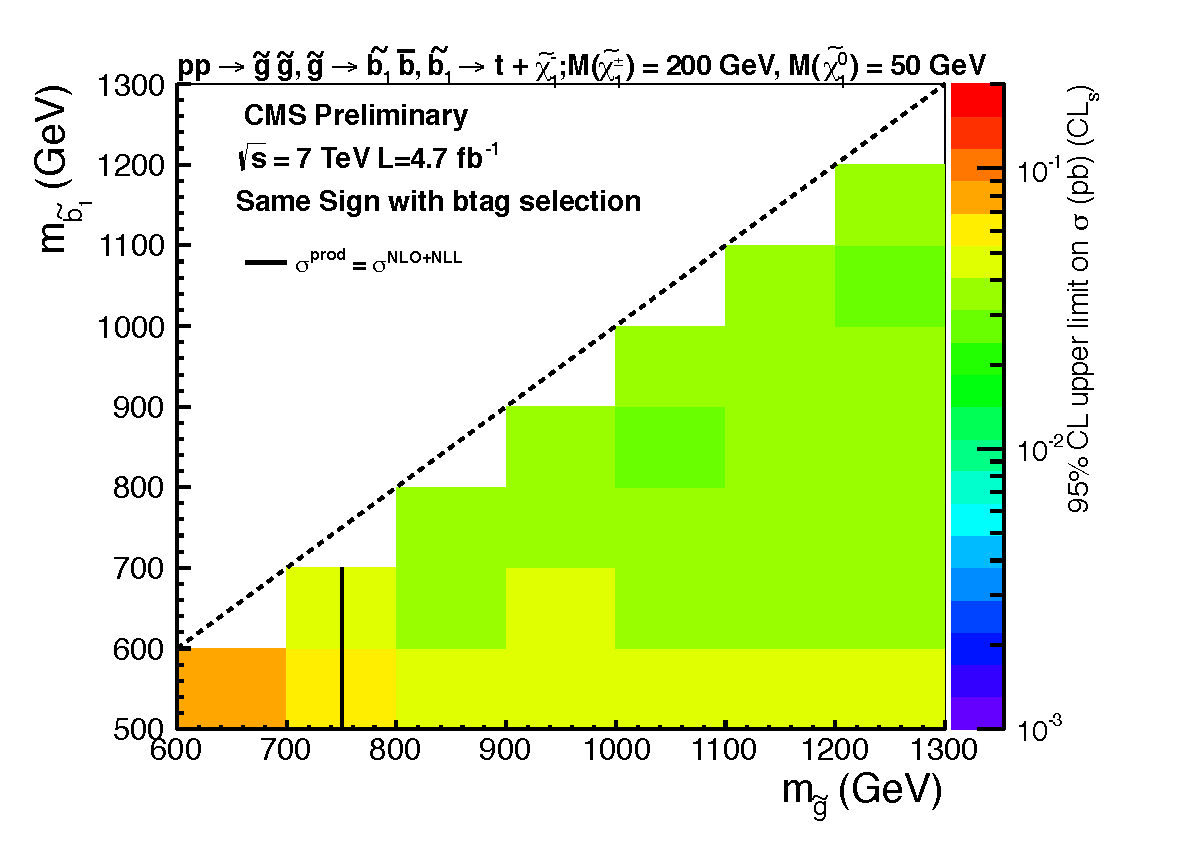
\includegraphics[width=0.47\linewidth]{figs/gl_sb_200_50.pdf}
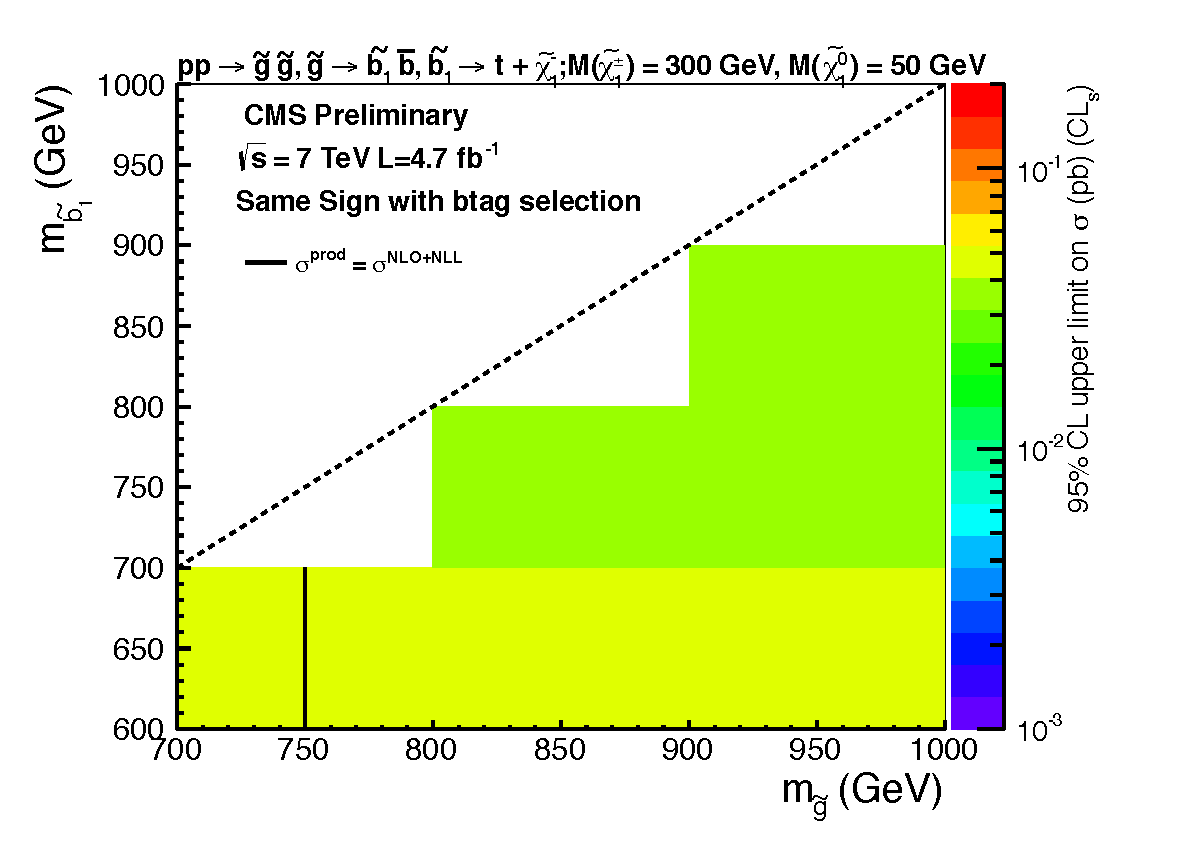
\includegraphics[width=0.47\linewidth]{figs/gl_sb_300_50_zoom.pdf}
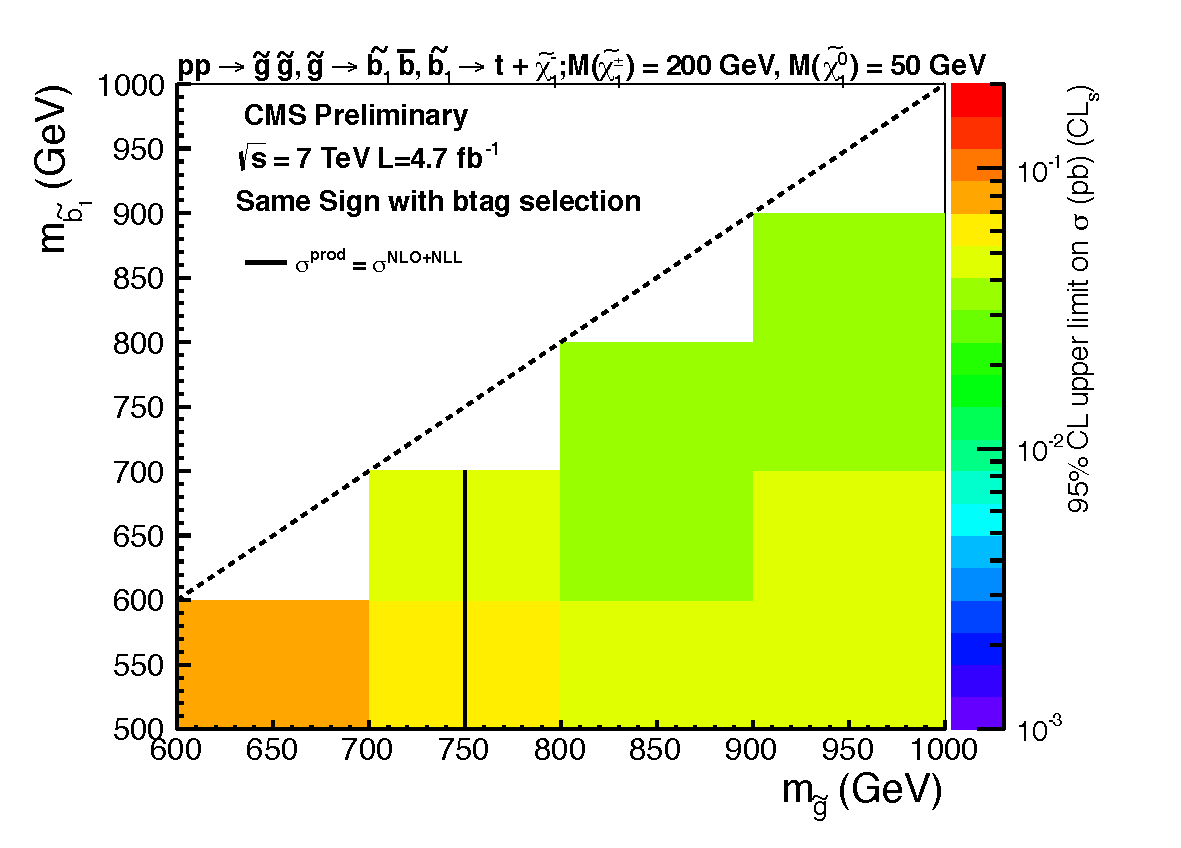
\includegraphics[width=0.47\linewidth]{figs/gl_sb_200_50_zoom.pdf}
\caption{Cross section limits in the $m(\widetilde{g})$ vs. 
$m(\widetilde{b})$ plane
for $m(\chi_1^0)$ = 50 GeV and 
$m(\chi^{\pm})$ = 300 GeV (left) and 200 GeV (right). 
The bottom plots are ``zoomed'' in versions of the top plots.
\label{fig:mglinoSbottom}}
\end{center}
\end{figure}

%\subsubsection{What is missing for the $\widetilde{g} \to \widetilde{b}\bar{b}$ Model}
%\begin{itemize}
%\item Everything in Sections~\ref{sec:gbbdefinition} and \ref{sec:gbblimits}
%\item It would be nice to have a reference.  I am not sure that the 
%references that
%we have on our twiki are appropriate. 
%\item Perhaps more details on the MC signal generation
%\end{itemize}

\clearpage

\section{Conclusion}
\label{sec:conclusion}

We have assessed the sensitivity to mSUGRA of a generic signal characterized by two isolated, high $p_T$ leptons,
significant jet activity, and \met. We performed a scan of the mSUGRA $m_{0}-m_{1/2}$ parameter space and determined  
the expected excluded region in the case of no observed signal as well as the $5\sigma$ sensitivity reach for both SS
and OS dileptons, assuming integrated luminosities of 100 pb$^{-1}$ and 1 fb$^{-1}$. Our results indicate that we are sensitive to a
significant region of the mSUGRA parameter space which extends upon previous results from the Tevatron. 




\clearpage
\begin{thebibliography}{99}

\bibitem{cdf:recentSusy} {CDF Trilepton Search, 2009, CDF/PUB/EXOTIC/PUBLIC/9817};\\
{\small \tt http://www-cdf.fnal.gov/physics/exotic/r2a/20090521.trilepton\_3fb/Welcome.html}
%\bibitem{cdf:recentSusy1} {``Inclusive Search for Squark and Gluino Production in $p\bar{p}$ Collisions at $\sqrt{s}$ = 1.96-TeV'', Phys.Rev.Lett.102:121801, (2009).}
\bibitem{d0:recentSusy} {``Search for associated production of charginos and neutralinos in the trilepton final state using 2.3 fb$^{-1}$ of data'', Phys. Lett. B 680, 34 (2009).}
%\bibitem{d0:recentSusy1} {``Search for squarks and gluinos in events with jets and missing transverse energy using 2.1 fb$^{-1}$ of ppbar collision data at $sqrt(s)=1.96$ TeV'', 
%Phys. Lett. B 660 , 449 (2008).}

\bibitem{osnote} {``Data driven background estimate for a new physics search with opposite sign dileptons''}, CMS AN-2009/130.

\bibitem{ssnote} {``Data driven background study for new physics searches with same sign dileptons at $\sqrt{s} = 10 $ TeV''}, CMS AN-2009/138.

\bibitem{mcsusy}{\tt https://twiki.cern.ch/twiki/bin/viewauth/CMS/SUSYMCRequirements0911}.

\bibitem{fast10}{\tt https://twiki.cern.ch/twiki/bin/view/CMS/SUSY33XScan}.

\bibitem{ww} {``Prospects for measuring the $WW$ production cross section in $pp$ collisions at $\sqrt s = $10 TeV''}, CMS AN-2009/042 and PAS EWK-09-002.

\bibitem{ttbar} {``Expectations for observation of top quark pair production in the dilepton final state with the early CMS data''}, CMS AN-2009/050 and PAS TOP-09-002.

\bibitem{tcmet} {``Correcting Missing Transverse Energy Using Tracks``} CMS AN-2009/022.

\bibitem{conversionnote} {``Study of photon conversion rejection at CMS''}, CMS AN-2009/159.

\bibitem{glbtrk} {\tt https://hypernews.cern.ch/HyperNews/CMS/get/muon/258.html}.

\bibitem{muonid} {``Muon Identification in CMS''}, CMS AN-2008/098.

\bibitem{vplusj} {\tt https://twiki.cern.ch/twiki/bin/view/CMS/VplusJets}.

\bibitem{fakenote} {``Data-driven methods to estimate the electron and muon fake contributions to lepton analyses''}, CMS AN-2009/041.

\bibitem{cite:cousins} {``Evaluation of three methods for calculating statistical significance when incorporating a systematic uncertainty into a test of the background-only hypothesis for a Poisson process''} arXiv:physics/0702156 [physics.data-an]

\bibitem{cite:conway} {``Interval estimation in the presence of nuisance parameters. 1. Bayesian approach''} arXiv:physics/0409129v1 [physics.data-an]

\bibitem{lep:lepsusyreach}{LEP Susy working group: {\tt http://lepsusy.web.cern.ch/lepsusy/} }

\bibitem{bayes}{\tt http://arxiv.org/pdf/physics/0409129}

\bibitem{victor} {\tt http://arxiv.org/pdf/0906.5016}; \\
{\tt http://indico.cern.ch/contributionDisplay.py?contribId=2\&confId=39042}.

\bibitem{summer09}{\tt https://twiki.cern.ch/twiki/bin/view/CMS/SUSY31XProduction}.


\end{thebibliography}


\clearpage
\appendix
\section{Further Fake Rate Discussion}
\label{sec:frFAQ}

Here we address some general questions about the 
Fake Rate (FR) method that have been asked in many 
different occasions.  They are
\begin{enumerate}

\item What about the heavy flavor (HF) composition?  How can you
use the same method in this analysis (where the fakes are mostly
not from HF) and in the untagged analysis (where the fakes are 
mostly from HF)?

\item What is this story of the parton $P_T$ dependence all
about?

\item Why do you take 50\% as an uncertainty?

\item What about signal contamination?

\item If you have an over-prediction in the $t\bar{t}$ 
closure test, why don't you correct for that?

\item Can this be improved?

\end{enumerate}

\subsection{Heavy Flavor composition}
\label{sec:HF}

The first thing to realize is that this question only really 
applies to electrons.  Reasonably high $P_T$
muons in CMS that are not from EWK sources
are dominantly from HF, e.g.,

\begin{itemize}

\item Typically we find that 85-90\% of Fakeable Objects (FO) 
in the QCD MC are from HF. 

\item Even for this analysis, where the HF lepton background
in $t\bar{t}$ has been strongly suppressed by the 
$\geq 2$ btag requirement,
the remaining muon BG is mostly from HF.
This can be best seen by the entries corresponding to the 
lines $t\overline{t}\rightarrow \ell(b\rightarrow \ell)X$
and $t\overline{t}\rightarrow \ell(\slashed{b}\rightarrow \ell)X$
in the $\mu\mu$ column of Table~\ref{tab:yield_baseline}.
This shows that in $t\bar{t}$ MC the predicted BG with 
muons from HF ($\approx$ 0.14 events) is much larger than the 
BG with muons from other sources ($\approx$ 0.02 events).

\end{itemize}

For electrons, the HF dependence can be controlled by
carefully choosing what to use in the ``extrapolation'', {\it i.e.},
what electron requirements are loosened in going from the full
electron selection to the FO selection.  This is discussed in
Reference~\cite{frmethod}.  Briefly, there are three general
ways of defining the FO (V1, V2, V3):

\begin{itemize}
\item    V1 = extrapolate in ID and ISO
\item   V2 = extrapolate in ID only
\item   V3 = extrapolate in ISO only 
\end{itemize}

Extrapolating in ID introduces a HF dependence:
electrons in HF are ``real'', therefore the extrapolation in
ID depends on the HF composition.
If one does not worry about HF, V1 and V2 are sensible
choices, with some distinct advantages over V3, namely:
V2 is the most stable wrt parent parton $P_T$ and
V1 gives the best statistical power.
In the $H \to WW$ analysis, for example, we use V1.
On the other hand, V3 is the most stable against the HF dependence,
but has the worst parton $P_T$ dependence (this dependence
will be discussed in Section~\ref{sec:frpartonpt}).

For SUSY analyses we worry about HF and we use V3, {\it i.e.},
we extrapolate mostly in ISO.
A priori we do not expect a huge dependence of V3 on HF
because the FR of fake electrons from udsg and
HF cannot be that different: in both cases we are 
talking about electrons originating from jets, and the 
properties of jets from udgs are not markedly different 
from those from b.  But this needs to be tested, see below.

We have performed these tests a few times, the best record
of these is Reference~\cite{frmethod}.  Here we summarize 
the results from that note.

We measure the electron FR in data QCD events with an away jet of
40 GeV.  We then apply this FR to FO in QCD events selected 
in the same way but with the away jet b-tagged. We compare
the yield predicted by the FR method 
with the number of electrons passing the cuts in the sample. 
We find a ratio predicted/observed = $1.17 \pm 0.05$.
Note that this test is not 100\% clean.
There is an additional bias because the act
of tagging most likely changes the underlying $P_T$ of the
partons in the event (for example: btagging is not flat vs
jet $P_T$).  

We also perform the same test in MC.  Here we did not have enough stats,
so we had to use the muon-enriched sample. This 
may introduce
yet more bias on the away jet (now the away jet not only
is b-tagged, but it is most likely a $b \to \mu$ decay).
The result on MC is predicted/observed = $0.75 \pm 0.06$.

The bottom line is that we find that enriching the sample in HF changes the 
electron FR by something of order 20\%.  These changes
are due to some combination of HF effects and kinematical
changes in the sample due to the HF enrichment requirements.
We did not try to separate them out.  But the conclusion
is that the method works well enough on both HF-rich and
HF-poor event samples in both data and MC. 

It is also interesting to note that the V1 and V2 FR 
lead to an underprediction in the HF enriched samples,
just as can be argued from first principles.
For data we find  predicted/observed = $0.69 \pm 0.07$
and $0.60 \pm 0.06$ for V1 and V2 respectively; in MC we find 
predicted/observed = $0.27 \pm 0.04$ (V1) and
$0.30 \pm 0.04$ (V2).

Finally, just for fun, we repeat the exercise for muons.
In data we find predicted/observed = $1.03 \pm 0.03$, perfectly
consistent with 1; in MC we find 
this ratio to be $0.81 \pm 0.01$, suggesting that indeed 
there must be some bias in going from the QCD to the muon
enriched sample.

\subsection{Parton $P_T$ dependence}
\label{sec:frpartonpt}

The isolation of a lepton of a given $P_T$ depends 
on the $P_T$ of the mother parton.  This is easy 
to understand, {\em e.g.}, a 19 GeV muon from the
decay of a 20 GeV $b$-quark will be quite isolated
because the rest of the $b$-decay products can only
take up 1 GeV of momentum.  On the other hand a 19 GeV
muon from the decay of a 60 GeV $b$-quark will be much
less isolated.

\begin{figure}[htb]
\begin{center}
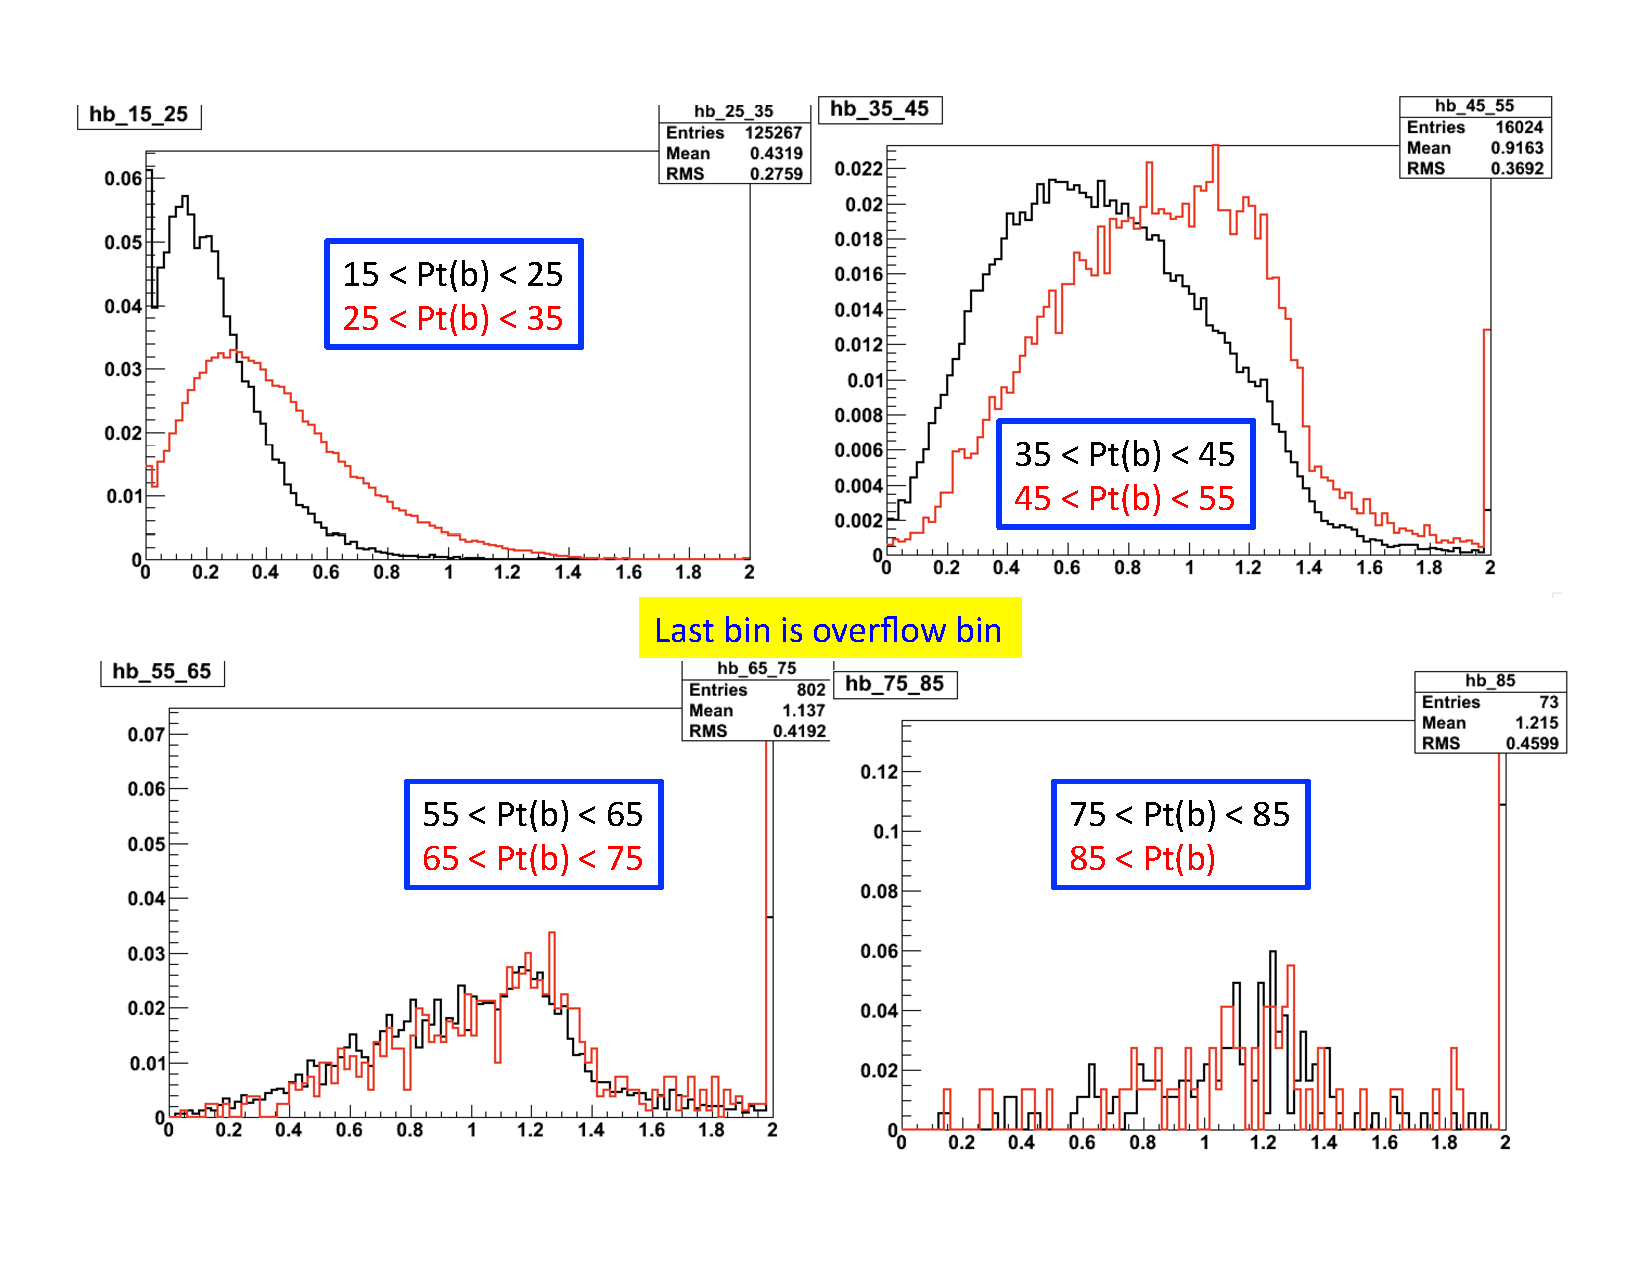
\includegraphics[width=0.75\linewidth]{figs/slavaIso.pdf}
\caption{Isolation for a MC muon from $b \to \mu$ decays
of 14 GeV $< P_T <$ 16 GeV for different intervals of the
parent $b$-quark $P_T$.
\label{fig:slavaIso}}
\end{center}
\end{figure}

This is a \textbf{huge} effect, as can be seen from 
Figure~\ref{fig:slavaIso}.  As a result, extrapolations
in isolation are very sensitive to the parent parton $P_T$
distribution.  We have found that this effect can be mitigated
by reducing the range of isolation over which we extrapolate.
This is why all our isolation extrapolations start from 
iso $<$ 0.4 or 0.6, not iso $< \infty$.

The muon FR is essentially an extrapolation in isolation
since it is almost\footnote{The other handle is 
impact parameter, which is used and 
which is insensitive to the parton $P_T$; however, by itself
it does not provide enough of a lever arm.}
the only handle that can be used
to separate fake muons from EWK muons.
Thus the muon FR, as well as the V3 electron FR, are quite
sensitive to the $P_T$ of the partons from which the 
lepton originates.


Figures~\ref{fig:frmuon} and~\ref{fig:frelectron} show
the muon and electron FR measured in data QCD events with 
different minimum requirements on the away jet $P_T$.  
To the extent that these events are mostly di-jets, 
the away jet $P_T$ is a measure of the $P_T$ of the 
parton from which the lepton originates.  We see that
as we reduce the away jet $P_T$ the FR goes up.
This is what is expected from Figure~\ref{fig:slavaIso}.

We think that it would be a mistake to take the variations
of Figures~\ref{fig:frmuon} and~\ref{fig:frelectron} too 
literally.  The away jet $P_T$ is only an approximation
to the parent parton $P_T$.  Things are not that simple.
For example, there are 3-jet events, there is gluon splitting
inside a jet, and last but not least the $P_T$ distributions
of jets in QCD events is steeply falling, while the $P_T$ 
distribution of jets in the backgrounds to dileptonic SUSY 
sources is not.  

\subsection{Where does the 50\% uncertainty come from?}
\label{sec:FRunc}

Most (all?) systematic uncertainties are judgement calls.
The choice of 50\% (over)covers the variations of 
Figures~\ref{fig:frmuon} and~\ref{fig:frelectron}. It 
(over)covers the variations seen in the HF tests 
(Section~\ref{sec:HF}). It just-about covers the 
closure tests in the $t\bar{t}$ sample (Table~\ref{tab:ttclosure}
in this note, but also results from References~\cite{ssnote2011}
and~\cite{frmethod}).
After playing around with various
options, and after having looked under the hood as we were developing
this methodology as far back as 2008, we have developed a sense
of how much we can trust the method.  It is not perfect:
50\% is perhaps conservative but we feel is a  
realistic estimate.  Finally, 50\% is a nice round number.

\subsection{What about signal contamination?}
\label{sec:sigcont}

The signal can have fake leptons.  These are subtracted
off by the fake rate procedure. To be consistent, in signal 
MC we only count leptons that are truth matched to EWK sources, 
{\em i.e.}, decays of $W$, $Z$, chargino, etc.

The second effect is that in a SUSY event a lepton from EWK
sources can fail the full lepton ID selection but pass the 
looser fakeable object (FO) selection.  These events would then 
increase the count of FO failing the full selection and therefore
increase the background prediction.  To account for this effect
in signal MC, we count the number of such events, we weight
them by their corresonding fake rate factors, and we then 
subtract them off from the acceptance.

Here is a back of the envelope estimate of the size of the effect.
The probability for a lepton to fail the isolation cuts is of the 
order 20\%, see Figure~\ref{fig:lepeffLM6}.  For events with two 
such leptons, the probability that a signal event contaminates
the FO sideband is then $\approx$ 40\%.  These events are then 
weighted by a FR, which is of order 10\%, see 
Figures~\ref{fig:frmuon} and~\ref{fig:frelectron}.  Therefore
the size of the effect that we correct for is of order 4\%.

This last effect can in principle be taken into account ``ab-initio''
in the formulation of the FR method, see for example the discussion
of the parameter $p$ in Reference~\cite{eth}.  However this
causes significant mathematical complications.  To minimize
these complications,  
in applying this method to the generic SS analysis the authors of
Reference~\cite{eth} took a constant FR, independent of $P_T$
and $\eta$.  In addition, there is the question of what exactly
to take for $p$, which is the probability for a signal
lepton to pass the loose cuts but fail the tight cuts.  This
probability is in general a function of the signal itself, {\em
e.g.}, leptons in signals with more hadronic activity will have 
higher probabilities of failing the isolation cut.
To avoid these complications we have decided to leave this 
$p$ factor out, and then apply a correction at the end.



\subsection{Why not correct for the over prediction in $t\bar{t}$ MC?}
\label{sec:frcorrect}

We are not correcting for the overprediction in $t\bar{t}$ MC
(Table~\ref{tab:ttclosure}) for the following reasons.

In a search for new physics we prefer to err on the side of 
overestimating rather than underestimating the background.  The 
resulting ``overoptimism'' of the limits is not a big effect, 
see Table~\ref{tab:outreach}.

We do not fully understand where this overprediction 
comes from, and so we are not comfortable correcting for it.  
The hypothesis is that it is due to differences
in parton $P_T$ between $t\bar{t}$ and the QCD sample where
the FR is measured.  We have evidence that there is
an effect of this sort,
see Section 11.3 and Figure 7 of Reference~\cite{frmethod},
but it was not quantified at the time.  Since then we have 
tried to look at this in more detail. Preliminary results
point in the same direction, but the studies were never completed.

Finally, in the limit that the data and MC QCD FR are the same, the 
correction is equivalent to counting FO in data and 
multiplying them by the ratio of BG leptons to FO in MC.
This seems to us to be going a bit too far away from 
the data driven methodology.  

\subsection{Can the method be improved?}
\label{sec:frimprove}

The method can be improved by reducing the parton $P_T$ dependence
of the FR.  One would need to ``sculpt'' the away-jet $P_T$ 
distribution to better match the expected $P_T$ distribution
of partons in the BG.  This assumes that we can indeed show 
quantitatively that the overprediction in $t\bar{t}$ is from
parton $P_T$.

One of these days, when we are not in a mad rush for ICHEP or Moriond,
or chasing some SUSY scan, or fixing the hyphens in the 
paper drafts, or adding lines of NLL+NLO+PDF uncertainties
to cross-sections of processes that do not exist,
we might actually do it.  However we don't think
that we can go much below something like 30\% on the systematic 
uncertainty, and the improvement will not be a game changer.








\section{Results - Exclusive Yields}
\label{sec:yields_exclusive}


{\bf The information in this appendix is not used 
quantitatively anywhere.}



The tighter \Ht\ and \met\ search regions used for the SUSY production scenarios
and defined in Section~\ref{sec:regions} can be defined exclusively and cover the same
phase space without an overlap between regions:
\begin{enumerate}
     \item Exclusive low-\Ht\ low-\met\ region: $200< \Ht < 320~\GeV, 50 < \met < 120~\GeV$.
     \item Exclusive low-\Ht\ high-\met\ region: $200 < \Ht < 320~\GeV, \met>120~\GeV$.
     \item Exclusive high-\Ht\ low-\met\ region: $\Ht>320~\GeV, 50 < \met < 120~\GeV$.
     \item Exclusive high-\Ht\ high-\met\ region: $\Ht>320~\GeV, \met>120~\GeV$.
\end{enumerate}
The exclusive high-\Ht\ high-\met\ region is the same as its inclusive version.

In the following we report exclusive breakdown of the expected and observed events
in the \Ht-\met\ SUSY search regions.
These are reported in Tables~\ref{tab:yield_excl_ht200met120} to~\ref{tab:yield_excl_ht320met50}.
The formatting of these tables is the same as in Section~\ref{sec:yields}.
Results for the exclusive high-\Ht\ high-\met\ region are not repeated and can be found in Table~\ref{tab:yield_ht320met120}. 




\begin{table}[hbt]
\begin{center}
\begin{tabular}{l | l l l l}
\hline\hline
 Source  &  ee  &  $\mu\mu$  &  e$\mu$  &  all \\
\hline
$t\overline{t}\rightarrow \ell\ell X$ &  0.018 $\pm$  0.014 &  0.000 $\pm$  0.014 &  0.018 $\pm$  0.018 &  0.036 $\pm$  0.023\\
$t\overline{t}$ other &  0.000 $\pm$  0.014 &  0.000 $\pm$  0.014 &  0.000 $\pm$  0.014 &  0.000 $\pm$  0.014\\
$t\overline{t}\rightarrow \ell(b\rightarrow \ell)X$ &  0.000 $\pm$  0.014 &  0.021 $\pm$  0.021 &  0.000 $\pm$  0.014 &  0.021 $\pm$  0.021\\
$t\overline{t}\rightarrow \ell(\slashed{b}\rightarrow \ell)X$ &  0.062 $\pm$  0.032 &  0.000 $\pm$  0.014 &  0.105 $\pm$  0.043 &  0.167 $\pm$  0.054\\
\hline
$t$, s-channel &  0.000 $\pm$  0.061 &  0.000 $\pm$  0.061 &  0.000 $\pm$  0.061 &  0.000 $\pm$  0.061\\
$t$, t-channel &  0.000 $\pm$  0.058 &  0.000 $\pm$  0.058 &  0.000 $\pm$  0.058 &  0.000 $\pm$  0.058\\
$tW$ &  0.000 $\pm$  0.048 &  0.000 $\pm$  0.048 &  0.000 $\pm$  0.048 &  0.000 $\pm$  0.048\\
\hline
$Z\rightarrow ee$ &  0.000 $\pm$  0.457 &  0.000 $\pm$  0.457 &  0.000 $\pm$  0.457 &  0.000 $\pm$  0.457\\
$Z\rightarrow\mu\mu$ &  0.000 $\pm$  0.457 &  0.000 $\pm$  0.457 &  0.000 $\pm$  0.457 &  0.000 $\pm$  0.457\\
$Z\rightarrow\tau\tau$ &  0.000 $\pm$  0.457 &  0.000 $\pm$  0.457 &  0.000 $\pm$  0.457 &  0.000 $\pm$  0.457\\
$W$+jets &  0.000 $\pm$  1.924 &  0.000 $\pm$  1.924 &  0.000 $\pm$  1.924 &  0.000 $\pm$  1.924\\
$WW$ &  0.000 $\pm$  0.020 &  0.000 $\pm$  0.020 &  0.000 $\pm$  0.020 &  0.000 $\pm$  0.020\\
\hline
V$\gamma$ &  0.000 $\pm$  0.264 &  0.000 $\pm$  0.264 &  0.000 $\pm$  0.264 &  0.000 $\pm$  0.264\\
$W\gamma^{*}\rightarrow\ell\nu e e$ &  0.000 $\pm$  0.103 &  0.000 $\pm$  0.103 &  0.000 $\pm$  0.103 &  0.000 $\pm$  0.103\\
$W\gamma^{*}\rightarrow\ell\nu\mu\mu$ &  0.000 $\pm$  0.080 &  0.000 $\pm$  0.080 &  0.000 $\pm$  0.080 &  0.000 $\pm$  0.080\\
$W\gamma^{*}\rightarrow\ell\nu\tau\tau$ &  0.000 $\pm$  0.030 &  0.000 $\pm$  0.030 &  0.000 $\pm$  0.030 &  0.000 $\pm$  0.030\\
$WZ$ &  0.010 $\pm$  0.007 &  0.001 $\pm$  0.003 &   0.000 $\pm$  0.003 &  0.012 $\pm$  0.007\\
$ZZ$ &  0.000 $\pm$   0.000 &  0.000 $\pm$   0.000 &  0.001 $\pm$  0.001 &  0.001 $\pm$  0.001\\
\hline
dp$W^{\pm}W^{\pm}$ &  0.000 $\pm$  0.005 &  0.000 $\pm$  0.005 &  0.000 $\pm$  0.005 &  0.000 $\pm$  0.005\\
sp$W^{-}W^{-}$ &  0.000 $\pm$  0.002 &  0.000 $\pm$  0.002 &  0.001 $\pm$  0.001 &  0.001 $\pm$  0.001\\
sp$W^{+}W^{+}$ &  0.000 $\pm$  0.006 &  0.000 $\pm$  0.006 &  0.000 $\pm$  0.006 &  0.000 $\pm$  0.006\\
$t\overline{t}\gamma$ &  0.000 $\pm$  0.063 &  0.000 $\pm$  0.063 &  0.000 $\pm$  0.063 &  0.000 $\pm$  0.063\\
$t\overline{t}W$ &  0.104 $\pm$  0.011 &  0.129 $\pm$  0.012 &  0.258 $\pm$  0.017 &  0.492 $\pm$  0.024\\
$t\overline{t}Z$ &  0.017 $\pm$  0.004 &  0.025 $\pm$  0.004 &  0.044 $\pm$  0.006 &  0.085 $\pm$  0.008\\
$WW\gamma$ &  0.000 $\pm$  0.016 &  0.000 $\pm$  0.016 &  0.000 $\pm$  0.016 &  0.000 $\pm$  0.016\\
$WWW$ &   0.000 $\pm$   0.000 &   0.000 $\pm$   0.000 &   0.000 $\pm$   0.000 &  0.001 $\pm$   0.000\\
$WWZ$ &  0.000 $\pm$   0.000 &  0.000 $\pm$   0.000 &  0.000 $\pm$   0.000 &  0.000 $\pm$   0.000\\
$WZZ$ &   0.000 $\pm$   0.000 &  0.000 $\pm$   0.000 &   0.000 $\pm$   0.000 &   0.000 $\pm$   0.000\\
$ZZZ$ &  0.000 $\pm$   0.000 &  0.000 $\pm$   0.000 &   0.000 $\pm$   0.000 &   0.000 $\pm$   0.000\\
\hline
Total MC &  0.212 $\pm$  0.038 &  0.176 $\pm$  0.025 &  0.428 $\pm$  0.050 &  0.816 $\pm$  0.067\\
\hline\hline
\hline
LM6 &  0.345 $\pm$  0.046 &  0.403 $\pm$  0.047 &  0.692 $\pm$  0.062 &  1.441 $\pm$  0.090\\
\hline\hline
\hline\hline
 SF  & 0.00 $\pm$ 0.58 & 0.00 $\pm$ 0.37 & 0.32 $\pm$ 0.57 & 0.32 $\pm$ 0.57\\
 DF  & 0.00 $\pm$ 0.14 & 0.00 $\pm$ 0.10 & 0.00 $\pm$ 0.16 & 0.00 $\pm$ 0.16\\
\hline
 SF + DF  & 0.00 $\pm$ 0.50 $\pm$ 0.00 & 0.00 $\pm$ 0.31 $\pm$ 0.00 & 0.32 $\pm$ 0.47 $\pm$ 0.16 & 0.32 $\pm$ 0.47 $\pm$ 0.16\\
\hline\hline
Charge Flips & 0.023 $\pm$ 0.007 $\pm$ 0.005 & - $\pm$ - & 0.022 $\pm$ 0.006 $\pm$ 0.004 & 0.045 $\pm$ 0.009 $\pm$ 0.009\\
\hline\hline
\hline
MC Pred &  0.131 $\pm$  0.014 $\pm$  0.066 &  0.155 $\pm$  0.013 $\pm$  0.078 &  0.306 $\pm$  0.018 $\pm$  0.153 &  0.592 $\pm$  0.026 $\pm$  0.296\\
\hline\hline
Total Pred &  0.154 $\pm$  0.501 $\pm$  0.066 &  0.155 $\pm$  0.315 $\pm$  0.078 &  0.652 $\pm$  0.474 $\pm$  0.223 &  0.962 $\pm$  0.474 $\pm$  0.338\\
\hline\hline
data & 1 & 0 & 1 & 2\\
\hline\hline
\end{tabular}

\end{center}
\caption{\label{tab:yield_excl_ht200met120}Observed event yields in the exclusive low-\Ht\ high-\met\ region
($200< \Ht < $ 320 GeV, \met $>$ 120 GeV)
compared to expectations from simulation alone, and from the data-driven methods.
The upper part of the table is based on simulation only and is used only as a reference.
The lower part is the main result of the analysis.
The SF (DF) contributions are for events with one (two) fake leptons.
The {\em MC Pred} contribution includes contributions from genuine  same-sign lepton
pairs (a sum of the rows from $V\gamma$ down to $ZZZ$).
Entries with zero contributing events are reported with an uncertainty corresponding to one event.
This uncertainty is not added to the total MC contribution.
Systematic uncertainties (the second uncertainty if present)
 are displayed only for the final combined type of background, no systematic
uncertainty is added for estimates with zero entries.
Systematic uncertainties are 100\% correlated among the channels.
}
\end{table}
\clearpage

\begin{table}[hbt]
\begin{center}
\begin{tabular}{l | l l l l}
\hline\hline
 Source  &  ee  &  $\mu\mu$  &  e$\mu$  &  all \\
\hline
$t\overline{t}\rightarrow \ell\ell X$ &  0.151 $\pm$  0.056 &  0.000 $\pm$  0.013 &  0.081 $\pm$  0.036 &  0.232 $\pm$  0.066\\
$t\overline{t}$ other &  0.000 $\pm$  0.013 &  0.000 $\pm$  0.013 &  0.000 $\pm$  0.013 &  0.000 $\pm$  0.013\\
$t\overline{t}\rightarrow \ell(b\rightarrow \ell)X$ &  0.016 $\pm$  0.016 &  0.014 $\pm$  0.014 &  0.025 $\pm$  0.025 &  0.055 $\pm$  0.033\\
$t\overline{t}\rightarrow \ell(\slashed{b}\rightarrow \ell)X$ &  0.135 $\pm$  0.047 &  0.000 $\pm$  0.013 &  0.149 $\pm$  0.054 &  0.284 $\pm$  0.072\\
\hline
$t$, s-channel &  0.000 $\pm$  0.057 &  0.000 $\pm$  0.057 &  0.000 $\pm$  0.057 &  0.000 $\pm$  0.057\\
$t$, t-channel &  0.000 $\pm$  0.055 &  0.000 $\pm$  0.055 &  0.000 $\pm$  0.055 &  0.000 $\pm$  0.055\\
$tW$ &  0.000 $\pm$  0.045 &  0.000 $\pm$  0.045 &  0.016 $\pm$  0.045 &  0.016 $\pm$  0.045\\
\hline
$Z\rightarrow ee$ &  0.000 $\pm$  0.429 &  0.000 $\pm$  0.429 &  0.000 $\pm$  0.429 &  0.000 $\pm$  0.429\\
$Z\rightarrow\mu\mu$ &  0.000 $\pm$  0.429 &  0.000 $\pm$  0.429 &  0.000 $\pm$  0.429 &  0.000 $\pm$  0.429\\
$Z\rightarrow\tau\tau$ &  0.000 $\pm$  0.429 &  0.000 $\pm$  0.429 &  0.000 $\pm$  0.429 &  0.000 $\pm$  0.429\\
$W$+jets &  0.000 $\pm$  1.808 &  0.000 $\pm$  1.808 &  0.000 $\pm$  1.808 &  0.000 $\pm$  1.808\\
$WW$ &  0.000 $\pm$  0.019 &  0.000 $\pm$  0.019 &  0.000 $\pm$  0.019 &  0.000 $\pm$  0.019\\
\hline
V$\gamma$ &  0.000 $\pm$  0.248 &  0.000 $\pm$  0.248 &  0.000 $\pm$  0.248 &  0.000 $\pm$  0.248\\
$W\gamma^{*}\rightarrow\ell\nu e e$ &  0.000 $\pm$  0.097 &  0.000 $\pm$  0.097 &  0.000 $\pm$  0.097 &  0.000 $\pm$  0.097\\
$W\gamma^{*}\rightarrow\ell\nu\mu\mu$ &  0.000 $\pm$  0.075 &  0.000 $\pm$  0.075 &  0.000 $\pm$  0.075 &  0.000 $\pm$  0.075\\
$W\gamma^{*}\rightarrow\ell\nu\tau\tau$ &  0.000 $\pm$  0.028 &  0.000 $\pm$  0.028 &  0.000 $\pm$  0.028 &  0.000 $\pm$  0.028\\
$WZ$ &  0.005 $\pm$  0.005 &  0.012 $\pm$  0.007 &  0.004 $\pm$  0.004 &  0.020 $\pm$  0.009\\
$ZZ$ &  0.000 $\pm$   0.000 &  0.000 $\pm$   0.000 &   0.000 $\pm$   0.000 &   0.000 $\pm$   0.000\\
\hline
dp$W^{\pm}W^{\pm}$ &  0.000 $\pm$  0.004 &  0.000 $\pm$  0.004 &  0.000 $\pm$  0.004 &  0.000 $\pm$  0.004\\
sp$W^{-}W^{-}$ &  0.000 $\pm$  0.001 &  0.000 $\pm$  0.001 &  0.001 $\pm$  0.001 &  0.001 $\pm$  0.001\\
sp$W^{+}W^{+}$ &  0.000 $\pm$  0.006 &  0.000 $\pm$  0.006 &  0.000 $\pm$  0.006 &  0.000 $\pm$  0.006\\
$t\overline{t}\gamma$ &  0.000 $\pm$  0.059 &  0.000 $\pm$  0.059 &  0.000 $\pm$  0.059 &  0.000 $\pm$  0.059\\
$t\overline{t}W$ &  0.147 $\pm$  0.013 &  0.175 $\pm$  0.014 &  0.277 $\pm$  0.017 &  0.599 $\pm$  0.026\\
$t\overline{t}Z$ &  0.027 $\pm$  0.004 &  0.035 $\pm$  0.005 &  0.059 $\pm$  0.006 &  0.120 $\pm$  0.009\\
$WW\gamma$ &  0.000 $\pm$  0.015 &  0.000 $\pm$  0.015 &  0.000 $\pm$  0.015 &  0.000 $\pm$  0.015\\
$WWW$ &  0.000 $\pm$   0.000 &   0.000 $\pm$   0.000 &   0.000 $\pm$   0.000 &   0.000 $\pm$   0.000\\
$WWZ$ &  0.000 $\pm$   0.000 &  0.000 $\pm$   0.000 &  0.001 $\pm$  0.001 &  0.001 $\pm$  0.001\\
$WZZ$ &   0.000 $\pm$   0.000 &   0.000 $\pm$   0.000 &  0.000 $\pm$   0.000 &   0.000 $\pm$   0.000\\
$ZZZ$ &   0.000 $\pm$   0.000 &  0.000 $\pm$   0.000 &   0.000 $\pm$   0.000 &   0.000 $\pm$   0.000\\
\hline
Total MC &  0.480 $\pm$  0.076 &  0.236 $\pm$  0.021 &  0.614 $\pm$  0.074 &  1.329 $\pm$  0.108\\
\hline\hline
\hline
LM6 &  0.000 $\pm$  0.000 &  0.000 $\pm$  0.000 &  0.000 $\pm$  0.000 &  0.000 $\pm$  0.000\\
\hline\hline
\hline\hline
 SF  & 0.24 $\pm$ 0.55 & 0.00 $\pm$ 0.37 & 0.27 $\pm$ 0.59 & 0.51 $\pm$ 0.75\\
 DF  & 0.00 $\pm$ 0.14 & 0.00 $\pm$ 0.10 & 0.00 $\pm$ 0.16 & 0.00 $\pm$ 0.16\\
\hline
 SF + DF  & 0.24 $\pm$ 0.47 $\pm$ 0.12 & 0.00 $\pm$ 0.31 $\pm$ 0.00 & 0.27 $\pm$ 0.49 $\pm$ 0.14 & 0.51 $\pm$ 0.68 $\pm$ 0.25\\
\hline\hline
Charge Flips & 0.065 $\pm$ 0.012 $\pm$ 0.013 & - $\pm$ - & 0.079 $\pm$ 0.011 $\pm$ 0.016 & 0.144 $\pm$ 0.017 $\pm$ 0.029\\
\hline\hline
\hline
MC Pred &  0.178 $\pm$  0.014 $\pm$  0.089 &  0.222 $\pm$  0.016 $\pm$  0.111 &  0.344 $\pm$  0.019 $\pm$  0.172 &  0.744 $\pm$  0.029 $\pm$  0.372\\
\hline\hline
Total Pred &  0.479 $\pm$  0.473 $\pm$  0.148 &  0.222 $\pm$  0.315 $\pm$  0.111 &  0.694 $\pm$  0.495 $\pm$  0.219 &  1.394 $\pm$  0.685 $\pm$  0.451\\
\hline\hline
data & 0 & 0 & 1 & 1\\
\hline\hline
\end{tabular}

\end{center}
\caption{\label{tab:yield_excl_ht200met50}Observed event yields in the exclusive low-\Ht\ low-\met\ region
($200< \Ht < 320$ GeV, $50 < \met < 120$ GeV)
compared to expectations from simulation alone, and from the data-driven methods.
The upper part of the table is based on simulation only and is used only as a reference.
The lower part is the main result of the analysis.
The SF (DF) contributions are for events with one (two) fake leptons.
The {\em MC Pred} contribution includes contributions from genuine  same-sign lepton
pairs (a sum of the rows from $V\gamma$ down to $ZZZ$).
Entries with zero contributing events are reported with an uncertainty corresponding to one event.
This uncertainty is not added to the total MC contribution.
Systematic uncertainties (the second uncertainty if present)
 are displayed only for the final combined type of background, no systematic
uncertainty is added for estimates with zero entries.
Systematic uncertainties are 100\% correlated among the channels.
}
\end{table}
\clearpage

\begin{table}[hbt]
\begin{center}
\begin{tabular}{l | l l l l}
\hline\hline
 Source  &  ee  &  $\mu\mu$  &  e$\mu$  &  all \\
\hline
$t\overline{t}\rightarrow \ell\ell X$ &  0.123 $\pm$  0.042 &  0.000 $\pm$  0.199 &  0.061 $\pm$  0.199 &  0.184 $\pm$  0.055\\
$t\overline{t}$ other &  0.000 $\pm$  0.199 &  0.000 $\pm$  0.199 &  0.000 $\pm$  0.199 &  0.000 $\pm$  0.199\\
$t\overline{t}\rightarrow \ell(b\rightarrow \ell)X$ &  0.051 $\pm$  0.199 &  0.020 $\pm$  0.199 &  0.019 $\pm$  0.199 &  0.090 $\pm$  0.199\\
$t\overline{t}\rightarrow \ell(\slashed{b}\rightarrow \ell)X$ &  0.148 $\pm$  0.051 &  0.016 $\pm$  0.199 &  0.138 $\pm$  0.053 &  0.302 $\pm$  0.075\\
\hline
$t$, s-channel &  0.000 $\pm$  0.057 &  0.000 $\pm$  0.057 &  0.000 $\pm$  0.057 &  0.000 $\pm$  0.057\\
$t$, t-channel &  0.000 $\pm$  0.055 &  0.000 $\pm$  0.055 &  0.000 $\pm$  0.055 &  0.000 $\pm$  0.055\\
$tW$ &  0.000 $\pm$  0.045 &  0.000 $\pm$  0.045 &  0.000 $\pm$  0.045 &  0.000 $\pm$  0.045\\
\hline
$Z\rightarrow ee$ &  0.000 $\pm$  0.429 &  0.000 $\pm$  0.429 &  0.000 $\pm$  0.429 &  0.000 $\pm$  0.429\\
$Z\rightarrow\mu\mu$ &  0.000 $\pm$  0.429 &  0.000 $\pm$  0.429 &  0.000 $\pm$  0.429 &  0.000 $\pm$  0.429\\
$Z\rightarrow\tau\tau$ &  0.000 $\pm$  0.429 &  0.000 $\pm$  0.429 &  0.000 $\pm$  0.429 &  0.000 $\pm$  0.429\\
$W$+jets &  0.000 $\pm$  1.808 &  0.000 $\pm$  1.808 &  0.000 $\pm$  1.808 &  0.000 $\pm$  1.808\\
$WW$ &  0.000 $\pm$  0.019 &  0.000 $\pm$  0.019 &  0.000 $\pm$  0.019 &  0.000 $\pm$  0.019\\
\hline
V$\gamma$ &  0.000 $\pm$  0.248 &  0.000 $\pm$  0.248 &  0.000 $\pm$  0.248 &  0.000 $\pm$  0.248\\
$W\gamma^{*}\rightarrow\ell\nu e e$ &  0.000 $\pm$  0.097 &  0.000 $\pm$  0.097 &  0.000 $\pm$  0.097 &  0.000 $\pm$  0.097\\
$W\gamma^{*}\rightarrow\ell\nu\mu\mu$ &  0.000 $\pm$  0.075 &  0.000 $\pm$  0.075 &  0.000 $\pm$  0.075 &  0.000 $\pm$  0.075\\
$W\gamma^{*}\rightarrow\ell\nu\tau\tau$ &  0.000 $\pm$  0.028 &  0.000 $\pm$  0.028 &  0.000 $\pm$  0.028 &  0.000 $\pm$  0.028\\
$WZ$ &  0.005 $\pm$  0.005 &  0.000 $\pm$  0.003 &  0.006 $\pm$  0.004 &  0.011 $\pm$  0.006\\
$ZZ$ &  0.000 $\pm$   0.000 &  0.000 $\pm$   0.000 &  0.000 $\pm$   0.000 &  0.000 $\pm$   0.000\\
\hline
dp$W^{\pm}W^{\pm}$ &  0.000 $\pm$  0.004 &  0.000 $\pm$  0.004 &  0.000 $\pm$  0.004 &  0.000 $\pm$  0.004\\
sp$W^{-}W^{-}$ &  0.000 $\pm$  0.001 &  0.000 $\pm$  0.001 &  0.000 $\pm$  0.001 &  0.000 $\pm$  0.001\\
sp$W^{+}W^{+}$ &  0.000 $\pm$  0.006 &  0.000 $\pm$  0.006 &  0.000 $\pm$  0.006 &  0.000 $\pm$  0.006\\
$t\overline{t}\gamma$ &  0.000 $\pm$  0.059 &  0.000 $\pm$  0.059 &  0.000 $\pm$  0.059 &  0.000 $\pm$  0.059\\
$t\overline{t}W$ &  0.131 $\pm$  0.012 &  0.134 $\pm$  0.012 &  0.247 $\pm$  0.016 &  0.512 $\pm$  0.024\\
$t\overline{t}Z$ &  0.024 $\pm$  0.004 &  0.041 $\pm$  0.005 &  0.062 $\pm$  0.006 &  0.127 $\pm$  0.009\\
$WW\gamma$ &  0.000 $\pm$  0.015 &  0.000 $\pm$  0.015 &  0.000 $\pm$  0.015 &  0.000 $\pm$  0.015\\
$WWW$ &   0.000 $\pm$   0.000 &   0.000 $\pm$   0.000 &  0.001 $\pm$   0.000 &  0.001 $\pm$  0.001\\
$WWZ$ &  0.000 $\pm$   0.000 &  0.000 $\pm$   0.000 &  0.000 $\pm$   0.000 &  0.000 $\pm$   0.000\\
$WZZ$ &  0.000 $\pm$   0.000 &  0.000 $\pm$   0.000 &  0.000 $\pm$   0.000 &  0.000 $\pm$   0.000\\
$ZZZ$ &  0.000 $\pm$   0.000 &   0.000 $\pm$   0.000 &   0.000 $\pm$   0.000 &   0.000 $\pm$   0.000\\
\hline
Total MC &  0.481 $\pm$  0.076 &  0.211 $\pm$  0.026 &  0.535 $\pm$  0.069 &  1.227 $\pm$  0.106\\
\hline\hline
\hline
LM6 &  0.000 $\pm$  0.000 &  0.000 $\pm$  0.000 &  0.000 $\pm$  0.000 &  0.000 $\pm$  0.000\\
\hline\hline
\hline\hline
 SF  & 0.27 $\pm$ 0.54 & 0.00 $\pm$ 0.37 & 0.39 $\pm$ 0.57 & 0.66 $\pm$ 0.72\\
 DF  & 0.00 $\pm$ 0.14 & 0.00 $\pm$ 0.10 & 0.00 $\pm$ 0.16 & 0.00 $\pm$ 0.16\\
\hline
 SF + DF  & 0.27 $\pm$ 0.45 $\pm$ 0.14 & 0.00 $\pm$ 0.31 $\pm$ 0.00 & 0.39 $\pm$ 0.47 $\pm$ 0.19 & 0.66 $\pm$ 0.65 $\pm$ 0.33\\
\hline\hline
Charge Flips & 0.035 $\pm$ 0.009 $\pm$ 0.007 & - $\pm$ - & 0.057 $\pm$ 0.011 $\pm$ 0.011 & 0.092 $\pm$ 0.014 $\pm$ 0.018\\
\hline\hline
\hline
MC Pred &  0.160 $\pm$  0.014 $\pm$  0.080 &  0.175 $\pm$  0.013 $\pm$  0.088 &  0.316 $\pm$  0.018 $\pm$  0.158 &  0.651 $\pm$  0.026 $\pm$  0.326\\
\hline\hline
Total Pred &  0.468 $\pm$  0.453 $\pm$  0.159 &  0.175 $\pm$  0.315 $\pm$  0.088 &  0.759 $\pm$  0.470 $\pm$  0.250 &  1.402 $\pm$  0.653 $\pm$  0.464\\
\hline\hline
data & 1 & 1 & 0 & 2\\
\hline\hline
\end{tabular}

\end{center}
\caption{\label{tab:yield_excl_ht320met50}Observed event yields in the exclusive high-\Ht\ low-\met\ region
($\Ht > 320$ GeV, $50 < \met < 120 $ GeV)
compared to expectations from simulation alone, and from the data-driven methods.
The upper part of the table is based on simulation only and is used only as a reference.
The lower part is the main result of the analysis.
The SF (DF) contributions are for events with one (two) fake leptons.
The {\em MC Pred} contribution includes contributions from genuine  same-sign lepton
pairs (a sum of the rows from $V\gamma$ down to $ZZZ$).
Entries with zero contributing events are reported with an uncertainty corresponding to one event.
This uncertainty is not added to the total MC contribution.
Systematic uncertainties (the second uncertainty if present)
 are displayed only for the final combined type of background, no systematic
uncertainty is added for estimates with zero entries.
Systematic uncertainties are 100\% correlated among the channels.
}
\end{table}
\clearpage

\section{Results - Additional Breakdown of Yields}
\label{sec:yields_projection}


{\bf The information in this appendix is not used quantitatively anywhere.}

The search regions used in this analysis and defined in Section~\ref{sec:regions} can be defined exclusively in either $\Ht$ or $\met$ as seen in the projection plots in Figure~\ref{fig:htmet}, where the search region breakdown in $\met$ was done as:

\begin{enumerate}
	\item $\Ht > 80~\GeV, 30 < \met < 50~\GeV$.
	\item $\Ht > 80~\GeV, 50 < \met < 120~\GeV$.	
	\item $\Ht > 80~\GeV, \met > 120~\GeV$.
\end{enumerate}	
	
and in $\Ht$ as
	
\begin{enumerate}
	\item $80 < \Ht < 200~\GeV, \met > 30~\GeV$.
	\item $200 < \Ht < 320~\GeV, \met > 30~\GeV$.
	\item $\Ht > 320~\GeV, \met > 30~\GeV$.
\end{enumerate}

In the following we report the breakdown of the expected and observed events
in the \Ht-\met\ SUSY search regions.
These are reported in Tables~\ref{tab:yield_ht80_200met30} to~\ref{tab:yield_ht80met120}.
The formatting of these tables is the same as in Section~\ref{sec:yields}.

\begin{table}[h]
\begin{center}
\begin{tabular}{l | l l l l}
\hline\hline
 Source  &  ee  &  $\mu\mu$  &  e$\mu$  &  all \\
\hline
$t\overline{t}\rightarrow \ell\ell X$ &  0.000 $\pm$  0.014 &  0.000 $\pm$  0.014 &  0.000 $\pm$  0.014 &  0.000 $\pm$  0.014\\
$t\overline{t}$ other &  0.000 $\pm$  0.014 &  0.000 $\pm$  0.014 &  0.000 $\pm$  0.014 &  0.000 $\pm$  0.014\\
$t\overline{t}\rightarrow \ell(b\rightarrow \ell)X$ &  0.000 $\pm$  0.014 &  0.000 $\pm$  0.014 &  0.000 $\pm$  0.014 &  0.000 $\pm$  0.014\\
$t\overline{t}\rightarrow \ell(\slashed{b}\rightarrow \ell)X$ &  0.000 $\pm$  0.014 &  0.000 $\pm$  0.014 &  0.000 $\pm$  0.014 &  0.000 $\pm$  0.014\\
\hline
$t$, s-channel &  0.000 $\pm$  0.061 &  0.000 $\pm$  0.061 &  0.000 $\pm$  0.061 &  0.000 $\pm$  0.061\\
$t$, t-channel &  0.000 $\pm$  0.058 &  0.000 $\pm$  0.058 &  0.000 $\pm$  0.058 &  0.000 $\pm$  0.058\\
$tW$ &  0.000 $\pm$  0.048 &  0.000 $\pm$  0.048 &  0.000 $\pm$  0.048 &  0.000 $\pm$  0.048\\
\hline
$Z\rightarrow ee$ &  0.000 $\pm$  0.457 &  0.000 $\pm$  0.457 &  0.000 $\pm$  0.457 &  0.000 $\pm$  0.457\\
$Z\rightarrow\mu\mu$ &  0.000 $\pm$  0.457 &  0.000 $\pm$  0.457 &  0.000 $\pm$  0.457 &  0.000 $\pm$  0.457\\
$Z\rightarrow\tau\tau$ &  0.000 $\pm$  0.457 &  0.000 $\pm$  0.457 &  0.000 $\pm$  0.457 &  0.000 $\pm$  0.457\\
$W$+jets &  0.000 $\pm$  1.924 &  0.000 $\pm$  1.924 &  0.000 $\pm$  1.924 &  0.000 $\pm$  1.924\\
$WW$ &  0.000 $\pm$  0.020 &  0.000 $\pm$  0.020 &  0.000 $\pm$  0.020 &  0.000 $\pm$  0.020\\
\hline
V$\gamma$ &  0.000 $\pm$  0.264 &  0.000 $\pm$  0.264 &  0.000 $\pm$  0.264 &  0.000 $\pm$  0.264\\
$W\gamma^{*}\rightarrow\ell\nu e e$ &  0.000 $\pm$  0.103 &  0.000 $\pm$  0.103 &  0.000 $\pm$  0.103 &  0.000 $\pm$  0.103\\
$W\gamma^{*}\rightarrow\ell\nu\mu\mu$ &  0.000 $\pm$  0.080 &  0.000 $\pm$  0.080 &  0.000 $\pm$  0.080 &  0.000 $\pm$  0.080\\
$W\gamma^{*}\rightarrow\ell\nu\tau\tau$ &  0.000 $\pm$  0.030 &  0.000 $\pm$  0.030 &  0.000 $\pm$  0.030 &  0.000 $\pm$  0.030\\
$WZ$ &  0.000 $\pm$  0.003 &  0.000 $\pm$  0.003 &  0.000 $\pm$  0.003 &  0.000 $\pm$  0.003\\
$ZZ$ &  0.000 $\pm$   0.000 &  0.000 $\pm$   0.000 &  0.000 $\pm$   0.000 &  0.000 $\pm$   0.000\\
\hline
dp$W^{\pm}W^{\pm}$ &  0.000 $\pm$  0.005 &  0.000 $\pm$  0.005 &  0.000 $\pm$  0.005 &  0.000 $\pm$  0.005\\
sp$W^{-}W^{-}$ &  0.000 $\pm$  0.002 &  0.000 $\pm$  0.002 &  0.000 $\pm$  0.002 &  0.000 $\pm$  0.002\\
sp$W^{+}W^{+}$ &  0.000 $\pm$  0.006 &  0.000 $\pm$  0.006 &  0.000 $\pm$  0.006 &  0.000 $\pm$  0.006\\
$t\overline{t}\gamma$ &  0.000 $\pm$  0.063 &  0.000 $\pm$  0.063 &  0.000 $\pm$  0.063 &  0.000 $\pm$  0.063\\
$t\overline{t}W$ &  0.129 $\pm$  0.012 &  0.214 $\pm$  0.015 &  0.330 $\pm$  0.020 &  0.672 $\pm$  0.028\\
$t\overline{t}Z$ &  0.024 $\pm$  0.004 &  0.037 $\pm$  0.005 &  0.049 $\pm$  0.006 &  0.110 $\pm$  0.009\\
$WW\gamma$ &  0.000 $\pm$  0.016 &  0.000 $\pm$  0.016 &  0.000 $\pm$  0.016 &  0.000 $\pm$  0.016\\
$WWW$ &   0.000 $\pm$   0.000 &   0.000 $\pm$   0.000 &   0.000 $\pm$   0.000 &   0.000 $\pm$   0.000\\
$WWZ$ &   0.000 $\pm$   0.000 &   0.000 $\pm$   0.000 &  0.000 $\pm$   0.000 &   0.000 $\pm$   0.000\\
$WZZ$ &  0.000 $\pm$   0.000 &   0.000 $\pm$   0.000 &  0.001 $\pm$   0.000 &  0.001 $\pm$   0.000\\
$ZZZ$ &   0.000 $\pm$   0.000 &   0.000 $\pm$   0.000 &   0.000 $\pm$   0.000 &   0.000 $\pm$   0.000\\
\hline
Total MC &  0.153 $\pm$  0.013 &  0.252 $\pm$  0.016 &  0.379 $\pm$  0.020 &  0.784 $\pm$  0.029\\
\hline\hline
\hline
LM6 &  0.000 $\pm$  0.000 &  0.000 $\pm$  0.000 &  0.000 $\pm$  0.000 &  0.000 $\pm$  0.000\\
\hline\hline
\hline\hline
 SF  & 0.12 $\pm$ 0.52 & 0.09 $\pm$ 0.13 & 0.57 $\pm$ 0.57 & 0.79 $\pm$ 0.73\\
 DF  & 0.00 $\pm$ 0.14 & 0.02 $\pm$ 0.02 & 0.01 $\pm$ 0.13 & 0.03 $\pm$ 0.13\\
\hline
 SF + DF  & 0.12 $\pm$ 0.43 $\pm$ 0.06 & 0.11 $\pm$ 0.13 $\pm$ 0.06 & 0.58 $\pm$ 0.53 $\pm$ 0.29 & 0.82 $\pm$ 0.69 $\pm$ 0.41\\
\hline\hline
Charge Flips & 0.317 $\pm$ 0.029 $\pm$ 0.063 & - $\pm$ - & 0.325 $\pm$ 0.024 $\pm$ 0.065 & 0.642 $\pm$ 0.037 $\pm$ 0.128\\
\hline\hline
\hline
MC Pred &  0.154 $\pm$  0.013 $\pm$  0.077 &  0.252 $\pm$  0.016 $\pm$  0.126 &  0.380 $\pm$  0.020 $\pm$  0.190 &  0.785 $\pm$  0.029 $\pm$  0.393\\
\hline\hline
Total Pred &  0.593 $\pm$  0.428 $\pm$  0.117 &  0.364 $\pm$  0.131 $\pm$  0.138 &  1.287 $\pm$  0.528 $\pm$  0.354 &  2.244 $\pm$  0.692 $\pm$  0.581\\
\hline\hline
data & 0 & 0 & 1 & 1\\
\hline\hline
\end{tabular}

\end{center}
\caption{\label{tab:yield_ht80_200met30}Observed event yields for 80 $< H_T < $ 200 GeV and \met $>$ 30 GeV
compared to expectations from simulation alone, and from the data-driven methods.
The {\em simulated backgrounds} contribution includes contributions from genuine  same-sign lepton
pairs (WZ, ZZ, leptons from same-sign W from single-parton, double-parton, and $t\bar{t}W$ production, etc.), 
as well as electrons from converted photons in $V\gamma$ production.
Entries with zero contributing events are reported with an uncertainty corresponding to one event.
This uncertainty is not added to the total MC contribution.
Systematic uncertainties (the second uncertainty if present)
 are displayed only for the final combined type of background, no systematic
uncertainty is added for estimates with zero entries.
Systematic uncertainties are 100\% correlated among the channels.
}
\end{table}

\clearpage

\begin{table}[hbt]
\begin{center}
\begin{tabular}{l | l l l l}
\hline\hline
 Source  &  ee  &  $\mu\mu$  &  e$\mu$  &  all \\
\hline
$t\overline{t}\rightarrow \ell\ell X$ &  0.000 $\pm$  0.014 &  0.000 $\pm$  0.014 &  0.000 $\pm$  0.014 &  0.000 $\pm$  0.014\\
$t\overline{t}$ other &  0.000 $\pm$  0.014 &  0.000 $\pm$  0.014 &  0.000 $\pm$  0.014 &  0.000 $\pm$  0.014\\
$t\overline{t}\rightarrow \ell(b\rightarrow \ell)X$ &  0.000 $\pm$  0.014 &  0.000 $\pm$  0.014 &  0.000 $\pm$  0.014 &  0.000 $\pm$  0.014\\
$t\overline{t}\rightarrow \ell(\slashed{b}\rightarrow \ell)X$ &  0.000 $\pm$  0.014 &  0.000 $\pm$  0.014 &  0.000 $\pm$  0.014 &  0.000 $\pm$  0.014\\
\hline
$t$, s-channel &  0.000 $\pm$  0.061 &  0.000 $\pm$  0.061 &  0.000 $\pm$  0.061 &  0.000 $\pm$  0.061\\
$t$, t-channel &  0.082 $\pm$  0.082 &  0.000 $\pm$  0.058 &  0.000 $\pm$  0.058 &  0.082 $\pm$  0.082\\
$tW$ &  0.000 $\pm$  0.048 &  0.000 $\pm$  0.048 &  0.017 $\pm$  0.048 &  0.017 $\pm$  0.048\\
\hline
$Z\rightarrow ee$ &  0.000 $\pm$  0.457 &  0.000 $\pm$  0.457 &  0.000 $\pm$  0.457 &  0.000 $\pm$  0.457\\
$Z\rightarrow\mu\mu$ &  0.000 $\pm$  0.457 &  0.000 $\pm$  0.457 &  0.000 $\pm$  0.457 &  0.000 $\pm$  0.457\\
$Z\rightarrow\tau\tau$ &  0.000 $\pm$  0.457 &  0.000 $\pm$  0.457 &  0.000 $\pm$  0.457 &  0.000 $\pm$  0.457\\
$W$+jets &  0.000 $\pm$  1.924 &  0.000 $\pm$  1.924 &  0.000 $\pm$  1.924 &  0.000 $\pm$  1.924\\
$WW$ &  0.000 $\pm$  0.020 &  0.000 $\pm$  0.020 &  0.000 $\pm$  0.020 &  0.000 $\pm$  0.020\\
\hline
V$\gamma$ &  0.000 $\pm$  0.264 &  0.000 $\pm$  0.264 &  0.000 $\pm$  0.264 &  0.000 $\pm$  0.264\\
$W\gamma^{*}\rightarrow\ell\nu e e$ &  0.000 $\pm$  0.103 &  0.000 $\pm$  0.103 &  0.000 $\pm$  0.103 &  0.000 $\pm$  0.103\\
$W\gamma^{*}\rightarrow\ell\nu\mu\mu$ &  0.000 $\pm$  0.080 &  0.000 $\pm$  0.080 &  0.000 $\pm$  0.080 &  0.000 $\pm$  0.080\\
$W\gamma^{*}\rightarrow\ell\nu\tau\tau$ &  0.000 $\pm$  0.030 &  0.000 $\pm$  0.030 &  0.000 $\pm$  0.030 &  0.000 $\pm$  0.030\\
$WZ$ &  0.000 $\pm$  0.003 &  0.000 $\pm$  0.003 &  0.000 $\pm$  0.003 &  0.000 $\pm$  0.003\\
$ZZ$ &  0.000 $\pm$   0.000 &  0.000 $\pm$   0.000 &  0.000 $\pm$   0.000 &  0.000 $\pm$   0.000\\
\hline
dp$W^{\pm}W^{\pm}$ &  0.000 $\pm$  0.005 &  0.000 $\pm$  0.005 &  0.000 $\pm$  0.005 &  0.000 $\pm$  0.005\\
sp$W^{-}W^{-}$ &  0.000 $\pm$  0.002 &  0.000 $\pm$  0.002 &  0.001 $\pm$  0.001 &  0.001 $\pm$  0.001\\
sp$W^{+}W^{+}$ &  0.000 $\pm$  0.006 &  0.000 $\pm$  0.006 &  0.000 $\pm$  0.006 &  0.000 $\pm$  0.006\\
$t\overline{t}\gamma$ &  0.000 $\pm$  0.063 &  0.000 $\pm$  0.063 &  0.000 $\pm$  0.063 &  0.000 $\pm$  0.063\\
$t\overline{t}W$ &  0.231 $\pm$  0.016 &  0.288 $\pm$  0.018 &  0.498 $\pm$  0.024 &  1.016 $\pm$  0.034\\
$t\overline{t}Z$ &  0.046 $\pm$  0.006 &  0.059 $\pm$  0.007 &  0.106 $\pm$  0.009 &  0.211 $\pm$  0.012\\
$WW\gamma$ &  0.000 $\pm$  0.016 &  0.000 $\pm$  0.016 &  0.000 $\pm$  0.016 &  0.000 $\pm$  0.016\\
$WWW$ &   0.000 $\pm$   0.000 &   0.000 $\pm$   0.000 &   0.000 $\pm$   0.000 &   0.000 $\pm$   0.000\\
$WWZ$ &  0.000 $\pm$   0.000 &  0.000 $\pm$   0.000 &  0.001 $\pm$  0.001 &  0.001 $\pm$  0.001\\
$WZZ$ &   0.000 $\pm$   0.000 &   0.000 $\pm$   0.000 &  0.000 $\pm$   0.000 &   0.000 $\pm$   0.000\\
$ZZZ$ &   0.000 $\pm$   0.000 &   0.000 $\pm$   0.000 &   0.000 $\pm$   0.000 &   0.000 $\pm$   0.000\\
\hline
Total MC &  0.358 $\pm$  0.084 &  0.347 $\pm$  0.019 &  0.624 $\pm$  0.031 &  1.329 $\pm$  0.091\\
\hline\hline
\hline
LM6 &  0.000 $\pm$  0.000 &  0.000 $\pm$  0.000 &  0.000 $\pm$  0.000 &  0.000 $\pm$  0.000\\
\hline\hline
\hline\hline
 SF  & 0.73 $\pm$ 0.63 & 0.10 $\pm$ 0.22 & 0.52 $\pm$ 0.60 & 1.36 $\pm$ 0.87\\
 DF  & 0.04 $\pm$ 0.12 & 0.00 $\pm$ 0.10 & 0.02 $\pm$ 0.13 & 0.05 $\pm$ 0.18\\
\hline
 SF + DF  & 0.77 $\pm$ 0.59 $\pm$ 0.39 & 0.10 $\pm$ 0.10 $\pm$ 0.05 & 0.53 $\pm$ 0.55 $\pm$ 0.27 & 1.41 $\pm$ 0.81 $\pm$ 0.70\\
\hline\hline
Charge Flips & 0.057 $\pm$ 0.008 $\pm$ 0.011 & - $\pm$ - & 0.070 $\pm$ 0.008 $\pm$ 0.014 & 0.127 $\pm$ 0.011 $\pm$ 0.025\\
\hline\hline
\hline
MC Pred &  0.277 $\pm$  0.017 $\pm$  0.138 &  0.348 $\pm$  0.019 $\pm$  0.174 &  0.608 $\pm$  0.026 $\pm$  0.304 &  1.232 $\pm$  0.037 $\pm$  0.616\\
\hline\hline
Total Pred &  1.105 $\pm$  0.588 $\pm$  0.409 &  0.452 $\pm$  0.106 $\pm$  0.182 &  1.212 $\pm$  0.553 $\pm$  0.405 &  2.769 $\pm$  0.814 $\pm$  0.936\\
\hline\hline
data & 1 & 1 & 2 & 4\\
\hline\hline
\end{tabular}

\end{center}
\caption{\label{tab:yield_ht200_320met30}Observed event yields for 200 $< H_T < $ 320 GeV and \met $>$ 30 GeV
compared to expectations from simulation alone, and from the data-driven methods.
The {\em simulated backgrounds} contribution includes contributions from genuine  same-sign lepton
pairs (WZ, ZZ, leptons from same-sign W from single-parton, double-parton, and $t\bar{t}W$ production, etc.), 
as well as electrons from converted photons in $V\gamma$ production.
Entries with zero contributing events are reported with an uncertainty corresponding to one event.
This uncertainty is not added to the total MC contribution.
Systematic uncertainties (the second uncertainty if present)
 are displayed only for the final combined type of background, no systematic
uncertainty is added for estimates with zero entries.
Systematic uncertainties are 100\% correlated among the channels.
}
\end{table}
\clearpage

\begin{table}[hbt]
\begin{center}
\begin{tabular}{l | l l l l}
\hline\hline
 Source  &  ee  &  $\mu\mu$  &  e$\mu$  &  all \\
\hline
$t\overline{t}\rightarrow \ell\ell X$ &  0.000 $\pm$  0.014 &  0.000 $\pm$  0.014 &  0.000 $\pm$  0.014 &  0.000 $\pm$  0.014\\
$t\overline{t}$ other &  0.000 $\pm$  0.014 &  0.000 $\pm$  0.014 &  0.000 $\pm$  0.014 &  0.000 $\pm$  0.014\\
$t\overline{t}\rightarrow \ell(b\rightarrow \ell)X$ &  0.000 $\pm$  0.014 &  0.000 $\pm$  0.014 &  0.000 $\pm$  0.014 &  0.000 $\pm$  0.014\\
$t\overline{t}\rightarrow \ell(\slashed{b}\rightarrow \ell)X$ &  0.000 $\pm$  0.014 &  0.000 $\pm$  0.014 &  0.000 $\pm$  0.014 &  0.000 $\pm$  0.014\\
\hline
$t$, s-channel &  0.000 $\pm$  0.061 &  0.000 $\pm$  0.061 &  0.000 $\pm$  0.061 &  0.000 $\pm$  0.061\\
$t$, t-channel &  0.000 $\pm$  0.058 &  0.000 $\pm$  0.058 &  0.000 $\pm$  0.058 &  0.000 $\pm$  0.058\\
$tW$ &  0.000 $\pm$  0.048 &  0.000 $\pm$  0.048 &  0.000 $\pm$  0.048 &  0.000 $\pm$  0.048\\
\hline
$Z\rightarrow ee$ &  0.000 $\pm$  0.457 &  0.000 $\pm$  0.457 &  0.000 $\pm$  0.457 &  0.000 $\pm$  0.457\\
$Z\rightarrow\mu\mu$ &  0.000 $\pm$  0.457 &  0.000 $\pm$  0.457 &  0.000 $\pm$  0.457 &  0.000 $\pm$  0.457\\
$Z\rightarrow\tau\tau$ &  0.000 $\pm$  0.457 &  0.000 $\pm$  0.457 &  0.000 $\pm$  0.457 &  0.000 $\pm$  0.457\\
$W$+jets &  0.000 $\pm$  1.924 &  0.000 $\pm$  1.924 &  0.000 $\pm$  1.924 &  0.000 $\pm$  1.924\\
$WW$ &  0.000 $\pm$  0.020 &  0.000 $\pm$  0.020 &  0.000 $\pm$  0.020 &  0.000 $\pm$  0.020\\
\hline
V$\gamma$ &  0.000 $\pm$  0.264 &  0.000 $\pm$  0.264 &  0.000 $\pm$  0.264 &  0.000 $\pm$  0.264\\
$W\gamma^{*}\rightarrow\ell\nu e e$ &  0.000 $\pm$  0.103 &  0.000 $\pm$  0.103 &  0.000 $\pm$  0.103 &  0.000 $\pm$  0.103\\
$W\gamma^{*}\rightarrow\ell\nu\mu\mu$ &  0.000 $\pm$  0.080 &  0.000 $\pm$  0.080 &  0.000 $\pm$  0.080 &  0.000 $\pm$  0.080\\
$W\gamma^{*}\rightarrow\ell\nu\tau\tau$ &  0.000 $\pm$  0.030 &  0.000 $\pm$  0.030 &  0.000 $\pm$  0.030 &  0.000 $\pm$  0.030\\
$WZ$ &  0.000 $\pm$  0.003 &  0.000 $\pm$  0.003 &  0.000 $\pm$  0.003 &  0.000 $\pm$  0.003\\
$ZZ$ &  0.000 $\pm$   0.000 &  0.000 $\pm$   0.000 &  0.000 $\pm$   0.000 &  0.000 $\pm$   0.000\\
\hline
dp$W^{\pm}W^{\pm}$ &  0.000 $\pm$  0.005 &  0.000 $\pm$  0.005 &  0.000 $\pm$  0.005 &  0.000 $\pm$  0.005\\
sp$W^{-}W^{-}$ &  0.000 $\pm$  0.002 &  0.000 $\pm$  0.002 &  0.001 $\pm$  0.001 &  0.001 $\pm$  0.001\\
sp$W^{+}W^{+}$ &  0.000 $\pm$  0.006 &  0.000 $\pm$  0.006 &  0.000 $\pm$  0.006 &  0.000 $\pm$  0.006\\
$t\overline{t}\gamma$ &  0.000 $\pm$  0.063 &  0.000 $\pm$  0.063 &  0.000 $\pm$  0.063 &  0.000 $\pm$  0.063\\
$t\overline{t}W$ &  0.247 $\pm$  0.017 &  0.275 $\pm$  0.017 &  0.531 $\pm$  0.025 &  1.053 $\pm$  0.035\\
$t\overline{t}Z$ &  0.057 $\pm$  0.007 &  0.073 $\pm$  0.007 &  0.132 $\pm$  0.010 &  0.262 $\pm$  0.014\\
$WW\gamma$ &  0.000 $\pm$  0.016 &  0.000 $\pm$  0.016 &  0.000 $\pm$  0.016 &  0.000 $\pm$  0.016\\
$WWW$ &   0.000 $\pm$   0.000 &   0.000 $\pm$   0.000 &  0.001 $\pm$  0.001 &  0.002 $\pm$  0.001\\
$WWZ$ &  0.000 $\pm$   0.000 &  0.000 $\pm$   0.000 &  0.000 $\pm$   0.000 &  0.000 $\pm$   0.000\\
$WZZ$ &   0.000 $\pm$   0.000 &   0.000 $\pm$   0.000 &   0.000 $\pm$   0.000 &   0.000 $\pm$   0.000\\
$ZZZ$ &  0.000 $\pm$   0.000 &   0.000 $\pm$   0.000 &   0.000 $\pm$   0.000 &   0.000 $\pm$   0.000\\
\hline
Total MC &  0.305 $\pm$  0.018 &  0.348 $\pm$  0.019 &  0.666 $\pm$  0.027 &  1.319 $\pm$  0.037\\
\hline\hline
\hline
LM6 &  0.000 $\pm$  0.000 &  0.198 $\pm$  0.198 &  0.408 $\pm$  0.293 &  0.606 $\pm$  0.353\\
\hline\hline
\hline\hline
 SF  & 0.27 $\pm$ 0.54 & 0.10 $\pm$ 0.22 & 0.83 $\pm$ 0.63 & 1.21 $\pm$ 0.78\\
 DF  & 0.00 $\pm$ 0.14 & 0.00 $\pm$ 0.10 & 0.00 $\pm$ 0.16 & 0.00 $\pm$ 0.16\\
\hline
 SF + DF  & 0.27 $\pm$ 0.45 $\pm$ 0.14 & 0.10 $\pm$ 0.10 $\pm$ 0.05 & 0.83 $\pm$ 0.54 $\pm$ 0.42 & 1.21 $\pm$ 0.72 $\pm$ 0.60\\
\hline\hline
Charge Flips & 0.069 $\pm$ 0.013 $\pm$ 0.014 & - $\pm$ - & 0.082 $\pm$ 0.013 $\pm$ 0.016 & 0.151 $\pm$ 0.018 $\pm$ 0.030\\
\hline\hline
\hline
MC Pred &  0.305 $\pm$  0.018 $\pm$  0.152 &  0.349 $\pm$  0.019 $\pm$  0.174 &  0.666 $\pm$  0.027 $\pm$  0.333 &  1.319 $\pm$  0.037 $\pm$  0.660\\
\hline\hline
Total Pred &  0.647 $\pm$  0.453 $\pm$  0.205 &  0.453 $\pm$  0.106 $\pm$  0.182 &  1.578 $\pm$  0.545 $\pm$  0.533 &  2.679 $\pm$  0.717 $\pm$  0.895\\
\hline\hline
data & 1 & 1 & 0 & 2\\
\hline\hline
\end{tabular}

\end{center}
\caption{\label{tab:yield_ht320met30t}Observed event yields for $ H_T > $ 320 GeV and \met $>$ 30 GeV
compared to expectations from simulation alone, and from the data-driven methods.
The {\em simulated backgrounds} contribution includes contributions from genuine  same-sign lepton
pairs (WZ, ZZ, leptons from same-sign W from single-parton, double-parton, and $t\bar{t}W$ production, etc.), 
as well as electrons from converted photons in $V\gamma$ production.
Entries with zero contributing events are reported with an uncertainty corresponding to one event.
This uncertainty is not added to the total MC contribution.
Systematic uncertainties (the second uncertainty if present)
 are displayed only for the final combined type of background, no systematic
uncertainty is added for estimates with zero entries.
Systematic uncertainties are 100\% correlated among the channels.
}
\end{table}
\clearpage

\begin{table}[hbt]
\begin{center}
\begin{tabular}{l | l l l l}
\hline\hline
 Source  &  ee  &  $\mu\mu$  &  e$\mu$  &  all \\
\hline
$t\overline{t}\rightarrow \ell\ell X$ &  0.141 $\pm$  0.046 &  0.000 $\pm$  0.199 &  0.201 $\pm$  0.060 &  0.343 $\pm$  0.076\\
$t\overline{t}$ other &  0.000 $\pm$  0.199 &  0.000 $\pm$  0.199 &  0.000 $\pm$  0.199 &  0.000 $\pm$  0.199\\
$t\overline{t}\rightarrow \ell(b\rightarrow \ell)X$ &  0.027 $\pm$  0.199 &  0.066 $\pm$  0.199 &  0.032 $\pm$  0.199 &  0.126 $\pm$  0.045\\
$t\overline{t}\rightarrow \ell(\slashed{b}\rightarrow \ell)X$ &  0.184 $\pm$  0.057 &  0.004 $\pm$  0.199 &  0.166 $\pm$  0.054 &  0.354 $\pm$  0.079\\
\hline
$t$, s-channel &  0.000 $\pm$  0.057 &  0.000 $\pm$  0.057 &  0.000 $\pm$  0.057 &  0.000 $\pm$  0.057\\
$t$, t-channel &  0.077 $\pm$  0.077 &  0.000 $\pm$  0.055 &  0.000 $\pm$  0.055 &  0.077 $\pm$  0.077\\
$tW$ &  0.000 $\pm$  0.045 &  0.000 $\pm$  0.045 &  0.000 $\pm$  0.045 &  0.000 $\pm$  0.045\\
\hline
$Z\rightarrow ee$ &  0.000 $\pm$  0.429 &  0.000 $\pm$  0.429 &  0.000 $\pm$  0.429 &  0.000 $\pm$  0.429\\
$Z\rightarrow\mu\mu$ &  0.000 $\pm$  0.429 &  0.000 $\pm$  0.429 &  0.000 $\pm$  0.429 &  0.000 $\pm$  0.429\\
$Z\rightarrow\tau\tau$ &  0.000 $\pm$  0.429 &  0.000 $\pm$  0.429 &  0.000 $\pm$  0.429 &  0.000 $\pm$  0.429\\
$W$+jets &  0.000 $\pm$  1.808 &  0.000 $\pm$  1.808 &  0.000 $\pm$  1.808 &  0.000 $\pm$  1.808\\
$WW$ &  0.000 $\pm$  0.019 &  0.000 $\pm$  0.019 &  0.000 $\pm$  0.019 &  0.000 $\pm$  0.019\\
\hline
V$\gamma$ &  0.000 $\pm$  0.248 &  0.000 $\pm$  0.248 &  0.000 $\pm$  0.248 &  0.000 $\pm$  0.248\\
$W\gamma^{*}\rightarrow\ell\nu e e$ &  0.000 $\pm$  0.097 &  0.000 $\pm$  0.097 &  0.000 $\pm$  0.097 &  0.000 $\pm$  0.097\\
$W\gamma^{*}\rightarrow\ell\nu\mu\mu$ &  0.000 $\pm$  0.075 &  0.000 $\pm$  0.075 &  0.000 $\pm$  0.075 &  0.000 $\pm$  0.075\\
$W\gamma^{*}\rightarrow\ell\nu\tau\tau$ &  0.000 $\pm$  0.028 &  0.000 $\pm$  0.028 &  0.000 $\pm$  0.028 &  0.000 $\pm$  0.028\\
$WZ$ &  0.003 $\pm$  0.003 &   0.000 $\pm$  0.003 &  0.020 $\pm$  0.010 &  0.023 $\pm$  0.011\\
$ZZ$ &   0.000 $\pm$   0.000 &  0.000 $\pm$   0.000 &   0.000 $\pm$   0.000 &  0.001 $\pm$   0.000\\
\hline
dp$W^{\pm}W^{\pm}$ &  0.000 $\pm$  0.004 &  0.000 $\pm$  0.004 &  0.000 $\pm$  0.004 &  0.000 $\pm$  0.004\\
sp$W^{-}W^{-}$ &  0.000 $\pm$  0.001 &  0.000 $\pm$  0.001 &  0.000 $\pm$  0.001 &  0.000 $\pm$  0.001\\
sp$W^{+}W^{+}$ &  0.000 $\pm$  0.006 &  0.000 $\pm$  0.006 &  0.000 $\pm$  0.006 &  0.000 $\pm$  0.006\\
$t\overline{t}\gamma$ &  0.000 $\pm$  0.059 &  0.000 $\pm$  0.059 &  0.000 $\pm$  0.059 &  0.000 $\pm$  0.059\\
$t\overline{t}W$ &  0.107 $\pm$  0.011 &  0.148 $\pm$  0.012 &  0.274 $\pm$  0.018 &  0.529 $\pm$  0.024\\
$t\overline{t}Z$ &  0.039 $\pm$  0.005 &  0.032 $\pm$  0.004 &  0.081 $\pm$  0.007 &  0.152 $\pm$  0.010\\
$WW\gamma$ &  0.000 $\pm$  0.015 &  0.000 $\pm$  0.015 &  0.000 $\pm$  0.015 &  0.000 $\pm$  0.015\\
$WWW$ &   0.000 $\pm$   0.000 &  0.000 $\pm$   0.000 &   0.000 $\pm$   0.000 &   0.000 $\pm$   0.000\\
$WWZ$ &  0.000 $\pm$   0.000 &  0.000 $\pm$   0.000 &  0.000 $\pm$   0.000 &  0.000 $\pm$   0.000\\
$WZZ$ &   0.000 $\pm$   0.000 &   0.000 $\pm$   0.000 &   0.000 $\pm$   0.000 &  0.001 $\pm$   0.000\\
$ZZZ$ &   0.000 $\pm$   0.000 &   0.000 $\pm$   0.000 &   0.000 $\pm$   0.000 &   0.000 $\pm$   0.000\\
\hline
Total MC &  0.578 $\pm$  0.109 &  0.251 $\pm$  0.037 &  0.776 $\pm$  0.086 &  1.605 $\pm$  0.144\\
\hline\hline
\hline
LM6 &  0.000 $\pm$  0.000 &  0.000 $\pm$  0.000 &  0.000 $\pm$  0.000 &  0.000 $\pm$  0.000\\
\hline\hline
\hline\hline
 SF  & 0.50 $\pm$ 0.65 & 0.30 $\pm$ 0.20 & 0.70 $\pm$ 0.59 & 1.50 $\pm$ 0.90\\
 DF  & 0.04 $\pm$ 0.12 & 0.02 $\pm$ 0.02 & 0.02 $\pm$ 0.13 & 0.07 $\pm$ 0.18\\
\hline
 SF + DF  & 0.53 $\pm$ 0.61 $\pm$ 0.27 & 0.32 $\pm$ 0.20 $\pm$ 0.16 & 0.71 $\pm$ 0.55 $\pm$ 0.36 & 1.57 $\pm$ 0.85 $\pm$ 0.78\\
\hline\hline
Charge Flips & 0.166 $\pm$ 0.020 $\pm$ 0.033 & - $\pm$ - & 0.148 $\pm$ 0.017 $\pm$ 0.030 & 0.313 $\pm$ 0.026 $\pm$ 0.063\\
\hline\hline
\hline
MC Pred &  0.149 $\pm$  0.012 $\pm$  0.075 &  0.181 $\pm$  0.013 $\pm$  0.091 &  0.376 $\pm$  0.022 $\pm$  0.188 &  0.706 $\pm$  0.028 $\pm$  0.353\\
\hline\hline
Total Pred &  0.850 $\pm$  0.611 $\pm$  0.279 &  0.502 $\pm$  0.197 $\pm$  0.184 &  1.238 $\pm$  0.551 $\pm$  0.405 &  2.589 $\pm$  0.846 $\pm$  0.863\\
\hline\hline
data & 0 & 1 & 1 & 2\\
\hline\hline
\end{tabular}

\end{center}
\caption{\label{tab:yield_ht80met30_50}Observed event yields for $ H_T > $ 80 GeV and 30 $<$ \met $<$ 50 GeV
compared to expectations from simulation alone, and from the data-driven methods.
The {\em simulated backgrounds} contribution includes contributions from genuine  same-sign lepton
pairs (WZ, ZZ, leptons from same-sign W from single-parton, double-parton, and $t\bar{t}W$ production, etc.), 
as well as electrons from converted photons in $V\gamma$ production.
Entries with zero contributing events are reported with an uncertainty corresponding to one event.
This uncertainty is not added to the total MC contribution.
Systematic uncertainties (the second uncertainty if present)
 are displayed only for the final combined type of background, no systematic
uncertainty is added for estimates with zero entries.
Systematic uncertainties are 100\% correlated among the channels.
}
\end{table}

\clearpage

\begin{table}[hbt]
\begin{center}
\begin{tabular}{l | l l l l}
\hline\hline
 Source  &  ee  &  $\mu\mu$  &  e$\mu$  &  all \\
\hline
$t\overline{t}\rightarrow \ell\ell X$ &  0.000 $\pm$  0.014 &  0.000 $\pm$  0.014 &  0.000 $\pm$  0.014 &  0.000 $\pm$  0.014\\
$t\overline{t}$ other &  0.000 $\pm$  0.014 &  0.000 $\pm$  0.014 &  0.000 $\pm$  0.014 &  0.000 $\pm$  0.014\\
$t\overline{t}\rightarrow \ell(b\rightarrow \ell)X$ &  0.000 $\pm$  0.014 &  0.000 $\pm$  0.014 &  0.000 $\pm$  0.014 &  0.000 $\pm$  0.014\\
$t\overline{t}\rightarrow \ell(\slashed{b}\rightarrow \ell)X$ &  0.000 $\pm$  0.014 &  0.000 $\pm$  0.014 &  0.000 $\pm$  0.014 &  0.000 $\pm$  0.014\\
\hline
$t$, s-channel &  0.000 $\pm$  0.061 &  0.000 $\pm$  0.061 &  0.000 $\pm$  0.061 &  0.000 $\pm$  0.061\\
$t$, t-channel &  0.000 $\pm$  0.058 &  0.000 $\pm$  0.058 &  0.000 $\pm$  0.058 &  0.000 $\pm$  0.058\\
$tW$ &  0.000 $\pm$  0.048 &  0.000 $\pm$  0.048 &  0.017 $\pm$  0.048 &  0.017 $\pm$  0.048\\
\hline
$Z\rightarrow ee$ &  0.000 $\pm$  0.457 &  0.000 $\pm$  0.457 &  0.000 $\pm$  0.457 &  0.000 $\pm$  0.457\\
$Z\rightarrow\mu\mu$ &  0.000 $\pm$  0.457 &  0.000 $\pm$  0.457 &  0.000 $\pm$  0.457 &  0.000 $\pm$  0.457\\
$Z\rightarrow\tau\tau$ &  0.000 $\pm$  0.457 &  0.000 $\pm$  0.457 &  0.000 $\pm$  0.457 &  0.000 $\pm$  0.457\\
$W$+jets &  0.000 $\pm$  1.924 &  0.000 $\pm$  1.924 &  0.000 $\pm$  1.924 &  0.000 $\pm$  1.924\\
$WW$ &  0.000 $\pm$  0.020 &  0.000 $\pm$  0.020 &  0.000 $\pm$  0.020 &  0.000 $\pm$  0.020\\
\hline
V$\gamma$ &  0.000 $\pm$  0.264 &  0.000 $\pm$  0.264 &  0.000 $\pm$  0.264 &  0.000 $\pm$  0.264\\
$W\gamma^{*}\rightarrow\ell\nu e e$ &  0.000 $\pm$  0.103 &  0.000 $\pm$  0.103 &  0.000 $\pm$  0.103 &  0.000 $\pm$  0.103\\
$W\gamma^{*}\rightarrow\ell\nu\mu\mu$ &  0.000 $\pm$  0.080 &  0.000 $\pm$  0.080 &  0.000 $\pm$  0.080 &  0.000 $\pm$  0.080\\
$W\gamma^{*}\rightarrow\ell\nu\tau\tau$ &  0.000 $\pm$  0.030 &  0.000 $\pm$  0.030 &  0.000 $\pm$  0.030 &  0.000 $\pm$  0.030\\
$WZ$ &  0.000 $\pm$  0.003 &  0.000 $\pm$  0.003 &  0.000 $\pm$  0.003 &  0.000 $\pm$  0.003\\
$ZZ$ &  0.000 $\pm$   0.000 &  0.000 $\pm$   0.000 &  0.000 $\pm$   0.000 &  0.000 $\pm$   0.000\\
\hline
dp$W^{\pm}W^{\pm}$ &  0.000 $\pm$  0.005 &  0.000 $\pm$  0.005 &  0.000 $\pm$  0.005 &  0.000 $\pm$  0.005\\
sp$W^{-}W^{-}$ &  0.000 $\pm$  0.002 &  0.000 $\pm$  0.002 &  0.001 $\pm$  0.001 &  0.001 $\pm$  0.001\\
sp$W^{+}W^{+}$ &  0.000 $\pm$  0.006 &  0.000 $\pm$  0.006 &  0.000 $\pm$  0.006 &  0.000 $\pm$  0.006\\
$t\overline{t}\gamma$ &  0.000 $\pm$  0.063 &  0.000 $\pm$  0.063 &  0.000 $\pm$  0.063 &  0.000 $\pm$  0.063\\
$t\overline{t}W$ &  0.375 $\pm$  0.021 &  0.473 $\pm$  0.023 &  0.778 $\pm$  0.030 &  1.626 $\pm$  0.043\\
$t\overline{t}Z$ &  0.067 $\pm$  0.007 &  0.100 $\pm$  0.009 &  0.157 $\pm$  0.010 &  0.324 $\pm$  0.015\\
$WW\gamma$ &  0.000 $\pm$  0.016 &  0.000 $\pm$  0.016 &  0.000 $\pm$  0.016 &  0.000 $\pm$  0.016\\
$WWW$ &   0.000 $\pm$   0.000 &   0.000 $\pm$   0.000 &  0.001 $\pm$   0.000 &  0.002 $\pm$  0.001\\
$WWZ$ &   0.000 $\pm$   0.000 &   0.000 $\pm$   0.000 &  0.001 $\pm$  0.001 &  0.001 $\pm$  0.001\\
$WZZ$ &   0.000 $\pm$   0.000 &   0.000 $\pm$   0.000 &   0.000 $\pm$   0.000 &  0.001 $\pm$   0.000\\
$ZZZ$ &   0.000 $\pm$   0.000 &   0.000 $\pm$   0.000 &   0.000 $\pm$   0.000 &   0.000 $\pm$   0.000\\
\hline
Total MC &  0.442 $\pm$  0.022 &  0.574 $\pm$  0.025 &  0.956 $\pm$  0.036 &  1.972 $\pm$  0.049\\
\hline\hline
\hline
LM6 &  0.000 $\pm$  0.000 &  0.000 $\pm$  0.000 &  0.000 $\pm$  0.000 &  0.000 $\pm$  0.000\\
\hline\hline
\hline\hline
 SF  & 0.63 $\pm$ 0.60 & 0.00 $\pm$ 0.37 & 0.90 $\pm$ 0.63 & 1.53 $\pm$ 0.82\\
 DF  & 0.00 $\pm$ 0.14 & 0.00 $\pm$ 0.10 & 0.01 $\pm$ 0.13 & 0.01 $\pm$ 0.13\\
\hline
 SF + DF  & 0.63 $\pm$ 0.53 $\pm$ 0.32 & 0.00 $\pm$ 0.31 $\pm$ 0.00 & 0.91 $\pm$ 0.59 $\pm$ 0.45 & 1.54 $\pm$ 0.79 $\pm$ 0.77\\
\hline\hline
Charge Flips & 0.300 $\pm$ 0.028 $\pm$ 0.060 & - $\pm$ - & 0.361 $\pm$ 0.026 $\pm$ 0.072 & 0.661 $\pm$ 0.038 $\pm$ 0.132\\
\hline\hline
\hline
MC Pred &  0.443 $\pm$  0.022 $\pm$  0.221 &  0.575 $\pm$  0.025 $\pm$  0.288 &  0.940 $\pm$  0.032 $\pm$  0.470 &  1.958 $\pm$  0.046 $\pm$  0.979\\
\hline\hline
Total Pred &  1.375 $\pm$  0.527 $\pm$  0.391 &  0.575 $\pm$  0.315 $\pm$  0.288 &  2.209 $\pm$  0.595 $\pm$  0.657 &  4.159 $\pm$  0.795 $\pm$  1.253\\
\hline\hline
data & 1 & 1 & 1 & 3\\
\hline\hline
\end{tabular}

\end{center}
\caption{\label{tab:yield_ht80met50_120}Observed event yields for $ H_T > $ 80 GeV and 50 $<$ \met $<$ 120 GeV
compared to expectations from simulation alone, and from the data-driven methods.
The {\em simulated backgrounds} contribution includes contributions from genuine  same-sign lepton
pairs (WZ, ZZ, leptons from same-sign W from single-parton, double-parton, and $t\bar{t}W$ production, etc.), 
as well as electrons from converted photons in $V\gamma$ production.
Entries with zero contributing events are reported with an uncertainty corresponding to one event.
This uncertainty is not added to the total MC contribution.
Systematic uncertainties (the second uncertainty if present)
 are displayed only for the final combined type of background, no systematic
uncertainty is added for estimates with zero entries.
Systematic uncertainties are 100\% correlated among the channels.
}
\end{table}

\clearpage

\begin{table}[hbt]
\begin{center}
\begin{tabular}{l | l l l l}
\hline\hline
 Source  &  ee  &  $\mu\mu$  &  e$\mu$  &  all \\
\hline
$t\overline{t}\rightarrow \ell\ell X$ &  0.017 $\pm$  0.199 &  0.000 $\pm$  0.199 &  0.017 $\pm$  0.199 &  0.034 $\pm$  0.199\\
$t\overline{t}$ other &  0.000 $\pm$  0.199 &  0.000 $\pm$  0.199 &  0.000 $\pm$  0.199 &  0.000 $\pm$  0.199\\
$t\overline{t}\rightarrow \ell(b\rightarrow \ell)X$ &  0.000 $\pm$  0.199 &  0.020 $\pm$  0.199 &  0.000 $\pm$  0.199 &  0.020 $\pm$  0.199\\
$t\overline{t}\rightarrow \ell(\slashed{b}\rightarrow \ell)X$ &  0.076 $\pm$  0.199 &  0.000 $\pm$  0.199 &  0.139 $\pm$  0.049 &  0.215 $\pm$  0.060\\
\hline
$t$, s-channel &  0.000 $\pm$  0.057 &  0.000 $\pm$  0.057 &  0.000 $\pm$  0.057 &  0.000 $\pm$  0.057\\
$t$, t-channel &  0.000 $\pm$  0.055 &  0.000 $\pm$  0.055 &  0.000 $\pm$  0.055 &  0.000 $\pm$  0.055\\
$tW$ &  0.000 $\pm$  0.045 &  0.000 $\pm$  0.045 &  0.000 $\pm$  0.045 &  0.000 $\pm$  0.045\\
\hline
$Z\rightarrow ee$ &  0.000 $\pm$  0.429 &  0.000 $\pm$  0.429 &  0.000 $\pm$  0.429 &  0.000 $\pm$  0.429\\
$Z\rightarrow\mu\mu$ &  0.000 $\pm$  0.429 &  0.000 $\pm$  0.429 &  0.000 $\pm$  0.429 &  0.000 $\pm$  0.429\\
$Z\rightarrow\tau\tau$ &  0.000 $\pm$  0.429 &  0.000 $\pm$  0.429 &  0.000 $\pm$  0.429 &  0.000 $\pm$  0.429\\
$W$+jets &  0.000 $\pm$  1.808 &  0.000 $\pm$  1.808 &  0.000 $\pm$  1.808 &  0.000 $\pm$  1.808\\
$WW$ &  0.000 $\pm$  0.019 &  0.000 $\pm$  0.019 &  0.000 $\pm$  0.019 &  0.000 $\pm$  0.019\\
\hline
V$\gamma$ &  0.000 $\pm$  0.248 &  0.000 $\pm$  0.248 &  0.000 $\pm$  0.248 &  0.000 $\pm$  0.248\\
$W\gamma^{*}\rightarrow\ell\nu e e$ &  0.000 $\pm$  0.097 &  0.000 $\pm$  0.097 &  0.000 $\pm$  0.097 &  0.000 $\pm$  0.097\\
$W\gamma^{*}\rightarrow\ell\nu\mu\mu$ &  0.000 $\pm$  0.075 &  0.000 $\pm$  0.075 &  0.000 $\pm$  0.075 &  0.000 $\pm$  0.075\\
$W\gamma^{*}\rightarrow\ell\nu\tau\tau$ &  0.000 $\pm$  0.028 &  0.000 $\pm$  0.028 &  0.000 $\pm$  0.028 &  0.000 $\pm$  0.028\\
$WZ$ &  0.010 $\pm$  0.007 &  0.001 $\pm$  0.003 &   0.000 $\pm$  0.003 &  0.011 $\pm$  0.007\\
$ZZ$ &  0.000 $\pm$   0.000 &  0.000 $\pm$   0.000 &  0.001 $\pm$  0.001 &  0.001 $\pm$  0.001\\
\hline
dp$W^{\pm}W^{\pm}$ &  0.000 $\pm$  0.004 &  0.000 $\pm$  0.004 &  0.000 $\pm$  0.004 &  0.000 $\pm$  0.004\\
sp$W^{-}W^{-}$ &  0.000 $\pm$  0.001 &  0.000 $\pm$  0.001 &  0.001 $\pm$  0.001 &  0.001 $\pm$  0.001\\
sp$W^{+}W^{+}$ &  0.000 $\pm$  0.006 &  0.000 $\pm$  0.006 &  0.000 $\pm$  0.006 &  0.000 $\pm$  0.006\\
$t\overline{t}\gamma$ &  0.000 $\pm$  0.059 &  0.000 $\pm$  0.059 &  0.000 $\pm$  0.059 &  0.000 $\pm$  0.059\\
$t\overline{t}W$ &  0.111 $\pm$  0.011 &  0.139 $\pm$  0.012 &  0.273 $\pm$  0.017 &  0.523 $\pm$  0.024\\
$t\overline{t}Z$ &  0.018 $\pm$  0.004 &  0.032 $\pm$  0.005 &  0.042 $\pm$  0.005 &  0.092 $\pm$  0.008\\
$WW\gamma$ &  0.000 $\pm$  0.015 &  0.000 $\pm$  0.015 &  0.000 $\pm$  0.015 &  0.000 $\pm$  0.015\\
$WWW$ &   0.000 $\pm$   0.000 &   0.000 $\pm$   0.000 &   0.000 $\pm$   0.000 &  0.001 $\pm$   0.000\\
$WWZ$ &  0.000 $\pm$   0.000 &  0.000 $\pm$   0.000 &  0.000 $\pm$   0.000 &  0.000 $\pm$   0.000\\
$WZZ$ &   0.000 $\pm$   0.000 &  0.000 $\pm$   0.000 &   0.000 $\pm$   0.000 &   0.000 $\pm$   0.000\\
$ZZZ$ &  0.000 $\pm$   0.000 &  0.000 $\pm$   0.000 &   0.000 $\pm$   0.000 &   0.000 $\pm$   0.000\\
\hline
Total MC &  0.231 $\pm$  0.039 &  0.192 $\pm$  0.024 &  0.475 $\pm$  0.055 &  0.898 $\pm$  0.071\\
\hline\hline
\hline
LM6 &  0.000 $\pm$  0.000 &  0.186 $\pm$  0.186 &  0.383 $\pm$  0.275 &  0.569 $\pm$  0.332\\
\hline\hline
\hline\hline
 SF  & 0.00 $\pm$ 0.58 & 0.00 $\pm$ 0.37 & 0.32 $\pm$ 0.57 & 0.32 $\pm$ 0.57\\
 DF  & 0.00 $\pm$ 0.14 & 0.00 $\pm$ 0.10 & 0.00 $\pm$ 0.16 & 0.00 $\pm$ 0.16\\
\hline
 SF + DF  & 0.00 $\pm$ 0.50 $\pm$ 0.00 & 0.00 $\pm$ 0.31 $\pm$ 0.00 & 0.32 $\pm$ 0.47 $\pm$ 0.16 & 0.32 $\pm$ 0.47 $\pm$ 0.16\\
\hline\hline
Charge Flips & 0.043 $\pm$ 0.010 $\pm$ 0.009 & - $\pm$ - & 0.035 $\pm$ 0.008 $\pm$ 0.007 & 0.078 $\pm$ 0.013 $\pm$ 0.016\\
\hline\hline
\hline
MC Pred &  0.139 $\pm$  0.013 $\pm$  0.069 &  0.172 $\pm$  0.013 $\pm$  0.086 &  0.319 $\pm$  0.018 $\pm$  0.160 &  0.630 $\pm$  0.026 $\pm$  0.315\\
\hline\hline
Total Pred &  0.181 $\pm$  0.501 $\pm$  0.070 &  0.172 $\pm$  0.315 $\pm$  0.086 &  0.679 $\pm$  0.474 $\pm$  0.228 &  1.033 $\pm$  0.474 $\pm$  0.355\\
\hline\hline
data & 1 & 0 & 1 & 2\\
\hline\hline
\end{tabular}

\end{center}
\caption{\label{tab:yield_ht80met120}Observed event yields for $ H_T > $ 80 GeV and \met $>$ 120 GeV
compared to expectations from simulation alone, and from the data-driven methods.
The {\em simulated backgrounds} contribution includes contributions from genuine  same-sign lepton
pairs (WZ, ZZ, leptons from same-sign W from single-parton, double-parton, and $t\bar{t}W$ production, etc.), 
as well as electrons from converted photons in $V\gamma$ production.
Entries with zero contributing events are reported with an uncertainty corresponding to one event.
This uncertainty is not added to the total MC contribution.
Systematic uncertainties (the second uncertainty if present)
 are displayed only for the final combined type of background, no systematic
uncertainty is added for estimates with zero entries.
Systematic uncertainties are 100\% correlated among the channels.
}
\end{table}


\end{document}
